% reducesymm/QFT/blog.tex   compile by  pdflatex blog; bibtex blog
% added Andy Chen and Guopeng Xu                feb 18 2018
% Predrag  switched to github.com               jul  8 2013
% Predrag  switched to pdfLaTeX                 sep  6 2011


\documentclass[10pt,openany]{book}
% says unused [letter] option when
% \documentclass[letter,10pt,openany]{book}


\title{QFT and its discontents
       \\ \Huge a blog}
\author{Predrag Cvitanovi\'{c}}


%%%%%%%%%%%%%%%%%%%%%%%%%%%%%%%%%%%%%%%%%%%%%%%%%%%%%%%%%%%%%%
% GitHub/reducesymm/inputs/setupBlog.tex         main file, internal draft version
% Predrag  switched to pdfLaTeX                 sep  6 2011
% Predrag                                       nov 20 2009

                        %% logical setup, no need to edit %%%%%%%%%%
                        \newif\ifpaper \newif\ifPDF               %%
                        \newif\ifOUP \newif\ifboyscout            %%
                        \newif\ifdasbuch \newif\iftoCB            %%
                        \newif\ifsolutions \newif\ifblog          %%
                        \blogtrue                                 %%
                        \boyscouttrue       %% commented, WWW/drafts %%
                        \dasbuchtrue %% DasBuch, not QFT lectures %%
                        \solutionstrue %% include solutions       %%
                        \paperfalse\PDFtrue %% hyperlinked        %%
                        \OUPfalse \toCBtrue      %% ChaosBook %%%%%%
%%%% Toggle between draft and non-draft versions
%    \boyscoutfalse        % public, for hyperlinked ChaosBook/projects

% \pagestyle{empty}
%\normalsize
%\textwidth 6.0in
%\textheight 8.5in
%\topmargin -0.25in

\usepackage{ifthen}
\usepackage{amsmath,amsfonts,amssymb}
%\usepackage{amsbsy,amsgen,inputs/upmath} % failed: bold greek math
%\usepackage[numbers]{natbib} % Predrag 2010-06-08: to avoid
% Package natbib Error: Bibliography not compatible with author-year citations.
\usepackage{fancyvrb}
\usepackage{url}
\usepackage{alltt}

\usepackage{fancyhdr}
\pagestyle{fancy}
\renewcommand{\sectionmark}[1]%
                {\markright{{\bf\thesection}\ ~~#1}}
%\lhead{\fancyplain{}{\sl\rightmark}}
\rhead[\fancyplain{}{\sl\rightmark}]{}
\cfoot{}
\lfoot{\sl printed \today}
\rfoot{\rm\thepage}

%%% DasBuch compatibility contortions

\usepackage{makeidx}
\usepackage{floatpag}       % apply pagestyles to full page floats.
\usepackage[nooneline]{caption}
\usepackage{../inputs/prlabels}    %% homemade footer package
    \floatpagestyle{empty}  % removes headings for table floats
    \renewcommand{\textfraction}{0.1} % minimum of text on page with float


% \newcounter{chapter}

%%%%%%%%%%%%% PDF VS PS VERSIONS %%%%%%%%%%%%%%%%%%%%
% Predrag  switched to pdfLaTeX                 sep  6 2011

% prepare the public PostScript chapters version:
%  \usepackage[dvips]{graphicx}
%  \usepackage[dvips]{color}     %% dvips allows for colors
%  \usepackage[dvips,colorlinks]{hyperref}

\usepackage[utf8]{inputenc}     % was [latin1]{inputenc}
\usepackage[T1]{fontenc}
\usepackage{times}
\usepackage[pdftex]{graphicx}
\usepackage{array}
\usepackage{verbatim}
\usepackage[pdftex,colorlinks]{hyperref}

\hypersetup{
   pdfauthor=Predrag Cvitanovic,
   pdfkeywords=plane Couette upper branch Newton search Lorenz flow,
   pdftitle=QFT and its discontents - a blog}

%\graphicspath should be replaced by environment variable TEXINPUTS
%\graphicspath{{./Fig/}}     %% directories with graphics files
\graphicspath{{../Fig/}{../figs/}}  %% for each directory
      %% logical chores
        %%%% Toggle between draft and non-draft versions
        %    \boyscoutfalse % public, for hyperlinked ChaosBook/projects
\usepackage[figuresright]{rotating} %% sidewaystables-AJ;
\usepackage{booktabs}
  % % GitHub cvitanov/reducesymm/inputs/biblatex.tex

% Predrag 2015-11-27 activate hyperlinks for journals and URL's

%%%%%%%%%%%%%%%%%%%%%% need elsewhere in the master file %%%%%%%%%%%%%%%%%%%%%%%%%%
   %%%%%%%%%%%%%%%%%%%%%% in the header:
% \usepackage[pdftex,colorlinks]{hyperref}
%   % % GitHub cvitanov/reducesymm/inputs/biblatex.tex

% Predrag 2015-11-27 activate hyperlinks for journals and URL's

%%%%%%%%%%%%%%%%%%%%%% need elsewhere in the master file %%%%%%%%%%%%%%%%%%%%%%%%%%
   %%%%%%%%%%%%%%%%%%%%%% in the header:
% \usepackage[pdftex,colorlinks]{hyperref}
%   % % GitHub cvitanov/reducesymm/inputs/biblatex.tex

% Predrag 2015-11-27 activate hyperlinks for journals and URL's

%%%%%%%%%%%%%%%%%%%%%% need elsewhere in the master file %%%%%%%%%%%%%%%%%%%%%%%%%%
   %%%%%%%%%%%%%%%%%%%%%% in the header:
% \usepackage[pdftex,colorlinks]{hyperref}
% \input{../inputs/biblatex}
% \addbibresource{../bibtex/xxx1.bib}
% \addbibresource{../bibtex/xxx2.bib}
   %%%%%%%%%%%%%%%%%%%%%% in the body, presumably at the very end:
% replace
%   \bibliographystyle{../inputs/adkPCphysrev} % (or whichever .bst style)
%   \bibliography{../bibtex/siminos}
% by
% \printbibliography[
% heading=bibintoc,
% title={References}
% 				  ] %, type=online]  % if not using default "Bibliography"
%%%%%%%%%%%%%%%%%%%%%%%%%%%%%%%%%%%%%%%%%%%%%%%%%%%%%%%%%%%%%


%%%%%%%%%%%%%%%%%%  BIBLATEX MACROS %%%%%%%%%%%%%%%%%%%%%%%%%%%%%%%%
    % AIP, APS style source: https://github.com/josephwright/biblatex-phys
\usepackage[
    backend=bibtex,
    sorting=nyt,
    style=numeric, %alphabetic, % %style=authoryear,
    natbib=true, %false, %
    style=phys, % aps
    biblabel= superscript, % brackets, %
    articletitle=true,  % false, % aps
    chaptertitle=true,  % aip;  % false, % aps
    pageranges = true , % aip: the full range
             % = false, % aps: only the first page being printed
    sortlocale=en_US,
    firstinits=true,
    url=false, %true,  %
    doi=false, %true,
    eprint=false
            ]{biblatex}
%\AtEveryBibitem{\clearfield{issn}} \AtEveryCitekey{\clearfield{issn}}
%\ExecuteBibliographyOptions{doi=false}
%\newbibmacro{string+doi}[1]{%
%  \iffieldundef{doi}{#1}{\href{http://dx.doi.org/\thefield{doi}}{#1}}}
%\DeclareFieldFormat{title}{\usebibmacro{string+doi}{\mkbibemph{#1}}}
%\DeclareFieldFormat[article]{title}{\usebibmacro{string+doi}{\mkbibquote{#1}}}

    % http://tex.stackexchange.com/questions/133373/biblatex-adding-url-to-techreport-title-doesnt-work/133374#133374
\DeclareFieldFormat
  [article,
   inbook,
   incollection,
   inproceedings,
   patent,
   thesis, % also phdthesis
   unpublished,
   report, % also techreport
   misc,
  ]{title}{\href{\thefield{url}}{#1}}

\newbibmacro{string+doiurlisbn}[1]{%
  \iffieldundef{doi}{%
    \iffieldundef{url}{%
      \iffieldundef{isbn}{%
        \iffieldundef{issn}{%
          #1%
        }{%
          \href{http://books.google.com/books?vid=ISSN\thefield{issn}}{#1}%
        }%
      }{%
        \href{http://books.google.com/books?vid=ISBN\thefield{isbn}}{#1}%
      }%
    }{%
      \href{\thefield{url}}{#1}%
    }%
  }{%
    \href{http://dx.doi.org/\thefield{doi}}{#1}%
  }%
}

\DeclareFieldFormat{title}{\usebibmacro{string+doiurlisbn}{\mkbibemph{#1}}}
\DeclareFieldFormat[article,incollection]{title}%
    {\usebibmacro{string+doiurlisbn}{\mkbibquote{#1}}}

% \DeclareFieldFormat[norm]{chapter}{Chapter #1} % did nothing????

%%%%%%%%%%%%%%%%%%  BIBLATEX END %%%%%%%%%%%%%%%%%%%%%%%%%%%%%%%%

% \addbibresource{../bibtex/xxx1.bib}
% \addbibresource{../bibtex/xxx2.bib}
   %%%%%%%%%%%%%%%%%%%%%% in the body, presumably at the very end:
% replace
%   \bibliographystyle{../inputs/adkPCphysrev} % (or whichever .bst style)
%   \bibliography{../bibtex/siminos}
% by
% \printbibliography[
% heading=bibintoc,
% title={References}
% 				  ] %, type=online]  % if not using default "Bibliography"
%%%%%%%%%%%%%%%%%%%%%%%%%%%%%%%%%%%%%%%%%%%%%%%%%%%%%%%%%%%%%


%%%%%%%%%%%%%%%%%%  BIBLATEX MACROS %%%%%%%%%%%%%%%%%%%%%%%%%%%%%%%%
    % AIP, APS style source: https://github.com/josephwright/biblatex-phys
\usepackage[
    backend=bibtex,
    sorting=nyt,
    style=numeric, %alphabetic, % %style=authoryear,
    natbib=true, %false, %
    style=phys, % aps
    biblabel= superscript, % brackets, %
    articletitle=true,  % false, % aps
    chaptertitle=true,  % aip;  % false, % aps
    pageranges = true , % aip: the full range
             % = false, % aps: only the first page being printed
    sortlocale=en_US,
    firstinits=true,
    url=false, %true,  %
    doi=false, %true,
    eprint=false
            ]{biblatex}
%\AtEveryBibitem{\clearfield{issn}} \AtEveryCitekey{\clearfield{issn}}
%\ExecuteBibliographyOptions{doi=false}
%\newbibmacro{string+doi}[1]{%
%  \iffieldundef{doi}{#1}{\href{http://dx.doi.org/\thefield{doi}}{#1}}}
%\DeclareFieldFormat{title}{\usebibmacro{string+doi}{\mkbibemph{#1}}}
%\DeclareFieldFormat[article]{title}{\usebibmacro{string+doi}{\mkbibquote{#1}}}

    % http://tex.stackexchange.com/questions/133373/biblatex-adding-url-to-techreport-title-doesnt-work/133374#133374
\DeclareFieldFormat
  [article,
   inbook,
   incollection,
   inproceedings,
   patent,
   thesis, % also phdthesis
   unpublished,
   report, % also techreport
   misc,
  ]{title}{\href{\thefield{url}}{#1}}

\newbibmacro{string+doiurlisbn}[1]{%
  \iffieldundef{doi}{%
    \iffieldundef{url}{%
      \iffieldundef{isbn}{%
        \iffieldundef{issn}{%
          #1%
        }{%
          \href{http://books.google.com/books?vid=ISSN\thefield{issn}}{#1}%
        }%
      }{%
        \href{http://books.google.com/books?vid=ISBN\thefield{isbn}}{#1}%
      }%
    }{%
      \href{\thefield{url}}{#1}%
    }%
  }{%
    \href{http://dx.doi.org/\thefield{doi}}{#1}%
  }%
}

\DeclareFieldFormat{title}{\usebibmacro{string+doiurlisbn}{\mkbibemph{#1}}}
\DeclareFieldFormat[article,incollection]{title}%
    {\usebibmacro{string+doiurlisbn}{\mkbibquote{#1}}}

% \DeclareFieldFormat[norm]{chapter}{Chapter #1} % did nothing????

%%%%%%%%%%%%%%%%%%  BIBLATEX END %%%%%%%%%%%%%%%%%%%%%%%%%%%%%%%%

% \addbibresource{../bibtex/xxx1.bib}
% \addbibresource{../bibtex/xxx2.bib}
   %%%%%%%%%%%%%%%%%%%%%% in the body, presumably at the very end:
% replace
%   \bibliographystyle{../inputs/adkPCphysrev} % (or whichever .bst style)
%   \bibliography{../bibtex/siminos}
% by
% \printbibliography[
% heading=bibintoc,
% title={References}
% 				  ] %, type=online]  % if not using default "Bibliography"
%%%%%%%%%%%%%%%%%%%%%%%%%%%%%%%%%%%%%%%%%%%%%%%%%%%%%%%%%%%%%


%%%%%%%%%%%%%%%%%%  BIBLATEX MACROS %%%%%%%%%%%%%%%%%%%%%%%%%%%%%%%%
    % AIP, APS style source: https://github.com/josephwright/biblatex-phys
\usepackage[
    backend=bibtex,
    sorting=nyt,
    style=numeric, %alphabetic, % %style=authoryear,
    natbib=true, %false, %
    style=phys, % aps
    biblabel= superscript, % brackets, %
    articletitle=true,  % false, % aps
    chaptertitle=true,  % aip;  % false, % aps
    pageranges = true , % aip: the full range
             % = false, % aps: only the first page being printed
    sortlocale=en_US,
    firstinits=true,
    url=false, %true,  %
    doi=false, %true,
    eprint=false
            ]{biblatex}
%\AtEveryBibitem{\clearfield{issn}} \AtEveryCitekey{\clearfield{issn}}
%\ExecuteBibliographyOptions{doi=false}
%\newbibmacro{string+doi}[1]{%
%  \iffieldundef{doi}{#1}{\href{http://dx.doi.org/\thefield{doi}}{#1}}}
%\DeclareFieldFormat{title}{\usebibmacro{string+doi}{\mkbibemph{#1}}}
%\DeclareFieldFormat[article]{title}{\usebibmacro{string+doi}{\mkbibquote{#1}}}

    % http://tex.stackexchange.com/questions/133373/biblatex-adding-url-to-techreport-title-doesnt-work/133374#133374
\DeclareFieldFormat
  [article,
   inbook,
   incollection,
   inproceedings,
   patent,
   thesis, % also phdthesis
   unpublished,
   report, % also techreport
   misc,
  ]{title}{\href{\thefield{url}}{#1}}

\newbibmacro{string+doiurlisbn}[1]{%
  \iffieldundef{doi}{%
    \iffieldundef{url}{%
      \iffieldundef{isbn}{%
        \iffieldundef{issn}{%
          #1%
        }{%
          \href{http://books.google.com/books?vid=ISSN\thefield{issn}}{#1}%
        }%
      }{%
        \href{http://books.google.com/books?vid=ISBN\thefield{isbn}}{#1}%
      }%
    }{%
      \href{\thefield{url}}{#1}%
    }%
  }{%
    \href{http://dx.doi.org/\thefield{doi}}{#1}%
  }%
}

\DeclareFieldFormat{title}{\usebibmacro{string+doiurlisbn}{\mkbibemph{#1}}}
\DeclareFieldFormat[article,incollection]{title}%
    {\usebibmacro{string+doiurlisbn}{\mkbibquote{#1}}}

% \DeclareFieldFormat[norm]{chapter}{Chapter #1} % did nothing????

%%%%%%%%%%%%%%%%%%  BIBLATEX END %%%%%%%%%%%%%%%%%%%%%%%%%%%%%%%%

% editsDasbuch.tex
% $Author$ $Date$

% Predrag redefined \PC{...}							   15dec2010
% Predrag extracted from DasBuch def.tex                   25jun2008

\ifboyscout %%%%%%%% DISPLAY COMMENTS IN THE TEXT %%%%%%%%%%%%%%%%%%%%
            %%%%%%%% turn on labeling of equations on margins %%%%%%%%
    % also search the text for lines starting with %%  to
    % locate various internal comments, recent edits etc.
    \typeout{============ COMMENTED =====}
  \newcommand{\PublicPrivate}[2]
    {\marginpar{\color{blue}$\Downarrow$\footnotesize PRIVATE}%
    {\color{blue}#2}%
    \marginpar{\color{blue}$\Uparrow$\footnotesize PRIVATE}}
  \newcommand{\PC}[1]{$\footnotemark\footnotetext{Predrag: #1}$}
  % \newcommand{\PC}[1]{\\{\color{red} [{Predrag: #1}]}\\}
  \newcommand{\PCedit}[1]{{\color{magenta}#1}}
  \newcommand{\JG}[1]{$\footnotemark\footnotetext{John G: #1}$}
  \newcommand{\JGedit}[1]{{\color{magenta}#1}}
  \newcommand{\ES}[1]{$\footnotemark\footnotetext{Vaggelis: #1}$}
  \newcommand{\ESedit}[1]{{\color{red}#1}}
  \newcommand{\CS}[1]{$\footnotemark\footnotetext{Chao: #1}$}
  \newcommand{\CSedit}[1]{{\color{magenta}#1}}
  \newcommand{\AB}[1]{$\footnotemark\footnotetext{Annalisa: #1}$}
  \newcommand{\ABedit}[1]{{\color{red}#1}}
  \newcommand{\BB}[2]{$\footnotemark\footnotetext{Burak #1: #2}$}
  \newcommand{\BBedit}[1]{{\color{red}#1}}
  \newcommand{\RLD}[1]{$\footnotemark\footnotetext{Ruslan: #1}$}
  \newcommand{\RLDedit}[1]{{\color{magenta}#1}}
  \newcommand{\SF}[1]{$\footnotemark\footnotetext{Stefan: #1}$}
  \newcommand{\SFedit}[1]{{\color{magenta}#1}}
  \newcommand{\SOA}[1]{$\footnotemark\footnotetext{Sebastian: #1}$}
  \newcommand{\SOAedit}[1]{{\color{red}#1}}
  \newcommand{\DB}[2]{$\footnotemark\footnotetext{DB #1: #2}$} %date, comment
  \newcommand{\DBedit}[1]{{\color{green}#1}}
  \newcommand{\KC}[2]{$\footnotemark\footnotetext{KC #1: #2}$} %date, comment
  \newcommand{\KCedit}[1]{{\color{magenta}#1}}
  \newcommand{\Xiong}[2]{$\footnotemark\footnotetext{XD #1: #2}$} %date, comment
  \newcommand{\Xiongedit}[1]{{\color{green}#1}}
  \newcommand{\QG}[2]{$\footnotemark\footnotetext{QG #1: #2}$} %date, comment
  \newcommand{\QGedit}[1]{{\color{green}#1}}
  \newcommand{\MAP}[1]{$\footnotemark\footnotetext{Mason: #1}$}
  \newcommand{\LZ}[2]{$\footnotemark\footnotetext{LZ #1: #2}$} %date, comment
  \newcommand{\LZedit}[1]{{\color{green}#1}}
  \newcommand{\PMS}[2]{$\footnotemark\footnotetext{Pavel #1: #2}$} %date, comment
  \newcommand{\PMSedit}[1]{{\color{magenta}#1}}
  \newcommand{\TZ}[2]{$\footnotemark\footnotetext{Tingnan #1: #2}$} %date, comment
  \newcommand{\TZedit}[1]{{\color{green}#1}}
  \newcommand{\BM}[2]{$\footnotemark\footnotetext{Ben #1: #2}$} %date, comment
  \newcommand{\BMedit}[1]{{\color{green}#1}}
  \newcommand{\GX}[2]{$\footnotemark\footnotetext{Guopeng #1: #2}$} %date, comment
  \newcommand{\GXedit}[1]{{\color{green}#1}}
  \newcommand{\JPE}[2]{$\footnotemark\footnotetext{James #1: #2}$} %date, comment
  \newcommand{\JPEedit}[1]{{\color{red}#1}}
  \newcommand{\Private}[1]{{\color{blue}#1}}
    %    \newcommand{\Preliminary}[1]
    %{\marginpar{\color{magenta}$\Downarrow$\footnotesize PRELIMINARY}%
    %{\color{magenta}#1}%
    %\marginpar{\color{magenta}$\Uparrow$\footnotesize PRELIMINARY}}
\else % drop comments
      % do not turn on labeling of equations on margins
  \typeout{============ UNCOMMENTED =====}
  \newcommand{\PublicPrivate}[2]{#1}
  \newcommand{\PC}[1]{}
  \newcommand{\PCedit}[1]{#1}
  \newcommand{\JG}[1]{}
  \newcommand{\JGedit}[1]{#1}
  \newcommand{\ES}[1]{}
  \newcommand{\ESedit}[1]{#1}
  \newcommand{\CS}[1]{}
  \newcommand{\CSedit}[1]{#1}
  \newcommand{\AB}[1]{}
  \newcommand{\ABedit}[1]{#1}
  \newcommand{\BB}[2]{}{}
  \newcommand{\BBedit}[1]{#1}
  \newcommand{\RLD}[1]{}
  \newcommand{\RLDedit}[1]{#1}
  \newcommand{\SF}[1]{}
  \newcommand{\SFedit}[1]{#1}
  \newcommand{\SOA}[1]{}
  \newcommand{\SOAedit}[1]{#1}
  \newcommand{\DB}[2]{}{}
  \newcommand{\DBedit}[1]{#1}
  \newcommand{\KC}[2]{}{}
  \newcommand{\KCedit}[1]{#1}
  \newcommand{\Xiong}[2]{}{} %date, comment
  \newcommand{\Xiongedit}[1]{#1}
  \newcommand{\QG}[2]{}{} %date, comment
  \newcommand{\QGedit}[1]{#1}
  \newcommand{\MAP}[1]{}
  \newcommand{\LZedit}[1]{#1}
  \newcommand{\PMS}[2]{}
  \newcommand{\PMSedit}[1]{#1}
  \newcommand{\TZ}[2]{}
  \newcommand{\TZedit}[1]{#1}
  \newcommand{\BM}[2]{}
  \newcommand{\BMedit}[1]{#1}
  \newcommand{\Private}[1]{}
\fi  %%%%%%%%%%%% END OF ON/OFF COMMENTS SWITCH %%%%%%%%%%%%%%%%%%%%
   %% editing comments, DasBuch style
% def.tex
% $Author$ $Date$

%%%%%%%%%%%%%%%%%%%%%%%%%%%%%%%%%%%%%%%%%%%%%%%%%%%%%%%%%%%%%%%%%%%%%%%%%
%% defines macros used throughout ChaosBook and related
%%%%%%%%%%%%%%%%%%%%%%%%%%%%%%%%%%%%%%%%%%%%%%%%%%%%%%%%%%%%%%%%%%%%%%%%%

%               Predrag         27feb2012
%               Predrag         17feb2012
%               Predrag          4feb2012
%               Predrag          9oct2009
%               Predrag         12jun2008
%               Predrag         15dec2008
%               Predrag         29oct2005
%               Predrag         13jul2005
%               Predrag         24apr2005
%               Predrag         14feb2005
%               Predrag         22jan2005
%               Predrag         16nov2004
%               Predrag         13jun2004
%               Predrag          3may2004
%               Predrag         10apr2004
%               Predrag         21feb2004
%               Predrag          4oct2003
%               Predrag         30aug2003
%               Predrag         20jun2003
%               Predrag         17jan2003
%               Predrag          6dec2002
%               Predrag          7jul2002
%               Predrag         19nov2000
%               Ronnie          23sep2000
% Predrag disabled \basedirectory machine identifier    25aug2000
% Predrag created               30oct1994

\ifpaper % prepare for B&W paper printing:
       \newcommand{\href}[2]{{#2}}  % no hyperref
       \newcommand{\HREF}[2]{{#2}}
       \renewcommand{\color}[1]{}       % B&W
       \newcommand{\wwwcb}[1]{{ChaosBook.org#1}}
       \newcommand{\wwwgt}{{birtracks.eu}}
       \newcommand{\wwwQFT}[1]{{ChaosBook.org/\-Field\-Theory#1}}
       \newcommand{\wwwcnsQFT}[1]{{ChaosBook.org/\-Field\-Theory#1}}
       \newcommand{\weblink}[1]{{#1}}
       \newcommand{\arXiv}[1]{ {arXiv:#1}}
       \newcommand{\mpArc}[1]{{mp\_arc~#1}}
\else % prepare hyperlinked pdf
        \newcommand{\wwwcb}[1]{       % keep homepage flexible:
                  {\href{http://ChaosBook.org#1}
              {ChaosBook.org#1}}}
       \newcommand{\wwwgt}{{\href{http://birtracks.eu}
              {birtracks.eu}}}
       \newcommand{\wwwQFT}[1]{
                  {\href{http://ChaosBook.org/FieldTheory#1}
              {ChaosBook.org/\-Field\-Theory#1}}}
       \newcommand{\wwwcnsQFT}[1]{
                  {\href{http://ChaosBook.org/FieldTheory#1}
              {ChaosBook.org/\-Field\-Theory#1}}}
       \newcommand{\weblink}[1]{{\href{http://#1}{#1}}}
       \newcommand{\HREF}[2]{
              {\href{#1}{#2}}}
       \newcommand{\mpArc}[1]{
              {\href{http://www.ma.utexas.edu/mp_arc-bin/mpa?yn=#1}
                   {mp\_arc~#1}}}
       \newcommand{\arXiv}[1]{
              {\href{http://arXiv.org/abs/#1}{arXiv:#1}}}
\fi

%%%%%%%%%%%%%%%%%%%%%% QUOTATIONS %%%%%%%%%%%%%%%%%%%%%%%%%%%%%%%%%%%%%%
%
%  the learned/witty quotes at the chapter and section headings
%
\newsavebox{\bartName}
\newcommand{\bauthor}[1]{\sbox{\bartName}{\parbox{\textwidth}{\vspace*{0.8ex}
       %\hspace*{\fill}
       \hspace{2em}---\small\noindent #1}}}
\newenvironment{bartlett}{\hfill\begin{minipage}[t]{0.65\textwidth}\small}%
{\hspace*{\fill}\nolinebreak[1]\usebox{\bartName}\vspace*{1ex}\end{minipage}}
%
%  a quotation inserted into the text
%
\newenvironment{txtquote}{\begin{quotation} \small}{\end{quotation}}

\newcommand{\student}{Henriette Roux}
%\newcommand{\student}{Jens J. Jensen}

%%%%%%%%%%%%%%%%%%%%%% INDEXING %%%%%%%%%%%%%%%%%%%%%%%%%%%%%%%%%%%%%%%%%
\newcommand{\indx}[1] {#1\index{#1}}    % do not need to repeat the word

\newcommand{\file}[1]{$\footnotemark\footnotetext{{\bf file} #1}$}
% PC 9sep2008 commented out (is it used?):
%\newcommand{\lecture}[2]{ \addtocontents{toc}
%           {{\scriptsize #1}{\sf\small lecture: \scriptsize #2}} }

%%%%%%%%%%%%%%% EQUATIONS %%%%%%%%%%%%%%%%%%%%%%%%%%%%%%%
\newcommand{\beq}{\begin{equation}}
\newcommand{\continue}{\nonumber \\ }
\newcommand{\nnu}{\nonumber}
\newcommand{\eeq}{\end{equation}}
\newcommand{\ee}[1] {\label{#1} \end{equation}}
\newcommand{\bea}{\begin{eqnarray}}
\newcommand{\ceq}{\nonumber \\ & & }
\newcommand{\eea}{\end{eqnarray}}
\newcommand{\barr}{\begin{array}}
\newcommand{\earr}{\end{array}}

%%%%%%%%%%%%%%% REFERENCING EQUATIONS ETC. %%%%%%%%%%%%%%%%%%%%%%%%%%%%%%%
\newcommand{\rf}     [1] {~\cite{#1}}
\newcommand{\refref} [1] {ref.~\cite{#1}}
\newcommand{\refRef} [1] {Ref.~\cite{#1}}
\newcommand{\refrefs}[1] {refs.~\cite{#1}}
\newcommand{\refRefs}[1] {Refs.~\cite{#1}}
\newcommand{\refeq}  [1] {(\ref{#1})}
\newcommand{\refeqs} [2]{(\ref{#1}--\ref{#2})}
\newcommand{\refpage}[1] {page~\pageref{#1}}
\newcommand{\reffig} [1] {figure~\ref{#1}}
\newcommand{\reffigs} [2] {figures~\ref{#1} and~\ref{#2}}
\newcommand{\refFig} [1] {Figure~\ref{#1}}
\newcommand{\refFigs} [2] {Figures~\ref{#1} and~\ref{#2}}
\newcommand{\reftab} [1] {table~\ref{#1}}
\newcommand{\refTab} [1] {Table~\ref{#1}}
\newcommand{\reftabs}[2] {tables~\ref{#1} and~\ref{#2}}
\newcommand{\refsect}[1] {sect.~\ref{#1}}
\newcommand{\refsects}[2] {sects.~\ref{#1} and \ref{#2}}
\newcommand{\refSect}[1] {Sect.~\ref{#1}}
\newcommand{\refSects}[2] {Sects.~\ref{#1} and \ref{#2}}
\newcommand{\refsecttosect}[2] {Sects.~\ref{#1} to~\ref{#2}}
\newcommand{\refchap}[1] {chapter~\ref{#1}}
\newcommand{\refChap}[1] {Chapter~\ref{#1}}
\newcommand{\refchaps}[2] {chapters~\ref{#1} and~\ref{#2}}
\newcommand{\refchaptochap}[2] {chapters~\ref{#1} to~\ref{#2}}
\newcommand{\refappe}[1] {appendix~\ref{#1}}
\newcommand{\refappes}[2] {appendices~\ref{#1} and~\ref{#2}}
\newcommand{\refAppe}[1] {Appendix~\ref{#1}}
\newcommand{\refrem} [1] {remark~\ref{#1}}
\newcommand{\refexam}[1] {example~\ref{#1}}
\newcommand{\refExam}[1] {Example~\ref{#1}}
\newcommand{\refexer}[1] {exercise~\ref{#1}}
\newcommand{\refExer}[1] {Exercise~\ref{#1}}
\newcommand{\refsolu}[1] {solution~\ref{#1}}
\newcommand{\refSolu}[1] {Solution~\ref{#1}}

%%%%%%%%%%%%%%  Abbreviations %%%%%%%%%%%%%%%%%%%%%%%%%%%%%%%%%%%%%%%%
%%% APS (American Physiology Society, it seems) style:
%%%     Latin or foreign words or phrases should be roman, not italic.
%%%     Insert a `hard' space after full points
%%%                                         that do not end sentences.

\newcommand{\etc}{{etc.}}       % APS
\newcommand{\etal}{{\em et al.}}    % etal in italics, APS too
\newcommand{\ie}{{i.e.}}        % APS
\newcommand{\cf}{{\em cf.\ }}     % APS
\newcommand{\eg}{{e.g.\ }}        % APS, OUP, hard space '\eg\ NextWord'
% \newcommand{\etc}{{\em etc.}}     % etcetera in italics
% \newcommand{\ie}{{that is}}       % use Latin or English?  Decide later.
% \newcommand{\cf}{{cf.}}
% \newcommand{\eg}{{\it e.g.,\ }}   % Wirzba 2sep2001

%%%%%%%%%%%%%%% ChaosBook Abbreviations %%%%%%%%%%%%%%%%%%%%%%%%

\newcommand{\evOper}{evolution oper\-ator}
\newcommand{\EvOper}{Evolution oper\-ator}
 %% \newcommand{\evOp}{Ruelle operator} %could be ``evolution'' instead?
%\newcommand{\FPoper}{Frobenius-Perron oper\-ator}
\newcommand{\FPoper}{Perron-Frobenius oper\-ator} % Pesin's ordering
\newcommand{\FP}{Perron-Frobenius}
\newcommand{\statesp}{state space}
\newcommand{\Statesp}{State space}
\newcommand{\fixedpnt}{fixed point}
\newcommand{\Fixedpnt}{fixed point}
\newcommand{\maslov}{topological}
\newcommand{\Maslov}{Topological}
%\newcommand{\Maslov}{Keller-Maslov}
\newcommand{\jacobian}{Jacobian}        % determinant
% \newcommand{\jacobianM}{fundamental matrix} % no known standard name?
% \newcommand{\jacobianMs}{fundamental matrices}  %
% \newcommand{\JacobianM}{Fundamental matrix} %
% \newcommand{\JacobianMs}{Fundamental matrices}  %
\newcommand{\jacobianM}{Jacobian matrix}  % back to Predrag's name 20oct2009
\newcommand{\jacobianMs}{Jacobian matrices}   % matrices
\newcommand{\JacobianM}{Jacobian matrix} %
\newcommand{\JacobianMs}{Jacobian matrices}  %
\newcommand{\FloquetM}{Floquet matrix} % specialized to periodic orb
\newcommand{\FloquetMs}{Floquet matrices}  %
% \newcommand{\stabmat}{matrix of variations}   % Arnold, says Vattay
\newcommand{\stabmat}{stability matrix}     % stability matrix, velocity gradients
\newcommand{\Stabmat}{Stability matrix}     % Stability matrix
\newcommand{\stabmats}{stability matrices}
\newcommand{\monodromyM}{monodromy matrix} % monodromy matrix, Poincare cut
\newcommand{\MonodromyM}{Monodromy matrix} % monodromy matrix, Poincare cut
\newcommand{\dzeta}{dyn\-am\-ic\-al zeta func\-tion}
\newcommand{\Dzeta}{Dyn\-am\-ic\-al zeta func\-tion}
\newcommand{\tzeta}{top\-o\-lo\-gi\-cal zeta func\-tion}
\newcommand{\Tzeta}{Top\-o\-lo\-gi\-cal zeta func\-tion}
\newcommand{\BERzeta}{BER zeta func\-tion}
%\newcommand{\tzeta}{Artin-Mazur zeta func\-tion} %alternative to topological
\newcommand{\qS}{semi\-classical zeta func\-tion}
%\newcommand{\qS}{Gutz\-willer-Voros zeta func\-tion}
\newcommand{\Gt}{Gutz\-willer trace formula}
\newcommand{\Fd}{spec\-tral det\-er\-min\-ant}
%\newcommand{\fd}{spec\-tral det\-er\-min\-ant} %in many articles
\newcommand{\FD}{Spec\-tral det\-er\-min\-ant}
\newcommand{\cFd}{semiclass\-ic\-al spec\-tral det\-er\-mi\-nant}
\newcommand{\cFD}{Semiclass\-ic\-al spec\-tral det\-er\-mi\-nant}
% \newcommand{\cFd}{semiclass\-ic\-al Fred\-holm det\-er\-mi\-nant}
\newcommand{\Vd}{Vattay det\-er\-mi\-nant}
\newcommand{\cycForm}{cycle averaging formula}
\newcommand{\CycForm}{Cycle averaging formula}
\newcommand{\freeFlight}{mean free flight time}
\newcommand{\FreeFlight}{Mean free flight time}
\newcommand{\pdes}{partial differential equations}
\newcommand{\Pdes}{Partial differential equations}
\newcommand{\dof}{dof}         % Hamiltonian deegree of freedom
% \newcommand{\dof}{deegree of freedom}

%%%%%%%%%%%%%%% VECTORS, MATRICES, NORMS %%%%%%%%%%%%%%%%%%%%%%%%%%%%%%%%%

	% without large brackets:
\newcommand{\braket}[2]
		   {\langle{#1}\vphantom{#2}|\vphantom{#1}{#2}\rangle}
\newcommand{\bra}[1]{\langle{#1}\vphantom{ }|}
\newcommand{\ket}[1]{|\vphantom{}{#1}\rangle}
	% with large brackets:
%\newcommand{\bra}[1]{\left\langle{#1}\vphantom{ }\right|}
%\newcommand{\ket}[1]{\left|\vphantom{}{#1}\right\rangle}
%\newcommand{\braket}[2]{\left\langle{#1}
%                        \vphantom{#2}\right|\left.\vphantom{#1}
%                        {#2}\right\rangle}

\newcommand{\dual}[1]{{#1}^\ast}
% \newcommand{\transp}[1]{\bar{#1}}
\newcommand{\transp}[1]{{#1}{}^\top}

% Commented out AMS-style pmatrix, which is incompatible with TeX/LaTeX pmatrix
% used throughout dasbuch. Fri Oct 12 15:51:03 EDT 2007

\newcommand{\MatrixII}[4]{\left(
\begin{array}{cc}
{#1}  &  {#2} \\
{#3}  &  {#4} \end{array} \right)}
% a problem with \pmatrix 12oct 2007
%\newcommand{\MatrixII}[4]{
%   \begin{pmatrix}{#1}  &  {#2} \\
%                  {#3}  &  {#4} \end{pmatrix}}

\newcommand{\MatrixIII}[9]{
  \pmatrix{ {#1}  &  {#2} &  {#3} \cr
            {#4}  &  {#5} &  {#6} \cr
            {#7}  &  {#8} &  {#9}
          }               }
% \newcommand{\MatrixIII}[9]{
%    \begin{pmatrix} {#1}  &  {#2} &  {#3} \\
%                    {#4}  &  {#5} &  {#6} \\
%                    {#7}  &  {#8} &  {#9}  \end{pmatrix}}


% \newcommand{\transpVectorII}[2]{
%    \begin{pmatrix}{#1}  &  {#2}  \end{pmatrix}}

\newcommand{\VectorII}[2]{\left(
\begin{array}{cc}
{#1}  &  {#2} \end{array} \right)}
%
%\newcommand{\VectorII}[2]{
%  \pmatrix{ {#1} \cr {#2}}
%}

% \newcommand{\VectorII}[2]{
%    \begin{pmatrix} {#1} \\
%                    {#2}  \end{pmatrix}}

% \newcommand{\VectorIII}[3]{
%    \begin{pmatrix} {#1} \\
%                    {#2} \\
%                    {#3} \end{pmatrix}}

\newcommand{\transpVectorII}[2]{
  \pmatrix{ {#1}  &  {#2}}
}

\newcommand{\VectorIII}[3]{
  \pmatrix{ {#1} \cr
            {#2} \cr
            {#3}
          }
}

\newcommand{\combinatorial}[2]{ {#1 \choose #2}}

%%%%%%%%%%%%%%% Sundry symbols within math eviron.: %%%%%%%%%%%%

\newcommand{\obser}{\ensuremath{a}}     % an observable from phase space to R^n
\newcommand{\Obser}{\ensuremath{A}}     % time integral of an observable
\newcommand{\onefun}{\iota} % the function that returns one no matter what
\newcommand{\defeq}{=}      % the different equal for a definition
\newcommand {\deff}{\stackrel{\rm def}{=}}
\newcommand{\reals}{\mathbb{R}}
\newcommand{\complex}{\mathbb{C}}
\newcommand{\integers}{\mathbb{Z}}
\newcommand{\rationals}{\mathbb{Q}}
\newcommand{\naturals}{\mathbb{N}}
\newcommand{\LieD}{{{\cal L}\!\!\llap{-}\,\,}}  % {{\pound}} % Lie Derivative
\newcommand{\half}{{\scriptstyle{\frac{1}{2}}}}
\newcommand{\pde}{\partial}
\newcommand{\pdfrac}[2]{\frac{\partial #1}{\partial #2}}
\renewcommand\Im{\ensuremath{{\rm Im}\,}}
\renewcommand\Re{\ensuremath{{\rm Re}\,}}
\renewcommand{\det}{\mbox{\rm det}\,}
\newcommand{\Det}{\mbox{\rm Det}\,}
\newcommand{\tr}{\mbox{\rm tr}\,}
\newcommand{\Tr}{\mbox{\rm tr}\,}
%\newcommand{\Tr}{\mbox{Tr}\,}
\newcommand{\sign}[1]{\sigma_{#1}}
%\newcommand{\sign}[1]{{\rm sign}(#1)}
\newcommand{\mInv}{{I}}                 % material invariant
\newcommand{\msr}{\ensuremath{\rho}}                % measure
\newcommand{\Msr}{{\mu}}                % coarse measure
\newcommand{\dMsr}{{d\mu}}              % measure infinitesimal
\newcommand{\SRB}{{\rho_0}}             % natural measure
\newcommand{\vol}{{V}}                  % volume of i-th tile
\newcommand{\prpgtr}[1]{\delta\negthinspace\left( {#1} \right)}
%\newcommand{\Zqm}{\ensuremath{Z_{qm}}}         % Gutz-Voros zeta function
\newcommand{\Zqm}{\ensuremath{\det(\hat{H} - E)_{sc} }} % semicls spectr. det:
\newcommand{\Fqm}{\ensuremath{F_{qm}}}
\newcommand{\zfct}[1]{\zeta ^{-1}_{#1}}
\newcommand{\zetaInv}{\ensuremath{1/\zeta}}
% \newcommand{\zetaInv}{{\zeta^{-1}}}
\newcommand{\zetatop}{\ensuremath{1/\zeta_{\mbox{\footnotesize top}} }}
\newcommand{\zetaInvBER}[1]{1/\zeta_{\mbox{\footnotesize BER}}(#1)}
\newcommand{\BER}[1]{{\mbox{\footnotesize BER}}} % Baladi-Ruelle-Eckmann
\newcommand{\eigCond}{\ensuremath{F}}           % eigenvalue cond. function
\newcommand{\expct}    [1]{\left\langle {#1} \right\rangle}
\newcommand{\spaceAver}[1]{\left\langle {#1} \right\rangle}
\newcommand{\timeAver} [1]{\overline{#1}}
\newcommand{\norm}[1]{\left\Arrowvert \, #1 \, \right\Arrowvert}
\newcommand{\pS}{\ensuremath{{\cal M}}}          % symbol for state space
\newcommand{\ssp}{\ensuremath{x}}                % state space point
\newcommand{\tissp}{\tilde{\Delta\ssp}} % Rytis \CostFct
\newcommand{\pSpace}{x}       % Hamiltonian phase space x=(q,p) coordinate
\newcommand{\coord}{q}        % configuration space p coordinate
\newcommand{\DOF}{\ensuremath{D}}          % Hamiltonian deegree of freedom
\newcommand{\NWS}{\ensuremath{\Omega}}     % symbol for the non--wandering set
\newcommand{\AdmItnr}{\Sigma}      % set of admissible itineraries
\newcommand{\intM}[1]{{\int_\pS{\!d #1}\:}} %phase space integral
\newcommand{\Cint}[1]{\oint\frac{d#1}{2 \pi i}\;} %Cauchy contour integral
\newcommand{\PoincS}{\ensuremath{{\cal P}}}  % symbol for Poincare section
\newcommand{\PoincM}{\ensuremath{P}}       % symbol for Poincare map
\newcommand{\PoincC}{\ensuremath{U}}       % symbol for Poincare constraint function
\newcommand{\arc}{\ensuremath{s}}          % symbol for billiard wall arc
\newcommand{\mompar}{\ensuremath{p}}       % billiard wall parall. momentum
\newcommand{\restCoeff}{\ensuremath{\gamma}}  % billiard wall restitution coeff
\newcommand{\timeIn}[1]{{t^{-}_{#1}}} % billiard wall time of arrival
\newcommand{\timeOut}[1]{{t^{+}_{#1}}}   % billiard wall time of departure
%\newcommand{\PoincS}{\partial{\cal M}}          % billiard Poincare section
\newcommand{\Lop}{\ensuremath{{\cal L}}}       % evolution operator
\newcommand{\Uop}{\ensuremath{{\cal K}}}       % Koopman operator, Driebe notation
%\newcommand{\Uop}{\ensuremath{{\cal L}^\dagger}}  % Koopman, adjoint notation
\newcommand{\Aop}{\ensuremath{{\cal A}}}       % evolution generator
\newcommand{\TrOp}{\ensuremath{{\cal T}}}       % transfer operator, like in statmech
\newcommand{\matId}{\ensuremath{{\bf 1}}}      % matrix identity
\newcommand{\eigenvL}{\ensuremath{s}}      % evolution operator eigenvalue
\newcommand{\eigenvG}{\ensuremath{m}}      % compact group eigenvalues
\newcommand{\inFix}[1]{{\in \mbox{\footnotesize Fix}f^{#1}}}
\newcommand{\inZero}[1]{{\in \mbox{\footnotesize Zero} \, f^{#1} }}
\newcommand{\xzero}[1]{{x_{#1}^\ast}}
\newcommand{\fractal}{{{\cal F}}}
\newcommand{\contract}{F}
% \newcommand{\presentation}{P} % PC commented out 7sep2008
\newcommand{\orderof}[1]{o(#1)} % Rytis 22mar2005

     %%%%%%%%%% flows: %%%%%%%%%%%%%%%%%%%%%%%%%%%%
\newcommand\map{f}                  % other people like \phi's etc
\newcommand\flow[2]{{f^{#1}(#2)}}
\newcommand{\vel}{\ensuremath{v}}   % state space velocity
\newcommand\velField[1]{{v(#1)}}    % ODE velocity field
\newcommand\invFlow{F}
\newcommand\hflow[2]{{\hat{f}^{#1}(#2)}}
\newcommand\timeflow{{f^t}}
\newcommand\tflow[2]{{\tilde{f}^{#1}(#2)}}
%\newcommand\tflow{\tilde{f}^\tau}        %RECHECK USE OF THIS!
\newcommand\xInit{{x_0}}        %initial x
%\newcommand\xInit{\xi}     %initial x, Spiegel notation
\newcommand{\para}{\parallel}
\newcommand\multiX{x}       %multi point n-dim vector
\newcommand\multiF{f}       %multi point n-dim vector mapping

   %%%%%%% 3D physical flow
\newcommand{\stagp}{stagnation point}
\newcommand{\Stagp}{Stagnation point}
\newcommand{\relstagp}{traveling stagnation point}
\newcommand{\Relstagp}{Traveling stagnation point}
\newcommand{\velgradmat}{velocity gradients matrix}

   %%%%%%%% Siminos thesis %%%%%%%%%%%%%%%%%%%%%%%%%%%%
\newcommand{\Le}{Lorenz equations}
\newcommand{\rLor}{\rho}    % parameter r in Lorenz paper
\newcommand{\cLe}{complex Lorenz equations}
\newcommand{\cLf}{complex Lorenz flow}
\newcommand{\CLe}{Complex Lorenz equations}
\newcommand{\CLf}{Complex Lorenz flow}
\newcommand{\RerCLor}{\rho_1}    % real      part of parameter r, CLe
\newcommand{\ImrCLor}{\rho_2}    % imaginary part of parameter r, CLe
% \newcommand{\AGHe}{Armbruster-Guckenheimer-Holmes flow}

     %%%%%%%%%% periods: %%%%%%%%%%%%%%%%%%%%%%%%%%%%
\newcommand\period[1]{{\ensuremath{T_{#1}}}}         %continuous cycle period
%\newcommand\period[1]{{\tau_{#1}}}
\newcommand{\cl}[1]{{\ensuremath{n_{#1}}}}   % discrete length of a cycle, Predrag
%\newcommand{\cl}[1]{|#1|}  % the length of a periodic orbit, Ronnie
\newcommand{\nCutoff}{N}    % maximal cycle length
                % maximal stability cutoff:
\newcommand{\stabCutoff}{\ExpaEig_{\mbox{\footnotesize max}}}
\newcommand{\timeSegm}[1]{{\tau_{#1}}}      %billiard segment time period
\newcommand{\timeStep}{\ensuremath{{\delta \tau}}}  %integration step
\newcommand{\deltaX}{\ensuremath{{\delta x}}}       %trajectory displacement
\newcommand{\unitVec}{\ensuremath{\hat{n}}}     %unit vector

\newcommand{\Mvar}{\ensuremath{A}}  % stability matrix
\newcommand{\derF}[1]{\ensuremath{A(#1)}}   % Predrag stability matrix
 %\newcommand{\derF}[1]{{DF |_{#1}}}        % Gibson stability matrix
\newcommand{\jMps}{\ensuremath{J}}   % jacobian matrix, phase space/state space
% \newcommand{\jMps}{\ensuremath{{\bf J}}}  % bold fundamental matrix phase space
\newcommand{\derf}[2]{\ensuremath{{J}^{#1}(#2)}}    % Predrag fundamental matrix
% \newcommand{\derf}[2]{\ensuremath{{\bf J}^{#1}(#2)}}  % Predrag bold fundamental matrix
 % \newcommand{\derf}[2]{{Df^{#1}|_{#2}}}   % Gibson fundamental matrix
\newcommand{\jMConfig}{\ensuremath{{\bf j}}}    % fundamental matrix, configuration space
\newcommand{\jConfig}{\ensuremath{j}}      % jacobian, configuration space
\newcommand{\jMP}{\ensuremath{\hat{J}}}   % jacobian matrix, Poincare return
% \newcommand{\jMP}{\ensuremath{{\bf \hat{J}}}}   % bold jacobian matrix, Poincare return
\newcommand{\monodromy}{\ensuremath{M}}   % monodromy matrix, full Poincare cut
% \newcommand{\monodromy}{\ensuremath{{\bf M}}}   % bold monodromy matrix, full Poincare cut
                   % Fredholm det jacobian weight:
%\newcommand{\jEigvec}[1]{\ensuremath{{\bf e}^{(#1)}}}  % right jacobiam eigenvector
%\newcommand{\jEigvecT}[1]{\ensuremath{{\bf e}_{(#1)}}}  % left jacobiam eigenvector
\newcommand{\jEigvec}[1][]{\ensuremath{{\bf e}^{(#1)}}} % right jacobiam eigenvector
\newcommand{\jEigvecT}[1][]{\ensuremath{{\bf e}_{(#1)}}} % left jacobiam eigenvector
\newcommand{\oneMinJ}[1]
           {\left|\det\!\left(\matId-\monodromy_p^{#1}\right)\right|}
\newcommand{\maslovInd}{\ensuremath{m}}        % Maslov index
\newcommand{\ExpaEig}{\ensuremath{\Lambda}}
\newcommand{\Lyap}{\ensuremath{\lambda}}            %Lyapunov exponent

%%   optional parameter comes in [\ldots], for example
%%   \newcommand\eigRe[1][ ]{\ensuremath{\mu_{#1}}}
%%   no subscript: \eigRe\
%%   with subscript j: \eigRe[j]
%%
% \newcommand{\eigExp}[1][ ]{\ensuremath{\lambda_{#1}}}   % complex eigenexponent
%%  Guckenheimer&Holmes:  lambda = alpha + i beta
%%  Hirsch-Smale:         lambda = a     + i b
%%  Boyce-di Prima:       lambda = mu    + i nu
% \newcommand{\eigRe}[1][ ]{\ensuremath{\mu_{#1}}}    % Re eigenexponent
% \newcommand{\eigIm}[1][ ]{\ensuremath{\nu_{#1}}}    % Im eigenexponent

\newcommand{\eigExp}[1][]{
     \ifthenelse{\equal{#1}{}}{\ensuremath{\lambda}}{\ensuremath{\lambda^{(#1)}}}}
\newcommand{\eigRe}[1][]{
     \ifthenelse{\equal{#1}{}}{\ensuremath{\mu}}{\ensuremath{\mu^{(#1)}}}}
\newcommand{\eigIm}[1][]{
     \ifthenelse{\equal{#1}{}}{\ensuremath{\omega}}{\ensuremath{\omega^{(#1)}}}}

\newcommand\LyapTime{T_{\mbox{\footnotesize Lyap}}} %Lyapunov time
\newcommand{\hatx}{{\hat{x}}}
% \newcommand{\hatx}{{\hat{x}_t}}               %RECHECK USE OF THIS!
\newcommand{\hatp}{{\hat{x}_p}}
\newcommand{\phat}{{\hat{p}}}
\newcommand{\curvR}{\rho}           %billiard curvature
\newcommand{\dz}{{\delta z}}
\newcommand{\dth}{{\delta \theta}}
\newcommand{\delh}{{\delta h}}
\newcommand{\NN}{{{\cal N}}}

%%%%%%%%%%%%%%% symbolic dynamics %%%%%%%%%%%%%%%%%%%%%%%%%%%%%%%%%%
\newcommand{\MarkGraph}{Transition graph} % following Yorke
\newcommand{\markGraph}{transition graph} % following Yorke
% \newcommand{\MarkGraph}{Markov graph}
\newcommand{\admissible}{admissible}
\newcommand{\Admissible}{Admissible}
\newcommand{\inadmissible}{inadmissible}
\newcommand{\cycle}[1]{{\ensuremath{\overline{#1}}}}
\newcommand{\cycpt}{_{p,m}}
\newcommand\sumprime{\mathop{{\sum}'}}
\newcommand{\pseudos}{\pi}
% \newcommand{\pseudos}{{p_1+p_2+\dots+p_k}}
% \newcommand{\pseudos}{{\{p_1 p_2 \dots p_k\}}}
\newcommand{\block}[1]{\ensuremath{#1}} % PC 07sep2008: conflict with beamer
\newcommand{\prune}[1]{\ensuremath{\_{#1}\_}}        % fits into math env.
%\newcommand{\prune}[1]{\ldots{#1}\ldots}
%\newcommand{\strng}[1]{$\_#1\_$}    % fits into text without $'s
% replaced \strng by \prune throughout
\newcommand{\biinf}[2]{\ensuremath{\cdots#1.#2\cdots}}
\newcommand{\rctngl}[2]{\ensuremath{[#1.#2]}}
\newcommand{\BKsym}[1]{\ensuremath{S_{#1}}}
\newcommand{\Ksym}[1]{{\ensuremath{\sigma_{#1}}}}
\newcommand{\Ssym}[1]{{\ensuremath{s_{#1}}}}
\newcommand{\gmax}{\ensuremath{\hat{\gamma}}}
\newcommand{\Spast}{\ensuremath{S^\textrm{-}}}       % past itenerary
\newcommand{\Sfuture}{\ensuremath{S^\textrm{\scriptsize +}}} % future itenerary
\newcommand{\Sbiinf}{\ensuremath{S}}             % biinf. itenerary
\newcommand{\str}{\ensuremath{\epsilon_{1},\epsilon_{2}, \ldots} } % Ronnie's problems

%%%%%%%%%%%%%%% relative periodic orbits: %%%%%%%%%%%%%%%%%%%%%%%%%%%%
\newcommand{\po}{periodic orbit}
\newcommand{\Po}{Periodic orbit}
\newcommand{\rpo}{rela\-ti\-ve periodic orbit}
%   \newcommand{\rpo}{equi\-vari\-ant periodic orbit}
\newcommand{\Rpo}{Rela\-ti\-ve periodic orbit}
%   \newcommand{\Rpo}{Equi\-vari\-ant periodic orbit}
\newcommand{\eqv}{equi\-lib\-rium}
\newcommand{\Eqv}{Equi\-lib\-rium}
\newcommand{\eqva}{equi\-lib\-ria}
\newcommand{\Eqva}{Equi\-lib\-ria}
\newcommand{\reqv}{rela\-ti\-ve equi\-lib\-rium}
%   \newcommand{\reqv}{equi\-vari\-ant equilibrium}
%   \newcommand{\reqv}{travelling wave}
\newcommand{\Reqv}{Rela\-ti\-ve equi\-lib\-rium}
%   \newcommand{\Reqv}{Equi\-variant equi\-librium}
%   \newcommand{\Reqv}{travelling wave}
\newcommand{\reqva}{rela\-ti\-ve equi\-lib\-ria}
%   \newcommand{\reqva}{equivariant equilibria}
\newcommand{\Reqva}{Rela\-ti\-ve equi\-lib\-ria}
%   \newcommand{\Reqva}{Equivariant equilibria}
\newcommand{\equilibrium}{equi\-lib\-rium}
\newcommand{\equilibria}{equi\-lib\-ria}
\newcommand{\Equilibria}{Equi\-lib\-ria}
% \newcommand{\equilibrium}{steady state}
% \newcommand{\equilibria}{steady states}
% \newcommand{\Equilibria}{Steady states}
\newcommand{\Hec}{Hetero\-clinic connect\-ion}
\newcommand{\hec}{hetero\-clinic connect\-ion}
\newcommand{\HeC}{Hetero\-clinic Connect\-ion}

%%%%%%%%%%%%%%% SECTIONS, SLICES %%%%%%%%%%%%%%%%%%%%%%%%%%%%%%%%%

\newcommand{\Poincare}{Poincar\'e }
\newcommand{\PoincSec}{Poincar\'e section}
% \newcommand{\reducedsp}{orbit space}
% \newcommand{\Reducedsp}{Orbit space}
\newcommand{\reducedsp}{reduced state space}
\newcommand{\Reducedsp}{Reduced state space}
\newcommand{\fixedsp}{fixed-point subspace}
\newcommand{\Fixedsp}{Fixed-point subspace}
\newcommand{\csection}{cross-section} % eventually eliminate
\newcommand{\Csection}{Cross-section} % eventually eliminate
\newcommand{\slice}{slice}
\newcommand{\Slice}{Slice}
\newcommand{\mslices}{method of slices}
\newcommand{\Mslices}{Method of slices}
\newcommand{\mframes}{method of moving frames}
\newcommand{\Mframes}{Method of moving frames}
\newcommand{\chartBord}{chart border}
\newcommand{\ChartBord}{Chart border}
\newcommand{\poincBord}{section border}
\newcommand{\PoincBord}{Section border}
% \newcommand{\poincBord}{\PoincSec\ border}
% \newcommand{\PoincBord}{\PoincSec\ border}
% \newcommand{\poincBord}{border of transversality}
\newcommand{\template}{template} % {slice-fixing point} % {reference state}
\newcommand{\sliceBord}{slice border}
\newcommand{\SliceBord}{Slice border}
\newcommand{\Sset}{Inflection hyperplane}
\newcommand{\sset}{inflection hyperplane} 	% {singularity hyperplane}
											% {singular set}
\newcommand{\pSRed}{\ensuremath{\hat{\cal M}}} % reduced state space Jan 2012
%\newcommand{\pSRed}{\ensuremath{\bar{\cal M}}} % reduced state space
\newcommand{\sspRed}{\ensuremath{\hat{\ssp}}}    % reduced state space point Jan 2012
% \newcommand{\sspRed}{\ensuremath{y}}    % reduced state space point, experiment
% \newcommand{\sspRed}{\ensuremath{\bar{x}}}    % reduced state space point
\newcommand{\velRed}{\ensuremath{\hat{\vel}}}    % ES reduced state space velocity Jan 2012
% \newcommand{\velRed}{\ensuremath{\bar{v}}}    % PC reduced state space velocity
% \newcommand{\velRed}{\ensuremath{u}}    % ES reduced state space velocity

\newcommand{\slicep}{{\ensuremath{\sspRed'}}}   % slice-fixing point Jan 2012
% \newcommand{\slicep}{{\ensuremath{y'}}}   % slice-fixing point, experimental
% \newcommand{\slicep}{\ensuremath{\ssp'}}   % slice-fixing point
%\newcommand{\sliceTan}[1]{\ensuremath{t_{#1}(y')}}    % tangent at slice-fixing, experimental
\newcommand{\sliceTan}[1]{\ensuremath{t'_{#1}}}    % group orbit tangent at slice-fixing
\newcommand{\groupTan}{\ensuremath{t}}    % group orbit tangent
%\newcommand{\Group}{\ensuremath{\Gamma}}    % Siminos Lie group
\newcommand{\Group}{\ensuremath{G}}         % Predrag Lie or discrete group
%\newcommand{\Lg}{\mathfrak{a}}             % Siminos Lie algebra generator
\newcommand{\Lg}{\ensuremath{\mathbf{T}}}   % Predrag Lie algebra generator
%\newcommand{\LieEl}{\ensuremath{\mathbb{G}}}  % Wiczek project Lie group element
\newcommand{\LieEl}{\ensuremath{g}}  % Predrag Lie group element

\newcommand{\zeit}{\ensuremath{t}}  %time variable Ashley
\newcommand{\sspSing}{\ensuremath{\ssp^\ast}} 	% inflection point
\newcommand{\sspRSing}{\ensuremath{\sspRed^\ast}} 	% inflection point, reduced space

%%%%%%%%%%%%%%% LIE GROUP PARAMETRIZATIONS %%%%%%%%%%%%%%%%%%%%%%
\newcommand{\gSpace}{\ensuremath{{\bf \phi}}}   % MA group rotation parameters
% \newcommand{\gSpace}{\ensuremath{{\bf \theta}}}   % PC group rotation parameters
\newcommand{\velRel}{\ensuremath{c}}    % relative state or phase velocity
\newcommand{\angVel}{angular velocity}      % Froehlich
\newcommand{\angVels}{angular velocities}   % Froehlich
\newcommand{\phaseVel}{phase velocity}      % pipe slicing
\newcommand{\phaseVels}{phase velocities}   % pipe slicing
\newcommand{\PhaseVel}{Phase velocity}      % pipe slicing
\newcommand{\PhaseVels}{Phase velocities}   % pipe slicing

%%%%%%%% Siminos macros %%%%%%%%%%%%%%%%%%%%%%%%%%%%%%
\newcommand{\Rls}[1]{\ensuremath{\mathbb{R}^{#1}}}
%\newcommand{\Idg}{\ensuremath{\mathbf{1}}}
%\newcommand{\Clx}[1]{\ensuremath{\mathbb{C}^{#1}}}
%\newcommand{\conj}[1]{\ensuremath{\bar{#1}}}
%\newcommand{\trace}{\mbox{\rm trace}\,}
%\newcommand{\On}[1]{\ensuremath{\mathbf{O}(#1)}}
\newcommand{\Un}[1]{\ensuremath{\textrm{U}(#1)}}         % in DasBuch
\newcommand{\On}[1]{\ensuremath{\textrm{O}(#1)}}
%\newcommand{\SOn}[1]{\ensuremath{\mathbf{SO}(#1)}} % in Siminos thesis
\newcommand{\SOn}[1]{\ensuremath{\textrm{SO}(#1)}}         % in DasBuch
\newcommand{\SUn}[1]{\ensuremath{\textrm{SU}(#1)}}         % in DasBuch
\newcommand{\Spn}[1]{\ensuremath{\textrm{Sp}(#1)}}         % in DasBuch
%\newcommand{\Dn}[1]{\ensuremath{\mathbf{D}_{#1}}    % in Siminos thesis
\newcommand{\Dn}[1]{\ensuremath{\textrm{D}_{#1}}}              % in DasBuch
%\newcommand{\Zn}[1]{\ensuremath{\mathbf{Z}_{#1}}}    % in Siminos thesis
\newcommand{\Zn}[1]{\ensuremath{\textrm{C}_{#1}}}              % in DasBuch
%\newcommand{\Ztwo}{\ensuremath{\mathbf{Z}_2}}      % in Siminos thesis
\newcommand{\Ztwo}{\ensuremath{\textrm{C}_2}}                % in DasBuch
%\newcommand{\Refl}{\ensuremath{\kappa}}            % Siminos uses R for rotations.
\newcommand{\Refl}{\ensuremath{\sigma}}             % in DasBuch
%\newcommand{\Shift}{\ensuremath{\tau}}
\newcommand{\Rot}[1]{\ensuremath{C^{#1}}}           % in DasBuch, e.g. C^{1/3}
%\newcommand{\Rot}[1]{\ensuremath{R(#1)}}           % Siminos uses R for rotations.
%\newcommand{\Drot}{\ensuremath{\zeta}}
%\newcommand{\Lg}{\mathcal{G}}
%\newcommand{\stab}[1]{\ensuremath{\Sigma_{#1}}}
\newcommand{\stab}[1]{\ensuremath{G_{#1}}}
\newcommand{\shift}{\ensuremath{d}}
\newcommand{\Fix}[1]{\ensuremath{\mathrm{Fix}\left(#1\right)}}

%%%%%%%%%%%%%%% symmetric, asymmetric orbits: %%%%%%%%%%%%%%%%%%%%%%%%%%%%
\newcommand{\sym}{{s}}
\newcommand{\nsym}{{n_s}}
\newcommand{\asym}{{a}}
\newcommand{\nasym}{{n_a}}
% fundamental domain:
\newcommand{\pf}{{\tilde p}}
\newcommand{\nf}{n_{\tilde p}}
\newcommand{\symf}{{\tilde s}}
\newcommand{\nsymf}{n_{\tilde s}}
%\newcommand\stagn{*}        %equilibrium/stagnation point suffix
\newcommand\stagn{q}      %equilibrium/stagnation point suffix
\newcommand{\rpprime}{{\tilde{p}}}  % relative periodic prime orbit

%%%%%%%%%%%% loopDef.tex, defCrete.tex specific %%%%%%%%%%%%%
% Predrag   defCrete.tex             4mar2003
% Predrag   loopDefs.tex            10jul2003
\newcommand{\descent}{Newton descent}
\newcommand{\Descent}{Newton Descent}
\newcommand{\CostFct}{Cost function}    % functional to minimize
\newcommand{\costFct}{cost function}    % functional to minimize
\newcommand{\costF}{F^2}        % cost function,
\newcommand{\Loop}{L}
\newcommand{\pVeloc}{v}         % phase-space velocity
\newcommand{\lSpace}{\tilde{x}}     % a point on a loop
\newcommand{\lVeloc}{\tilde{v}}     % loop tangent
\newcommand{\damp}{\Delta\tau}      % descrete fictitous time step
% \newcommand{\pSpaceDer}[1]{x^{(#1)}}
% \newcommand{\lSpaceDer}[1]{\tilde{x}^{(#1)}}

%%%%%%%%%%%%%% ks.tex specific %%%%%%%%%%%%%%%%%%%%%%%%%%%%
\newcommand{\KS}{Kuramoto-Siva\-shin\-sky}
\newcommand{\KSe}{Kuramoto-Siva\-shin\-sky equation}
\newcommand{\pCf}{plane Couette flow}
\newcommand{\PCf}{Plane Couette flow}
\newcommand{\dmn}{-dimensional}  %  experimental 220ct2009
%\newcommand{\dmn}{\ensuremath{d}}  %  n-dimensional
%\newcommand{\dmn}{\ensuremath{\!-\!d}}  %  n-dimensional
\newcommand{\expctE}{\ensuremath{E}}    % E space averaged
\newcommand{\tildeL}{\ensuremath{\tilde{L}}}
\newcommand{\EQV}[1]{\ensuremath{EQ_{#1}}} %experimental
% \newcommand{\EQV}[1]{\ensuremath{q_{#1}}} %ChaosBook
% \newcommand{\EQV}[1]{\ensuremath{E_{#1}}} %Ruslan
% E_0: u = 0 - trivial equilibrium
% E_1,E_2,E_3, for 1,2,3-wave equilibria
\newcommand{\REQV}[2]{\ensuremath{TW_{#1#2}}} % #1 is + or -
% TW_1^{+,-} for 1-wave traveling waves (positive and negative velocity).
\newcommand{\PO}[1]{\ensuremath{PO_{#1}}}
% PO_{period to 2-4 significant digits} - periodic orbits
\newcommand{\RPO}[1]{\ensuremath{RPO_{#1}}}
% RPO_{period to 2-4 significant digits} - relative PO.  We use ^{+,-}
% to distinguish between members of a reflection-symmetric pair.
% Gibson likes:
\newcommand{\tEQ}{\ensuremath{{EQ}}}

%%%%%%%%%%%%%%% Lorentz gas section %%%%%%%%%%%%%%%%%%%%%%%%%%%%%%%%
\def\hn{\hat n}
\newcommand\hM{\hat \pS}
%\def\hM{\widehat M}
\newcommand\hx{\hat x}
\def\tx{\tilde x}
\def\tpk{_{\tilde p,k}}
\def\tpk{}              %why redefined?
\def\ttime{\sigma_{\tilde{p}}}

%%%%%%%%%%%%%%% Henon map specific %%%%%%%%%%%%%%%%%%%%%%%%%%%%%%%%%%
\newcommand{\fullTent}{full tent map}
\newcommand{\FullTent}{Full tent map}
% \newcommand{\fullTent}{Ulam tent map}
% \newcommand{\FullTent}{Ulam tent map}
\newcommand{\logisticm}{quadratic map}
\newcommand{\Logisticm}{Quadratic map}
\newcommand{\stretchf}{`stretch \&\ fold'}
\newcommand{\Stretchf}{`Stretch \&\ fold'}
\newcommand{\ofm}{once-folding map}
\newcommand{\Ofm}{Once-folding map}
\newcommand{\mHt}{map of the H\'enon type}
\newcommand{\mHts}{maps of the H\'enon type}
\newcommand{\MHts}{Maps of the H\'enon type}
\newcommand{\opres}{orientation preserving}
\newcommand{\Opres}{Orientation preserving}
\newcommand{\orev}{orientation reversing}
\newcommand{\Orev}{Orientation reversing}
\newcommand{\nws}{non--wandering set}
\newcommand{\stranges}{non--wandering set}
%\newcommand{\stranges}{strange set}
\newcommand{\ki}{kneading value}
\newcommand{\Ki}{Kneading value}
\newcommand{\ks}{kneading sequence}
\newcommand{\turn}{turning point}    % {turnback} ??
\newcommand{\Turn}{Turning point}    % {Turnback} ??
\newcommand{\pturn}{primary turning point}    % {turnback} ??
\newcommand{\Pturn}{Primary turning point}    % {Primary turnback} ??
\newcommand{\topc}{topological coordinate}
\newcommand{\Topc}{Topological coordinate}
\newcommand{\critVal}{f(x_c)}
\newcommand{\topcv}{maximal value}
\newcommand{\Topcv}{Maximal value}
\newcommand{\toppar}{topological parameter}
\newcommand{\toppp}{topological parameter plane}
\newcommand{\topp}{symbol square}
\newcommand{\Topp}{Symbol square}
\newcommand{\bimappr}{bimodal approximation}
\newcommand{\Bimappr}{Bimodal approximation}
\newcommand{\henappr}{bimodal approximation}
\newcommand{\fourfa}{four-folds approximation}
\newcommand{\Fourfa}{Four-folds approximation}
\newcommand{\snbif}{saddle-node bifurcation}
\newcommand{\Snbif}{Saddle-node bifurcation}

%%%%%%%% Noisy stuff %%%%%%%%%%%%%%%%%%%%%%%%%%%%
\newcommand{\Fokker}{Fokker-Planck}
\newcommand{\evOperFP}{Fokker-Planck evo\-lution oper\-ator} % Dec 2012
% \newcommand{\DiffC}{\ensuremath{D}}       % diffusion constant, Gabor's
\newcommand{\diffCon}{\ensuremath{D}}       % diffusion constant
\newcommand{\diffTen}{\ensuremath{\Delta}}  % diffusion tensor
\newcommand{\covMat}{\ensuremath{Q}}             % covariance matrix
% \newcommand{\Lnoise}[1]{{\cal L}^{#1}}    % noisy evolution operator, Lippolis
% \newcommand{\Lnoise}[1]{{\cal L}_D^{#1}}  % noisy evolution operator, ChaosBook
\newcommand{\Lnoise}[1]{{\cal L}_{FP}^{#1}} % noisy evolution operator, Dec 2012
\newcommand{\LopFP}{\ensuremath{{\cal L}_{PF}}} % Perron-Frob operator Dec 2012
\newcommand{\Lmat}[1]{{{\bf L}_{#1}}}       % evolution matrix
\newcommand{\orbitDist}{\ensuremath{z}}     % Langevin distance from orbit point


%%%%%%%%%%%%%% Quantum mechanical stuff %%%%%%%%%%%%%%%%%%%%%%%%%%%%
\newcommand{\HamPrincFct}[4]{R_{#4}({#1},{#2},{#3})}
               % \HamPrincFct{q}{q'}{t}{j}

%%%%%%%%%%%%%% SPECIFIC TO lattFT.tex NOTES %%%%%%%%%%%%%%%%%%%%%%%%%%%%
\newcommand{\unit}{{\bf 1}}
%\newcommand{\hopMat}{{\bf h}}
%\newcommand{\hop}{h}
\newcommand{\hopMat}{\mathbf{\sigma}} % Dec 2012 experimental
\newcommand{\hop}{\sigma} % Dec 2012 experimental
\newcommand{\stepOp}{stepping operator}
\newcommand{\StepOp}{Stepping operator}
\newcommand{\fix}{\marginpar{$\diamond$}}
\newcommand{\source}{{J}}
\newcommand{\sourceFT}{{\tilde{J}}}
\newcommand{\derSource}{\frac{d~}{d\source}}
\newcommand{\derSourceFT}{\frac{d~}{d\sourceFT}}
\newcommand{\field}{{\phi}}     % used in lattFT.tex
%\newcommand{\field}{{x}}       % not a good notation
\newcommand{\fieldFT}{{\tilde{\phi}}}
\newcommand{\derField}{\frac{d~}{d\field}}
\newcommand{\saddleField}{{\field^c}}
\newcommand{\saddleCoord}{{\coord^c}}
\newcommand{\Laplacian}{\Delta}
% \newcommand{\Prpgtr}{{G_0}}       % modified in lattFT.tex
\newcommand{\Prpgtr}{{M}}
\newcommand{\PrpgtrFT}{{\tilde{G}_0}}
% \newcommand{\InvPrpgtr}{{G_0^{-1}}}   % modified in lattFT.tex
\newcommand{\InvPrpgtr}{{M^{-1}}}
\newcommand{\GreenF}{{G}}
\newcommand{\Df}[1]{f^{'}_{#1}}
\newcommand{\DDf}[1]{f^{''}_{#1}}
\newcommand{\nosum}{\not\!\!{\scriptstyle\sum}}
\newcommand{\doublespace}{\baselineskip = \normalbaselineskip \multiply\baselineskip by 2}
%%%%%%%%%%%%%% end of SPECIFIC TO lattFT.tex NOTES %%%%%%%%%%%%%%%%%%%%%%%%%%%%

%%%%  gli commandi di Commandottore Roberto   %%%%%%%%%%%%
\newcommand {\tidue}{{\mbox{\bf T}}^{2}}
\newcommand {\bom}[1]{\mbox{\boldmath $#1$}}
\newcommand {\polit}{{\cal P}_{T}}
\newcommand {\id}{{\ \hbox{{\rm 1}\kern-.6em\hbox{\rm 1}}}}
\newcommand {\ep}{\epsilon}

%%%%%%%%%%%%%%% Ronnie's problems %%%%%%%%%%%%%%%%%%%%%%%%%%%%%%%%
\newcommand{\estr}[1] {\epsilon_{1},\epsilon_{2}, \ldots, \epsilon_{#1}}
\newcommand{\eestr}[2] {#1,\epsilon_{1},\epsilon_{2}, \ldots,\epsilon_{#2}}

%%%%%%% Wirzba scattering.tex  %%%%%%%%%%%%%%%%%%%%%%%%%%%%
\newcommand{\gesim}{\mbox{\raisebox{-.6ex}{$\,{\stackrel{>}{\sim}}\,$}}}
\newcommand{\lesim}{\mbox{\raisebox{-.6ex}{$\,{\stackrel{<}{\sim}}\,$}}}
\newcommand{\Ageom}[1]{{\bf A}^{#1}}
\newcommand{\Aghost}[1]{{\underline{\bf A}}^{#1}}
\newcommand{\Acreep}[1]{{\mathbb{A}}^{#1}}
%\newcommand{\Acreep}[1]{{\hat{\bf A}}^{#1}}

%%%%%%%%%%%%%%%%%%%%%% birdtracks SPECIFIC %%%%%%%%%%%%%%%%%%%%%%%%%%%%%%%
%% from def_group.tex
\newcommand{\PP}{{\mathbf P}}                   % projection operator
\newcommand{\RR}{{\mathbf R}}    % real part, projection operator
\newcommand{\QQ}{{\mathbf Q}}    % imaginary part, projection operator

%% Young diagrams (multiplication-stuff due to C. Holm -- cheers!)
%% command \btrackYt[size of one box (optional)]{filename}{number of boxes}
\newdimen\onebox
\newdimen\boxsize
\newcount\boxnum
\gdef\mult#1#2#3{% #1 = #2 * #3
    \ifx#1\relax\else%
      \ifx#2\relax\else%
        #1=#2%
        \ifx#3\relax\else%
          \multiply#1#3%
        \fi%
      \fi%
    \fi}

\newcommand{\btrack}[1]{\raisebox{-2.0ex}[3.5ex][2.5ex]
    {\includegraphics[height=5ex]{Fig/f_#1.eps}\negthinspace} }
    %{\epsfig{file=Fig/f_#1.eps,height=5ex}\negthinspace} }
%% A is 7/5-ths taller
\newcommand{\btrackA}[1]{\raisebox{-3.0ex}[4.5ex][3.5ex]
         { \epsfig{file=Fig/f_#1.eps,height=7ex}\negthinspace} }
%% B is 9/5-ths taller
\newcommand{\btrackB}[1]{\raisebox{-4.0ex}[5.5ex][4.5ex]
          { \epsfig{file=Fig/f_#1.eps,height=9ex}\negthinspace} }
%% BB is 11/5 larger
\newcommand{\btrackBB}[1]{\raisebox{-5.0ex}[6.5ex][5.5ex]
          { \epsfig{file=Fig/f_#1.eps,height=11ex}\negthinspace} }
%% C is 1/2 smaller
\newcommand{\btrackC}[1]{\raisebox{-0.4ex}[1.75ex][1.25ex]
          { \epsfig{file=Fig/f_#1.eps,height=2.5ex}\negthinspace} }
%% birtrack to be drawn:
\newcommand{\zzzz}{{\tt birdTrack}}
%%   Birdtracks with vertical alignment info
%%%% copied from Anders Johansen inputs/anders_def.tex  15 May 2002
\newlength{\verti}
\newcommand{\btrackAl}[3]{%
    \setlength{\verti}{-#3pt*5+2.5pt}% -(5pt*m)+2.5pt  m=#3
    \setlength{\boxsize}{#2pt*5}%
    \raisebox{\verti}{\includegraphics[width=\boxsize]{Fig/f_#1.eps}}}
%% Birdtracks with sizes in terms of #Young diagram boxes
\newcommand{\btrackYq}[3][5pt]{%
    \boxnum=#3%
    \onebox=#1%
    \mult{\boxsize}{\onebox}{\boxnum}%
    \parbox{\boxsize}{\includegraphics[width=\boxsize]{Fig/f_#2.eps}}}

%%%%%%%%%%%%%%%%%% FEYNMANN DIAGRAMS %%%%%%%%%%%%%%%%%%%%%%%%%%%%%%%%
\thicklines
\newlength{\Fsize}   % allow for easy resizing of diagrams
\newlength{\Fdotsize}
\setlength{\Fsize}{20pt}
\setlength{\Fdotsize}{5pt}
\setlength{\unitlength}{\Fsize}
\newcommand{\Fdot}{  % vertex
        \begin{picture}(0,0)
        \setlength{\unitlength}{\Fdotsize}
    \put(0,0){\circle*{1}}
        \end{picture}}
%Propagator naming conventions: \F(d|D)(h|[c](u|d|l|r)(u|d|l|r))
%d=dotted, D=solid, h=horizontal, c=curved, u=up, d=down, l=left, r=right
%The straight propagators are specified u|d then l|r
%The curved propagators end up in the location specified by the last letter
\newcommand{\Fdh}{   % horizontal dotted propagator
    \begin{picture}(0,0)
    \setlength{\unitlength}{\Fsize}
    \qbezier[10](0,0)(0.5,0)(1,0)
    \end{picture}}
\newcommand{\FDh}{   % horizontal solid propagator
        \begin{picture}(0,0)
        \setlength{\unitlength}{\Fsize}
    \put(0,0){\line(1,0){1}}
        \end{picture}}
\newcommand{\FDur}{  % diagonal solid propagators
        \begin{picture}(0,0)
        \setlength{\unitlength}{\Fsize}
    \put(0,0){\line(1,1){0.7}}
        \end{picture}}
\newcommand{\FDdr}{
        \begin{picture}(0,0)
        \setlength{\unitlength}{\Fsize}
        \put(0,0){\line(1,-1){0.7}}
        \end{picture}}
\newcommand{\FDul}{
        \begin{picture}(0,0)
        \setlength{\unitlength}{\Fsize}
        \put(0,0){\line(-1,1){0.7}}
        \end{picture}}
\newcommand{\FDdl}{
        \begin{picture}(0,0)
        \setlength{\unitlength}{\Fsize}
        \put(0,0){\line(-1,-1){0.7}}
        \end{picture}}
\newcommand{\Fdcul}{  % curved propagators
        \begin{picture}(0,0)
        \setlength{\unitlength}{\Fsize}
    \qbezier[15](0,0)(-1,1)(-1,0)
        \end{picture}}
\newcommand{\FDcdl}{
        \begin{picture}(0,0)
        \setlength{\unitlength}{\Fsize}
        \qbezier(0,0)(-1,-1)(-1,0)
        \end{picture}}
\newcommand{\Fdcur}{
        \begin{picture}(0,0)
        \setlength{\unitlength}{\Fsize}
        \qbezier[15](0,0)(1,1)(1,0)
        \end{picture}}
\newcommand{\FDcur}{
        \begin{picture}(0,0)
        \setlength{\unitlength}{\Fsize}
        \qbezier(0,0)(1,1)(1,0)
        \end{picture}}
\newcommand{\FDcdr}{
        \begin{picture}(0,0)
        \setlength{\unitlength}{\Fsize}
        \qbezier(0,0)(1,-1)(1,0)
        \end{picture}}
\newcommand{\Fdclu}{
        \begin{picture}(0,0)
        \setlength{\unitlength}{\Fsize}
        \qbezier[20](0,0)(-1,1)(1,1)
        \end{picture}}
\newcommand{\FDcld}{
        \begin{picture}(0,0)
        \setlength{\unitlength}{\Fsize}
        \qbezier(0,0)(-1,-1)(1,-1)
        \end{picture}}
\newcommand{\FDcru}{
        \begin{picture}(0,0)
        \setlength{\unitlength}{\Fsize}
        \qbezier(0,0)(1,1)(-1,1)
        \end{picture}}
\newcommand{\FDcrd}{
        \begin{picture}(0,0)
        \setlength{\unitlength}{\Fsize}
        \qbezier(0,0)(1,-1)(-1,-1)
        \end{picture}}
\setlength{\unitlength}{1pt}

%%%%%%%%%%%%      stuff below this line will probably be dropped%%%%%%%%%%%

\renewcommand{\b}{\beta}
\newcommand{\w}{\omega}
\newcommand{\p}{2\pi}
\newcommand{\J}{\mbox{  \rule[.03ex]{.03em}{1.5ex} \hspace*{-0.9em} \rm J}}
\newcommand{\f}{\varphi}

%%%%%%%%%%%%%%  Bibliography abbreviations %%%%%%%%%%%%%%%%%%%%%%%%%%%%%%%%
%\newcommand{\AP}[1]{{\em Ann.\ Phys.}\/ {\bf #1}}
%\newcommand{\CHAOS}[1]{{\em CHAOS}\/ {\bf #1}}
%\newcommand{\CM}[1]{{\em Cont.\ Math.}\/ {\bf #1}}
%\newcommand{\CMP}[1]{{\em Commun.\ Math.\ Phys.}\/ {\bf #1}}
%\newcommand{\INCB}[1]{{\em Il Nuov.\ Cim.\ B}\/ {\bf #1}}
%\newcommand{\JCP}[1]{{\em J.\ Chem.\ Phys.}\/ {\bf #1}}
%\newcommand{\JETP}[1]{{\em Sov.\ Phys.\ JETP}\/ {\bf #1}}
%\newcommand{\JETPL}[1]{{\em JETP Lett.}\/ {\bf #1}}
%\newcommand{\JMP}[1]{{\em J.\ Math.\ Phys.}\/ {\bf #1}}
%\newcommand{\JMPA}[1]{{\em J.\ Math.\ Pure Appl.}\/ {\bf #1}}
%\newcommand{\JPA}[1]{{\em J.\ Phys.}\/ {\bf A  #1}}
%\newcommand{\JPB}[1]{{\em J.\ Phys.}\/ {\bf B  #1}}
%\newcommand{\JPC}[1]{{\em J.\ Phys.\ Chem.}\/ {\bf #1}}
%\newcommand{\JchemP}[1]{{\em J.\ Chem.\ Phys.}\/ {\bf #1}}
%\newcommand{\NPA}[1]{{\em Nucl.\ Phys.}\/ {\bf A #1}}
%\newcommand{\NPB}[1]{{\em Nucl.\ Phys.}\/ {\bf B #1}}
%\newcommand{\NONLIN}[1]{{\em Nonlinearity}\/ {\bf #1}}
%\newcommand{\PLA}[1]{{\em Phys.\ Lett.}\/ {\bf A #1}}
%\newcommand{\PLB}[1]{{\em Phys.\ Lett.}\/ {\bf B #1}}
%\newcommand{\PRA}[1]{{\em Phys.\ Rev.}\/ {\bf A #1}}
%\newcommand{\PRD}[1]{{\em Phys.\ Rev.}\/ {\bf D #1}}
%\newcommand{\PRL}[1]{{\em Phys.\ Rev.\ Lett.}\/ {\bf #1}}
%\newcommand{\PST}[1]{{\em Phys.\ Scripta}\/ {\bf T #1}}
%\newcommand{\RMS}[1]{{\em Russ.\ Math.\ Surv.}\/ {\bf #1}}
%\newcommand{\USSR}[1]{{\em Math.\ USSR.\ Sb.}\/ {\bf #1}}
%\newcommand{\ZNat}[1]{{\em Z. Naturforschung}\/ {\bf #1}}

% \newcommand{\R}{\mbox{  \rule[.07ex]{.03em}{1.5ex} \hspace*{-0.75em} \rm R}}
% \newcommand{\nextchapter}{\newpage{\pagestyle{empty}\cleardoublepage}}

%\newcommand {\vett}[2]{\bepar{c} #1 \\ #2 \epar}
%\newcommand {\vettc}[2]{\bepar{c,c} #1 & #2 \epar}
%\newcommand {\vettq}[2]{\left[ \begin{array}{c,c} #1 & #2 \end{array} \right]}
%\newcommand {\ron}{\rho_{n}}
%\newcommand {\ronu}{\rho_{n+1}}
%\newcommand {\ggat}{\Gamma_{T}}
%\newcommand {\gga}{\Gamma}
%\newcommand {\ggan}{\Gamma_{n}}
%\newcommand {\figurino}[3]{\begin{figure}[b]  \vspace{#1}
%            \caption{\protect\small #2}  \label{#3} \end{figure}}
% \newcommand {\zitadef}{\prod_{p}(1-t_{p})}
%\def\t{\tilde}
%\def\h{\hat}
%\def\tf{\tilde f}
%\def\hf{\hat f}
% \def\time{\sigma_p}
%       %% try to understand what does this do?:
% \def\pmb#1{\setbox0=\hbox{$#1$}\kern-.025em\copy0\kern-\wd0
%        \kern-0.05em\copy0\kern-\wd0\kern-.025em\raise.0233em\box0}

    % Roberto's versions:
% \newcommand{\reals}{\mbox{\bf R}} % used in Ronnie's problems
% \newcommand {\natur}{{\hbox{{\rm I}\kern-.2em\hbox{\rm N}}}}
%\newcommand {\relativi}{{\ \hbox{{\rm Z}\kern-.4em\hbox{\rm Z}}}}
% \newcommand {\reali}{{\hbox{{\rm I}\kern-.2em\hbox{\rm R}}}}
% \newcommand{\RR}{{I\negthinspace\!R}}     % Reals: we honor Tresser

%%%% all \Fig to be eliminated in favor of \FIG eventually %%%%%%%%%
%%%% eventually eliminate epsfig by \includegraphics everywhere %%%%
%   \Fig{#1}    % \epsfig{file=Fig/f_name.ps,width=?cm} ... here
%   {#2}    % short caption text
%   {#3}    % full caption text
%   {#4}    % f-figure-label
%       defined here:
% \newcommand{\Fig}[4]{\begin{figure}
%           \centering{#1}
%                       \caption[#2]{#3}
%                       \label{#4} \end{figure} }

%%%%%%%%%%%%%%%%%%%%%%%%%%%%%%%%%%%%%%%%%%%%%%%%%%%%
% changes bars package collides with everything, abandoned Apr 2000
% \setlength{\changebarwidth}{0.5cm}    % margin changes bars width
% %?\setcounter{\changebargray}{85}     % margin changes bars blackness
%%%%%%%%%%%%%%%%%%%%%%%%%%%%%%%%%%%%%%%%%%%%%%%%%%%%
            %% do not edit; always update by copying
                                %% dasbuch/book/inputs/def.tex
% defsBlog.tex
% $Author$ $Date$

% includes experimental definitions, to be transferred to ChaosBook.org
% lines prefaced by  %DB: are already included in ChaosBook.org macros

%%%%%%%%%%%%%%% VAGGELIS MACROS %%%%%%%%%%%%%%%%%%%%%%
\newcommand{\refFigToFig}[2]{Figures~\ref{#1} to~\ref{#2}}

    \ifboyscout
\newcommand{\toCB}{\marginpar{\footnotesize 2CB}}  % to compare with ChaosBook
\newcommand{\inCB}{\marginpar{\footnotesize now in CB}} % entered in ChaosBook
    \else
\newcommand{\toCB}{}
\newcommand{\inCB}{}
    \fi %end of internal draft switch

\newcommand{\bseq}{\begin{subequations}}
\newcommand{\eseq}{\end{subequations}}

\newcommand{\chebT}{\mathrm{T}}
\newcommand{\chebU}{\mathrm{U}}

\newcommand{\normVec}{\ensuremath{\mathbf{n}}}    % group orbit curvature normal

\newcommand{\bCell}{\ensuremath{\Omega}}
\newcommand{\NS}{Navier-Stokes}
\newcommand{\NSE}{Navier-Stokes Equations}
\newcommand{\NSe}{Navier-Stokes equations}
%\newcommand{\stateDsp}{state-space}
%\newcommand{\StateDsp}{State-space}
\newcommand{\Template}{Template}
%\newcommand{\ii}{\ensuremath{\mathrm{i}}} % sqrt{-1}
\newcommand{\wurst}{wurst}
\newcommand{\Wurst}{Wurst}
%\newcommand{\twoMode}{Porter-Knobloch}
%\newcommand{\templates}{templates} % {slice-fixing point} % {reference state}

%%%%%%%%%%%%%%% DasBuch MACROS %%%%%%%%%%%%%%%%%%%%%%

\renewcommand{\arXiv}[1]{
              {\href{http://arXiv.org/abs/#1}{arXiv:#1}}}
%  \SFIG{#1}    % f_name.png (or .pdf)
%       {#2}    % short caption text
%       {#3}    % full caption text
%       {#4}    % f-figure-label
\newcommand{\SFIG}[4]{\begin{figure}[h]
              %\hspace*{-0.10\textwidth}
              \hspace*{0.10\textwidth}
              \begin{minipage}[b]{0.55\textwidth}
                      \caption[#2]{#3}
                      \label{#4}
              \end{minipage}~~~~~%
              \begin{minipage}[b]{0.40\textwidth}
                      \includegraphics[width=1.00\textwidth]{#1}
              \end{minipage}
              %\hfill
              \end{figure} }

% \FIG{#1}    % \includegraphics[width=0.40\textwidth]{Fig/f_name.ps}  ...
%     {#2}    % short caption text omitted here
%     {#3}    % full caption text
%     {#4}    % f-figure-label
\newcommand{\FIG}[4]{\begin{figure}[h]
            \begin{minipage}[b]{0.98\textwidth}
                    #1\end{minipage}
                      \caption[#2]{#3}
                      \label{#4}\end{figure}}

  %% Predrag 26aug2007: this supposedly speeds up compilation
  %% of frequently used object(Lipkin, "Latex" p. 362)
%%%%  mark section as `cyclist':
            \newsavebox{\bike}\sbox{\bike}
            {\raisebox{-5.0ex}[4.5ex][3.5ex]
             {\includegraphics[width=1.6cm]{w11-1bicycle}}}
\newcommand{\cyclist}{\marginpar[\hfill\usebox{\bike}]
        {\usebox{\bike}\hfill}}

%%%% mark section as `pedestrian':
           \newsavebox{\trot}\sbox{\trot}
           {\raisebox{-5.0ex}[4.5ex][3.5ex]
            {\includegraphics[width=1.6cm]{i-4-pedestrian}}}
\newcommand{\pedestrian}{\marginpar[\hfill\usebox{\trot}]
        {\usebox{\trot}\hfill}}


%%%%%%%%%%%%%%% FORMATING: PAGINATION FOR bin/mkbook %%%%%%%%%%%%%%%%%%%%%%%

\newcommand{\Remarks}{\section*{\textsf{\textbf{Commentary}}}}
\newcommand{\RemarksEnd}{}

\newtheorem{rmark}{{\small\textsf{\textbf{Remark}}}}[chapter]
\newcommand{\remark}[2]{
        % \begin{quotation}
        \begin{rmark}
        {\small\em\noindent {\small\sf \underline{ #1} ~} #2 }
    \end{rmark}
    	}

\newtheorem{exmple}{\noindent\small\textsf{\textbf{Example}}}[chapter]
\newcommand{\example}[2]{
    \vskip -13mm
        %\begin{offset}
        \begin{exmple}
           \noindent\small
           \textsf{\textbf{#1}} ~
       \slshape\sffamily{#2}
       % \textsl would not work...
    \end{exmple}
    %\end{offset}
        \vskip -1mm
             }

\newcommand{\Resume}{\section*{\textsf{\textbf{R\'esum\'e}}}
        \addcontentsline{toc}{section}{{~~~~Resum\'e}}
    %            \addtocontents{toc}{{\small r\'esum\'e \thepage ~}}
    }
\newcommand{\ResumeEnd}{}

\newtheorem{exerc}{\textsf{\textbf{Exercise}}}[chapter]
% \newtheorem{exerc}{}[chapter]
% \newtheorem{exerc}{{$\bullet$}}[chapter]
 \newcommand{\exercise}[2]{
        %\vskip -13mm
         \noindent
         \begin{exerc}{
\renewcommand{\theenumi}{\alph{enumi}}
\renewcommand{\labelenumi}{\textbf{(\alph{enumi})\ }}
    {\noindent\small
         ~~\textsf{\textbf{#1}} ~
           \slshape\sffamily{#2}  } % \textsl would not work...
    }
         \vskip -1mm
% removed the line: % \noindent\rule[.1mm]{\linewidth}{.5mm}
         \end{exerc}
                          }

\newcommand{\Exercise}[2]{      %environment for obligatory problems
        %\vskip -13mm
        \noindent
        \begin{exerc}{
\renewcommand{\theenumi}{\alph{enumi}}
\renewcommand{\labelenumi}
    {\textsf{\textbf{ (\alph{enumi})\ }}}
        {\noindent
         ~~\textsf{\textbf{\underline{#1}}} ~
           \slshape\sffamily{#2}  } % \textsl would not work...
        }
         \vskip -1mm
        \end{exerc}
                          }

\newcommand{\solution}[3]{
        {\noindent\small
         \textsf{\textbf{Solution \ref{#1}~-~#2}} %LABEL - TITLE
         \slshape\sffamily{#3}                    %TEXT
         }
         \vskip  1ex  %4mm
% removed the line: % \noindent\rule[.1mm]{\linewidth}{.5mm}
                        }
%%%%%%%%%%%%%%% WALLY's FAVORITE MACROS %%%%%%%%%%%%%%%%%%%%%%
\def\xh{\mathbf{\hat{x}}}  \def\yh{\mathbf{\hat{y}}}  \def\zh{\mathbf{\hat{z}}}

\def\Pv{{\mathcal{P}_v}}  \def\Pe{{\mathcal{P}_\eta}}

\newcommand{\bvec}[1]{\boldsymbol{#1}}

\def\vphi{\bvec{\phi}}
\def\vpsi{\bvec{\psi}}
\def\grad{\bvec{\nabla}}
\def\vv{\bvec{v}}      % \def\vv{{\mbox {\boldmath $v$}}}
\def\vx{\bvec{x}}      % \def\vx{{\mbox {\boldmath $x$}}}
\def\vk{\bvec{k}}      % \def\vk{{\mbox {\boldmath $k$}}}
\def\uh{\hat{u}} \def\vh{\hat{v}} \def\wh{\hat{w}} \def\eh{\hat{\eta}}
\def\ub{\overline{u}} \def\wb{\overline{w}}
% \def\eg{{\it e.g.\ }} \def\ie{{\it i.e.\ }}
% \def\Real{{\mathbb R}}	% this is redundant, ChaosBook defines this instead:
% \newcommand{\reals}{\mathbb{R}}


%%%%%%%%%%%%%%% GIBSON FAVORITE MACROS %%%%%%%%%%%%%%%%%%%%%%

\newcommand{\bu}{\ensuremath{{\bf u}}}
\newcommand{\bv}{\ensuremath{{\bf v}}}
\newcommand{\bff}{\ensuremath{{\bf f}}}
\newcommand{\dbu}{\delta {\bf u}}
\newcommand{\dbv}{\delta {\bf v}}
\newcommand{\hbu}{\hat{{\bf u}}}
\newcommand{\hbv}{\hat{{\bf v}}}
\newcommand{\hu}{\hat{u}}
\newcommand{\hv}{\hat{v}}
\newcommand{\hw}{\hat{w}}
%\newcommand{\bnabla}{{\boldmath \nabla}} % what's wrong with this?
\newcommand{\be}{{\bf e}}
\newcommand{\bx}{{\bf x}}
\newcommand{\ex}{{\hat{\bf x}}} % unit vectors
\newcommand{\ey}{{\hat{\bf y}}}
\newcommand{\ez}{{\hat{\bf z}}}
\newcommand{\Om}{\Omega}    % JFG mantra

\newcommand{\bPhi}{{\bf \Phi}}
\newcommand{\bphi}{{\bf \phi}}
\newcommand{\bhphi}{{\bf \hat{\phi}}}
\newcommand{\bU}{{\bf U}}
\newcommand{\bW}{{\bf W}}
\newcommand{\lapl}{\nabla^2}
% \newcommand{\tEQ}{\ensuremath{{\text{EQ}}}}
\newcommand{\tNB}{\ensuremath{{\text{NB}}}}
\newcommand{\tLB}{\ensuremath{{\text{LB}}}}
\newcommand{\tUB}{\ensuremath{{\text{UB}}}}
\newcommand{\tLM}{\ensuremath{{\text{LM}}}}
\newcommand{\tNS}{\ensuremath{{\text{NS}}}}
\newcommand{\tCFD}{\ensuremath{{\text{CFD}}}}
\newcommand{\uEQ}{\ensuremath{\bu_{\text{\tiny EQ}}}}
\newcommand{\vEQ}{\ensuremath{\bv_{\text{\tiny EQ}}}}
\newcommand{\uLM}{\ensuremath{\bu_{\text{\tiny LM}}}}
\newcommand{\uLB}{\ensuremath{\bu_{\text{\tiny LB}}}}
\newcommand{\uNB}{\ensuremath{\bu_{\text{\tiny NB}}}}
\newcommand{\uNBtwo}{\ensuremath{\bu_{\text{\tiny NB2}}}}
\newcommand{\uUB}{\ensuremath{\bu_{\text{\tiny UB}}}}
\newcommand{\vLM}{\ensuremath{\bv_{\text{\tiny LM}}}}
\newcommand{\vLB}{\ensuremath{\bv_{\text{\tiny LB}}}}
\newcommand{\vNB}{\ensuremath{\bv_{\text{\tiny NB}}}}
\newcommand{\vUB}{\ensuremath{\bv_{\text{\tiny UB}}}}
\newcommand{\bbR}{\mathbb{R}}
%\newcommand{\bbU}{\mathbb{U}}
%\newcommand{\bbUsymm}{\bbU_{S}}
%\newcommand{\half}{\frac{1}{2}}
\newcommand{\pd}[2]{\frac{\partial #1}{\partial #2}}
\newcommand{\Norm}[1]{\|{#1}\|}
%\newcommand{\grad}{\boldsymbol{\nabla}}

%\newcommand{\Refl}{\ensuremath{R}}
%\newcommand{\Shift}{\ensuremath{\tau}}
% \newcommand{\Shift}{\ensuremath{\mathbf{S}}}
\renewcommand{\shift}{\ensuremath{\ell}}
\newcommand{\nameit}{\ensuremath{w-}}

%%%%%%%%%%%% Abbreviations, Siminos thesis specific %%%%%%

\newcommand{\cont}{\,, \\ }
% PC Jul 3 2009: removed Siminos redefinions:
%\renewcommand{\statesp}{phase space}
%\renewcommand{\Statesp}{Phase space}
% PC Aug 20 2009: temporarily disabled ChaosBook definions:
\renewcommand{\reducedsp}{reduced state space}
\renewcommand{\Reducedsp}{Reduced state  space}
\newcommand{\Manif}{\ensuremath{\mathcal{M}}}
\newcommand{\bbUplus}{\Fix{\Dn{1}}}
%\newcommand{\Lint}[1]{\frac{1}{L}\!\oint d#1\,}

\newcommand{\Gelement}{\ensuremath{g}}         % group element in \Group
\newcommand{\LGelement}[1]{\ensuremath{g(#1)}} % Lie group element in \Group
\newcommand{\slicepComp}[2]{{\ensuremath{\overline{#1}'_{#2}}}}   % slice-fixing point component
\newcommand{\Subgroup}{H}

\newcommand{\BCs}{boundary conditions}
\newcommand{\eps}{\epsilon}
\newcommand{\fh}{\hat{f}}
\newcommand{\Reynolds}{\textit{Re}}  % Reynolds number
\newcommand{\Rey}{\text{Re}}
\newcommand{\dt}{\Delta t}
\newcommand{\Dx}{\xi}
\newcommand{\ignore}[1]{}
\newcommand{\bnabla}{{\boldmath \nabla}}

\newcommand{\bg}{{\bf g}}
\newcommand{\bt}{{$\bullet$}}

%%%%%%%%%%%% MACROS, CLe paper specific %%%%%%%%%%

\newcommand{\vf}{v}	%%% keep notation for vector field flexible.
\newcommand{\REQB}[1]{\ensuremath{\mathrm{Q}_{#1}}} % For ODE's, use REQV from chaosbook for PDE's

%%%%%%%%%%%%%%% TEXT MACROS %%%%%%%%%%%%%%%%%%%%%%

\newcommand{\ew}{eigen\-value}
\newcommand{\Ew}{eigen\-value}
\newcommand{\ev}{eigen\-vector}
\newcommand{\Ev}{eigen\-value}
\newcommand{\ef}{eigen\-function}
\newcommand{\Ef}{eigen\-value}
\newcommand{\steady}{\textdollar~}

\newcommand{\ubranch}{upper branch}
\newcommand{\Ubranch}{Upper branch}
\newcommand{\lbranch}{lower branch}
\newcommand{\Lbranch}{Lower branch}
\newcommand{\newfp}{NU {\eqb}}

%%%%%%%%%%%%%%% Vlasov %%%%%%%%%%%%%%%%%%%%%%%%%%%%%%%%%%%%%%%%%%%%%%%%

\newcommand{\lambdaV}{\ensuremath{\lambda}} % Vlasov eigenvalue
\newcommand{\VlasovLrz}{\ensuremath{\mathcal{A}}} % Linearized Vlasov operator
\newcommand{\VlasovLrzSD}{\ensuremath{\mathcal{B}(\theta)}}
\newcommand{\SDop}[1]{U(#1)}
\newcommand{\SDopI}[1]{U^{-1}(#1)}

\ifdasbuch
\newcommand{\Points}[1]{}
\else
\newcommand{\Points}[1]{\marginpar{\fbox{\sf
                % $\bullet$
                    #1~point
                % $\bullet$
                  } } }
\fi

%%%%%%%%%%%%%%% EXPERIMENTAL EXERCISES IN NOTATION %%%%%%%%%%%%%%%%%%%%

%%%%%%%%%% FLOWS: %%%%%%%%%%%%%%%%%%%%%%%%%%%%

\renewcommand\velField[1]{{F(#1)}}  % ODE velocity field
\renewcommand{\vel}{F}      % state space velocity vector
\renewcommand{\ssp}{a}             % state space point

\renewcommand{\pSRed}{\ensuremath{\hat{\cal M}}} % reduced state space
\renewcommand{\sspRed}{\ensuremath{\hat{\ssp}}}    % reduced state space point, experiment
\renewcommand{\velRed}{\ensuremath{\hat{\vel}}}    % ES reduced state space velocity
\renewcommand{\slicep}{\ensuremath{\hat{\ssp}'}}   % slice-fixing point, experimental

\newcommand{\mapRed}{\ensuremath{\hat{\map{f}}}}    % PC reduced state space map


%%%%%%%%%% LINEARIZED FLOWS: %%%%%%%%%%%%%%%%%%%%%%%%%%%%

\renewcommand{\deltaX}{{\delta a}}  %trajectory displacement
\renewcommand{\derF}[1]{{DF |_{#1}}}    % Gibson stability matrix
\renewcommand{\derf}[2]{{Df^{#1}|_{#2}}}    % Gibson jacobiam  matrix


\newcommand{\LieElrep}{\ensuremath{\mathbf{G}}}

%%%%%%%%%%%% REMOVE THIS EVENTUALLY %%%%%%%%%%%
       %% Vaggelis bloggy macros: \renewcommand, etc
\addbibresource{../bibtex/QFT.bib}

% Enter details, like dates in/out, dated comments into \subsubsection{--project--}
% enter live PDF links to blogs etc where ongoing work is described or forgotten
% continuously reorder items by priority

\begin{document}

\maketitle

%\setcounter{page}{1}
%\,(\textit{d})
\tableofcontents
%TEMP%% reducesymm/QFT/Gribov.tex
% Predrag  created              Sep 2 2013
% continues siminos/blog/dailyBlog.tex as of that date

\chapter{Gribov ambiguity}
\label{c-Gribov}


% Clipped from \refref{atlas12}:
% \\
Symmetry reduction in dynamics (including classical field theories such
as the \NSe) closely parallels the reduction of gauge symmetry in
quantum field theories. There, the freedom of choosing moving frames
 is called `gauge freedom' and a
particular prescription for choosing a representative from each gauge
orbit is called `gauge fixing'. Just like the slice hyperplanes
may intersect a group orbit many times, a gauge
fixing submanifold may not intersect a gauge orbit, or it may intersect
it more than once (`Gribov ambiguity')\rf{Gribov77,VaZw12} In this
context a chart is called a `Gribov' or `fundamental modular' region and
its border is called a `Gribov horizon' (a convex manifold in the
space of gauge fields). The Gribov region is compact and bounded by the
Gribov horizon. Within a Gribov region the `Faddeev-Popov operator'
(analogue of the group orbit tangent vector) is strictly positive, while on
the Gribov horizon it has at least one vanishing eigenvalue.

% reducesymm/QFT/dailyBlogKS.tex
% Predrag  created              Sep 2 2013
% continues siminos/blog/dailyBlog.tex as of that date

\section{Sharma on Gribov ambiguity}
\label{c-dailyBlogKS}

\noindent
Kamal Sharma\\final term paper for Fall 2013 QFT course.
\\

\begin{description}
\item[2013-11-25  Predrag to Kamal] Created \refsect{c-dailyBlogKS} for
    you to write your QFT final paper.

%\item[2013-10-12  Kamal] I will be away during the month of January
%    for my wedding. I will be working from home and updating through
%    GitHub. Please let me know if you have anything you want me to
%    take care of. Further, it will be great for me if you could send
%    me the material for the QFT final project. As you might have
%    experienced, speed is an issue with my working on new stuff so I
%    want to start as early as possible to get something useful out of
%    it given the time constraints. Also the TA duties are killing me.
%    I am working on it and want to be productive fast.

\item[2013-10-17 Predrag to Kamal] I was thinking that it might be
    useful to learn about the \emph{`Gribov ambiguity'}. My notes are
    in \refchap{c-Gribov}. Have a look... The posts there summarize
    all my notes about the \emph{`Gribov ambiguity'}. I fear it is
    too difficult, starting with your current background in QFT, but
    it is one of directions in which our current symmetry-reduction
    work might develop in the future...

So, instead of the final exam in the Quantum Field Theory Course,
please study some of the references I have listed (or, better still,
find more accessible references by web searches) and write up here,
as you learn, about 10-15 pages of what you have learned. The
delivery deadline is  December 12, 2013 14:20pm.


\end{description}


\subsection{Gauge theories}
All modern theories trying to explain fundamental physics are field theories which describe the configuration of a field and its dynamics as the interaction between fields and their evolution in space and time. These fields may be scalar, vector or tensor fields and they transform under a gauge transformation accordingly to give different configurations of the field. However, for some of these configurations the physical observables, which are in a direct way the reality that we perceive/observe, do not change under gauge transformations. For example, in electromagnetism, the following transformations,
\begin{subequations}\begin{align}
 \bold{A} &\rightarrow \bold{A} + \nabla \psi  \\
 \phi &\rightarrow \phi - \frac{\partial \psi}{\partial t}\end{align} \end{subequations}
keep the observables $\bold{E}$ and $\bold{B}$ (electric and magnetic
fields respectively) unchanged. This is an example of a gauge
transformation.

\paragraph{What is gauge freedom and gauge fixing?}
The invariance of physically observables quantities with respect to a
gauge transformation implies that the system has redundant degrees of
freedom in field variables. All field configurations that transform into
one another through gauge transformations are physically equivalent and,
therefore, for correct predictions, should be counted as one. Gauge
fixing is the mathematical procedure of selecting an equivalence class
for each set of physically identical field configurations. A coherent and
consistent prescription of selecting the representative configurations
(also known as gauge fixing) out of all possible detailed configurations
is required to make any meaningful predictions using the given theory.


 \paragraph{What is a gauge theory?}
According to\rf{belot2002} there are two types of theories
that can be called \lq gauge theories\rq, the Yang-Mills theories and
constrained Hamiltonian theories. The Hamiltonian theories subsume the
Yang-Mills theories. Such theories have a common striking feature known
as gauge freedom. Gauge freedom is a fancy way of saying that the
theory has two kinds of variables -- physical and unphysical-- due to
which the initial value problem in such theories is ill-defined. This
means that a set of initial conditions does not uniquely determine the
evolution of all the dynamical variables of the theory. The set of
`physical' variables will evolve the same way but the `unphysical'
variables can evolve in infinite number of arbitrary ways thus allowing
infinite number of solutions for the same initial conditions. It is
possible to interpret classical gauge theories as deterministic only if
we consider the physical dynamical variables as the complete description
of physical reality. If two states differ only in their unphysical
variables, they represent the same physical configuration of the field.

Speaking in mathematical dialect, a gauge theory is a field theory in
which the Lagrangian is invariant under a Lie group of continuous
transformations. Such a group of transformations is called a symmetry
group of the theory. A gauge field is a vector field associated with the
generators of the symmetry group and the particles that arise due to
quantization of the gauge field are called gauge bosons.

\paragraph{Consequences of gauge symmetry}
The presence of gauge symmetry has significant consequences on the
results of the theory. Let us consider a free non-relativistic particle
in one dimensional space. The Hamiltonian of such a system is given just
by the kinetic energy of the particle $ H= -\frac{1}{2}
\frac{d^{2}}{dx^{2}} $. The energy eigenvalue spectrum of this problem is
continuous in the absence of symmetry. In the case of a periodic boundary
condition when the points $x$ and $ x+pL, p \epsilon I $ are physically
identified with each other, the wavefunction has a gauge symmetry
$\Psi(x)=\Psi(x+pL)$. The spectrum now becomes discrete and this is how
gauge symmetry affects the physical configuration space\rf{VaZw12}. This
is a simple example which illustrates that a gauge theory must obey some
constraints that identify the physically identical configurations and
that it makes the spectrum more restrictive.

\paragraph{Abelian and non-Abelian gauge theories}
The continuous symmetry operations on the Lagrangian which keep the
action invariant constitute a Lie group. The generators of infinitesimal
transformations of such a Lie group define the algebra of such a symmetry
group. If the generators of the gauge symmetry group commute then the
theory is said to be Abelian, otherwise non-Abelian.

\paragraph{Gribov copies}
In 1978, Gribov\rf{Gribov77},\rf{VaZw12} showed that for a non-Abelian
theory, for example SU(2) and SU(3), the local gauge group imposes more
stringent constraints than it does on an Abelian gauge theory. The
\emph{transversality condition} $ \partial \cdot A=0$ fixes the gauge
uniquely for Abelian gauge theories but in the case of non-Abelian gauge
theories, there exist distinct phase space configurations $A$ and $A'$
related by a finite gauge transformations $A' = U A$ such that
$\partial\cdot A=0$ and $\partial\cdot A'=0$ where $A \neq A'$. These
distinct configurations are called Gribov copies and in a non-Abelian
gauge theory they have an additional constraint of being physically
identical. The subspace of the full state space that contains only
physically distinct configurations of the field is called a fundamental
modular region and is free of any Gribov copies. In 1978,
Singer\rf{Singer78} showed that in non-Abelian theories Gribov copies are
unavoidable and that the physical configuration space is topologically
non-trivial. On the other hand, for an Abelian theory the physical
configuration space is a linear vector space.

\paragraph{Quantum ChromoDynamics and confinement}
Quantum ChromoDynamics is a theory which describes the strong
interactions at sub-atomic level. Strong interaction is the force between
quarks and gluons. At very high energies these sub-atomic particles are
asymptotically free which means that they behave like free particles. But
these particles have not been observed. This is because in low energy
conditions they interact with each other and form bound states called
hadrons, such as proton and neutron. This phenomenon is called
\emph{confinement}.

In spite of QCD being qualitatively similar to QED, the problem of
confinement is not very well understood. In QED, the method of
perturbative expansion using Feynman diagrams has proved very successful
because the small value of the QED coupling constant makes the
contribution of higher terms more and more negligible. In QCD the value
of the coupling constant is a function of energy and becomes larger as
the energy is lowered. This phenomena called `infrared slavery" is
responsible for the failure of perturbation theory for low energy
phenomena. For understanding the low energy behaviour of the theory,
various non-perturbative methods have been developed to describe
confinement. Different methods work well in different conditions and so
QCD is a patchwork of different methods that work in different
conditions.

\paragraph{Dynamical implications of non-Abelian nature of gauge symmetry
group}
The existence of Gribov copies and suppression of infrared modes due to
their closeness to Gribov horizon leads to an interesting feature: The
calculation of the gluon propagator under a non-Abelian theory leads to
expulsion of the gluon from the physical spectrum of the solution. This
is seen as non-existence of a physical pole in the gluon propagator.

\paragraph{Gauge orbit and physical configuration}
Each physical configuration of the field $ A_{phys} $ is associated with
a corresponding gauge orbit which is collection of all physically
identical configurations. The physicalconfiguration space is the space of
all gauge orbits modulo the group of local gauge transformations
$\mathcal{G}={U}$, $$P=\mathcal{A}/\mathcal{G}.$$


\subsection{Yang-Mills theory}
As QCD is a specific case of a general Yang-Mills theory, it is a good
example of the general theory. Consider the compact group $SU(N)$ of
[$N\!\times\!N$]
unitary matrices $U$ of determinant one. These matrices can be expressed
as
\[
U = \exp(-ig\theta_{a}X_{a})
\,,
\]
where $X^{a}$ are the generators of
SU(N) group and satisfy commutation relations
\[
[X^{a},X^{b}]=i f_{abc}X^{c}
\,.
\]
These generators are defined to be hermitian and normalizable
as follows: $$X^{\dagger}=X,$$ $$Tr[X_{a}X_{b}]=\frac{\delta_{ab}}{2}.$$
Now, the generators $X_{a}$ belong to the adjoint representation of the
group $SU(N)$, i.e. $$U X_{a}U^{\dagger}=X_{b} (D^{A})_{ba},$$ with
$(D^{A}(X_{a}))_{bc}=-if_{abc}$. Here $f^{abc}$ are the structure
constants of $SU(N)$ and have the following property, $$f^{abc}f^{dbc}=N
\delta^{ad}.$$

We can construct a Lagrangian which by design would be invariant under
the above defined $SU(N)$ group. The Yang-Mills action for this
Lagrangian would be
$$S_{YM}=\int d^{4}x \frac{1}{2} Tr F_{\mu\nu}F_{\mu\nu},$$
whereby $F_{\mu\nu}$ is the field strength
$$ F_{\mu\nu}=\partial_{\mu}A_{\nu}-\partial_{\nu}A_{\mu}-ig[A_{\mu},A_{\nu}],$$
and $A_{\mu}$ are the gluon fields that belong to adjoint representation
of $SU(N)$ symmetry, i.e.
$$A_{\mu}=A^{a}_{\mu}X^{a}.$$
The field strength is given by
$$F_{\mu\nu}=\partial_{\mu}A^{a}_{\mu}+gf_{akl}A^{k}_{\mu}A^{l}_{\nu}.$$
$A_{\mu}$ under the $SU(N)$ symmetry transforms as
$$ A'_{\mu}=UA_{\mu}U^{\dagger}-\frac{i}{g}(\partial_{\mu}U)U^{\dagger}.$$
We find that
$$F'_{\mu\nu}=U F_{\mu\nu}U^{\dagger},$$
and can now see that Yang-Mills action is invariant under $SU(N)$ symmetry.
The infinitesimal transformations can thus be written as
$$\delta A^{a}_{\mu}=-D^{ab}_{\mu}\theta^{b},$$
with $D^{ab}_{\mu}$ the covariant derivative in the adjoint representation
$$ D^{ab}_{\mu}=\partial_{\mu}\delta^{ab}-g f^{abc}A^{c}_{\mu}.$$
There is also a matter part of the action but we will work with pure Yang-Mills action.

\paragraph{Faddeev-Popov Ghosts}
Faddeev-Popov ghosts or ghost fields are additional fields which are
introduced into gauge field theories to maintain the consistency of path
integral formulation. In order for the quantum field theories to deliver
unambiguous and sensible results we need to avoid overcounting of Feynman
diagrams that correspond to physically equivalent processes. In a gauge
field theory, each physical configuration has infinite number of full
state space configurations all of which lie on a gauge orbit. Selecting a
representative configuration from this equivalence class is required in
order for path integral method to work. But usually there is no such
prescription of selecting such a representative configurations. However,
it is possible to modify the action by adding extra terms called
\emph{ghost-fields} that break gauge symmetry. In general, ghost fields
can add or break gauge symmetry in a field theory. This method is called
Faddeev-Popov procedure. Ghost fields are mathematical tools and
represent virtual particles in Feynman diagrams. They are also essential
for unitarity.

\paragraph{Faddeev-Popov Quantization}
To understand the Gribov problem we first need to have a look at
Faddeev-Popov quantization \PCedit{(reference 53)}. The Yang-Mills action
 is given by
\[
S_{YM}= \frac{1}{4}\int d^{d}x
F^{a}_{\mu\nu}F^{a}_{\mu\nu}
\,.
\]
Our naive assumption that the
generating functional $Z(J)$ would be given by $$Z(J)=\int
[dA]exp[-S_{YM}+\int dx J^{a}_{\mu}A^{a}_{\mu}].$$ But this functional is
not well defined. We can look at the quadratic part of the action,
$$Z(J)_{quadr}=\int[dA] exp[-\frac{1}{4}\int dx
(\partial_{\mu}A_{\nu}(x)-\partial_{\nu}A_{\mu}(x))^{2}+\int dx
J^{a}_{\mu}(x)A^{a}_{\mu}(x)$$ $$ =\int[dA] exp[-\frac{1}{2}\int dx dy
A^{a}_{\nu}(x)[\delta^{ab} \delta (x-y)(\partial^{2}
\delta_{\mu\nu}-\partial_{\mu}\partial_{\nu})A^{b}_{\mu}(y))+\int dx
J^{a}_{\mu}(x)A^{a}_{\mu}(x) $$ which after a gaussian integration gives
$$ Z(J)_{quadr}=(detA)^{-\frac{1}{2}} \int[dA] e^{-\frac{1}{2}\int dx dy
J^{a}_{\nu}(x) A_{\mu\nu}(x,y)^{-1} J^{a}_{\mu}(y)},$$ with
$A_{\mu\nu}(x,y)=
\delta(x-y)(\partial^{2}\delta{\mu\nu}-\partial_{\mu}\partial_{\nu})$,
is ill defined because $A_{\mu\nu}(x,y)$ is not invertible. There is
something wrong with the generating functional.

Following the derivation of gauge fixed action given in
\PCedit{(ref 16)}:
\[
S=S_{YM}+\int dx (\bar{c}\partial_{\mu}D^{ab}_{\mu}c^{b}
 -\frac{1}{2 \alpha}(\partial_{\mu}A^{a}_{\mu})^{2})
\,.
\]
If we take the limit $\alpha \rightarrow 0$, we have the Landau Gauge
which stays a fixed point under normalization. If $\alpha=1$, we have the
Feynman gauge in which the gluon propagator is the simplest.

\paragraph{What is BRST symmetry?}
Fixing the gauge cause the local gauge symmetry to break. However, after
fixing the gauge, a new symmetry called the BRST symmetry appears which
is basically the symmetry of the ghost fields. For example, inserting
a \emph{b-field}
\[
S=S_{YM} + \int d^{d}x (
b^{a} \partial_{\mu} A_{\mu}
+\alpha \frac{b^{a})^2}{2}
+ \bar{c}^{a}\partial_{\mu}D^{ab}_{\mu}c^{b}
                    )
\,,
\]
where Z(J) is now given as
$$Z(J)=\int[dA][dc][d\bar{c}][db]
e^{[-S+\int dx J^{a}_{\mu{a}=0}A^{a}_{\mu}]}.$$
Here \emph{b} is the
bosonic field. The action for this theory has a new symmetry called the
BRST symmetry, $$sS=0,$$ with $$s A^{a}_{\mu}=-(D_{\mu}c)^{a},
sc^{a}=\frac{1}{2}gf^{abc}c^{b}c^{c},$$\\ $$s\bar{c}^{a}=b^{a}, sb^{a}=0
$$ \\
$$s\bar{\psi}_{\alpha}=-i g c^{a} (X^{a})^{ij} \psi^{j}_{\alpha}, s\bar{\psi}^{i}_{\alpha}=-i g \psi^{j}_{\alpha} c^{a} (X^{a})^{ji}.$$
BRST symmetry guarantees that Yang-Mills theory is unitary in
perturbation theory. Introduction of BRST symmetry introduces extra
particles called ghost particles $c$ and $\bar{c}$. Like other ghost
particles, these particles too violate spin-statistics thorem.

\subsection{Gribov ambiguity}

For any kind of gauge orbit the gauge fixing condition might have one, more or no solutions, i.e. the slice might intersect the gauge orbit once, more than once or never. Consider two Gribov copies $A_{\mu}$ and $A'_{\mu}$ related by a gauge transformation $$ A'_{\mu}=U A_{\mu} U^{\dagger}-\frac{i}{g}(\partial_{\mu}U)U^{\dagger},$$ which obviously satisfy the transversality condition $$\partial_{\mu}A_{\mu}=0 \ \partial_{\mu}A'_{\mu}=0. $$ These equations when combined and expanded to first order gives $$ -\partial_{\mu}(\partial_{\mu}\alpha+i g [\alpha,\partial_{\mu}])=0 $$ which is equivalent to $$-\partial_{\mu}D_{\mu} \alpha  =0.$$ This means that the relevant Gribov copies are in a space orthogonal to the trivial null space. The transversality condition, $\partial_{\mu}A_{\mu}$, also implies that Faddeev-Popov operator is Hermitian, $$-\partial_{\mu}D_{\mu}=\partial_{\mu}D_{\mu}.$$ Thus existence of Gribov copies are connected to zero eigenvalues of the Faddeev-Popov operator.

\paragraph{Important observation}
For small $A_{\mu}$, the equation reduces to the eigenvalue equation $$-\partial^{2}_{\mu}\psi=\epsilon \psi,$$ has positive eigenvalues but this cannot be gauranteed for large $A_{\mu}$. This means that for large $A_{\mu}$ the eigenvalues of Fadeev-Popov operator are zero.


\paragraph{Possible Solutions?}
\textbf{Gribov Region and Gribov Horizon}\\
We need to improve the gauge fixing for non-Abelian theories. This can
be done by finding the Gribov region $\Omega$ which is defined as
subspaces with positive eigenvalues of Faddeev-Popov operator, $$\Omega
= {A^{a}_{\mu},\partial_{\mu}A^{a}_{\mu}=0, \mathcal{M}^{ab}>0},$$
where $\mathcal{M}$ is the Faddeev-Popov operator,
$$\mathcal{M}^{ab}(x,y)=-\partial_{\mu}D^{ab}_{\mu}\delta(x-y).$$ This is
the region which obeys Landau gauge and where the FP operator is positive
definite. The border of the Gribov region is the manifold where the first
eigenvalue of the FP operator becomes zero. This is known as Gribov
horizon. The eigenvalues become negative on the other side of the Gribov
horizon.

Another way of choosing a Gribov region is to select those points on the gauge orbit which have minimum $A^{2}$. This definition also agrees with our previous definiton on Gribov region.

\paragraph{Properties of the Gribov region}
\begin{enumerate}
  \item
It is important that each group orbit passes through the Gribov region
because we want to take into account all possible physical
configurations. Gribov showed that for every configuration
infinitesimally close to the Gribov horizon, there exists a Gribov copy
on the other side of the horizon infinitesimally close the horizon. It
has been rigorously proved that every gauge orbit passes through the
Gribov region.
  \item
Gribov region is a convex manifold.\PCedit{(reference 12)}
  \item
Gribov region is bounded in every direction.
\end{enumerate}
Unfortunately, despite of all the nice properties, it has been shown
\PCedit{(reference 86)} that Gribov region still contains Gribov copies.

\paragraph{Another possible solution: Fundamental Modular Region}
Now when even the Gribov region has Gribov copies, let us define a
fundamental modular region as a more restrictive subspace of all the
configurations which have all absolute minima of the functional. We
shall select only the configurations closest to the region. This is
called the fundamental modular region or the minimal Landau gauge.

\paragraph{Properties of FMR}
\begin{enumerate}
  \item
All gauge orbits intersect with FMR
  \item
$ A_{\mu}=0 $ belongs to FMR as 0 is the smallest norm.
  \item
FMR is convex and bounded in every direction.
  \item
The boundary of $\Lambda$, $\delta \Lambda$ has some points common with
the Gribov horizon.
  \item Gribov copies exist on the boundary.
\end{enumerate}

\paragraph{Other attempts at gauge fixing}
Singer showed that suitable regularity conditions at infinity does not
leave any continuous gauge choices. This means that there is no unique
representative of the gauge orbit that is continuous in the space of
gauge orbits. A gauge free of Gribov copies is a singular gauge and very
difficult to handle in computations and also violates Lorentz
invariance. In 2005, Ghiotti, Kalloniatis, and Williams tried to
improve the Fadeev-Popov gauge fixing by including the determinant into
the action but in such a method the number of Gribov copies is not
accounted for and no further calculations have been done along these
lines. Slavnov, in 2008 and 2010, pointed out that if we do not take
the absolute value of the determinant of the Faddeev-Popov operator and
integrate over all Gribov copies, their effects will cancel out. The
disadvantage is that if we make approximations then the errors can get
very large. Stochastic quantization with stochastic gauge fixing
introduces a gauge-fixing force which is tangent to the gauge orbit. More
work needs to be done in this method.

\paragraph{Summary}
In order to get correct predictions from non-Abelian field theories,
which are susceptible to large number of gauge copies, we need to choose
a representative of each gauge orbit. Some new methods and mathematical
tricks have been explored but none have given a consistent recipe for
selection of the representatives of these equivalence classes. However,
if approximations are made in a clever manner, some of the methods can
give us practically usable results. There are also other methods, such as
the semi-classical approach by Gribov \PCedit{(reference ?)} which I have
not discussed here.



\renewcommand{\ssp}{a}


\section{Daily Gribov blog}
\label{s-DailyGBlog}



\begin{description}
\item[2013-12-07  Predrag]
here are a few things I would like to understand in dynamics language:
\begin{enumerate}
  \item All Gribov copies papers say that electromagnetism $U(1)$ is trivial;
  Landau gauge defines a slice normal to all gauge orbits. Why is it that we find
  \SOn{2}\ not trivial?
  \item All Gribov copies papers focus on the copy that includes the
  origin. Are they not automatically excluding the `non-perturbative' solutions,
  \ie\ neighborhoods of turbulent \rpo s that we care about?
  \item What does `gauge potential' connection $A^\mu$ mean in the dynamical
  systems language? How does it get promoted to a dynamical field?
  \item Landau gauge seems to correspond to template's group tangent vector.
  Does any commonly used gauge correspond to `co-moving frame'?
\end{enumerate}


\item[2013-11-23  Predrag] Moved all matters Gribov from
\texttt{siminos/blog/lit.tex} to here.

\item[2011-07-08 Predrag] from \refref{FrCv11}:                     \toCB
\\
% At this point
It is worth noting that imposing the global and fixed slice
%\refeq{PCsectQ}
is not the only way to separate equivariant dynamics into `group
dynamics' and `shape' dynamics\rf{BeTh04}. In modern mechanics and even
field theory (where elimination of group-directions is called
`gauge-fixing') it is natural to separate the flow {\em locally} into
group dynamics and a transverse, `horizontal'
flow\rf{Smale70I,AbrMars78}, by the `method of
connections'\rf{rowley_reduction_2003}. From our point of view, such
approaches are not useful, as they do not reduce the dynamics to a
lower-dimensional \reducedsp\ $\pS/\Group$.


\item[2012-05-20 Jeff Greensite] has written a book\rf{Greensite11} of
possible interest, \emph{An introduction to the confinement problem}.
I have put a GaTech eBook copy
\HREF{http://ChaosBook.org/library/Greensite11.pdf}{Greensite11.pdf} into
ChaosBook.org/library.

\HREF{http://en.wikipedia.org/wiki/Gribov_ambiguity}{Gribov ambiguity wiki}
(edits by Predrag):

Gauge fixing means choosing a representative from each gauge orbit. The
space of representatives is a submanifold and represents the gauge fixing
condition. Ideally, every gauge orbit will intersect this submanifold
once and only once. This is generally impossible globally, especially for
non-abelian gauge theories, because of topological obstructions and the
best that can be done is make this condition true locally. A gauge fixing
submanifold may not intersect a gauge orbit at all or it may intersect it
more than once. This is called a Gribov\rf{Gribov77} ambiguity.

Gribov ambiguities lead to a nonperturbative failure of the BRST
symmetry, among other things.

A way to resolve the problem of Gribov ambiguity is to restrict the
relevant functional integrals to a single \emph{Gribov region} or {\em
fundamental modular region} whose boundary is called a \emph{Gribov
horizon}.

{\em Gribov copies} play a crucial role in the infrared (IR) regime while
it can be neglected in the perturbative ultraviolet (UV)
regime\rf{Gribov77,Zwanz89,Zwanz93}. The restriction to the Gribov region
(defined in such a way that the Faddeev-Popov operator is strictly
positive) can be achieved by adding a nonlocal term, commonly known as
`horizon term', to the YM action\rf{Zwanz89,Zwanz93,Zwanz92}. This is a
nonlocal term in the 4-dimensional Euclidean space, written as an
integral over the `horizon function.'

Greensite: ``In non-Abelian theories, there are many gauge copies -
Gribov copies - that satisfy the Coulomb gauge condition. The Gribov
region is the space of all Gribov copies with positive Faddeev-Popov
eigenvalues. Configurations of the Gribov horizon have at least one FP
eigenvalue $\lambda =0$. What counts for confinement is the density of
eigenvalues $\rho(\lambda)$ near $\lambda =0$, and the `smoothness' of
these near-zero eigenvalues.

The Gribov horizon is a convex manifold in the space of gauge fields,
both in the continuum and on the lattice. The Gribov region, bounded by
that manifold, is compact.
''

Amusingly, they can find the first 200 eigenstates of the lattice
Faddeev-Popov operator on each time-slice of each lattice configuration
by the Arnoldi algorithm.

See also Heinzl\rf{Heinzl96,HeRuSch08}, as well as
\refrefs{RuSchVo02,MaScha94,vanBaal91,vanBaal97,DellAnZwan91,Cutkosky84,Singer78}.
Review of \refref{VaZw12} promises ``to give a pedagogic review of the
ideas of Gribov and the subsequent construction of the GZ action,
including many other topics related to the Gribov region.''


\item[2012-06-15 Daniel]
Wow! Kinda lost me here... How does this apply exactly? Is the
point to make an analogy between our slices and these Gribov regions?
All this QFT stuff kind of comes out of left field. Discussing
it with Predrag convinced me that it may be interesting to have this here
because there appear to be some strong parallels with what we're doing. I
may need a little massaging to make it more palatable, though.

\item[2012-06-15 Predrag]
Laufer and Orland\rf{LauOrl12} say in
{\em The geometry of {Yang-Mills} orbit space on the lattice}: ``
We find coordinates, the metric tensor, the inverse metric tensor and the
Laplace-Beltrami operator for the orbit space of Hamiltonian SU(2) gauge
theory on a finite, rectangular lattice. This is done using a complete
axial gauge fixing. The Gribov problem can be completely solved, with no
remaining gauge ambiguities.
''

\item[2012-06-15 Evangelos]
This seems very interesting and I have to read it. It will most probably
confuse people, if we are really addressing fluid-dynamicists.

{\bf [2012-06-15 Predrag]} I am trying to reach out to quantum filed
theorists, that's why these facts are made explicit here - otherwise they
think it is just plumbing, nothing to do with Fundamental Physics..

Maybe shorten it? For instance Faddeev-Popov operator is not introduced
here, so we might avoid reference to it altogether. In the last sentence,
is the Gribov region or the Gribov horizon a convex manifold?

\item[2010-09-28 ES: Faddeev-Popov ghosts]                    \toCB
(moved to here from froehlich/blog)
\\
From my random readings, supposedly making up for my inability to attend
colloquia in French: Faddeev in a
\HREF{http://www.scholarpedia.org/article/Faddeev-Popov_ghosts}{scholarpedia
article} discusses the difficulties in Yang-Mills quantization that led
him and Popov to introduce fictitious fields, now known as
\emph{Faddeev-Popov ghosts}. The problem was that of gauge fixing,
essentially of working on a slice. Faddeev says:

`` %\begin{ttfamily}
It was clear that the equivalence principle had to be taken into account.
In the functional integral framework, the equivalence principle implies
that one has to integrate over classes of gauge equivalent fields instead
of integrating over all fields $A_\mu^a$.

The choice of the representatives in the classes of equivalent fields is
realized by means of a gauge condition (gauge fixing), for instance,
\[
    \partial_{\mu} A_{\mu}^{a} = 0 .
\]
This condition defines a plane in the set of all fields, which is
intersected by the gauge orbits defined by
\[
    A_{\mu} = A_{\mu}^{a}t_{a} \to A_{\mu}^{\Omega}
            = \Omega A_{\mu} \Omega^{-1} + \partial_{\mu} \Omega \Omega^{-1} .
\]
In this context, the difference among abelian and non-abelian cases
becomes clear. In the abelian case, we take $\Omega(x) =
\exp{i\Lambda(x)}$ and a gauge orbit is defined by
\[
    A_{\mu} \to A_{\mu} + \partial_{\mu} \Lambda ,
\]
which is just a linear shift. Thus all the abelian orbits intersect the
gauge surface at the same angle.

In the non-abelian case, the gauge orbit equations are non-linear and the
intersection angle depends on the field parameterizing the orbit. It is
clear that this must be taken into account in the functional integral.
'' %\end{ttfamily}

See the wikipedia link to put this in the proper context. As an abelian
case Faddeev lists quantum electrodynamics where the group is $U(1)$ (the
same as in \cLe\ if we think in terms of complex variables). As a
non-abelian example he lists the Standard Model: $U(1)\times SU(2) \times
SU(3)$.

Faddeev relies on the group being connected to write group action in
exponential form, as Stefan does. $\On{2}$ in Kuramoto-Sivashinsky is
non-abelian so I am worried that there might be more work required. Are
all non-connected compact Lie groups non-abelian and vice versa?

The weight factor Faddeev and Popov introduced might be helpful in
trace-formulas for non-abelian groups.

\item[2012-06-15 Evangelos]
Something that still confuses me: Is `Faddeev-Popov operator' really the
gauge orbit tangent vector, or is it the group generator? {\bf
[2012-06-15 Predrag]} I think `group generator' would not have enough
information (why should it be position dependent?), so it should be
something like our group orbit tangent vector, except positivity of
eigenvalues sounds like a projection on a given direction across the
slice.

\item[2013-11-27  Predrag]
Williams\rf{Williams02} {\em {QCD}, gauge-fixing, and the {Gribov}
problem} seems like a nice reference.

 	Privatdozent Dr. habil.
 \HREF{http://www.tpi.uni-jena.de/~axm/} {Axel Maas} is cute - has a blog.
He also finds gauge invariance a \HREF{http://axelmaas.blogspot.com/2013/09/blessing-and-bane-redundancy.html}
{blessing and bane}.
In it, \arXiv{1309.1957}, a paper with one of the worst abstracts
ever written, is explained in gentle terms. Some snippets from the article:

``
The minimal Landau gauge\rf{Maas11se} is obtained by minimizing the Hilbert square norm
\beq
|| A ||^2 = \int | A_\mu^b(x) |^2 d^4x,
\eeq
to some local minimum (in general not an absolute minimum) with respect to local gauge transformations $g(x)$.  These act according to ${^g}A_\mu = g^{-1} A_\mu g + g^{-1} \p_\mu g$.  At a local minimum, the functional $F_A(g) \equiv ||{^g}A||^2$ is stationary and its second variation is positive.  It is well known that these two properties imply respectively that the Landau gauge (transversality) condition is satisfied, $\p \cdot A = 0$, and that the Faddeev-Popov operator is positive {\it i. e.} $(\omega, M(A) \omega) \geq 0$ for all $\omega$.  Here the Faddeev-Popov operator acts according to
\beq
\label{Macts}
M^{ac}(A) \omega^c = -  D_\mu^{ac}(A) \p_\mu \omega^c,
\eeq
where the gauge covariant derivative is defined by $D_\mu^{ac}(A) \omega^c = \p_\mu \omega^a + f^{abc} A_\mu^b \omega^c$, and the coupling constant has been absorbed into $A$.  Configurations $A$ that satisfy these two conditions are said to be in the (first) Gribov region\rf{Gribov77} which we designate by $\Omega$.  It is known\rf{Maas11se} that in general there are more than one local minimum of $F_A(g)$, and we do not specify which local minimum is achieved.  This gauge is realized numerically by minimizing a lattice analog of $F_A(g)$ by some algorithm, and the local minimum achieved is in general algorithm dependent. However, for all commonly employed algorithms this does not yield different expectation values, as they all are equivalent to an averaging over the first Gribov region\rf{Maas11se} {Maas:2013vd}.
''

{Maas:2013vd}
  A.~Maas,
  %``Local and global gauge-fixing,''
  PoS ConfinementX {\bf }, 034 (2012)
  [arXiv:1301.2965 [hep-th]].


Some snippets from
\HREF{http://www.tpi.uni-jena.de/~axm/southampton12.pdf} {Maas (2012)}:

QCD is a gauge theory
with a Lie-algebra-element valued gauge-field
$A_\mu = \Lg_aA_\mu^a$.
Gauge transformations change the gauge fields, but leave physics
invariant: gauge orbits. Set of all gauge-equivalent copies is a gauge
orbit. Gauge fields not unique. Quantities that change along a gauge
orbit are gauge-dependent. Gauge transformations do not change physics.

Gauge freedom: Choice of
internal coordinate system.

Path integral averages with flat weight over all gauge copies.
Gauge-fixing is the introduction of a non-flat weight, such that all
copy- independent quantities remain unchanged.
Two possibilities
\\
(1)
Averaging over all or some
copies - must be normalized
\\
(2)
Single out one copy as representative.

Any gauge fixing yields a residual set of gauge copies: Residual gauge
orbit.

Residual copies are related by a residual gauge symmetry.

Gribov copies if isolated.

An example of a Gribov copy: Instanton
[Maas, EPJC 06].

Gribov-Singer ambiguity.

Landau-gauge hypersurface can be decomposed into (Gribov) regions.

Innermost Gribov region is convex and bounded and pierced at least once
by all gauge orbits: Contains all information.

In perturbation theory: Local gauge condition in Landau gauge
$\partial^\mu A_\mu=0$
Sufficient for perturbation theory. Insufficient beyond perturbation theory.
There are gauge-equivalent configurations which obey the same
local gauge-condition: Gribov copies. There are no known local gauge conditions, which lead to a
unique gauge configuration.

\item[2012-06-14 Predrag]
\HREF{http://marcofrasca.wordpress.com/about/}{Frasca} is either insane
or just yet another ignorant field theorist: ``I have worked on almost
all fields of physics'' (???). I checked the publication list, and it is
no  L.D. Landau. But the blog is informative:

{\bf [2012-06-05 Frasca]} (edited by Predrag):

``The answer to the question of the mass gap in Yang-Mills theory has
made enormous progress mostly by the use of lattice computations and,
quite recently, with the support of theoretical analysis. Contrarily to
common wisdom, the most fruitful attack to this problem is using Green
functions. The reason why this was not a greatly appreciated approach
relies on the fact that Green functions are gauge dependent.
Nevertheless, they contain physical information that is gauge independent
and this is exactly what we are looking for: The mass gap.''

(Predrag: this I interpret in the spirit of Gutzwiller - the Green function
is coordinate dependent, but it's trace - which yield the spectrum - is
coordinate invariant.)

``\HREF{http://marcofrasca.wordpress.com/2011/01/28/the-saga-of-landau-gauge-progators-a-short-history/}
{The Saga of Landau-Gauge Propagators: A Short History}'' is a good read:

``We cannot forever ignore the low energy behavior of QCD as its complete
understanding could have impact at unexpected large scales.''


\item[2013-12-07  Predrag]
About the
\HREF{http://marcofrasca.wordpress.com/2011/02/03/the-gribov-obsession/}
{Gribov obsession/}: Frasca says ``Gribov copies should be renamed Gribov
obsession as I did. If you want a fine description of the problem you can
read appendix H in the paper by Alfred Actor\rf{Actor79}, or the
beautiful lectures by Silvio Sorella and Rodrigo Sobreiro\rf{SobSor05a}
{\em Introduction to the {Gribov} ambiguities} are pedagogical.
See also
\refref{SobSor05}.

``Gribov himself proposed a solution limiting solutions to the so called
first Gribov horizon as Gribov pointed out that the set of gauge orbits
can be subdivided in regions with the first one having the Fadeed-Popov
determinant with all positive eigenvalues and the next ones with
eigenvalues becoming zero and then going to negative. ''

Residual freedom: impose Landau gauge condition. It reduces configuration
space to a hypersurface. Leaves the non-perturbative gauge freedom to
choose between gauge-equivalent Gribov copies: Residual gauge orbit.

There is no possibility using a local condition to restrict to one
representative of the residual gauge orbit. So, leave the global color
symmetry unfixed.

Possibilities to complete the Landau gauge:
\\
1) Take the representative inside the fundamental
modular region
\\
2) Average over (part of) the residual gauge orbit
\\
3) Average over the complete residual orbit: Hirschfeld-like
\\
4)
Average over the elements in the first Gribov region:
Minimal Landau gauge.

A local minimum of $\int d^dx A_\mu^a A^\mu_a$
defines the first Gribov region.
The Gribov region $\Omega$ is  defined as the set of
field configurations fulfilling the Landau gauge condition and for
which the Faddeev-Popov operator,
\begin{eqnarray}
\mathcal{M}^{ab} &=&  -\partial_{\mu}\left( \p_{\mu} \delta^{ab}
    + g f^{acb} A^c_{\mu} \right) \;,
\end{eqnarray}
is strictly positive, namely
\begin{eqnarray}
\Omega &\equiv &\{ A^a_{\mu}, \; \partial_{\mu} A^a_{\mu}=0,
    \; \mathcal{M}^{ab}  >0\} \;.
\end{eqnarray}
The boundary, $\partial \Omega$, of the region $\Omega$ is called the
(first) Gribov horizon. However, this region $\Omega$ still
contains a number of Gribov copies and is therefore still ``larger'' than
the fundamental modular region (FMR), which is completely free of Gribov
copies. Unfortunately, it is unknown how to treat the FMR analytically
~~{Semenov,Dell'Antonio:1991xt,Dell'Antonio2,vanBaal:1991zw}.

Nele Vandersickel PhD thesis\rf{Vandersickel11} {\em A study of the
Gribov-Zwanziger action: from propagators to glueballs} might be
pedagogical. Her
\HREF{http://physik.uni-graz.at/~dk-user/talks/Vandersickel20100225.pdf}
{talk} gives a compact overview, might be useful for writing this up.
Chapter 3 of her thesis\rf{Vandersickel11}, \arXiv{1104.1315}, gives a
pedagogic overview of the Gribov-Zwanziger framework, not available yet
in the literature.

This 2010 \HREF{https://sites.google.com/site/facingqcd/} {workshop}
gives a pretty good idea of who is who in the field. I am curious what
Nele is doing today - \HREF{https://biblio.ugent.be/person/802000264158}
{her papers} stop in 2012.

Dudal~\etal\rf{DGSVV08} is a very impressive, huge paper.


\item[2016-02-17  Predrag]
van den Heuvel and van Baal\rf{vdHvB95} in {\em Dynamics on the {SU(2)}
fundamental domain} mean \slice\ when the say ``fundamental domain''.
They use our `nearest point on the orbit' slice condition.

``
Let ${\cal A}$ be the set of all gauge fields ${\cal A}  : S^3 \to
su(2)$. The \emph{physical configuration space} is the space of gauge
orbits ${\cal A}/\Group$. Let $\Group$ be the set of all gauge
transformations $g : S^3 \to SU(2)$. We would like to have a
\emph{fundamental domain}, that is, a set of gauge fields which is in
one-to-one correspondence with the physical configuration space.
''

``
As a representative of an orbit, we choose the gauge field that has
lowest norm.'' \ie, the same \slice\ condition as what we do.

This work is continued by Cucchieri\rf{Cucchieri98} {\em Numerical study
of the fundamental modular region in the minimal {Landau} gauge}, who
studies the so-called \emph{fundamental modular region}, a
region free of Gribov copies, in the minimal Landau gauge for pure $SU(2)$
lattice gauge theory.

\item[2017-05-26 Predrag]
Astorino, Canfora and Zanelli\rf{AsCaZa12}
{\em Gribov copies, BRST-exactness and Chern-Simons theory}

\item[2017-06-16 Predrag]
Capri \etal\rf{CDPFGMPS17}
{\em Nonperturbative aspects of {Euclidean Yang-Mills} theories in linear
covariant gauges: {Nielsen} identities and a {BRST}-invariant two-point
correlation function}

Capri \etal\rf{CFPSST17}
{\em Aspects of the refined {Gribov–Zwanziger} action in linear covariant gauges}

\item[2017-06-18 Predrag]
Zhou, Yan and Zhang\rf{ZhYaZh17}
{\em Quantization of {Yang–Mills} theory without the {Gribov} ambiguity}

\item[2017-09-18 Predrag]
Gribov\rf{Gribov87}
{\em A new hypothesis on the nature of quark and gluon confinement}

van Baal and Cutkosky\rf{vBaCut92} {\em Non-perturbative analysis, {Gribov}
horizons and the boundary of the fundamental domain}

van Baal and van den Heuvel\rf{vBavHe94}
{\em Zooming-in on the {SU(2)} fundamental domain}

\end{description}
\renewcommand{\ssp}{a}

%\newpage %%%%%%%%%%%%%%%%%%%%%%%%%%%%%%%%%%%%%%%%%%%%%%%%
\printbibliography[heading=subbibintoc,title={References}]

%TEMP%% reducesymm/QFT/dailyBlog.tex
% $Author$ $Date$
% Predrag  switched to github.com               jul  8 2013
% former siminos/blog/dailyBlog.tex

\chapter{General Relativity}
\label{c-GR}



\section{Daily blog}
\label{sect:GRblog}

\begin{description}
\item[2014-06-06 Deirdre Shoemaker]
A new article\rf{YaZiLe14} out by
\HREF{http://perimeterinstitute.ca/people/luis-lehner}
{Lehner},
\HREF{https://sites.google.com/site/aaronbzimmerman/} {Zimmerman}
and Huan Yang,
\arXiv{1402.4859},
explores turbulence in gravity - hitherto thought to be unlikely or
impossible. They write:

``
We show that rapidly-spinning black holes can display turbulent
gravitational behavior which is mediated by a new type of parametric
instability. This instability transfers energy from higher temporal and
azimuthal spatial frequencies to lower frequencies--- a phenomenon
reminiscent of the inverse energy cascade displayed by 2+1-dimensional
turbulent fluids. Our finding reveals a path towards gravitational
turbulence for perturbations of rapidly-spinning black holes, and
provides the first evidence for gravitational turbulence in an
asymptotically flat spacetime. Interestingly, this finding predicts
observable gravitational wave signatures from such phenomena in black
hole binaries with high spins and gives a gravitational description of
turbulence relevant to the fluid-gravity duality.
''


Lorena <lm\_zertuche@yahoo.com> writes to Deirdre:
Below is an excerpt from
\HREF{http://phys.org/news/2014-06-gravitational-fields-black-holes-eddy.html}
{this article}. Do you find this surprising?

``The team decided to study fast-spinning black holes, because a
fluid-dynamics description of such holes hints that the spacetime around
them is less viscous than the spacetime around other kinds of black
holes. Low viscosity increases the chance of turbulence - think of the
way water is more swirly than molasses.

The team also decided to study non-linear perturbations of the black
holes. Gravitational systems are rarely analyzed at this level of detail,
as the equations are fiendishly complex. But, knowing that turbulence is
fundamentally non-linear, the team decided a non-linear perturbation
analysis was exactly what was called for.

They were stunned when their analysis showed that spacetime did become
turbulent.
``I was quite surprised,'' says Yang, who has been studying general
relativity (GR) - Einstein's theory of gravity - since his PhD. ``I never
believed in turbulent behaviour in GR, and for good reason. No one had
ever seen it in numerical simulations, even of dramatic things like
binary black holes.''

``Over the past few years, we have gone from a serious doubt about
whether gravity can ever go turbulent, to pretty high confidence that it
can,'' says Lehner.
How did this behaviour hide until now? ``It was hidden because the
analysis needed to see it has to go to non-linear orders,'' says Yang.

This
\HREF{http://phys.org/news/2014-04-liquid-spacetime-slippery-superfluid.html}
{blurb} might also be of interest.

\item[2014-06-07 Predrag to]
Huan Yang <huan.yang07@gmail.com>,
Aaron Zimmerman <azimmer@cita.utoronto.ca>,
Luis Lehner <llehner@perimeterinstitute.ca>

Dear Luis, Huan and Aaron,

like the elephant, turbulence is many things to many people. In the past
decade a quiet revolution has been in progress on one front, determining
sets of exact numerical solutions of the PDEs of motion (no modeling, no
statistical assumptions) that shape and chaperon turbulent motions. So
far it works for 1-spatial dimension Kuramoto-Sivashinski system, and the
full 3-dimensional Navier-Stokes equations in transitional turbulence
regime. We are having very hard time trying to make it work for cardiac
dynamics (model PDEs for 2-dimensional cardiac tissue).

The news from the front have not yet reached physicists who labor outside
our little community, so we have prepared an introduction (click on
ChaosBook.org/tutorials/) for non-specialists. It should be a
self-tutorial, though I find that it seems to work only one-on-one,
either in person, or on Skype :)

Briefly, this description of turbulence works as long as the scales of
coherent structures of interest are not very much smaller than the domain
size. What one needs are the exact equations of motion, accurate
numerical codes, and wisely picked boundary conditions; in your case,
starting with a black hole in a box might be a good idea. The work is
hard - it took 3 years from starting to code Navier-Stokes to the first
of the unstable periodic solutions that you see in the tutorial, so one
does not set out on these computations lightly.

I have always believed that gravity should be turbulent (since my PhD :),
and am very interested to see where your work will lead you. The purpose
of this email is to share a bit of what we have learned: basically forget
statistics and what Kolmogorov could do in 1942. Today we can solve the
exact equations and understand the coherent structures we see in
turbulence.

\item[2016-08-20 Predrag]
Shipley and Dolan\rf{ShiDol16}
{\em Binary black hole shadows, chaotic scattering and the {Cantor} set}
uses ChaosBook.org 3-disk billiard: ``
We investigate the qualitative features of binary black hole shadows
using the model of two extremally charged black holes in static
equilibrium (a Majumdar-Papapetrou solution). Our perspective is that
binary spacetimes are natural exemplars of chaotic scattering , because
they admit more than one fundamental null orbit, and thus an uncountably
infinite set of perpetual null orbits which generate scattering
singularities in initial data. Inspired by the three-disc model, we
develop an appropriate symbolic dynamics to describe planar null
geodesics on the double black hole spacetime. We show that a
one-dimensional (1D) black hole shadow may be constructed through an
iterative procedure akin to the construction of the Cantor set; thus the
1D shadow is self-similar. Next, we study non-planar rays, to understand
how angular momentum affects the existence and properties of the
fundamental null orbits. Taking slices through 2D shadows, we observe
three types of 1D shadow: regular, Cantor-like, and highly chaotic. The
switch from Cantor-like to regular occurs where outer fundamental orbits
are forbidden by angular momentum. The highly chaotic part is associated
with an unexpected feature: stable and bounded null orbits, which exist
around two black holes of equal mass M. To show how this possibility
arises, we define a certain potential function and classify its
stationary points. We conjecture that the highly chaotic parts of the 2D
shadow possess the Wada property. Finally, we consider the possibility of
following null geodesics through event horizons, and chaos in the
maximally extended spacetime.
''

\item[2017-05-03 Predrag]
If I get serious about learning something about GR, this looks like a good
overview:
J. Isenberg
\HREF{http://www.iamp.org/bulletins/Bulletin-Apr2017-print.pdf}
{The Mathematical Side of General Relativity: Part I}


\end{description}

%TEMP%% reducesymm/QFT/Finkelstein.tex

\chapter{David Finkelstein}
\label{c-Finkelstein}

David Ritz Finkelstein (July 19, 1929 -- January 24, 2016)



\section{Finkelstein notes}
\label{sect:Finkelstein}

\begin{description}
\item[1958-05-15 David Finkelstein]

Finkelstein\rf{Finkel55}
{\em Internal structure of spinning particles}

\item[1958-05-15 The Paper]
Finkelstein\rf{Finkel58}
{\em Past-future asymmetry of the gravitational field of a point particle}

\item[1971-01-13 Jim Anderson] David was very hard to understand. In
colloquia first 15 minutes one could follow, then it got fuzzy. They
tried to write a book on general relativity, but could not agree on
anything beyond the first chapter. Eventually Anderson wrote the book by
himself.

They wrote a paper on the cosmological constant. As metric is irreducible,
determinant is geometric object. Imposing $\det g = 1$ as a Lagrange
multiplier adds the cosmological term as a Lagrange multiplier.

Anderson and Finkelstein\rf{AndFin71}
{\em Cosmological constant and fundamental length}: ``
In usual formulations of general relativity, the cosmological constant
$\lambda$
appears as an inelegant ambiguity in the fundamental action principle.
With a slight reformulation, $\lambda$ appears as an unavoidable Lagrange
multiplier, belonging to a constraint. The constraint expresses the
existence of a fundamental element of space-time hypervolume at every
point. The fundamental scale of length in atomic physics provides such a
hypervolume element. In this sense, the presence in relativity of an
undetermined cosmological length is a direct consequence of the existence
of a fundamental atomic length.''

In 2016 the paper has some 10 references (about 90 overall).

This work was continued in
Finkelstein, Galiautdinov and Baugh\rf{FiGaBa01}
{\em Unimodular relativity and cosmological constant}:

`Unimodular gravity', or `the Weyl-transverse gravity', is an alternative
theory of gravity considered by Einstein in 1919 without a Lagrangian and
put into Lagrangian form by Anderson and Finkelstein\rf{AndFin71}. It is
a restricted version of General Relativity in which the determinant of
the metric $-\sqrt{g}$ is a fixed function and the field equations are
given by the trace-free part of the full Einstein equations. Or,
unimodular gravity is just a gauge  fixed version of Einstein gravity,
with unimodularity can be imposed with a Langrange multiplier.  The
Bianchi identity forces the Lagrange multiplier to take the role of a
cosmological constant which now appears as an integration constant.


\item[1990-05-24 David Finkelstein] \texttt{900524PhysToday.pdf}, a
letter to Physics Today (unpublished) in response to Khurana\rf{Khurana89a}.

Wilczek\rf{Wilczek82} {\em Quantum mechanics of fractional-spin
particles} names `anyons' (since interchange of two of these particles
can give any phase), credits  Leinaas and Myrheim (1977) etc., but not
Finkelstein.

Wilczek and Zee\rf{WilZee83}
{\em Linking numbers, spin, and statistics of solitons}:
``Some aspects of this subject appear to have been anticipated in the
remarkable paper of D. Finkelstein and J. Rubinstein\rf{FinRub68}."

Misner, Thorne and Zurek\rf{MiThZu09}
{\em {John Wheeler}, relativity, and quantum information}:
``The physics becomes lucid in 1959-62, through insights by David
Finkelstein"
`` which dealt with only half of the Schwartzfield geometry and revealed
its horizon and thence its role as a black hole"

Finkelstein\rf{Finkel87} {\em The Quantum Paradox},
in {Encyclopaedia Britannica} {Yearbook of Science and the Future}
is a very helpful popularization of his view of quantum mechanics.

Finkelstein \etal\rf{FJSS62}
{\em Foundations of quaternion quantum mechanics}

Adler\rf{Adler95} seems to credit them at length. In his 1996 review of
Adler's book, Finkelstein writes diplomatically\rf{Finkel96}: ``Adler
does cite a gauge-invariant quaternionic theory.Its imaginary operator
I varies in spacetime and is then a natural Higgs field. But this
theory does not account for color SU(3), the one-handed neutrino and
several other peculiarities of nature that seem to belong together.
Adler quite reasonably shelves this theory. Indeed, the gaps in this
theory led me to shelve the whole quaternionic project in the 1960s.
Adler suggests a quaternionic route that might close these gaps.''

\item[2016-02-21 Predrag]
A man wrote a whole PhD thesis\rf{Familton15}
    on {\em Quaternions: A History of Complex Noncommutative Rotation
    Groups in Theoretical Physics}, without mentioning  Finkelstein
    \etal\rf{FJSS62,FJS63,FJSS63} once. How is that possible? But the
    thesis looks iffy to me (PhD in Mathematics Education), so we'll
    let that one pass.

Hestenes\rf{Hestenes66} {\em Space-time Algebra}, not Jauch or
Finkelstein\rf{FJSS62,FJS63,FJSS63}, is apparently credited with the
invention of quaternionic quantum mechanics. They published first, but
there are no mutual citations - it's only much later Finkelstein cites
Hestenes, but no citations in the reverse direction.

Weird thing is that I have never heard of Professor Hestenes until
today, when I checked him out to find why he does not credit
Finkelstein \etal\rf{FJSS62,FJS63,FJSS63} for their quaternion quantum
mechanics. Neither does De Leo\rf{DeLeo96}-- but Finkelstein had cited
him in more recent papers.

Now, when I think of it, I think we do have a grad student who insists
computing everything in terms of bi-vectors, driving Zangwill to
distraction. Hestenes, of course, has yet another interpretation of
Quantum Mechanics\rf{Hestenes86}.

The idea of Euclidean / Minkowski spaces as limits of compact groups is
- actually - something Finkelstein strongly felt was the right thing to
do.





\end{description}

\section{Plasma physics}
\label{sect:plasma}

\begin{description}

\item[1962-??-??]
November 1962 Plasma lab meeting photo (Shlomit has it)

\HREF{https://en.wikipedia.org/wiki/James_R._Powell} {James R. Powell}
I sent email to info@maglev2000.com, no response.

\item[1964-01-09 Finkelstein and Rubinstein] {\em Ball lightning}. 	David
considered their paper\rf{FinRub68} the first calculations of ball
lightning, though consensus is that it remains an unexplained
\HREF{https://en.wikipedia.org/wiki/Atmospheric_electricity} {atmospheric
electrical phenomenon}.

The long lifetime of ball lightning suggested that perhaps there is a
confinement mechanism at work. He was in plasma, so he had to look into
it. He generalized the virial theorem to relativistic theory and showed
the pressure inside a configuration of plasma and electromagnetic fields
couldn't exceed the pressure outside. Russian physicists thought that
ball lightning might be a natural fusion reactor held together by its own
magnetic field. There was no significant confinement: ``If this model is
appropriate, then ball lightning has no relevance to controlled-fusion
plasma research.'''

He officially worked on plasma physics, at Yeshiva at a laboratory,
trying to make a relativistic pinch. A Budker machine, a linear one to
begin with.

\HREF{https://revolvy.com/main/index.php?s=David\%20Finkelstein}
{revolvy.com obit}:
``He investigated ball lightning with Julio Rubinstein and James R.
Powell. They concluded that ball lightning is most likely a wandering St.
Elmo's fire, a low-temperature soliton in the atmospheric electric
current flow.''

\item[2016-08-08 Susskind]
David had an experimental side. He was interested in the phenomenon of
ball lightning and built an apparatus in Yeshiva to demonstrate some
plasma effect. He ordered a bank of capacitors from some supplier. It
came packaged but the leads were exposed and without opening it he
charged it up. Unknown to him, the switches were bolted down and when he
tried to discharge it --BANG--. It blew a large hole in the ceiling.
Fortunately he used a long pole and was far enough away that he didn't
get blown up.
David also worked on solar physics and magnetic storms. He applied
topology to the structure of the magnetic fields. I don't know how
influential it was, but it sounded right to me when he explained it.

\item[1967-06-01 Finkelstein, Goldberg and  Shuchatowitz]
 {High voltage impulse system}\rf{FiGoSh66}

\item[1967-08-02 Finkelstein]
Woods Hole seminar with title ``Topology of Magnetized Fluids'' was
unforgettable. He gave Ed A. Spiegel a stack of transparencies, and told
him - just put them on the overhead projector in any order, one by one,
and I will give my talk accordingly. OK, thought Ed, and inserted some of
his own transparencies into the stack. And so it went, with Ed putting on
random transparencies and David delivering a talk on ball lightning.
\HREF{https://www.iau.org/administration/membership/individual/3485/}
{William C. Saslaw} credits
\HREF{https://darchive.mblwhoilibrary.org/bitstream/handle/1912/2927/WHOI-66-46_v2.pdf}
{conversations} with David.

\item[1967-06-02 Presby and Finkelstein]
{\em Plasma Phasography}\rf{PreFin67}

\item[1970-06-05 Finkelstein and Powell]
{\em Earthquake lightning}\rf{FinPow70}.

\item[2017-01-05]
Barry\rf{Barry13} {\em Ball Lightning and Bead Lightning: Extreme Forms
of Atmospheric Electricity}: ``It is the opinion of many
investigators that the experimental results of Powell and
Finkelstein\rf{PowFin69,PowFin70} were the most significant in the
history of this type of investigation.''

\item[1977-05-02]
Finkelstein and Weil\rf{FinWei78}
{\em Magnetohydrodynamic kinks in astrophysics},
``Three-dimensional magnetic kinks in nonresistive plasmas may be created
and annihilated in pairs and conserve their homotopy properties during
their lifetime. Such kinks could prove relevant to astrophysical,
geophysical, or laboratory plasma problems...'' is a basis for a
thermonuclear fusion patent\rf{Weil92}. The research was funded by the est fundation.

\item[2017-01-05]
Emailed to Michael Creutz at BML about Powell?


\end{description}



\section{Bellissard notes}
\label{sect:Bellissard}

Jean notes, 1 May 2016

About Predrag's remark concerning the proposal of Finkelstein to define a
new logic, I may have a clue. Just a clue.

I am not sure that Finkelstein was correct, but that is how I understand
the claim. I just spent three weeks teaching the Section of the book of
Cover and Thomas on {\em Information Theory}, concerning the Kolmogorov
Complexity. I used the notes I prepared for the Fall semester, based on
the book by Feynman of the Theory of Computation, to also describe in
detail the concept and the functioning of Turing Machines, the
non-solvability of the halting problem. What I did not understand in the
Fall and I understood very clearly this time is that there is a compete
equivalence between the point of view of Turing, namely designing a
machine (how inefficient it can be) to execute the usual task of
computing, and the point of view of G\"odel, namely establishing the
rules of logic. A Turing Machine is nothing but executing all possible
rules of logic, not more but not less. As a consequence, the halting
problem and the incompleteness theorems of G\"odel are exactly the same
claim, the first one expressed in the language of machines, appealing to
engineers, the other one expressed in the language of logic, appealing to
(arrogant) mathematicians.


    Then comes a problem: Quantum Mechanics is expressible in terms of the
    mathematical of "Set Theory", and obey all rules of logic, as established
    over the centuries by logician since Aristotle. At this point, the formalism
    can be complicated, using Hilbert spaces and operator algebras, using the
    quantum operations to describe the measurement or the dissipative phenomena,
    but all these mathematical tools are just a consequence of the axioms of Set
    Theory.


    So, if Turing is equivalent to G\"odel, any quantum machine performing quantum
    computation should be implementable on a Turing Machine (!!), including the
    key aspect of quantum computers namely the "entanglement". The entanglement
    is indeed, in principle, the main and only advantage of quantum computers
    over classical ones. It provides a way to make massive parallel computation,
    in particular this is exactly why the Quantum Fourier Transform (QFT) is
    much faster than the FFT: while the later requires $O(N \ln N)$ operations to
    compute the Fourier transform of a function on the integers modulo(N), the
    QFT requires only $O(\ln^2(N))$ operations !! One of the most striking
    consequences is that factorizing a very large integer of of order N requires
    $O(\ln^3(N))$ operations only while the best algorithm known so far on
    classical machines requires $O(\exp{ \ln^3(N)})$ (may be I am wrong on this last
    estimate).


    If a quantum computer is implementable on a Turing machine, then we should
    expect dramatic consequences. One of them could be that apart from improving
    the speed of the calculation, there are problems impossible to solve on a
    quantum computer as well, and that the class of such problems might not be
    much larger than the unsolvable ones on a classical computer.


    Similar concerns have been expressed recently Gil Kalai\rf{Kalai06}
    (Mathematics Department, Hebrew University of Jerusalem) in {\em The
    quantum computer puzzle}. The argument being that quantum systems are
    fundamentally "noisy", a statement that has been expressed many times
    by physicists in a different way: they talk of the fundamentally
    probabilistic character of Quantum Mechanics.


    In other words, discretizing quantum information in terms of the concept of
    "qbits" or "qubits", is fine, but controlling these units of quantum
    information might appear problematic, especially when it comes to
    engineer logical quantum gates. When I started teaching Quantum Computing in
    2003, I was expecting this problem to be solved soon. But in 2016, no
    qualitative progress big enough has been made in the technology
    to manipulate more than 12-15 qubits, which was what people knew to do 15
    years ago already. It may appear more and more in the near future that this
    task is hopeless.


    This is where the proposal of David Finkelstein may come about: by
    expressing the rules of logic through Boolean Algebra, Shannon, in his PhD
    Thesis, made the breakthrough that was required to implements the idea of
    Turing and G\"odel. So, I suspect Finkelstein to have though that something
    equivalent should be done to express or to encode quantum information.  He
    is even more radical, since he would like to propose enlarging the rules of
    logic to include the concepts that should be at the basis of Quantum
    Mechanics.


    May be he was dreaming, may be he was right, who knows ? But there are
    several facts that are hardly accepted by physicists, in particular the ones
    claiming the existence of a "Theory of Everything". Namely the Kolmogorov
    approach t complexity implies in particular that a very limited amount of
    data produced by Nature will ever be accessible to science. These data must
    have a finite Kolmogorov complexity, namely they can be reproduced by a
    finite algorithm, expressed by a finite string of 0's and 1's. Chaitin
    showed that, using the Halting Problem, or the G\"odel Incompleteness Theorem,
    it becomes easy to build numbers (the famous number $\Omega$) that can be defined
    logically without ambiguity, but cannot be computed (if one except a small
    number of digits). He showed that the family of computable numbers is
    countable: hence this set is tiny. The same statement, expressed in terms of
    logic, means that among all logical claims that can be expressed through an
    infinite sequence of 0's and 1's, only a tiny proportion can be actually
    observed.  The tremendous success of theories produced by physicists over
    the centuries, such as Newton's Laws for Classical Mechanics, comes from the
    expression of these Laws into a very small set of equations, with
    consequences going way beyond the few examples that Newton himself, or the
    creators of other laws, investigated. Nevertheless, interpreting such laws
    as algorithms liable to be fed to a Turing Machine, the family of computable
    outcomes is automatically "small". Hence the family of data amenable to a
    physical interpretation is also automatically "small" compare to the
    information produced by Nature.


    To follow up on Finkelstein's claim, would require to check that the axioms of
    Quantum Mechanics are logically complete. This is what happened in the
    beginning of the 20th century: someone proved that the axioms of Arithmetic
    are logically complete. Then G\"odel used Arithmetic, the set of natural
    integers to reduce logic to a coding by integers and to prove the
    incompleteness of a set of axioms. If we could do something similar with
    either Quantum Mechanics, or with a simplified version sufficient to built
    the theory of quantum computation, then we could build a new logic with
    different rules, which could be implemented on a machine, that would allows
    to reach a much bigger set of data provided by Nature.


This is not the route followed by the physicists working on Quantum
Gravity.
\HREF{https://scholar.google.com/citations?hl=en&user=xmOSptwAAAAJ&view_op=list_works&sortby=pubdate}
{Preskill} is writing a book on Quantum Computing including topological
quantum computation and also a very new chapter on quantum information,
following the path similar to the one proposed by Shannon in 1948.

The axioms of Arithmetic, namely the axioms describing the natural
integers where proposed by Peano in 1889, after several previous
proposals. Russell accepted them as suitable indeed to describe the set
of natural integers. Poincar\'e argued that before accepting them they need
to be proved to be consistent. By consistent, he meant that there are no
theorem based on this family of axioms leading to prove that 0=1. The
first proof of G\"odel incompleteness theorem in 1931, is based on Peano's
axioms. But the first proof of their consistency was provided by Gerhard
Gentzen in 1936, using a method called "transfinite induction" which is
supposed to be encodable by a Turing Machine. G\"odel himself gave a
different proof in 1958.

If you think just a little, we just cannot do anything without the set of
natural integers. So, at least for them, a proof of the consistence of
the axiom describing the integers is required.

It is unclear whether such a work could be done for the part of Quantum
Mechanics that is relevant for quantum computing. We do not need the
whole formalism for quantum computing, since quantum information is
reduced to qubits. It is sufficient to describe axioms using the qubits
only and the corresponding quantum gates. Since I haven't followed the
literature in this direction, it may happen that such axioms are already
available. I have no idea whether such axioms have been proved to be
consistent. But if they are, they might be a way to describe quantum
computing in terms of a quantum analog of Turing Machines (many proposals
can be found on the web, but I have no idea whether they are as radical
as David Finkelstein had in mind).

The length of this note: This is what happens when you learn a topic and
you haven't yet mastered it. The longer the explanation the more likely
the author is to be confused with the topic.

\section{Finkelstein life}
\label{sect:FinkelsteinLife}

\begin{description}
\item[1964-08-28 John B. Garner to DF] UWiscArchive/640828Garner2DF.pdf

``
Last night The Northside Reporter, one of Hazel Brannon Smith's newspapers
was bombed. Damage is estimated at \$1,000 to \$1,500. I wonder how long she
will have to stop publishing . This completely cancels the \$1000 Pulitzer
Prize she received earlier this year. The paper is a small weekly and has a
liberal editorial policy and we desperately need it. This is the third
bombing in Jackson recently--the past six months I think. The first was a
barber shop that was charging below union rates and the second was a
partially finished Negro motel.
''

\item[1964-09-15  DF to John B. Garner] UWiscArchive/640915DF2Garner.pdf

``
Morton Schiff and I are flying down the 19th to start the term off
''

\item[1964-10-01  DF to Robert W. Morse] UWiscArchive/641001DF2Morse.pdf

``
Tougaloo College has a special significance for Mississippi and the entire
south. One recent example of this, among many, is the role of its faculty in
the formation of the Freedom Democratic Party.
''


\item[1964-10-29  DF to AIP] UWiscArchive/641029DFreport.pdf

seems to be a fun read

\item[1965-12-22]
In (1966) {\em Kinks} paper\rf{Finkel66} David writes: ``I am also grateful
to Tougaloo College for the hospitality afforded me during part of this
work.''

\item[2017-01-04]
This is a total riot: poor David has been laboring on his Space Time Code
since something like 1947 and Googlette don't care:)


\HREF{https://www.linkedin.com/in/amrouhi} {Maureen Rouhi},
GaTech CoS Director of Communications (University of London
Ph.D., Chemistry, University of the Philippines
B.S and M.S., Agricultural chemistry; speaks Tagalog and Farsi)
wrote:
``FYI, I purposely omitted the terminology Space Time Code, because a
Google search brings this top response:

\begin{quote}
{\em A space–time code (STC) is a method employed to improve the
reliability of data transmission in wireless communication systems using
multiple transmit antennas.}
\end{quote}


\end{description}

%\newpage %%%%%%%%%%%%%%%%%%%%%%%%%%%%%%%%%%%%%%%%%%%%%%%%
\printbibliography[heading=subbibintoc,title={References}]


\chapter{Is QED finite?}
    \label{c-finiteQED}
    % reducesymm/presentations/BadHonnef25/finiteQED.tex    pdflatex finiteQED; biber finiteQED
% Predrag 2018-05-30

% if you get        LaTeX Error: Command \block already defined.
%                   l.512 \newcommand{\block}[1]{\ensuremath{#1}}
% press [Enter] once

% start GitHub/reducesymm/presentations/LesHouch18/00ReadMe.txt  2019-06-25 
% start siminos/presentations/GTmath18/GTmath18.tex 2018-03-02

% talks/predrag/inputs/layoutBeamer.tex				Predrag 2011.06.17
% $Author: predrag $
% $Date: 2011-11-29 02:19:08 -0500 (Tue, 29 Nov 2011) $

                        %% logical setup, no need to edit %%%%%%%%%%
                        \newif\ifpaper \newif\ifPDF               %%
                        \newif\ifOUP \newif\ifboyscout            %%
                        \newif\ifdasbuch \newif\ifarticle         %%
                        \dasbuchtrue %% DasBuch, not QFT lectures %%
                        \OUPfalse \articlefalse  %% ChaosBook %%%%%%

                        %% uncomment the desired version:
   \paperfalse\PDFtrue  % hyperlinked WWW/chapters/ChaosBook.pdf
%  \papertrue\PDFtrue   % paper B&W pdf for WWW/chapters/
%  \paperfalse\PDFfalse % postscript paper print book.ps, abandoned

%  \boyscouttrue        % commented, for WWW/chapters/boyscouts
   \boyscoutfalse       % public, for WWW/chapters/

\documentclass[compress,hyperref={colorlinks}]{beamer}
%\documentclass{beamer}
%\documentclass{powerdot}
%\documentclass{slides}[14pt]
%\pagestyle{empty}
%\normalsize

\usepackage{etex}		% must be the first after the \documentclass

\usepackage{amsmath}
\usepackage{amssymb}
\usepackage{amscd}
\usepackage{graphicx}
\usepackage{moreverb}
\usepackage[all]{xy}

% Standard packages
\usepackage[english]{babel}
\usepackage[latin1]{inputenc}
\usepackage{times}
\usepackage[T1]{fontenc}

\usepackage{ifthen}         %% used for boolean logic commands

%\usepackage{hyperref} % loaded by beamer already
%\usepackage[pdfauthor={Predrag Cvitanovic'},%
%             pdftitle={finite QED},%
%             colorlinks]{hyperref} %% hyperlinks

%% directories with graphics files
\graphicspath{{../../figs/}{../../Fig/}}

% \usepackage[all]{xy}
% \usepackage{beamerthemesplit}

%% Setup appearance:
% \usetheme{Darmstadt}
% \usetheme{umbc2}
% \usetheme{Boadilla}
\useinnertheme{rounded}
\usecolortheme[RGB={205,173,0}]{structure}
% \usecolortheme{seagull} %dove} %
\setbeamertemplate{items}[ball]
\setbeamertemplate{blocks}[rounded][shadow=true]
\usefonttheme[onlylarge]{structurebold}
\setbeamerfont*{frametitle}{size=\normalsize,series=\bfseries}
\setbeamertemplate{navigation symbols}{}

% \pgfdeclareimage[height=0.5cm]{GTlogo}{GTlogo.png}
% \logo{\pgfuseimage{GTlogo}}

\usepackage{booktabs} % for the gauge sets table
\usepackage[font=scriptsize, labelfont=bf]{caption}
\usepackage[
    backend=biber,  %bibtex,
    sorting=nyt,
    %refsection=chapter,
    %citereset=chapter,
    style=numeric, %alphabetic, % %style=authoryear,
    natbib=true,
    style=phys, % aps
    biblabel= brackets, % superscript, %
    articletitle=false, % true,  % false, % aps
    %chaptertitle=true,  % aip;  % false, % aps
    pageranges = true , % aip: the full range
             % = false, % aps: only the first page being printed
    sortlocale=en_US,
    firstinits=true,
    url=false, %true,  %
    doi=false, %true,
    eprint=false
]{biblatex}
\addbibresource{../../bibtex/QFT.bib}
\setbeamerfont{footnote}{size=\tiny}
% def.tex
% $Author$ $Date$

%%%%%%%%%%%%%%%%%%%%%%%%%%%%%%%%%%%%%%%%%%%%%%%%%%%%%%%%%%%%%%%%%%%%%%%%%
%% defines macros used throughout ChaosBook and related
%%%%%%%%%%%%%%%%%%%%%%%%%%%%%%%%%%%%%%%%%%%%%%%%%%%%%%%%%%%%%%%%%%%%%%%%%

%               Predrag         27feb2012
%               Predrag         17feb2012
%               Predrag          4feb2012
%               Predrag          9oct2009
%               Predrag         12jun2008
%               Predrag         15dec2008
%               Predrag         29oct2005
%               Predrag         13jul2005
%               Predrag         24apr2005
%               Predrag         14feb2005
%               Predrag         22jan2005
%               Predrag         16nov2004
%               Predrag         13jun2004
%               Predrag          3may2004
%               Predrag         10apr2004
%               Predrag         21feb2004
%               Predrag          4oct2003
%               Predrag         30aug2003
%               Predrag         20jun2003
%               Predrag         17jan2003
%               Predrag          6dec2002
%               Predrag          7jul2002
%               Predrag         19nov2000
%               Ronnie          23sep2000
% Predrag disabled \basedirectory machine identifier    25aug2000
% Predrag created               30oct1994

\ifpaper % prepare for B&W paper printing:
       \newcommand{\href}[2]{{#2}}  % no hyperref
       \newcommand{\HREF}[2]{{#2}}
       \renewcommand{\color}[1]{}       % B&W
       \newcommand{\wwwcb}[1]{{ChaosBook.org#1}}
       \newcommand{\wwwgt}{{birtracks.eu}}
       \newcommand{\wwwQFT}[1]{{ChaosBook.org/\-Field\-Theory#1}}
       \newcommand{\wwwcnsQFT}[1]{{ChaosBook.org/\-Field\-Theory#1}}
       \newcommand{\weblink}[1]{{#1}}
       \newcommand{\arXiv}[1]{ {arXiv:#1}}
       \newcommand{\mpArc}[1]{{mp\_arc~#1}}
\else % prepare hyperlinked pdf
        \newcommand{\wwwcb}[1]{       % keep homepage flexible:
                  {\href{http://ChaosBook.org#1}
              {ChaosBook.org#1}}}
       \newcommand{\wwwgt}{{\href{http://birtracks.eu}
              {birtracks.eu}}}
       \newcommand{\wwwQFT}[1]{
                  {\href{http://ChaosBook.org/FieldTheory#1}
              {ChaosBook.org/\-Field\-Theory#1}}}
       \newcommand{\wwwcnsQFT}[1]{
                  {\href{http://ChaosBook.org/FieldTheory#1}
              {ChaosBook.org/\-Field\-Theory#1}}}
       \newcommand{\weblink}[1]{{\href{http://#1}{#1}}}
       \newcommand{\HREF}[2]{
              {\href{#1}{#2}}}
       \newcommand{\mpArc}[1]{
              {\href{http://www.ma.utexas.edu/mp_arc-bin/mpa?yn=#1}
                   {mp\_arc~#1}}}
       \newcommand{\arXiv}[1]{
              {\href{http://arXiv.org/abs/#1}{arXiv:#1}}}
\fi

%%%%%%%%%%%%%%%%%%%%%% QUOTATIONS %%%%%%%%%%%%%%%%%%%%%%%%%%%%%%%%%%%%%%
%
%  the learned/witty quotes at the chapter and section headings
%
\newsavebox{\bartName}
\newcommand{\bauthor}[1]{\sbox{\bartName}{\parbox{\textwidth}{\vspace*{0.8ex}
       %\hspace*{\fill}
       \hspace{2em}---\small\noindent #1}}}
\newenvironment{bartlett}{\hfill\begin{minipage}[t]{0.65\textwidth}\small}%
{\hspace*{\fill}\nolinebreak[1]\usebox{\bartName}\vspace*{1ex}\end{minipage}}
%
%  a quotation inserted into the text
%
\newenvironment{txtquote}{\begin{quotation} \small}{\end{quotation}}

\newcommand{\student}{Henriette Roux}
%\newcommand{\student}{Jens J. Jensen}

%%%%%%%%%%%%%%%%%%%%%% INDEXING %%%%%%%%%%%%%%%%%%%%%%%%%%%%%%%%%%%%%%%%%
\newcommand{\indx}[1] {#1\index{#1}}    % do not need to repeat the word

\newcommand{\file}[1]{$\footnotemark\footnotetext{{\bf file} #1}$}
% PC 9sep2008 commented out (is it used?):
%\newcommand{\lecture}[2]{ \addtocontents{toc}
%           {{\scriptsize #1}{\sf\small lecture: \scriptsize #2}} }

%%%%%%%%%%%%%%% EQUATIONS %%%%%%%%%%%%%%%%%%%%%%%%%%%%%%%
\newcommand{\beq}{\begin{equation}}
\newcommand{\continue}{\nonumber \\ }
\newcommand{\nnu}{\nonumber}
\newcommand{\eeq}{\end{equation}}
\newcommand{\ee}[1] {\label{#1} \end{equation}}
\newcommand{\bea}{\begin{eqnarray}}
\newcommand{\ceq}{\nonumber \\ & & }
\newcommand{\eea}{\end{eqnarray}}
\newcommand{\barr}{\begin{array}}
\newcommand{\earr}{\end{array}}

%%%%%%%%%%%%%%% REFERENCING EQUATIONS ETC. %%%%%%%%%%%%%%%%%%%%%%%%%%%%%%%
\newcommand{\rf}     [1] {~\cite{#1}}
\newcommand{\refref} [1] {ref.~\cite{#1}}
\newcommand{\refRef} [1] {Ref.~\cite{#1}}
\newcommand{\refrefs}[1] {refs.~\cite{#1}}
\newcommand{\refRefs}[1] {Refs.~\cite{#1}}
\newcommand{\refeq}  [1] {(\ref{#1})}
\newcommand{\refeqs} [2]{(\ref{#1}--\ref{#2})}
\newcommand{\refpage}[1] {page~\pageref{#1}}
\newcommand{\reffig} [1] {figure~\ref{#1}}
\newcommand{\reffigs} [2] {figures~\ref{#1} and~\ref{#2}}
\newcommand{\refFig} [1] {Figure~\ref{#1}}
\newcommand{\refFigs} [2] {Figures~\ref{#1} and~\ref{#2}}
\newcommand{\reftab} [1] {table~\ref{#1}}
\newcommand{\refTab} [1] {Table~\ref{#1}}
\newcommand{\reftabs}[2] {tables~\ref{#1} and~\ref{#2}}
\newcommand{\refsect}[1] {sect.~\ref{#1}}
\newcommand{\refsects}[2] {sects.~\ref{#1} and \ref{#2}}
\newcommand{\refSect}[1] {Sect.~\ref{#1}}
\newcommand{\refSects}[2] {Sects.~\ref{#1} and \ref{#2}}
\newcommand{\refsecttosect}[2] {Sects.~\ref{#1} to~\ref{#2}}
\newcommand{\refchap}[1] {chapter~\ref{#1}}
\newcommand{\refChap}[1] {Chapter~\ref{#1}}
\newcommand{\refchaps}[2] {chapters~\ref{#1} and~\ref{#2}}
\newcommand{\refchaptochap}[2] {chapters~\ref{#1} to~\ref{#2}}
\newcommand{\refappe}[1] {appendix~\ref{#1}}
\newcommand{\refappes}[2] {appendices~\ref{#1} and~\ref{#2}}
\newcommand{\refAppe}[1] {Appendix~\ref{#1}}
\newcommand{\refrem} [1] {remark~\ref{#1}}
\newcommand{\refexam}[1] {example~\ref{#1}}
\newcommand{\refExam}[1] {Example~\ref{#1}}
\newcommand{\refexer}[1] {exercise~\ref{#1}}
\newcommand{\refExer}[1] {Exercise~\ref{#1}}
\newcommand{\refsolu}[1] {solution~\ref{#1}}
\newcommand{\refSolu}[1] {Solution~\ref{#1}}

%%%%%%%%%%%%%%  Abbreviations %%%%%%%%%%%%%%%%%%%%%%%%%%%%%%%%%%%%%%%%
%%% APS (American Physiology Society, it seems) style:
%%%     Latin or foreign words or phrases should be roman, not italic.
%%%     Insert a `hard' space after full points
%%%                                         that do not end sentences.

\newcommand{\etc}{{etc.}}       % APS
\newcommand{\etal}{{\em et al.}}    % etal in italics, APS too
\newcommand{\ie}{{i.e.}}        % APS
\newcommand{\cf}{{\em cf.\ }}     % APS
\newcommand{\eg}{{e.g.\ }}        % APS, OUP, hard space '\eg\ NextWord'
% \newcommand{\etc}{{\em etc.}}     % etcetera in italics
% \newcommand{\ie}{{that is}}       % use Latin or English?  Decide later.
% \newcommand{\cf}{{cf.}}
% \newcommand{\eg}{{\it e.g.,\ }}   % Wirzba 2sep2001

%%%%%%%%%%%%%%% ChaosBook Abbreviations %%%%%%%%%%%%%%%%%%%%%%%%

\newcommand{\evOper}{evolution oper\-ator}
\newcommand{\EvOper}{Evolution oper\-ator}
 %% \newcommand{\evOp}{Ruelle operator} %could be ``evolution'' instead?
%\newcommand{\FPoper}{Frobenius-Perron oper\-ator}
\newcommand{\FPoper}{Perron-Frobenius oper\-ator} % Pesin's ordering
\newcommand{\FP}{Perron-Frobenius}
\newcommand{\statesp}{state space}
\newcommand{\Statesp}{State space}
\newcommand{\fixedpnt}{fixed point}
\newcommand{\Fixedpnt}{fixed point}
\newcommand{\maslov}{topological}
\newcommand{\Maslov}{Topological}
%\newcommand{\Maslov}{Keller-Maslov}
\newcommand{\jacobian}{Jacobian}        % determinant
% \newcommand{\jacobianM}{fundamental matrix} % no known standard name?
% \newcommand{\jacobianMs}{fundamental matrices}  %
% \newcommand{\JacobianM}{Fundamental matrix} %
% \newcommand{\JacobianMs}{Fundamental matrices}  %
\newcommand{\jacobianM}{Jacobian matrix}  % back to Predrag's name 20oct2009
\newcommand{\jacobianMs}{Jacobian matrices}   % matrices
\newcommand{\JacobianM}{Jacobian matrix} %
\newcommand{\JacobianMs}{Jacobian matrices}  %
\newcommand{\FloquetM}{Floquet matrix} % specialized to periodic orb
\newcommand{\FloquetMs}{Floquet matrices}  %
% \newcommand{\stabmat}{matrix of variations}   % Arnold, says Vattay
\newcommand{\stabmat}{stability matrix}     % stability matrix, velocity gradients
\newcommand{\Stabmat}{Stability matrix}     % Stability matrix
\newcommand{\stabmats}{stability matrices}
\newcommand{\monodromyM}{monodromy matrix} % monodromy matrix, Poincare cut
\newcommand{\MonodromyM}{Monodromy matrix} % monodromy matrix, Poincare cut
\newcommand{\dzeta}{dyn\-am\-ic\-al zeta func\-tion}
\newcommand{\Dzeta}{Dyn\-am\-ic\-al zeta func\-tion}
\newcommand{\tzeta}{top\-o\-lo\-gi\-cal zeta func\-tion}
\newcommand{\Tzeta}{Top\-o\-lo\-gi\-cal zeta func\-tion}
\newcommand{\BERzeta}{BER zeta func\-tion}
%\newcommand{\tzeta}{Artin-Mazur zeta func\-tion} %alternative to topological
\newcommand{\qS}{semi\-classical zeta func\-tion}
%\newcommand{\qS}{Gutz\-willer-Voros zeta func\-tion}
\newcommand{\Gt}{Gutz\-willer trace formula}
\newcommand{\Fd}{spec\-tral det\-er\-min\-ant}
%\newcommand{\fd}{spec\-tral det\-er\-min\-ant} %in many articles
\newcommand{\FD}{Spec\-tral det\-er\-min\-ant}
\newcommand{\cFd}{semiclass\-ic\-al spec\-tral det\-er\-mi\-nant}
\newcommand{\cFD}{Semiclass\-ic\-al spec\-tral det\-er\-mi\-nant}
% \newcommand{\cFd}{semiclass\-ic\-al Fred\-holm det\-er\-mi\-nant}
\newcommand{\Vd}{Vattay det\-er\-mi\-nant}
\newcommand{\cycForm}{cycle averaging formula}
\newcommand{\CycForm}{Cycle averaging formula}
\newcommand{\freeFlight}{mean free flight time}
\newcommand{\FreeFlight}{Mean free flight time}
\newcommand{\pdes}{partial differential equations}
\newcommand{\Pdes}{Partial differential equations}
\newcommand{\dof}{dof}         % Hamiltonian deegree of freedom
% \newcommand{\dof}{deegree of freedom}

%%%%%%%%%%%%%%% VECTORS, MATRICES, NORMS %%%%%%%%%%%%%%%%%%%%%%%%%%%%%%%%%

	% without large brackets:
\newcommand{\braket}[2]
		   {\langle{#1}\vphantom{#2}|\vphantom{#1}{#2}\rangle}
\newcommand{\bra}[1]{\langle{#1}\vphantom{ }|}
\newcommand{\ket}[1]{|\vphantom{}{#1}\rangle}
	% with large brackets:
%\newcommand{\bra}[1]{\left\langle{#1}\vphantom{ }\right|}
%\newcommand{\ket}[1]{\left|\vphantom{}{#1}\right\rangle}
%\newcommand{\braket}[2]{\left\langle{#1}
%                        \vphantom{#2}\right|\left.\vphantom{#1}
%                        {#2}\right\rangle}

\newcommand{\dual}[1]{{#1}^\ast}
% \newcommand{\transp}[1]{\bar{#1}}
\newcommand{\transp}[1]{{#1}{}^\top}

% Commented out AMS-style pmatrix, which is incompatible with TeX/LaTeX pmatrix
% used throughout dasbuch. Fri Oct 12 15:51:03 EDT 2007

\newcommand{\MatrixII}[4]{\left(
\begin{array}{cc}
{#1}  &  {#2} \\
{#3}  &  {#4} \end{array} \right)}
% a problem with \pmatrix 12oct 2007
%\newcommand{\MatrixII}[4]{
%   \begin{pmatrix}{#1}  &  {#2} \\
%                  {#3}  &  {#4} \end{pmatrix}}

\newcommand{\MatrixIII}[9]{
  \pmatrix{ {#1}  &  {#2} &  {#3} \cr
            {#4}  &  {#5} &  {#6} \cr
            {#7}  &  {#8} &  {#9}
          }               }
% \newcommand{\MatrixIII}[9]{
%    \begin{pmatrix} {#1}  &  {#2} &  {#3} \\
%                    {#4}  &  {#5} &  {#6} \\
%                    {#7}  &  {#8} &  {#9}  \end{pmatrix}}


% \newcommand{\transpVectorII}[2]{
%    \begin{pmatrix}{#1}  &  {#2}  \end{pmatrix}}

\newcommand{\VectorII}[2]{\left(
\begin{array}{cc}
{#1}  &  {#2} \end{array} \right)}
%
%\newcommand{\VectorII}[2]{
%  \pmatrix{ {#1} \cr {#2}}
%}

% \newcommand{\VectorII}[2]{
%    \begin{pmatrix} {#1} \\
%                    {#2}  \end{pmatrix}}

% \newcommand{\VectorIII}[3]{
%    \begin{pmatrix} {#1} \\
%                    {#2} \\
%                    {#3} \end{pmatrix}}

\newcommand{\transpVectorII}[2]{
  \pmatrix{ {#1}  &  {#2}}
}

\newcommand{\VectorIII}[3]{
  \pmatrix{ {#1} \cr
            {#2} \cr
            {#3}
          }
}

\newcommand{\combinatorial}[2]{ {#1 \choose #2}}

%%%%%%%%%%%%%%% Sundry symbols within math eviron.: %%%%%%%%%%%%

\newcommand{\obser}{\ensuremath{a}}     % an observable from phase space to R^n
\newcommand{\Obser}{\ensuremath{A}}     % time integral of an observable
\newcommand{\onefun}{\iota} % the function that returns one no matter what
\newcommand{\defeq}{=}      % the different equal for a definition
\newcommand {\deff}{\stackrel{\rm def}{=}}
\newcommand{\reals}{\mathbb{R}}
\newcommand{\complex}{\mathbb{C}}
\newcommand{\integers}{\mathbb{Z}}
\newcommand{\rationals}{\mathbb{Q}}
\newcommand{\naturals}{\mathbb{N}}
\newcommand{\LieD}{{{\cal L}\!\!\llap{-}\,\,}}  % {{\pound}} % Lie Derivative
\newcommand{\half}{{\scriptstyle{\frac{1}{2}}}}
\newcommand{\pde}{\partial}
\newcommand{\pdfrac}[2]{\frac{\partial #1}{\partial #2}}
\renewcommand\Im{\ensuremath{{\rm Im}\,}}
\renewcommand\Re{\ensuremath{{\rm Re}\,}}
\renewcommand{\det}{\mbox{\rm det}\,}
\newcommand{\Det}{\mbox{\rm Det}\,}
\newcommand{\tr}{\mbox{\rm tr}\,}
\newcommand{\Tr}{\mbox{\rm tr}\,}
%\newcommand{\Tr}{\mbox{Tr}\,}
\newcommand{\sign}[1]{\sigma_{#1}}
%\newcommand{\sign}[1]{{\rm sign}(#1)}
\newcommand{\mInv}{{I}}                 % material invariant
\newcommand{\msr}{\ensuremath{\rho}}                % measure
\newcommand{\Msr}{{\mu}}                % coarse measure
\newcommand{\dMsr}{{d\mu}}              % measure infinitesimal
\newcommand{\SRB}{{\rho_0}}             % natural measure
\newcommand{\vol}{{V}}                  % volume of i-th tile
\newcommand{\prpgtr}[1]{\delta\negthinspace\left( {#1} \right)}
%\newcommand{\Zqm}{\ensuremath{Z_{qm}}}         % Gutz-Voros zeta function
\newcommand{\Zqm}{\ensuremath{\det(\hat{H} - E)_{sc} }} % semicls spectr. det:
\newcommand{\Fqm}{\ensuremath{F_{qm}}}
\newcommand{\zfct}[1]{\zeta ^{-1}_{#1}}
\newcommand{\zetaInv}{\ensuremath{1/\zeta}}
% \newcommand{\zetaInv}{{\zeta^{-1}}}
\newcommand{\zetatop}{\ensuremath{1/\zeta_{\mbox{\footnotesize top}} }}
\newcommand{\zetaInvBER}[1]{1/\zeta_{\mbox{\footnotesize BER}}(#1)}
\newcommand{\BER}[1]{{\mbox{\footnotesize BER}}} % Baladi-Ruelle-Eckmann
\newcommand{\eigCond}{\ensuremath{F}}           % eigenvalue cond. function
\newcommand{\expct}    [1]{\left\langle {#1} \right\rangle}
\newcommand{\spaceAver}[1]{\left\langle {#1} \right\rangle}
\newcommand{\timeAver} [1]{\overline{#1}}
\newcommand{\norm}[1]{\left\Arrowvert \, #1 \, \right\Arrowvert}
\newcommand{\pS}{\ensuremath{{\cal M}}}          % symbol for state space
\newcommand{\ssp}{\ensuremath{x}}                % state space point
\newcommand{\tissp}{\tilde{\Delta\ssp}} % Rytis \CostFct
\newcommand{\pSpace}{x}       % Hamiltonian phase space x=(q,p) coordinate
\newcommand{\coord}{q}        % configuration space p coordinate
\newcommand{\DOF}{\ensuremath{D}}          % Hamiltonian deegree of freedom
\newcommand{\NWS}{\ensuremath{\Omega}}     % symbol for the non--wandering set
\newcommand{\AdmItnr}{\Sigma}      % set of admissible itineraries
\newcommand{\intM}[1]{{\int_\pS{\!d #1}\:}} %phase space integral
\newcommand{\Cint}[1]{\oint\frac{d#1}{2 \pi i}\;} %Cauchy contour integral
\newcommand{\PoincS}{\ensuremath{{\cal P}}}  % symbol for Poincare section
\newcommand{\PoincM}{\ensuremath{P}}       % symbol for Poincare map
\newcommand{\PoincC}{\ensuremath{U}}       % symbol for Poincare constraint function
\newcommand{\arc}{\ensuremath{s}}          % symbol for billiard wall arc
\newcommand{\mompar}{\ensuremath{p}}       % billiard wall parall. momentum
\newcommand{\restCoeff}{\ensuremath{\gamma}}  % billiard wall restitution coeff
\newcommand{\timeIn}[1]{{t^{-}_{#1}}} % billiard wall time of arrival
\newcommand{\timeOut}[1]{{t^{+}_{#1}}}   % billiard wall time of departure
%\newcommand{\PoincS}{\partial{\cal M}}          % billiard Poincare section
\newcommand{\Lop}{\ensuremath{{\cal L}}}       % evolution operator
\newcommand{\Uop}{\ensuremath{{\cal K}}}       % Koopman operator, Driebe notation
%\newcommand{\Uop}{\ensuremath{{\cal L}^\dagger}}  % Koopman, adjoint notation
\newcommand{\Aop}{\ensuremath{{\cal A}}}       % evolution generator
\newcommand{\TrOp}{\ensuremath{{\cal T}}}       % transfer operator, like in statmech
\newcommand{\matId}{\ensuremath{{\bf 1}}}      % matrix identity
\newcommand{\eigenvL}{\ensuremath{s}}      % evolution operator eigenvalue
\newcommand{\eigenvG}{\ensuremath{m}}      % compact group eigenvalues
\newcommand{\inFix}[1]{{\in \mbox{\footnotesize Fix}f^{#1}}}
\newcommand{\inZero}[1]{{\in \mbox{\footnotesize Zero} \, f^{#1} }}
\newcommand{\xzero}[1]{{x_{#1}^\ast}}
\newcommand{\fractal}{{{\cal F}}}
\newcommand{\contract}{F}
% \newcommand{\presentation}{P} % PC commented out 7sep2008
\newcommand{\orderof}[1]{o(#1)} % Rytis 22mar2005

     %%%%%%%%%% flows: %%%%%%%%%%%%%%%%%%%%%%%%%%%%
\newcommand\map{f}                  % other people like \phi's etc
\newcommand\flow[2]{{f^{#1}(#2)}}
\newcommand{\vel}{\ensuremath{v}}   % state space velocity
\newcommand\velField[1]{{v(#1)}}    % ODE velocity field
\newcommand\invFlow{F}
\newcommand\hflow[2]{{\hat{f}^{#1}(#2)}}
\newcommand\timeflow{{f^t}}
\newcommand\tflow[2]{{\tilde{f}^{#1}(#2)}}
%\newcommand\tflow{\tilde{f}^\tau}        %RECHECK USE OF THIS!
\newcommand\xInit{{x_0}}        %initial x
%\newcommand\xInit{\xi}     %initial x, Spiegel notation
\newcommand{\para}{\parallel}
\newcommand\multiX{x}       %multi point n-dim vector
\newcommand\multiF{f}       %multi point n-dim vector mapping

   %%%%%%% 3D physical flow
\newcommand{\stagp}{stagnation point}
\newcommand{\Stagp}{Stagnation point}
\newcommand{\relstagp}{traveling stagnation point}
\newcommand{\Relstagp}{Traveling stagnation point}
\newcommand{\velgradmat}{velocity gradients matrix}

   %%%%%%%% Siminos thesis %%%%%%%%%%%%%%%%%%%%%%%%%%%%
\newcommand{\Le}{Lorenz equations}
\newcommand{\rLor}{\rho}    % parameter r in Lorenz paper
\newcommand{\cLe}{complex Lorenz equations}
\newcommand{\cLf}{complex Lorenz flow}
\newcommand{\CLe}{Complex Lorenz equations}
\newcommand{\CLf}{Complex Lorenz flow}
\newcommand{\RerCLor}{\rho_1}    % real      part of parameter r, CLe
\newcommand{\ImrCLor}{\rho_2}    % imaginary part of parameter r, CLe
% \newcommand{\AGHe}{Armbruster-Guckenheimer-Holmes flow}

     %%%%%%%%%% periods: %%%%%%%%%%%%%%%%%%%%%%%%%%%%
\newcommand\period[1]{{\ensuremath{T_{#1}}}}         %continuous cycle period
%\newcommand\period[1]{{\tau_{#1}}}
\newcommand{\cl}[1]{{\ensuremath{n_{#1}}}}   % discrete length of a cycle, Predrag
%\newcommand{\cl}[1]{|#1|}  % the length of a periodic orbit, Ronnie
\newcommand{\nCutoff}{N}    % maximal cycle length
                % maximal stability cutoff:
\newcommand{\stabCutoff}{\ExpaEig_{\mbox{\footnotesize max}}}
\newcommand{\timeSegm}[1]{{\tau_{#1}}}      %billiard segment time period
\newcommand{\timeStep}{\ensuremath{{\delta \tau}}}  %integration step
\newcommand{\deltaX}{\ensuremath{{\delta x}}}       %trajectory displacement
\newcommand{\unitVec}{\ensuremath{\hat{n}}}     %unit vector

\newcommand{\Mvar}{\ensuremath{A}}  % stability matrix
\newcommand{\derF}[1]{\ensuremath{A(#1)}}   % Predrag stability matrix
 %\newcommand{\derF}[1]{{DF |_{#1}}}        % Gibson stability matrix
\newcommand{\jMps}{\ensuremath{J}}   % jacobian matrix, phase space/state space
% \newcommand{\jMps}{\ensuremath{{\bf J}}}  % bold fundamental matrix phase space
\newcommand{\derf}[2]{\ensuremath{{J}^{#1}(#2)}}    % Predrag fundamental matrix
% \newcommand{\derf}[2]{\ensuremath{{\bf J}^{#1}(#2)}}  % Predrag bold fundamental matrix
 % \newcommand{\derf}[2]{{Df^{#1}|_{#2}}}   % Gibson fundamental matrix
\newcommand{\jMConfig}{\ensuremath{{\bf j}}}    % fundamental matrix, configuration space
\newcommand{\jConfig}{\ensuremath{j}}      % jacobian, configuration space
\newcommand{\jMP}{\ensuremath{\hat{J}}}   % jacobian matrix, Poincare return
% \newcommand{\jMP}{\ensuremath{{\bf \hat{J}}}}   % bold jacobian matrix, Poincare return
\newcommand{\monodromy}{\ensuremath{M}}   % monodromy matrix, full Poincare cut
% \newcommand{\monodromy}{\ensuremath{{\bf M}}}   % bold monodromy matrix, full Poincare cut
                   % Fredholm det jacobian weight:
%\newcommand{\jEigvec}[1]{\ensuremath{{\bf e}^{(#1)}}}  % right jacobiam eigenvector
%\newcommand{\jEigvecT}[1]{\ensuremath{{\bf e}_{(#1)}}}  % left jacobiam eigenvector
\newcommand{\jEigvec}[1][]{\ensuremath{{\bf e}^{(#1)}}} % right jacobiam eigenvector
\newcommand{\jEigvecT}[1][]{\ensuremath{{\bf e}_{(#1)}}} % left jacobiam eigenvector
\newcommand{\oneMinJ}[1]
           {\left|\det\!\left(\matId-\monodromy_p^{#1}\right)\right|}
\newcommand{\maslovInd}{\ensuremath{m}}        % Maslov index
\newcommand{\ExpaEig}{\ensuremath{\Lambda}}
\newcommand{\Lyap}{\ensuremath{\lambda}}            %Lyapunov exponent

%%   optional parameter comes in [\ldots], for example
%%   \newcommand\eigRe[1][ ]{\ensuremath{\mu_{#1}}}
%%   no subscript: \eigRe\
%%   with subscript j: \eigRe[j]
%%
% \newcommand{\eigExp}[1][ ]{\ensuremath{\lambda_{#1}}}   % complex eigenexponent
%%  Guckenheimer&Holmes:  lambda = alpha + i beta
%%  Hirsch-Smale:         lambda = a     + i b
%%  Boyce-di Prima:       lambda = mu    + i nu
% \newcommand{\eigRe}[1][ ]{\ensuremath{\mu_{#1}}}    % Re eigenexponent
% \newcommand{\eigIm}[1][ ]{\ensuremath{\nu_{#1}}}    % Im eigenexponent

\newcommand{\eigExp}[1][]{
     \ifthenelse{\equal{#1}{}}{\ensuremath{\lambda}}{\ensuremath{\lambda^{(#1)}}}}
\newcommand{\eigRe}[1][]{
     \ifthenelse{\equal{#1}{}}{\ensuremath{\mu}}{\ensuremath{\mu^{(#1)}}}}
\newcommand{\eigIm}[1][]{
     \ifthenelse{\equal{#1}{}}{\ensuremath{\omega}}{\ensuremath{\omega^{(#1)}}}}

\newcommand\LyapTime{T_{\mbox{\footnotesize Lyap}}} %Lyapunov time
\newcommand{\hatx}{{\hat{x}}}
% \newcommand{\hatx}{{\hat{x}_t}}               %RECHECK USE OF THIS!
\newcommand{\hatp}{{\hat{x}_p}}
\newcommand{\phat}{{\hat{p}}}
\newcommand{\curvR}{\rho}           %billiard curvature
\newcommand{\dz}{{\delta z}}
\newcommand{\dth}{{\delta \theta}}
\newcommand{\delh}{{\delta h}}
\newcommand{\NN}{{{\cal N}}}

%%%%%%%%%%%%%%% symbolic dynamics %%%%%%%%%%%%%%%%%%%%%%%%%%%%%%%%%%
\newcommand{\MarkGraph}{Transition graph} % following Yorke
\newcommand{\markGraph}{transition graph} % following Yorke
% \newcommand{\MarkGraph}{Markov graph}
\newcommand{\admissible}{admissible}
\newcommand{\Admissible}{Admissible}
\newcommand{\inadmissible}{inadmissible}
\newcommand{\cycle}[1]{{\ensuremath{\overline{#1}}}}
\newcommand{\cycpt}{_{p,m}}
\newcommand\sumprime{\mathop{{\sum}'}}
\newcommand{\pseudos}{\pi}
% \newcommand{\pseudos}{{p_1+p_2+\dots+p_k}}
% \newcommand{\pseudos}{{\{p_1 p_2 \dots p_k\}}}
\newcommand{\block}[1]{\ensuremath{#1}} % PC 07sep2008: conflict with beamer
\newcommand{\prune}[1]{\ensuremath{\_{#1}\_}}        % fits into math env.
%\newcommand{\prune}[1]{\ldots{#1}\ldots}
%\newcommand{\strng}[1]{$\_#1\_$}    % fits into text without $'s
% replaced \strng by \prune throughout
\newcommand{\biinf}[2]{\ensuremath{\cdots#1.#2\cdots}}
\newcommand{\rctngl}[2]{\ensuremath{[#1.#2]}}
\newcommand{\BKsym}[1]{\ensuremath{S_{#1}}}
\newcommand{\Ksym}[1]{{\ensuremath{\sigma_{#1}}}}
\newcommand{\Ssym}[1]{{\ensuremath{s_{#1}}}}
\newcommand{\gmax}{\ensuremath{\hat{\gamma}}}
\newcommand{\Spast}{\ensuremath{S^\textrm{-}}}       % past itenerary
\newcommand{\Sfuture}{\ensuremath{S^\textrm{\scriptsize +}}} % future itenerary
\newcommand{\Sbiinf}{\ensuremath{S}}             % biinf. itenerary
\newcommand{\str}{\ensuremath{\epsilon_{1},\epsilon_{2}, \ldots} } % Ronnie's problems

%%%%%%%%%%%%%%% relative periodic orbits: %%%%%%%%%%%%%%%%%%%%%%%%%%%%
\newcommand{\po}{periodic orbit}
\newcommand{\Po}{Periodic orbit}
\newcommand{\rpo}{rela\-ti\-ve periodic orbit}
%   \newcommand{\rpo}{equi\-vari\-ant periodic orbit}
\newcommand{\Rpo}{Rela\-ti\-ve periodic orbit}
%   \newcommand{\Rpo}{Equi\-vari\-ant periodic orbit}
\newcommand{\eqv}{equi\-lib\-rium}
\newcommand{\Eqv}{Equi\-lib\-rium}
\newcommand{\eqva}{equi\-lib\-ria}
\newcommand{\Eqva}{Equi\-lib\-ria}
\newcommand{\reqv}{rela\-ti\-ve equi\-lib\-rium}
%   \newcommand{\reqv}{equi\-vari\-ant equilibrium}
%   \newcommand{\reqv}{travelling wave}
\newcommand{\Reqv}{Rela\-ti\-ve equi\-lib\-rium}
%   \newcommand{\Reqv}{Equi\-variant equi\-librium}
%   \newcommand{\Reqv}{travelling wave}
\newcommand{\reqva}{rela\-ti\-ve equi\-lib\-ria}
%   \newcommand{\reqva}{equivariant equilibria}
\newcommand{\Reqva}{Rela\-ti\-ve equi\-lib\-ria}
%   \newcommand{\Reqva}{Equivariant equilibria}
\newcommand{\equilibrium}{equi\-lib\-rium}
\newcommand{\equilibria}{equi\-lib\-ria}
\newcommand{\Equilibria}{Equi\-lib\-ria}
% \newcommand{\equilibrium}{steady state}
% \newcommand{\equilibria}{steady states}
% \newcommand{\Equilibria}{Steady states}
\newcommand{\Hec}{Hetero\-clinic connect\-ion}
\newcommand{\hec}{hetero\-clinic connect\-ion}
\newcommand{\HeC}{Hetero\-clinic Connect\-ion}

%%%%%%%%%%%%%%% SECTIONS, SLICES %%%%%%%%%%%%%%%%%%%%%%%%%%%%%%%%%

\newcommand{\Poincare}{Poincar\'e }
\newcommand{\PoincSec}{Poincar\'e section}
% \newcommand{\reducedsp}{orbit space}
% \newcommand{\Reducedsp}{Orbit space}
\newcommand{\reducedsp}{reduced state space}
\newcommand{\Reducedsp}{Reduced state space}
\newcommand{\fixedsp}{fixed-point subspace}
\newcommand{\Fixedsp}{Fixed-point subspace}
\newcommand{\csection}{cross-section} % eventually eliminate
\newcommand{\Csection}{Cross-section} % eventually eliminate
\newcommand{\slice}{slice}
\newcommand{\Slice}{Slice}
\newcommand{\mslices}{method of slices}
\newcommand{\Mslices}{Method of slices}
\newcommand{\mframes}{method of moving frames}
\newcommand{\Mframes}{Method of moving frames}
\newcommand{\chartBord}{chart border}
\newcommand{\ChartBord}{Chart border}
\newcommand{\poincBord}{section border}
\newcommand{\PoincBord}{Section border}
% \newcommand{\poincBord}{\PoincSec\ border}
% \newcommand{\PoincBord}{\PoincSec\ border}
% \newcommand{\poincBord}{border of transversality}
\newcommand{\template}{template} % {slice-fixing point} % {reference state}
\newcommand{\sliceBord}{slice border}
\newcommand{\SliceBord}{Slice border}
\newcommand{\Sset}{Inflection hyperplane}
\newcommand{\sset}{inflection hyperplane} 	% {singularity hyperplane}
											% {singular set}
\newcommand{\pSRed}{\ensuremath{\hat{\cal M}}} % reduced state space Jan 2012
%\newcommand{\pSRed}{\ensuremath{\bar{\cal M}}} % reduced state space
\newcommand{\sspRed}{\ensuremath{\hat{\ssp}}}    % reduced state space point Jan 2012
% \newcommand{\sspRed}{\ensuremath{y}}    % reduced state space point, experiment
% \newcommand{\sspRed}{\ensuremath{\bar{x}}}    % reduced state space point
\newcommand{\velRed}{\ensuremath{\hat{\vel}}}    % ES reduced state space velocity Jan 2012
% \newcommand{\velRed}{\ensuremath{\bar{v}}}    % PC reduced state space velocity
% \newcommand{\velRed}{\ensuremath{u}}    % ES reduced state space velocity

\newcommand{\slicep}{{\ensuremath{\sspRed'}}}   % slice-fixing point Jan 2012
% \newcommand{\slicep}{{\ensuremath{y'}}}   % slice-fixing point, experimental
% \newcommand{\slicep}{\ensuremath{\ssp'}}   % slice-fixing point
%\newcommand{\sliceTan}[1]{\ensuremath{t_{#1}(y')}}    % tangent at slice-fixing, experimental
\newcommand{\sliceTan}[1]{\ensuremath{t'_{#1}}}    % group orbit tangent at slice-fixing
\newcommand{\groupTan}{\ensuremath{t}}    % group orbit tangent
%\newcommand{\Group}{\ensuremath{\Gamma}}    % Siminos Lie group
\newcommand{\Group}{\ensuremath{G}}         % Predrag Lie or discrete group
%\newcommand{\Lg}{\mathfrak{a}}             % Siminos Lie algebra generator
\newcommand{\Lg}{\ensuremath{\mathbf{T}}}   % Predrag Lie algebra generator
%\newcommand{\LieEl}{\ensuremath{\mathbb{G}}}  % Wiczek project Lie group element
\newcommand{\LieEl}{\ensuremath{g}}  % Predrag Lie group element

\newcommand{\zeit}{\ensuremath{t}}  %time variable Ashley
\newcommand{\sspSing}{\ensuremath{\ssp^\ast}} 	% inflection point
\newcommand{\sspRSing}{\ensuremath{\sspRed^\ast}} 	% inflection point, reduced space

%%%%%%%%%%%%%%% LIE GROUP PARAMETRIZATIONS %%%%%%%%%%%%%%%%%%%%%%
\newcommand{\gSpace}{\ensuremath{{\bf \phi}}}   % MA group rotation parameters
% \newcommand{\gSpace}{\ensuremath{{\bf \theta}}}   % PC group rotation parameters
\newcommand{\velRel}{\ensuremath{c}}    % relative state or phase velocity
\newcommand{\angVel}{angular velocity}      % Froehlich
\newcommand{\angVels}{angular velocities}   % Froehlich
\newcommand{\phaseVel}{phase velocity}      % pipe slicing
\newcommand{\phaseVels}{phase velocities}   % pipe slicing
\newcommand{\PhaseVel}{Phase velocity}      % pipe slicing
\newcommand{\PhaseVels}{Phase velocities}   % pipe slicing

%%%%%%%% Siminos macros %%%%%%%%%%%%%%%%%%%%%%%%%%%%%%
\newcommand{\Rls}[1]{\ensuremath{\mathbb{R}^{#1}}}
%\newcommand{\Idg}{\ensuremath{\mathbf{1}}}
%\newcommand{\Clx}[1]{\ensuremath{\mathbb{C}^{#1}}}
%\newcommand{\conj}[1]{\ensuremath{\bar{#1}}}
%\newcommand{\trace}{\mbox{\rm trace}\,}
%\newcommand{\On}[1]{\ensuremath{\mathbf{O}(#1)}}
\newcommand{\Un}[1]{\ensuremath{\textrm{U}(#1)}}         % in DasBuch
\newcommand{\On}[1]{\ensuremath{\textrm{O}(#1)}}
%\newcommand{\SOn}[1]{\ensuremath{\mathbf{SO}(#1)}} % in Siminos thesis
\newcommand{\SOn}[1]{\ensuremath{\textrm{SO}(#1)}}         % in DasBuch
\newcommand{\SUn}[1]{\ensuremath{\textrm{SU}(#1)}}         % in DasBuch
\newcommand{\Spn}[1]{\ensuremath{\textrm{Sp}(#1)}}         % in DasBuch
%\newcommand{\Dn}[1]{\ensuremath{\mathbf{D}_{#1}}    % in Siminos thesis
\newcommand{\Dn}[1]{\ensuremath{\textrm{D}_{#1}}}              % in DasBuch
%\newcommand{\Zn}[1]{\ensuremath{\mathbf{Z}_{#1}}}    % in Siminos thesis
\newcommand{\Zn}[1]{\ensuremath{\textrm{C}_{#1}}}              % in DasBuch
%\newcommand{\Ztwo}{\ensuremath{\mathbf{Z}_2}}      % in Siminos thesis
\newcommand{\Ztwo}{\ensuremath{\textrm{C}_2}}                % in DasBuch
%\newcommand{\Refl}{\ensuremath{\kappa}}            % Siminos uses R for rotations.
\newcommand{\Refl}{\ensuremath{\sigma}}             % in DasBuch
%\newcommand{\Shift}{\ensuremath{\tau}}
\newcommand{\Rot}[1]{\ensuremath{C^{#1}}}           % in DasBuch, e.g. C^{1/3}
%\newcommand{\Rot}[1]{\ensuremath{R(#1)}}           % Siminos uses R for rotations.
%\newcommand{\Drot}{\ensuremath{\zeta}}
%\newcommand{\Lg}{\mathcal{G}}
%\newcommand{\stab}[1]{\ensuremath{\Sigma_{#1}}}
\newcommand{\stab}[1]{\ensuremath{G_{#1}}}
\newcommand{\shift}{\ensuremath{d}}
\newcommand{\Fix}[1]{\ensuremath{\mathrm{Fix}\left(#1\right)}}

%%%%%%%%%%%%%%% symmetric, asymmetric orbits: %%%%%%%%%%%%%%%%%%%%%%%%%%%%
\newcommand{\sym}{{s}}
\newcommand{\nsym}{{n_s}}
\newcommand{\asym}{{a}}
\newcommand{\nasym}{{n_a}}
% fundamental domain:
\newcommand{\pf}{{\tilde p}}
\newcommand{\nf}{n_{\tilde p}}
\newcommand{\symf}{{\tilde s}}
\newcommand{\nsymf}{n_{\tilde s}}
%\newcommand\stagn{*}        %equilibrium/stagnation point suffix
\newcommand\stagn{q}      %equilibrium/stagnation point suffix
\newcommand{\rpprime}{{\tilde{p}}}  % relative periodic prime orbit

%%%%%%%%%%%% loopDef.tex, defCrete.tex specific %%%%%%%%%%%%%
% Predrag   defCrete.tex             4mar2003
% Predrag   loopDefs.tex            10jul2003
\newcommand{\descent}{Newton descent}
\newcommand{\Descent}{Newton Descent}
\newcommand{\CostFct}{Cost function}    % functional to minimize
\newcommand{\costFct}{cost function}    % functional to minimize
\newcommand{\costF}{F^2}        % cost function,
\newcommand{\Loop}{L}
\newcommand{\pVeloc}{v}         % phase-space velocity
\newcommand{\lSpace}{\tilde{x}}     % a point on a loop
\newcommand{\lVeloc}{\tilde{v}}     % loop tangent
\newcommand{\damp}{\Delta\tau}      % descrete fictitous time step
% \newcommand{\pSpaceDer}[1]{x^{(#1)}}
% \newcommand{\lSpaceDer}[1]{\tilde{x}^{(#1)}}

%%%%%%%%%%%%%% ks.tex specific %%%%%%%%%%%%%%%%%%%%%%%%%%%%
\newcommand{\KS}{Kuramoto-Siva\-shin\-sky}
\newcommand{\KSe}{Kuramoto-Siva\-shin\-sky equation}
\newcommand{\pCf}{plane Couette flow}
\newcommand{\PCf}{Plane Couette flow}
\newcommand{\dmn}{-dimensional}  %  experimental 220ct2009
%\newcommand{\dmn}{\ensuremath{d}}  %  n-dimensional
%\newcommand{\dmn}{\ensuremath{\!-\!d}}  %  n-dimensional
\newcommand{\expctE}{\ensuremath{E}}    % E space averaged
\newcommand{\tildeL}{\ensuremath{\tilde{L}}}
\newcommand{\EQV}[1]{\ensuremath{EQ_{#1}}} %experimental
% \newcommand{\EQV}[1]{\ensuremath{q_{#1}}} %ChaosBook
% \newcommand{\EQV}[1]{\ensuremath{E_{#1}}} %Ruslan
% E_0: u = 0 - trivial equilibrium
% E_1,E_2,E_3, for 1,2,3-wave equilibria
\newcommand{\REQV}[2]{\ensuremath{TW_{#1#2}}} % #1 is + or -
% TW_1^{+,-} for 1-wave traveling waves (positive and negative velocity).
\newcommand{\PO}[1]{\ensuremath{PO_{#1}}}
% PO_{period to 2-4 significant digits} - periodic orbits
\newcommand{\RPO}[1]{\ensuremath{RPO_{#1}}}
% RPO_{period to 2-4 significant digits} - relative PO.  We use ^{+,-}
% to distinguish between members of a reflection-symmetric pair.
% Gibson likes:
\newcommand{\tEQ}{\ensuremath{{EQ}}}

%%%%%%%%%%%%%%% Lorentz gas section %%%%%%%%%%%%%%%%%%%%%%%%%%%%%%%%
\def\hn{\hat n}
\newcommand\hM{\hat \pS}
%\def\hM{\widehat M}
\newcommand\hx{\hat x}
\def\tx{\tilde x}
\def\tpk{_{\tilde p,k}}
\def\tpk{}              %why redefined?
\def\ttime{\sigma_{\tilde{p}}}

%%%%%%%%%%%%%%% Henon map specific %%%%%%%%%%%%%%%%%%%%%%%%%%%%%%%%%%
\newcommand{\fullTent}{full tent map}
\newcommand{\FullTent}{Full tent map}
% \newcommand{\fullTent}{Ulam tent map}
% \newcommand{\FullTent}{Ulam tent map}
\newcommand{\logisticm}{quadratic map}
\newcommand{\Logisticm}{Quadratic map}
\newcommand{\stretchf}{`stretch \&\ fold'}
\newcommand{\Stretchf}{`Stretch \&\ fold'}
\newcommand{\ofm}{once-folding map}
\newcommand{\Ofm}{Once-folding map}
\newcommand{\mHt}{map of the H\'enon type}
\newcommand{\mHts}{maps of the H\'enon type}
\newcommand{\MHts}{Maps of the H\'enon type}
\newcommand{\opres}{orientation preserving}
\newcommand{\Opres}{Orientation preserving}
\newcommand{\orev}{orientation reversing}
\newcommand{\Orev}{Orientation reversing}
\newcommand{\nws}{non--wandering set}
\newcommand{\stranges}{non--wandering set}
%\newcommand{\stranges}{strange set}
\newcommand{\ki}{kneading value}
\newcommand{\Ki}{Kneading value}
\newcommand{\ks}{kneading sequence}
\newcommand{\turn}{turning point}    % {turnback} ??
\newcommand{\Turn}{Turning point}    % {Turnback} ??
\newcommand{\pturn}{primary turning point}    % {turnback} ??
\newcommand{\Pturn}{Primary turning point}    % {Primary turnback} ??
\newcommand{\topc}{topological coordinate}
\newcommand{\Topc}{Topological coordinate}
\newcommand{\critVal}{f(x_c)}
\newcommand{\topcv}{maximal value}
\newcommand{\Topcv}{Maximal value}
\newcommand{\toppar}{topological parameter}
\newcommand{\toppp}{topological parameter plane}
\newcommand{\topp}{symbol square}
\newcommand{\Topp}{Symbol square}
\newcommand{\bimappr}{bimodal approximation}
\newcommand{\Bimappr}{Bimodal approximation}
\newcommand{\henappr}{bimodal approximation}
\newcommand{\fourfa}{four-folds approximation}
\newcommand{\Fourfa}{Four-folds approximation}
\newcommand{\snbif}{saddle-node bifurcation}
\newcommand{\Snbif}{Saddle-node bifurcation}

%%%%%%%% Noisy stuff %%%%%%%%%%%%%%%%%%%%%%%%%%%%
\newcommand{\Fokker}{Fokker-Planck}
\newcommand{\evOperFP}{Fokker-Planck evo\-lution oper\-ator} % Dec 2012
% \newcommand{\DiffC}{\ensuremath{D}}       % diffusion constant, Gabor's
\newcommand{\diffCon}{\ensuremath{D}}       % diffusion constant
\newcommand{\diffTen}{\ensuremath{\Delta}}  % diffusion tensor
\newcommand{\covMat}{\ensuremath{Q}}             % covariance matrix
% \newcommand{\Lnoise}[1]{{\cal L}^{#1}}    % noisy evolution operator, Lippolis
% \newcommand{\Lnoise}[1]{{\cal L}_D^{#1}}  % noisy evolution operator, ChaosBook
\newcommand{\Lnoise}[1]{{\cal L}_{FP}^{#1}} % noisy evolution operator, Dec 2012
\newcommand{\LopFP}{\ensuremath{{\cal L}_{PF}}} % Perron-Frob operator Dec 2012
\newcommand{\Lmat}[1]{{{\bf L}_{#1}}}       % evolution matrix
\newcommand{\orbitDist}{\ensuremath{z}}     % Langevin distance from orbit point


%%%%%%%%%%%%%% Quantum mechanical stuff %%%%%%%%%%%%%%%%%%%%%%%%%%%%
\newcommand{\HamPrincFct}[4]{R_{#4}({#1},{#2},{#3})}
               % \HamPrincFct{q}{q'}{t}{j}

%%%%%%%%%%%%%% SPECIFIC TO lattFT.tex NOTES %%%%%%%%%%%%%%%%%%%%%%%%%%%%
\newcommand{\unit}{{\bf 1}}
%\newcommand{\hopMat}{{\bf h}}
%\newcommand{\hop}{h}
\newcommand{\hopMat}{\mathbf{\sigma}} % Dec 2012 experimental
\newcommand{\hop}{\sigma} % Dec 2012 experimental
\newcommand{\stepOp}{stepping operator}
\newcommand{\StepOp}{Stepping operator}
\newcommand{\fix}{\marginpar{$\diamond$}}
\newcommand{\source}{{J}}
\newcommand{\sourceFT}{{\tilde{J}}}
\newcommand{\derSource}{\frac{d~}{d\source}}
\newcommand{\derSourceFT}{\frac{d~}{d\sourceFT}}
\newcommand{\field}{{\phi}}     % used in lattFT.tex
%\newcommand{\field}{{x}}       % not a good notation
\newcommand{\fieldFT}{{\tilde{\phi}}}
\newcommand{\derField}{\frac{d~}{d\field}}
\newcommand{\saddleField}{{\field^c}}
\newcommand{\saddleCoord}{{\coord^c}}
\newcommand{\Laplacian}{\Delta}
% \newcommand{\Prpgtr}{{G_0}}       % modified in lattFT.tex
\newcommand{\Prpgtr}{{M}}
\newcommand{\PrpgtrFT}{{\tilde{G}_0}}
% \newcommand{\InvPrpgtr}{{G_0^{-1}}}   % modified in lattFT.tex
\newcommand{\InvPrpgtr}{{M^{-1}}}
\newcommand{\GreenF}{{G}}
\newcommand{\Df}[1]{f^{'}_{#1}}
\newcommand{\DDf}[1]{f^{''}_{#1}}
\newcommand{\nosum}{\not\!\!{\scriptstyle\sum}}
\newcommand{\doublespace}{\baselineskip = \normalbaselineskip \multiply\baselineskip by 2}
%%%%%%%%%%%%%% end of SPECIFIC TO lattFT.tex NOTES %%%%%%%%%%%%%%%%%%%%%%%%%%%%

%%%%  gli commandi di Commandottore Roberto   %%%%%%%%%%%%
\newcommand {\tidue}{{\mbox{\bf T}}^{2}}
\newcommand {\bom}[1]{\mbox{\boldmath $#1$}}
\newcommand {\polit}{{\cal P}_{T}}
\newcommand {\id}{{\ \hbox{{\rm 1}\kern-.6em\hbox{\rm 1}}}}
\newcommand {\ep}{\epsilon}

%%%%%%%%%%%%%%% Ronnie's problems %%%%%%%%%%%%%%%%%%%%%%%%%%%%%%%%
\newcommand{\estr}[1] {\epsilon_{1},\epsilon_{2}, \ldots, \epsilon_{#1}}
\newcommand{\eestr}[2] {#1,\epsilon_{1},\epsilon_{2}, \ldots,\epsilon_{#2}}

%%%%%%% Wirzba scattering.tex  %%%%%%%%%%%%%%%%%%%%%%%%%%%%
\newcommand{\gesim}{\mbox{\raisebox{-.6ex}{$\,{\stackrel{>}{\sim}}\,$}}}
\newcommand{\lesim}{\mbox{\raisebox{-.6ex}{$\,{\stackrel{<}{\sim}}\,$}}}
\newcommand{\Ageom}[1]{{\bf A}^{#1}}
\newcommand{\Aghost}[1]{{\underline{\bf A}}^{#1}}
\newcommand{\Acreep}[1]{{\mathbb{A}}^{#1}}
%\newcommand{\Acreep}[1]{{\hat{\bf A}}^{#1}}

%%%%%%%%%%%%%%%%%%%%%% birdtracks SPECIFIC %%%%%%%%%%%%%%%%%%%%%%%%%%%%%%%
%% from def_group.tex
\newcommand{\PP}{{\mathbf P}}                   % projection operator
\newcommand{\RR}{{\mathbf R}}    % real part, projection operator
\newcommand{\QQ}{{\mathbf Q}}    % imaginary part, projection operator

%% Young diagrams (multiplication-stuff due to C. Holm -- cheers!)
%% command \btrackYt[size of one box (optional)]{filename}{number of boxes}
\newdimen\onebox
\newdimen\boxsize
\newcount\boxnum
\gdef\mult#1#2#3{% #1 = #2 * #3
    \ifx#1\relax\else%
      \ifx#2\relax\else%
        #1=#2%
        \ifx#3\relax\else%
          \multiply#1#3%
        \fi%
      \fi%
    \fi}

\newcommand{\btrack}[1]{\raisebox{-2.0ex}[3.5ex][2.5ex]
    {\includegraphics[height=5ex]{Fig/f_#1.eps}\negthinspace} }
    %{\epsfig{file=Fig/f_#1.eps,height=5ex}\negthinspace} }
%% A is 7/5-ths taller
\newcommand{\btrackA}[1]{\raisebox{-3.0ex}[4.5ex][3.5ex]
         { \epsfig{file=Fig/f_#1.eps,height=7ex}\negthinspace} }
%% B is 9/5-ths taller
\newcommand{\btrackB}[1]{\raisebox{-4.0ex}[5.5ex][4.5ex]
          { \epsfig{file=Fig/f_#1.eps,height=9ex}\negthinspace} }
%% BB is 11/5 larger
\newcommand{\btrackBB}[1]{\raisebox{-5.0ex}[6.5ex][5.5ex]
          { \epsfig{file=Fig/f_#1.eps,height=11ex}\negthinspace} }
%% C is 1/2 smaller
\newcommand{\btrackC}[1]{\raisebox{-0.4ex}[1.75ex][1.25ex]
          { \epsfig{file=Fig/f_#1.eps,height=2.5ex}\negthinspace} }
%% birtrack to be drawn:
\newcommand{\zzzz}{{\tt birdTrack}}
%%   Birdtracks with vertical alignment info
%%%% copied from Anders Johansen inputs/anders_def.tex  15 May 2002
\newlength{\verti}
\newcommand{\btrackAl}[3]{%
    \setlength{\verti}{-#3pt*5+2.5pt}% -(5pt*m)+2.5pt  m=#3
    \setlength{\boxsize}{#2pt*5}%
    \raisebox{\verti}{\includegraphics[width=\boxsize]{Fig/f_#1.eps}}}
%% Birdtracks with sizes in terms of #Young diagram boxes
\newcommand{\btrackYq}[3][5pt]{%
    \boxnum=#3%
    \onebox=#1%
    \mult{\boxsize}{\onebox}{\boxnum}%
    \parbox{\boxsize}{\includegraphics[width=\boxsize]{Fig/f_#2.eps}}}

%%%%%%%%%%%%%%%%%% FEYNMANN DIAGRAMS %%%%%%%%%%%%%%%%%%%%%%%%%%%%%%%%
\thicklines
\newlength{\Fsize}   % allow for easy resizing of diagrams
\newlength{\Fdotsize}
\setlength{\Fsize}{20pt}
\setlength{\Fdotsize}{5pt}
\setlength{\unitlength}{\Fsize}
\newcommand{\Fdot}{  % vertex
        \begin{picture}(0,0)
        \setlength{\unitlength}{\Fdotsize}
    \put(0,0){\circle*{1}}
        \end{picture}}
%Propagator naming conventions: \F(d|D)(h|[c](u|d|l|r)(u|d|l|r))
%d=dotted, D=solid, h=horizontal, c=curved, u=up, d=down, l=left, r=right
%The straight propagators are specified u|d then l|r
%The curved propagators end up in the location specified by the last letter
\newcommand{\Fdh}{   % horizontal dotted propagator
    \begin{picture}(0,0)
    \setlength{\unitlength}{\Fsize}
    \qbezier[10](0,0)(0.5,0)(1,0)
    \end{picture}}
\newcommand{\FDh}{   % horizontal solid propagator
        \begin{picture}(0,0)
        \setlength{\unitlength}{\Fsize}
    \put(0,0){\line(1,0){1}}
        \end{picture}}
\newcommand{\FDur}{  % diagonal solid propagators
        \begin{picture}(0,0)
        \setlength{\unitlength}{\Fsize}
    \put(0,0){\line(1,1){0.7}}
        \end{picture}}
\newcommand{\FDdr}{
        \begin{picture}(0,0)
        \setlength{\unitlength}{\Fsize}
        \put(0,0){\line(1,-1){0.7}}
        \end{picture}}
\newcommand{\FDul}{
        \begin{picture}(0,0)
        \setlength{\unitlength}{\Fsize}
        \put(0,0){\line(-1,1){0.7}}
        \end{picture}}
\newcommand{\FDdl}{
        \begin{picture}(0,0)
        \setlength{\unitlength}{\Fsize}
        \put(0,0){\line(-1,-1){0.7}}
        \end{picture}}
\newcommand{\Fdcul}{  % curved propagators
        \begin{picture}(0,0)
        \setlength{\unitlength}{\Fsize}
    \qbezier[15](0,0)(-1,1)(-1,0)
        \end{picture}}
\newcommand{\FDcdl}{
        \begin{picture}(0,0)
        \setlength{\unitlength}{\Fsize}
        \qbezier(0,0)(-1,-1)(-1,0)
        \end{picture}}
\newcommand{\Fdcur}{
        \begin{picture}(0,0)
        \setlength{\unitlength}{\Fsize}
        \qbezier[15](0,0)(1,1)(1,0)
        \end{picture}}
\newcommand{\FDcur}{
        \begin{picture}(0,0)
        \setlength{\unitlength}{\Fsize}
        \qbezier(0,0)(1,1)(1,0)
        \end{picture}}
\newcommand{\FDcdr}{
        \begin{picture}(0,0)
        \setlength{\unitlength}{\Fsize}
        \qbezier(0,0)(1,-1)(1,0)
        \end{picture}}
\newcommand{\Fdclu}{
        \begin{picture}(0,0)
        \setlength{\unitlength}{\Fsize}
        \qbezier[20](0,0)(-1,1)(1,1)
        \end{picture}}
\newcommand{\FDcld}{
        \begin{picture}(0,0)
        \setlength{\unitlength}{\Fsize}
        \qbezier(0,0)(-1,-1)(1,-1)
        \end{picture}}
\newcommand{\FDcru}{
        \begin{picture}(0,0)
        \setlength{\unitlength}{\Fsize}
        \qbezier(0,0)(1,1)(-1,1)
        \end{picture}}
\newcommand{\FDcrd}{
        \begin{picture}(0,0)
        \setlength{\unitlength}{\Fsize}
        \qbezier(0,0)(1,-1)(-1,-1)
        \end{picture}}
\setlength{\unitlength}{1pt}

%%%%%%%%%%%%      stuff below this line will probably be dropped%%%%%%%%%%%

\renewcommand{\b}{\beta}
\newcommand{\w}{\omega}
\newcommand{\p}{2\pi}
\newcommand{\J}{\mbox{  \rule[.03ex]{.03em}{1.5ex} \hspace*{-0.9em} \rm J}}
\newcommand{\f}{\varphi}

%%%%%%%%%%%%%%  Bibliography abbreviations %%%%%%%%%%%%%%%%%%%%%%%%%%%%%%%%
%\newcommand{\AP}[1]{{\em Ann.\ Phys.}\/ {\bf #1}}
%\newcommand{\CHAOS}[1]{{\em CHAOS}\/ {\bf #1}}
%\newcommand{\CM}[1]{{\em Cont.\ Math.}\/ {\bf #1}}
%\newcommand{\CMP}[1]{{\em Commun.\ Math.\ Phys.}\/ {\bf #1}}
%\newcommand{\INCB}[1]{{\em Il Nuov.\ Cim.\ B}\/ {\bf #1}}
%\newcommand{\JCP}[1]{{\em J.\ Chem.\ Phys.}\/ {\bf #1}}
%\newcommand{\JETP}[1]{{\em Sov.\ Phys.\ JETP}\/ {\bf #1}}
%\newcommand{\JETPL}[1]{{\em JETP Lett.}\/ {\bf #1}}
%\newcommand{\JMP}[1]{{\em J.\ Math.\ Phys.}\/ {\bf #1}}
%\newcommand{\JMPA}[1]{{\em J.\ Math.\ Pure Appl.}\/ {\bf #1}}
%\newcommand{\JPA}[1]{{\em J.\ Phys.}\/ {\bf A  #1}}
%\newcommand{\JPB}[1]{{\em J.\ Phys.}\/ {\bf B  #1}}
%\newcommand{\JPC}[1]{{\em J.\ Phys.\ Chem.}\/ {\bf #1}}
%\newcommand{\JchemP}[1]{{\em J.\ Chem.\ Phys.}\/ {\bf #1}}
%\newcommand{\NPA}[1]{{\em Nucl.\ Phys.}\/ {\bf A #1}}
%\newcommand{\NPB}[1]{{\em Nucl.\ Phys.}\/ {\bf B #1}}
%\newcommand{\NONLIN}[1]{{\em Nonlinearity}\/ {\bf #1}}
%\newcommand{\PLA}[1]{{\em Phys.\ Lett.}\/ {\bf A #1}}
%\newcommand{\PLB}[1]{{\em Phys.\ Lett.}\/ {\bf B #1}}
%\newcommand{\PRA}[1]{{\em Phys.\ Rev.}\/ {\bf A #1}}
%\newcommand{\PRD}[1]{{\em Phys.\ Rev.}\/ {\bf D #1}}
%\newcommand{\PRL}[1]{{\em Phys.\ Rev.\ Lett.}\/ {\bf #1}}
%\newcommand{\PST}[1]{{\em Phys.\ Scripta}\/ {\bf T #1}}
%\newcommand{\RMS}[1]{{\em Russ.\ Math.\ Surv.}\/ {\bf #1}}
%\newcommand{\USSR}[1]{{\em Math.\ USSR.\ Sb.}\/ {\bf #1}}
%\newcommand{\ZNat}[1]{{\em Z. Naturforschung}\/ {\bf #1}}

% \newcommand{\R}{\mbox{  \rule[.07ex]{.03em}{1.5ex} \hspace*{-0.75em} \rm R}}
% \newcommand{\nextchapter}{\newpage{\pagestyle{empty}\cleardoublepage}}

%\newcommand {\vett}[2]{\bepar{c} #1 \\ #2 \epar}
%\newcommand {\vettc}[2]{\bepar{c,c} #1 & #2 \epar}
%\newcommand {\vettq}[2]{\left[ \begin{array}{c,c} #1 & #2 \end{array} \right]}
%\newcommand {\ron}{\rho_{n}}
%\newcommand {\ronu}{\rho_{n+1}}
%\newcommand {\ggat}{\Gamma_{T}}
%\newcommand {\gga}{\Gamma}
%\newcommand {\ggan}{\Gamma_{n}}
%\newcommand {\figurino}[3]{\begin{figure}[b]  \vspace{#1}
%            \caption{\protect\small #2}  \label{#3} \end{figure}}
% \newcommand {\zitadef}{\prod_{p}(1-t_{p})}
%\def\t{\tilde}
%\def\h{\hat}
%\def\tf{\tilde f}
%\def\hf{\hat f}
% \def\time{\sigma_p}
%       %% try to understand what does this do?:
% \def\pmb#1{\setbox0=\hbox{$#1$}\kern-.025em\copy0\kern-\wd0
%        \kern-0.05em\copy0\kern-\wd0\kern-.025em\raise.0233em\box0}

    % Roberto's versions:
% \newcommand{\reals}{\mbox{\bf R}} % used in Ronnie's problems
% \newcommand {\natur}{{\hbox{{\rm I}\kern-.2em\hbox{\rm N}}}}
%\newcommand {\relativi}{{\ \hbox{{\rm Z}\kern-.4em\hbox{\rm Z}}}}
% \newcommand {\reali}{{\hbox{{\rm I}\kern-.2em\hbox{\rm R}}}}
% \newcommand{\RR}{{I\negthinspace\!R}}     % Reals: we honor Tresser

%%%% all \Fig to be eliminated in favor of \FIG eventually %%%%%%%%%
%%%% eventually eliminate epsfig by \includegraphics everywhere %%%%
%   \Fig{#1}    % \epsfig{file=Fig/f_name.ps,width=?cm} ... here
%   {#2}    % short caption text
%   {#3}    % full caption text
%   {#4}    % f-figure-label
%       defined here:
% \newcommand{\Fig}[4]{\begin{figure}
%           \centering{#1}
%                       \caption[#2]{#3}
%                       \label{#4} \end{figure} }

%%%%%%%%%%%%%%%%%%%%%%%%%%%%%%%%%%%%%%%%%%%%%%%%%%%%
% changes bars package collides with everything, abandoned Apr 2000
% \setlength{\changebarwidth}{0.5cm}    % margin changes bars width
% %?\setcounter{\changebargray}{85}     % margin changes bars blackness
%%%%%%%%%%%%%%%%%%%%%%%%%%%%%%%%%%%%%%%%%%%%%%%%%%%%
 % no edits, always from dasbuch/book/inputs
% talks/predrag/inputs/defsBeamer.tex				Predrag 2011.06.18
% $Author: predrag $
% $Date: 2011-11-25 18:41:01 -0500 (Fri, 25 Nov 2011) $

% Predrag           Jun 18 2011
%    macros for ChaosBook overhead chapters
%    derived from macros.tex for siminos/talks/Dresden10/symmReduc.tex
% from Siminos, Gibson defSteady.tex for steady.tex
% Predrag           Dec  3 2006
% Predrag           Apr 21 2006
% based on defs.tex     FRG05 proposal
% Predrag           sep 14 2005
% based on Waleffe macros   sep  3 2005

%%%%%%%%%%%%%%% EQUATIONS %%%%%%%%%%%%%%%%%%%%%%%%%%%%%%%

% not numbered in overheads:
\renewcommand{\beq}{\[}
\renewcommand{\eeq}{\]}
\renewcommand{\ee}[1] {\]}
\renewcommand{\eea}{\nonumber\end{eqnarray}}

%%%%%%%%%%%%%% TO DELETE, EVENTUALLY: %%%%%%%%%%%%%%%%%%%%%

\newcommand{\eqn}[1]{eqn.\ {\ref{#1}}}
\newcommand{\Eqn}[1]{Eqn.\ {\ref{#1}}}

%\renewcommand{\sspRed}{\ensuremath{\bar{\ssp}}}    % reduced state space point, experiment
%\renewcommand{\velRed}{\ensuremath{\bar{\vel}}}    % ES reduced state space velocity
%\renewcommand{\slicep}{\ensuremath{\bar{\ssp}'}}   % slice-fixing point, experimental
%\renewcommand{\sliceTan}[1]{\ensuremath{\bar{t}{}'_{#1}}}    % group orbit tangent at slice-fixing

%%%%%%%%%%%%    PREDRAG'S FAVORITE MACROS %%%%%%%%%%%%%
%\newcommand{\NS}{Navier-Stokes}
%\newcommand{\NSe}{Navier-Stokes equation}
\newcommand{\KSf}{Kuramoto-Sivashinsky flow}
\newcommand{\Reynolds}{\textit{Re}}  % Reynolds number
\newcommand{\ubranch}{upper-branch}
\newcommand{\Ubranch}{Upper-branch}
\newcommand{\lbranch}{lower-branch}
\newcommand{\Lbranch}{Lower-branch}

\newcommand{\ew}{eigen\-value}
\newcommand{\ev}{eigen\-vector}
\newcommand{\ef}{eigen\-function}

%%%%%%%%%%%%%%% GIBSON FAVORITE MACROS %%%%%%%%%%%%%%%%%%%%%%

\newcommand{\qb}{\ensuremath{\quad \bullet \;}}
\newcommand{\qqc}{\ensuremath{\qquad \quad \circ \;}}
\newcommand{\phx}{\phantom{+}}
\newcommand{\bu}{\ensuremath{{\bf u}}}
\newcommand{\bv}{\ensuremath{{\bf v}}}
\newcommand{\bff}{\ensuremath{{\bf f}}}
\newcommand{\dbu}{\delta {\bf u}}
\newcommand{\dbv}{\delta {\bf v}}
\newcommand{\hbu}{\hat{{\bf u}}}
\newcommand{\hbv}{\hat{{\bf v}}}
\newcommand{\hu}{\hat{u}}
\newcommand{\hv}{\hat{v}}
\newcommand{\hw}{\hat{w}}
%\newcommand{\bnabla}{{\boldmath \nabla}} % what's wrong with this?
\newcommand{\be}{{\bf e}}
\newcommand{\bx}{{\bf x}}
\newcommand{\ex}{{\hat{\bf x}}} % unit vectors
\newcommand{\ey}{{\hat{\bf y}}}
\newcommand{\ez}{{\hat{\bf z}}}
\newcommand{\Om}{\Omega}    % JFG mantra
\newcommand{\tny}[1]{{\text{\tiny {#1}}}}
\newcommand{\bPhi}{{\bf \Phi}}
\newcommand{\bphi}{{\bf \phi}}
\newcommand{\bhphi}{{\bf \hat{\phi}}}
\newcommand{\bU}{{\bf U}}
\newcommand{\bW}{{\bf W}}
\newcommand{\lapl}{\nabla^2}
\newcommand{\tNB}{\ensuremath{{\text{NB}}}}
\newcommand{\tLB}{\ensuremath{{\text{LB}}}}
\newcommand{\tUB}{\ensuremath{{\text{UB}}}}
\newcommand{\tLM}{\ensuremath{{\text{LM}}}}
\newcommand{\tNS}{\ensuremath{{\text{NS}}}}
\newcommand{\tCFD}{\ensuremath{{\text{CFD}}}}
% \newcommand{\tODE}{\text{ODE}}    % JFG school of decoration
\newcommand{\tODE}{}        % PC: ODE is only one we use
%\newcommand{\aEQ}{\ensuremath{a_{\text{\tiny EQ}}}}
\newcommand{\aEQ}{\ensuremath{a}}
\newcommand{\uEQ}{\ensuremath{\bu_{\text{\tiny EQ}}}}
\newcommand{\vEQ}{\ensuremath{\bv_{\text{\tiny EQ}}}}
\newcommand{\uLM}{\ensuremath{\bu_{\text{\tiny LM}}}}
\newcommand{\uLB}{\ensuremath{\bu_{\text{\tiny LB}}}}
\newcommand{\uNB}{\ensuremath{\bu_{\text{\tiny NB}}}}
\newcommand{\uUB}{\ensuremath{\bu_{\text{\tiny UB}}}}
\newcommand{\vLM}{\ensuremath{\bv_{\text{\tiny LM}}}}
\newcommand{\vLB}{\ensuremath{\bv_{\text{\tiny LB}}}}
\newcommand{\vNB}{\ensuremath{\bv_{\text{\tiny NB}}}}
\newcommand{\vUB}{\ensuremath{\bv_{\text{\tiny UB}}}}
\newcommand{\huUB}{\ensuremath{{\bf \hat{u}}_{\text{\tiny UB}}}}
\newcommand{\bbR}{\mathbb{R}}
%\newcommand{\bbU}{\mathbb{U}}
%\newcommand{\bbUsymm}{\bbU_{S}}
\newcommand{\pd}[2]{\frac{\partial #1}{\partial #2}}
\newcommand{\Norm}[1]{\|{#1}\|}
\newcommand{\grad}{\boldsymbol{\nabla}}
\newcommand{\eUB}[1]{\be_{\tny{UB},#1}}
\newcommand{\bCell}{\ensuremath{\Omega}}

%%%%%multiletter symbols
\newcommand\Real{\mbox{Re}} % cf plain TeX's \Re, not Reynolds number
\newcommand\Imag{\mbox{Im}} % cf plain TeX's \Im

\renewcommand\Im{{\rm Im\,}}
\renewcommand\Re{{\rm Re\,}}

    % \Wmnfld{s,k}{EQ} k-th stable, equilibrium EQ
\newcommand{\Wmnfld}[2]{
\ifthenelse{\equal{#2}{}}{\ensuremath{W^{#1}}}{\ensuremath{W^{#1}_{\text{\tiny #2}}}}
                        }
%%%%%%%% Symmetries
\newcommand{\Rg}[1]{\Rls{#1}}
\newcommand{\Idg}{\ensuremath{\mathbf{1}}}
%\newcommand{\Cn}[1]{\ensuremath{C_{#1}}}
\newcommand{\En}[1]{\ensuremath{E(#1)}}
%\newcommand{\Shift}{\ensuremath{\tau}}
\newcommand{\Rotn}[1]{\ensuremath{R_{#1}}}
\newcommand{\Drot}{\ensuremath{\zeta}}
\newcommand{\globstab}[1]{\ensuremath{\Sigma_{#1}}} % Change to be the same as stab. Was \Sigma^\ast_{#1}
\newcommand{\Str}[1]{\ensuremath{\mathcal{S}_{#1}}} % Stratum
\newcommand{\Nlz}[1]{\ensuremath{N(#1)}}
\newcommand{\doubleperiod}[1]{{\ensuremath{\mathcal{T}_{#1}}}}
\newcommand{\Source}{\mathsf{J}}

%%%%%%%%%%%% MACROS, Lippolis noisy stuff %%%%%%%%%%%%%%%%%%%%%%%%%%%%

\newcommand{\optPart}{optimal partition}
\newcommand{\OptPart}{Optimal partition}

%%%%%%%%%%%% MACROS, Siminos thesis specific %%%%%%%%%%

\newcommand{\vf}{v}	%%% keep notation for vector field flexible. For the time being follow Das Buch.
%\newcommand{\Lint}[1]{\frac{1}{L}\!\oint d#1\,}
\newcommand{\ode}{ODE}
\newcommand{\Clx}[1]{\ensuremath{\mathbb{C}^{#1}}}
\newcommand{\conj}[1]{\ensuremath{\bar{#1}}}
\newcommand{\trace}{\mbox{\rm trace}\,}
\newcommand{\Manif}{\ensuremath{\mathcal{M}}}
\newcommand{\Order}[1]{\mathrm{O}(#1)}

\newcommand{\cont}{\,, \\ }

\newcommand{\negvsp}{\vspace{-6pt}}

\renewcommand{\Ssym}[1]{{\ensuremath{m_{#1}}}}    % Boris
% \newcommand{\Ssym}[1]{{\ensuremath{s_{#1}}}}  % ChaosBook

\begin{document}


\title{
{\huge is QED finite?}
}
\author{Predrag Cvitanovi\'c}
\author[Cvitanovi\'c]
{
  \textcolor{green!50!black}{
  {Predrag~Cvitanovi\'c
  }	%\inst{1}
  }
}
\institute
{
%  \inst{1}%
New Trends in First Quantisation
%summer school on structures in local quantum field theory
\\
Bad Honnef ~~~ April 16, 2025\\[1ex]
% Les Houches ~~~ June 5, 2018\\[1ex]
% QCD birdtracks master class 2019\\Saint-Jacut-de-la-Mer ~~~ June 21, 2019
%                Georgia Tech
 }
\date{} %June 21, 2019}

\begin{frame}
  \titlepage
\end{frame}

\section[what this talk is about]
 {what this talk is about}

\begin{frame}{overview}
\begin{enumerate}
              \item {\Large
what this is about
                  }\textcolor{gray}{\small
%\\{\scriptsize \em
%  skip the motivational blah blah: go to part \textcolor{red}{\ref{spacetimeFT}}
%  }
              \item
QED finiteness conjecture
              \item
bye bye, Feynman diagrams
              \item
worldline approach
                    }
\end{enumerate}
\end{frame}

\section[prelude]
{prelude}

\begin{frame}{4- and 5-loop contributions to the anomaly}

in 2017 Laporta completed \\
the twenty-year
project of computing analytically \\the
891 4-loop electron
magnetic moment diagrams\footfullcite{Laporta17}

\medskip

here we shall discuss \textcolor{red!90!black}{only the quenched set},
\ie, the contributions of diagrams with no lepton loops
\bigskip

the 4- and 5-loop contributions  to the  anomaly $a=\frac{1}{2}(g-2)$:
\bea
 a^{(8)} &=& -2.176866027739540077443259355895893938670
%\continue
%        &\approx& 0 \,\qquad\qquad\quad\quad \mbox{Cvitanovi\'c 1977\footfullcite{Cvit77b}}
\continue
 a^{(10)} &=& ~~~7.606(192)\dots \,\; \mbox{   Aoyama \etal\ 2018\footfullcite{AoKiNi18}}
\continue
          &=& ~~~6.782(113) \dots \,\; \mbox{   Volkov 2019\footfullcite{Volkov19}}
\nnu %\label{anomalValues}
\eea

    \bigskip\hfill
\textcolor{red!90!black}{awesome, heroic achievements}

\end{frame}

\begin{frame}{request \#1}
\begin{center}
{\huge please always do look at the quenched set separately}
\end{center}
\vfill
\hfill{\scriptsize
renormalons schnormalons, they will go
\HREF{https://soundcloud.com/poets-org/notgogentle-mp3-5/s-2o7zI}
{gently into that good night} :)}
\end{frame}

\section[electron magnetic moment $g$]
{electron magnetic moment $g$}


\begin{frame}{notation : electron-photon vertex $\Gamma_{\mu}$}

out-, in- electron momenta : $p_{\pm}=p \mp q/2$
\\
evaluated on the mass shell $p_{\pm}^2=m^2 = 1$
\medskip

Dirac, Pauli form factors $F_1(q^2)$ and $F_2(q^2)$:
\[
\overline{u}(p_{+}) \Gamma_{\mu}(p,q) %\Big|_{k^2=p^2=m^2}
u(p_{-})
    =    %    && \hspace{-4.5cm}
\overline{u}(p_{+}) \Bigg\{ F_1(q^2) \gamma_{\mu} -
\frac{F_2 (q^2)}{2m} \; \sigma_{\mu \nu} q^{\nu} \Bigg\} u(p_{-}) \,,
\] %\label{BAGTB17(35-1)}
spinors  $\overline{u}(p_{+})$ and $u(p_{-})$  satisfy the Dirac
equation
\[
\overline{u}(p_{+}) \not\!{p}_{+} = \overline{u}(p_{+})\,m
\,, \qquad
\not\!{p}_{-} \, u(p_{-})  =  m \, u(p_{-}) \,.
\]
\end{frame}

\begin{frame}{notation : renormalized vertex}
%our notation\footfullcite{BjoDre65,CviKin74c}.
$Z_1=1+L$ : vertex renormalization constant

$Z_2$ : electron wave function renormalization constant

Ward identity %\footfullcite{Ward50}
 : $Z_1=Z_2$.


\end{frame}

\begin{frame}{renormalized vertex}
%QED charge conservation $\Rightarrow$
by definition, the renormalized charge
form factor $\tilde{F}_1(0) = 1$

\bigskip
The vertex renormalization constant $L$ is given by the
on-shell value of the unrenormalized charge form factor\footfullcite{BroSul67}
\[ %beq
1+L = F_1(0)
    = \frac{1}{4}\tr\left[(\not\!{p}+1)p^{\nu}\Gamma^{\nu}\right]_{q=0}
\label{PRD10-74-III(2.3)}
\] %\eeq
(the electron mass set to $m = 1$ throughout)
\end{frame}

\begin{frame}{magnetic moment}
\begin{block}{the anomalous magnetic moment of an electron}
\[a = (g-2)/2\]
\end{block}
  is given by the static limit of the magnetic form factor

$a=\tilde{F}_2(0)=M/(1+L)$, where\footfullcite{BroSul67}
\[ %beq
M = \lim_{q\to0}
% \frac{1}{4p^4q^2} % simplified by P^2=1
\frac{1}{4q^2}
\tr\left\{
\left[\gamma^{\nu}p^2-(1+q^2/2)p^{\nu}\right]
(\not\!{p}_++1)\Gamma_{\nu}(\not\!{p}_-+1)
\right\}
\] %\label{PRD10-74-III(2.2)}
\end{frame}

\begin{frame}{perturbative expansion for the
magnetic moment anomaly}
% is defined as %\footfullcite{CviKin74c}
\[ %\beq
a = \frac{M(\alpha)}{1+L(\alpha)}
  =  \sum_{n=1}^\infty
          a^{(2n)}\left(\frac{\alpha}{\pi}\right)^{n}
\,,
\] %ee{IRstruct(1)}
where $1+L =F_1(0)$, $M=F_2(0)$ are computed from the unrenormalized
proper vertex, %\refeq{BAGTB17(35-1)},
given by the sum of all one-particle
irreducible electron-electron-photon vertex diagrams with internal
photons and electron mass counterterms.
Expanding $M$ and $L$ we have
\bea
a^{(2)} &=& M^{(2)}
            \continue
a^{(4)} &=& M^{(4)} - L^{(2)}M^{(2)}
            \continue %\label{PRD10-74-III(2.6)}\\
a^{(6)} &=& M^{(6)} - L^{(2)}M^{(4)} - (L^{(4)} - (L^{(2)})^2) M^{(2)}
\nnu
\eea
\end{frame}

\begin{frame}{request \#2}
\begin{center}
{\huge look at physical, mass-shell observables}
\end{center}
\end{frame}

\begin{frame}{4- and 5-loop contributions to the anomaly}

4-loop : 518  diagrams

\medskip

5-loop : 6\,354  diagrams

\medskip

each of size $\approx \pm 10$, add them up:
\bea
 a^{(2)} &=& +0.5
\continue
 a^{(4)} &=& -0.33
\continue
 a^{(6)} &=& +0.92
\continue
 a^{(8)} &=& -2.18
\continue
 a^{(10)} &=& +7.60 ~~~~~~~\mbox{
        \textcolor{red!90!black}{(not random graphs sum $\approx \pm800$ !!!)}}
%\continue
%        &\approx& 3/2  \,\qquad\qquad\quad \mbox{Cvitanovi\'c 1977\footfullcite{Cvit77b}}
\nnu %\label{anomalValues}
\eea

    \bigskip\hfill
\textcolor{red!90!black}{Q : why are these numbers {\huge so} insanely {\huge  small?}}

    \bigskip\hfill
\textcolor{red!90!black}{Q : what is the {\huge sign} of $n$th contribution?}

\end{frame}

\begin{frame}{gauge cancellations?}
as a prelude, you might enjoy the
Dunne and Schubert\footfullcite{DunSch06}
historical review of ideas about the QED

perturbation series
\bigskip

they note:
\medskip

\begin{block}{a point which remains poorly understood}
``is the influence of gauge
cancellations on the divergence structure of a gauge theory.''
\end{block}
\end{frame}

\begin{frame}{gauge invariance induced cancellations}
%\begin{center}
If gauge invariance of QED guarantees that all UV and on-mass shell IR
divergences cancel, could it be that it also enforces cancellations among
the finite parts of contributions of different Feynman graphs?
%\end{center}
\end{frame}

\begin{frame}{gauge invariance}
A gauge change generates a $k^\mu$ term in a photon propagator,
 and that affects a photon-electron vertex in a very simple way.

\medskip
from \(
\not\!{k} = (\not\!{p}+\not\!{k}+m) - (\not\!{p}+m)
%\,,
\)
it follows that
\begin{align}
  \begin{tabular}{ccccc}
$\!{\begin{aligned}\frac{1}{\not\!{p}+\not\!{k}-m}\not\!{k}\frac{1}{\not\!{p}-m}\end{aligned}}$ &
$=$ &    $\!{\begin{aligned}\frac{1}{\not\!{p}-m}\end{aligned}}$ &
$-$ &    $\!{\begin{aligned}\frac{1}{\not\!{p}+\not\!{k}-m},\end{aligned}}$
  \end{tabular}
  \nnu %\label{KisKre16eq:treeLevel1}
\end{align}
neighbouring photon insertions cancel, leading to

\vfill\hfill \textcolor{blue!90!black}{gauge invariant sets}
\end{frame}

\section[spacetime field theory]
 {spacetime field theory}
\label{spacetimeFT}

\begin{frame}{gauge sets}
A gauge set $kmm'$ consists of all 1-particle irreducible vertex
diagrams, with $k$ photons crossing the external
vertex (cross-photons) and $m$ $[m']$ photons originating and terminating
on the incoming [outgoing] electron leg (leg-photons)
\[ %beq
a=\frac{1}{2}(g-2)
       =  \sum_{k=1}^\infty\sum_{m=0}^\infty\sum_{m'=0}^\infty
          a_{kmm'}\left(\frac{\alpha}{\pi}\right)^{k+m+m'}
\,.
\] %ee{quenchAnom}
\end{frame}


\begin{frame}{representative 4-loop gauge set graphs}
%%%%%%%%%%%%%%%%%%%%%%%%%%%%%%%%%%%%%%%%%%
%% Laporta17figuragauShort.tex %%%%%
%% compiled by siminos/presentations/finiteQED.tex
%%%%%%%%%%%%%%%%%%%%%%%%%%%%%%%%%%%%%%%%
%\begin{figure}[t]
\begin{center}
\begin{picture}(125,50)(70,350)
%\begin{picture}(125,30)(70,350)
\thicklines
%%%
{
\put(+000.0,+200.0){\makebox(0,0)[lb]{
% fotone obliquo (0.000000,200.000000) (0.000000,205.000000)
   \qbezier(+000.0,+200.0)(+001.2,+201.2)(+000.0,+202.5)
   \qbezier(+000.0,+202.5)(-001.2,+203.8)(+000.0,+205.0)
% elettrone curvo (0.000000,200.000000) (-20.000000,160.000000) 1000.000000
% cerchio r=44721.365140 c=(-40010.000000,20180.000000) ang=(-26.536403,-26.593699)
   \qbezier(+000.0,+200.0)(-010.0,+180.0)(-020.0,+160.0)
% elettrone curvo (0.000000,200.000000) (20.000000,160.000000) 1000.000000
% cerchio r=44721.365140 c=(-39990.000000,-19820.000000) ang=(26.593699,26.536403)
   \qbezier(+000.0,+200.0)(+010.0,+180.0)(+020.0,+160.0)
% fotone obliquo (-14.142136,171.715729) (14.142136,171.715729)
   \qbezier(-014.1,+171.7)(-013.3,+170.8)(-012.4,+171.7)
   \qbezier(-012.4,+171.7)(-011.5,+172.6)(-010.6,+171.7)
   \qbezier(-010.6,+171.7)(-009.7,+170.8)(-008.8,+171.7)
   \qbezier(-008.8,+171.7)(-008.0,+172.6)(-007.1,+171.7)
   \qbezier(-007.1,+171.7)(-006.2,+170.8)(-005.3,+171.7)
   \qbezier(-005.3,+171.7)(-004.4,+172.6)(-003.5,+171.7)
   \qbezier(-003.5,+171.7)(-002.7,+170.8)(-001.8,+171.7)
   \qbezier(-001.8,+171.7)(-000.9,+172.6)(+000.0,+171.7)
   \qbezier(+000.0,+171.7)(+000.9,+170.8)(+001.8,+171.7)
   \qbezier(+001.8,+171.7)(+002.7,+172.6)(+003.5,+171.7)
   \qbezier(+003.5,+171.7)(+004.4,+170.8)(+005.3,+171.7)
   \qbezier(+005.3,+171.7)(+006.2,+172.6)(+007.1,+171.7)
   \qbezier(+007.1,+171.7)(+008.0,+170.8)(+008.8,+171.7)
   \qbezier(+008.8,+171.7)(+009.7,+172.6)(+010.6,+171.7)
   \qbezier(+010.6,+171.7)(+011.5,+170.8)(+012.4,+171.7)
   \qbezier(+012.4,+171.7)(+013.3,+172.6)(+014.1,+171.7)
% fotone curvo (5.303301,189.393398) (10.000000,180.000000) 0.100000
% fotone semicircolare r=5.355061 c=(6.712311,184.227029) ang=(105.255119,-52.125016)
% n=8
   \qbezier(+005.3,+189.4)(+006.3,+188.7)(+007.1,+189.6)
   \qbezier(+007.1,+189.6)(+008.3,+190.3)(+008.9,+189.1)
   \qbezier(+008.9,+189.1)(+009.2,+187.9)(+010.4,+188.1)
   \qbezier(+010.4,+188.1)(+011.7,+187.9)(+011.5,+186.6)
   \qbezier(+011.5,+186.6)(+011.0,+185.5)(+012.0,+184.9)
   \qbezier(+012.0,+184.9)(+013.0,+183.9)(+011.9,+183.0)
   \qbezier(+011.9,+183.0)(+010.8,+182.5)(+011.2,+181.4)
   \qbezier(+011.2,+181.4)(+011.3,+180.0)(+010.0,+180.0)
% fotone curvo (12.247449,175.505103) (17.320508,165.358984) 0.100000
% fotone semicircolare r=5.784178 c=(13.769367,169.924737) ang=(105.255119,-52.125016)
% n=9
   \qbezier(+012.2,+175.5)(+013.2,+174.8)(+014.0,+175.7)
   \qbezier(+014.0,+175.7)(+015.0,+176.5)(+015.7,+175.4)
   \qbezier(+015.7,+175.4)(+016.1,+174.2)(+017.3,+174.5)
   \qbezier(+017.3,+174.5)(+018.6,+174.6)(+018.5,+173.3)
   \qbezier(+018.5,+173.3)(+018.2,+172.1)(+019.3,+171.7)
   \qbezier(+019.3,+171.7)(+020.3,+171.0)(+019.6,+170.0)
   \qbezier(+019.6,+170.0)(+018.6,+169.2)(+019.3,+168.2)
   \qbezier(+019.3,+168.2)(+019.8,+167.0)(+018.5,+166.6)
   \qbezier(+018.5,+166.6)(+017.3,+166.5)(+017.3,+165.4)
% fotone curvo (15.811388,168.377223) (18.708287,162.583426) -0.100000
% fotone semicircolare r=3.302973 c=(17.839217,165.770015) ang=(127.874984,285.255119)
% n=5
   \qbezier(+015.8,+168.4)(+014.5,+168.2)(+014.7,+166.9)
   \qbezier(+014.7,+166.9)(+015.4,+166.0)(+014.6,+165.1)
   \qbezier(+014.6,+165.1)(+014.1,+163.9)(+015.4,+163.5)
   \qbezier(+015.4,+163.5)(+016.5,+163.7)(+016.9,+162.6)
   \qbezier(+016.9,+162.6)(+017.8,+161.6)(+018.7,+162.6)
\put(+000.0,+152.0){\makebox(0,0){$(1)$}}
}}
\put(+025.0,+200.0){\makebox(0,0)[lb]{
% fotone obliquo (25.000000,200.000000) (25.000000,205.000000)
   \qbezier(+025.0,+200.0)(+026.2,+201.2)(+025.0,+202.5)
   \qbezier(+025.0,+202.5)(+023.8,+203.8)(+025.0,+205.0)
% elettrone curvo (25.000000,200.000000) (5.000000,160.000000) 1000.000000
% cerchio r=44721.365140 c=(-39985.000000,20180.000000) ang=(-26.536403,-26.593699)
   \qbezier(+025.0,+200.0)(+015.0,+180.0)(+005.0,+160.0)
% elettrone curvo (25.000000,200.000000) (45.000000,160.000000) 1000.000000
% cerchio r=44721.365140 c=(-39965.000000,-19820.000000) ang=(26.593699,26.536403)
   \qbezier(+025.0,+200.0)(+035.0,+180.0)(+045.0,+160.0)
% fotone obliquo (14.309550,178.619101) (35.690450,178.619101)
   \qbezier(+014.3,+178.6)(+015.2,+177.7)(+016.1,+178.6)
   \qbezier(+016.1,+178.6)(+017.0,+179.5)(+017.9,+178.6)
   \qbezier(+017.9,+178.6)(+018.8,+177.7)(+019.7,+178.6)
   \qbezier(+019.7,+178.6)(+020.5,+179.5)(+021.4,+178.6)
   \qbezier(+021.4,+178.6)(+022.3,+177.7)(+023.2,+178.6)
   \qbezier(+023.2,+178.6)(+024.1,+179.5)(+025.0,+178.6)
   \qbezier(+025.0,+178.6)(+025.9,+177.7)(+026.8,+178.6)
   \qbezier(+026.8,+178.6)(+027.7,+179.5)(+028.6,+178.6)
   \qbezier(+028.6,+178.6)(+029.5,+177.7)(+030.3,+178.6)
   \qbezier(+030.3,+178.6)(+031.2,+179.5)(+032.1,+178.6)
   \qbezier(+032.1,+178.6)(+033.0,+177.7)(+033.9,+178.6)
   \qbezier(+033.9,+178.6)(+034.8,+179.5)(+035.7,+178.6)
% fotone obliquo (8.096915,166.193830) (41.903085,166.193830)
   \qbezier(+008.1,+166.2)(+009.0,+165.3)(+009.9,+166.2)
   \qbezier(+009.9,+166.2)(+010.8,+167.1)(+011.7,+166.2)
   \qbezier(+011.7,+166.2)(+012.5,+165.3)(+013.4,+166.2)
   \qbezier(+013.4,+166.2)(+014.3,+167.1)(+015.2,+166.2)
   \qbezier(+015.2,+166.2)(+016.1,+165.3)(+017.0,+166.2)
   \qbezier(+017.0,+166.2)(+017.9,+167.1)(+018.8,+166.2)
   \qbezier(+018.8,+166.2)(+019.7,+165.3)(+020.6,+166.2)
   \qbezier(+020.6,+166.2)(+021.4,+167.1)(+022.3,+166.2)
   \qbezier(+022.3,+166.2)(+023.2,+165.3)(+024.1,+166.2)
   \qbezier(+024.1,+166.2)(+025.0,+167.1)(+025.9,+166.2)
   \qbezier(+025.9,+166.2)(+026.8,+165.3)(+027.7,+166.2)
   \qbezier(+027.7,+166.2)(+028.6,+167.1)(+029.4,+166.2)
   \qbezier(+029.4,+166.2)(+030.3,+165.3)(+031.2,+166.2)
   \qbezier(+031.2,+166.2)(+032.1,+167.1)(+033.0,+166.2)
   \qbezier(+033.0,+166.2)(+033.9,+165.3)(+034.8,+166.2)
   \qbezier(+034.8,+166.2)(+035.7,+167.1)(+036.6,+166.2)
   \qbezier(+036.6,+166.2)(+037.5,+165.3)(+038.3,+166.2)
   \qbezier(+038.3,+166.2)(+039.2,+167.1)(+040.1,+166.2)
   \qbezier(+040.1,+166.2)(+041.0,+165.3)(+041.9,+166.2)
% fotone curvo (32.559289,184.881421) (38.093073,173.813853) 0.100000
% fotone semicircolare r=6.309484 c=(34.219425,178.794259) ang=(105.255119,-52.125016)
% n=9
   \qbezier(+032.6,+184.9)(+033.6,+184.1)(+034.5,+185.1)
   \qbezier(+034.5,+185.1)(+035.6,+185.9)(+036.3,+184.7)
   \qbezier(+036.3,+184.7)(+036.8,+183.5)(+038.0,+183.8)
   \qbezier(+038.0,+183.8)(+039.4,+183.8)(+039.4,+182.4)
   \qbezier(+039.4,+182.4)(+039.0,+181.2)(+040.2,+180.7)
   \qbezier(+040.2,+180.7)(+041.4,+179.9)(+040.5,+178.8)
   \qbezier(+040.5,+178.8)(+039.5,+178.0)(+040.2,+176.9)
   \qbezier(+040.2,+176.9)(+040.7,+175.6)(+039.4,+175.2)
   \qbezier(+039.4,+175.2)(+038.1,+175.1)(+038.1,+173.8)
% fotone curvo (40.118579,169.762842) (43.516402,162.967196) 0.100000
% fotone semicircolare r=3.874114 c=(41.137926,166.025237) ang=(105.255119,-52.125016)
% n=6
   \qbezier(+040.1,+169.8)(+041.0,+169.0)(+041.9,+169.8)
   \qbezier(+041.9,+169.8)(+043.1,+170.3)(+043.5,+169.1)
   \qbezier(+043.5,+169.1)(+043.5,+168.0)(+044.6,+167.8)
   \qbezier(+044.6,+167.8)(+045.7,+167.1)(+045.0,+166.0)
   \qbezier(+045.0,+166.0)(+044.1,+165.4)(+044.6,+164.3)
   \qbezier(+044.6,+164.3)(+044.8,+163.0)(+043.5,+163.0)
\put(+025.0,+152.0){\makebox(0,0){$(2)$}}
}}
\put(+050.0,+200.0){\makebox(0,0)[lb]{
% fotone obliquo (50.000000,200.000000) (50.000000,205.000000)
   \qbezier(+050.0,+200.0)(+051.2,+201.2)(+050.0,+202.5)
   \qbezier(+050.0,+202.5)(+048.8,+203.8)(+050.0,+205.0)
% elettrone curvo (50.000000,200.000000) (30.000000,160.000000) 1000.000000
% cerchio r=44721.365140 c=(-39960.000000,20180.000000) ang=(-26.536403,-26.593699)
   \qbezier(+050.0,+200.0)(+040.0,+180.0)(+030.0,+160.0)
% elettrone curvo (50.000000,200.000000) (70.000000,160.000000) 1000.000000
% cerchio r=44721.365140 c=(-39940.000000,-19820.000000) ang=(26.593699,26.536403)
   \qbezier(+050.0,+200.0)(+060.0,+180.0)(+070.0,+160.0)
% fotone obliquo (33.670068,167.340137) (66.329932,167.340137)
   \qbezier(+033.7,+167.3)(+034.5,+166.5)(+035.4,+167.3)
   \qbezier(+035.4,+167.3)(+036.2,+168.2)(+037.1,+167.3)
   \qbezier(+037.1,+167.3)(+038.0,+166.5)(+038.8,+167.3)
   \qbezier(+038.8,+167.3)(+039.7,+168.2)(+040.5,+167.3)
   \qbezier(+040.5,+167.3)(+041.4,+166.5)(+042.3,+167.3)
   \qbezier(+042.3,+167.3)(+043.1,+168.2)(+044.0,+167.3)
   \qbezier(+044.0,+167.3)(+044.8,+166.5)(+045.7,+167.3)
   \qbezier(+045.7,+167.3)(+046.6,+168.2)(+047.4,+167.3)
   \qbezier(+047.4,+167.3)(+048.3,+166.5)(+049.1,+167.3)
   \qbezier(+049.1,+167.3)(+050.0,+168.2)(+050.9,+167.3)
   \qbezier(+050.9,+167.3)(+051.7,+166.5)(+052.6,+167.3)
   \qbezier(+052.6,+167.3)(+053.4,+168.2)(+054.3,+167.3)
   \qbezier(+054.3,+167.3)(+055.2,+166.5)(+056.0,+167.3)
   \qbezier(+056.0,+167.3)(+056.9,+168.2)(+057.7,+167.3)
   \qbezier(+057.7,+167.3)(+058.6,+166.5)(+059.5,+167.3)
   \qbezier(+059.5,+167.3)(+060.3,+168.2)(+061.2,+167.3)
   \qbezier(+061.2,+167.3)(+062.0,+166.5)(+062.9,+167.3)
   \qbezier(+062.9,+167.3)(+063.8,+168.2)(+064.6,+167.3)
   \qbezier(+064.6,+167.3)(+065.5,+166.5)(+066.3,+167.3)
% fotone curvo (35.857864,171.715729) (31.742581,163.485163) -0.100000
% fotone semicircolare r=4.692144 c=(34.623279,167.188917) ang=(74.744881,232.125016)
% n=7
   \qbezier(+035.9,+171.7)(+035.0,+172.8)(+034.0,+171.8)
   \qbezier(+034.0,+171.8)(+033.4,+170.8)(+032.3,+171.3)
   \qbezier(+032.3,+171.3)(+031.0,+171.4)(+030.9,+170.1)
   \qbezier(+030.9,+170.1)(+031.2,+168.9)(+030.1,+168.4)
   \qbezier(+030.1,+168.4)(+029.0,+167.6)(+030.0,+166.6)
   \qbezier(+030.0,+166.6)(+031.0,+166.0)(+030.5,+164.9)
   \qbezier(+030.5,+164.9)(+030.4,+163.5)(+031.7,+163.5)
% fotone curvo (64.142136,171.715729) (68.257419,163.485163) 0.100000
% fotone semicircolare r=4.692144 c=(65.376721,167.188917) ang=(105.255119,-52.125016)
% n=7
   \qbezier(+064.1,+171.7)(+065.1,+171.0)(+066.0,+171.8)
   \qbezier(+066.0,+171.8)(+067.1,+172.5)(+067.7,+171.3)
   \qbezier(+067.7,+171.3)(+067.9,+170.1)(+069.1,+170.1)
   \qbezier(+069.1,+170.1)(+070.4,+169.7)(+069.9,+168.4)
   \qbezier(+069.9,+168.4)(+069.2,+167.5)(+070.0,+166.6)
   \qbezier(+070.0,+166.6)(+070.7,+165.4)(+069.5,+164.9)
   \qbezier(+069.5,+164.9)(+068.2,+164.7)(+068.3,+163.5)
% fotone curvo (56.123724,187.752551) (61.547005,176.905989) 0.100000
% fotone semicircolare r=6.183492 c=(57.750709,181.786942) ang=(105.255119,-52.125016)
% n=9
   \qbezier(+056.1,+187.8)(+057.2,+187.0)(+058.0,+188.0)
   \qbezier(+058.0,+188.0)(+059.1,+188.8)(+059.8,+187.6)
   \qbezier(+059.8,+187.6)(+060.3,+186.4)(+061.5,+186.7)
   \qbezier(+061.5,+186.7)(+062.9,+186.7)(+062.8,+185.4)
   \qbezier(+062.8,+185.4)(+062.5,+184.1)(+063.6,+183.7)
   \qbezier(+063.6,+183.7)(+064.8,+182.9)(+063.9,+181.8)
   \qbezier(+063.9,+181.8)(+062.9,+181.0)(+063.7,+180.0)
   \qbezier(+063.7,+180.0)(+064.1,+178.7)(+062.8,+178.3)
   \qbezier(+062.8,+178.3)(+061.6,+178.2)(+061.5,+176.9)
\put(+050.0,+152.0){\makebox(0,0){$(3)$}}
}}
\put(+075.0,+200.0){\makebox(0,0)[lb]{
% fotone obliquo (75.000000,200.000000) (75.000000,205.000000)
   \qbezier(+075.0,+200.0)(+076.2,+201.2)(+075.0,+202.5)
   \qbezier(+075.0,+202.5)(+073.8,+203.8)(+075.0,+205.0)
% elettrone curvo (75.000000,200.000000) (55.000000,160.000000) 1000.000000
% cerchio r=44721.365140 c=(-39935.000000,20180.000000) ang=(-26.536403,-26.593699)
   \qbezier(+075.0,+200.0)(+065.0,+180.0)(+055.0,+160.0)
% elettrone curvo (75.000000,200.000000) (95.000000,160.000000) 1000.000000
% cerchio r=44721.365140 c=(-39915.000000,-19820.000000) ang=(26.593699,26.536403)
   \qbezier(+075.0,+200.0)(+085.0,+180.0)(+095.0,+160.0)
% fotone obliquo (66.835034,183.670068) (91.329932,167.340137)
   \qbezier(+066.8,+183.7)(+067.1,+182.5)(+068.3,+182.7)
   \qbezier(+068.3,+182.7)(+069.5,+182.9)(+069.7,+181.7)
   \qbezier(+069.7,+181.7)(+070.0,+180.5)(+071.2,+180.8)
   \qbezier(+071.2,+180.8)(+072.4,+181.0)(+072.6,+179.8)
   \qbezier(+072.6,+179.8)(+072.8,+178.6)(+074.0,+178.9)
   \qbezier(+074.0,+178.9)(+075.2,+179.1)(+075.5,+177.9)
   \qbezier(+075.5,+177.9)(+075.7,+176.7)(+076.9,+176.9)
   \qbezier(+076.9,+176.9)(+078.1,+177.2)(+078.4,+176.0)
   \qbezier(+078.4,+176.0)(+078.6,+174.8)(+079.8,+175.0)
   \qbezier(+079.8,+175.0)(+081.0,+175.3)(+081.2,+174.1)
   \qbezier(+081.2,+174.1)(+081.5,+172.9)(+082.7,+173.1)
   \qbezier(+082.7,+173.1)(+083.9,+173.3)(+084.1,+172.1)
   \qbezier(+084.1,+172.1)(+084.4,+170.9)(+085.6,+171.2)
   \qbezier(+085.6,+171.2)(+086.8,+171.4)(+087.0,+170.2)
   \qbezier(+087.0,+170.2)(+087.2,+169.0)(+088.4,+169.3)
   \qbezier(+088.4,+169.3)(+089.6,+169.5)(+089.9,+168.3)
   \qbezier(+089.9,+168.3)(+090.1,+167.1)(+091.3,+167.3)
% fotone obliquo (58.670068,167.340137) (83.164966,183.670068)
   \qbezier(+058.7,+167.3)(+059.9,+167.1)(+060.1,+168.3)
   \qbezier(+060.1,+168.3)(+060.4,+169.5)(+061.6,+169.3)
   \qbezier(+061.6,+169.3)(+062.8,+169.0)(+063.0,+170.2)
   \qbezier(+063.0,+170.2)(+063.2,+171.4)(+064.4,+171.2)
   \qbezier(+064.4,+171.2)(+065.6,+170.9)(+065.9,+172.1)
   \qbezier(+065.9,+172.1)(+066.1,+173.3)(+067.3,+173.1)
   \qbezier(+067.3,+173.1)(+068.5,+172.9)(+068.8,+174.1)
   \qbezier(+068.8,+174.1)(+069.0,+175.3)(+070.2,+175.0)
   \qbezier(+070.2,+175.0)(+071.4,+174.8)(+071.6,+176.0)
   \qbezier(+071.6,+176.0)(+071.9,+177.2)(+073.1,+176.9)
   \qbezier(+073.1,+176.9)(+074.3,+176.7)(+074.5,+177.9)
   \qbezier(+074.5,+177.9)(+074.8,+179.1)(+076.0,+178.9)
   \qbezier(+076.0,+178.9)(+077.2,+178.6)(+077.4,+179.8)
   \qbezier(+077.4,+179.8)(+077.6,+181.0)(+078.8,+180.8)
   \qbezier(+078.8,+180.8)(+080.0,+180.5)(+080.3,+181.7)
   \qbezier(+080.3,+181.7)(+080.5,+182.9)(+081.7,+182.7)
   \qbezier(+081.7,+182.7)(+082.9,+182.5)(+083.2,+183.7)
% fotone curvo (60.857864,171.715729) (56.742581,163.485163) -0.100000
% fotone semicircolare r=4.692144 c=(59.623279,167.188917) ang=(74.744881,232.125016)
% n=7
   \qbezier(+060.9,+171.7)(+060.0,+172.8)(+059.0,+171.8)
   \qbezier(+059.0,+171.8)(+058.4,+170.8)(+057.3,+171.3)
   \qbezier(+057.3,+171.3)(+056.0,+171.4)(+055.9,+170.1)
   \qbezier(+055.9,+170.1)(+056.2,+168.9)(+055.1,+168.4)
   \qbezier(+055.1,+168.4)(+054.0,+167.6)(+055.0,+166.6)
   \qbezier(+055.0,+166.6)(+056.0,+166.0)(+055.5,+164.9)
   \qbezier(+055.5,+164.9)(+055.4,+163.5)(+056.7,+163.5)
% fotone curvo (85.526385,178.947231) (89.142136,171.715729) 0.100000
% fotone semicircolare r=4.122590 c=(86.611110,174.969905) ang=(105.255119,-52.125016)
% n=6
   \qbezier(+085.5,+178.9)(+086.5,+178.2)(+087.4,+179.0)
   \qbezier(+087.4,+179.0)(+088.7,+179.6)(+089.1,+178.3)
   \qbezier(+089.1,+178.3)(+089.1,+177.0)(+090.3,+176.8)
   \qbezier(+090.3,+176.8)(+091.5,+176.1)(+090.7,+175.0)
   \qbezier(+090.7,+175.0)(+089.7,+174.3)(+090.3,+173.2)
   \qbezier(+090.3,+173.2)(+090.5,+171.8)(+089.1,+171.7)
\put(+075.0,+152.0){\makebox(0,0){$(4)$}}
}}
\put(+100.0,+200.0){\makebox(0,0)[lb]{
% fotone obliquo (100.000000,200.000000) (100.000000,205.000000)
   \qbezier(+100.0,+200.0)(+101.2,+201.2)(+100.0,+202.5)
   \qbezier(+100.0,+202.5)(+098.8,+203.8)(+100.0,+205.0)
% elettrone curvo (100.000000,200.000000) (80.000000,160.000000) 1000.000000
% cerchio r=44721.365140 c=(-39910.000000,20180.000000) ang=(-26.536403,-26.593699)
   \qbezier(+100.0,+200.0)(+090.0,+180.0)(+080.0,+160.0)
% elettrone curvo (100.000000,200.000000) (120.000000,160.000000) 1000.000000
% cerchio r=44721.365140 c=(-39890.000000,-19820.000000) ang=(26.593699,26.536403)
   \qbezier(+100.0,+200.0)(+110.0,+180.0)(+120.0,+160.0)
% fotone obliquo (91.835034,183.670068) (114.142136,171.715729)
   \qbezier(+091.8,+183.7)(+092.2,+182.4)(+093.4,+182.8)
   \qbezier(+093.4,+182.8)(+094.7,+183.2)(+095.0,+182.0)
   \qbezier(+095.0,+182.0)(+095.4,+180.7)(+096.6,+181.1)
   \qbezier(+096.6,+181.1)(+097.8,+181.5)(+098.2,+180.3)
   \qbezier(+098.2,+180.3)(+098.6,+179.0)(+099.8,+179.4)
   \qbezier(+099.8,+179.4)(+101.0,+179.8)(+101.4,+178.5)
   \qbezier(+101.4,+178.5)(+101.8,+177.3)(+103.0,+177.7)
   \qbezier(+103.0,+177.7)(+104.2,+178.1)(+104.6,+176.8)
   \qbezier(+104.6,+176.8)(+105.0,+175.6)(+106.2,+176.0)
   \qbezier(+106.2,+176.0)(+107.4,+176.4)(+107.8,+175.1)
   \qbezier(+107.8,+175.1)(+108.1,+173.9)(+109.4,+174.3)
   \qbezier(+109.4,+174.3)(+110.6,+174.6)(+111.0,+173.4)
   \qbezier(+111.0,+173.4)(+111.3,+172.2)(+112.5,+172.6)
   \qbezier(+112.5,+172.6)(+113.8,+172.9)(+114.1,+171.7)
% fotone obliquo (85.857864,171.715729) (108.164966,183.670068)
   \qbezier(+085.9,+171.7)(+087.1,+171.3)(+087.5,+172.6)
   \qbezier(+087.5,+172.6)(+087.8,+173.8)(+089.0,+173.4)
   \qbezier(+089.0,+173.4)(+090.3,+173.1)(+090.6,+174.3)
   \qbezier(+090.6,+174.3)(+091.0,+175.5)(+092.2,+175.1)
   \qbezier(+092.2,+175.1)(+093.5,+174.8)(+093.8,+176.0)
   \qbezier(+093.8,+176.0)(+094.2,+177.2)(+095.4,+176.8)
   \qbezier(+095.4,+176.8)(+096.6,+176.5)(+097.0,+177.7)
   \qbezier(+097.0,+177.7)(+097.4,+178.9)(+098.6,+178.5)
   \qbezier(+098.6,+178.5)(+099.8,+178.2)(+100.2,+179.4)
   \qbezier(+100.2,+179.4)(+100.6,+180.6)(+101.8,+180.3)
   \qbezier(+101.8,+180.3)(+103.0,+179.9)(+103.4,+181.1)
   \qbezier(+103.4,+181.1)(+103.8,+182.3)(+105.0,+182.0)
   \qbezier(+105.0,+182.0)(+106.2,+181.6)(+106.6,+182.8)
   \qbezier(+106.6,+182.8)(+106.9,+184.0)(+108.2,+183.7)
% fotone obliquo (81.742581,163.485163) (118.257419,163.485163)
   \qbezier(+081.7,+163.5)(+082.6,+162.6)(+083.5,+163.5)
   \qbezier(+083.5,+163.5)(+084.4,+164.4)(+085.2,+163.5)
   \qbezier(+085.2,+163.5)(+086.1,+162.6)(+087.0,+163.5)
   \qbezier(+087.0,+163.5)(+087.8,+164.4)(+088.7,+163.5)
   \qbezier(+088.7,+163.5)(+089.6,+162.6)(+090.4,+163.5)
   \qbezier(+090.4,+163.5)(+091.3,+164.4)(+092.2,+163.5)
   \qbezier(+092.2,+163.5)(+093.0,+162.6)(+093.9,+163.5)
   \qbezier(+093.9,+163.5)(+094.8,+164.4)(+095.7,+163.5)
   \qbezier(+095.7,+163.5)(+096.5,+162.6)(+097.4,+163.5)
   \qbezier(+097.4,+163.5)(+098.3,+164.4)(+099.1,+163.5)
   \qbezier(+099.1,+163.5)(+100.0,+162.6)(+100.9,+163.5)
   \qbezier(+100.9,+163.5)(+101.7,+164.4)(+102.6,+163.5)
   \qbezier(+102.6,+163.5)(+103.5,+162.6)(+104.3,+163.5)
   \qbezier(+104.3,+163.5)(+105.2,+164.4)(+106.1,+163.5)
   \qbezier(+106.1,+163.5)(+107.0,+162.6)(+107.8,+163.5)
   \qbezier(+107.8,+163.5)(+108.7,+164.4)(+109.6,+163.5)
   \qbezier(+109.6,+163.5)(+110.4,+162.6)(+111.3,+163.5)
   \qbezier(+111.3,+163.5)(+112.2,+164.4)(+113.0,+163.5)
   \qbezier(+113.0,+163.5)(+113.9,+162.6)(+114.8,+163.5)
   \qbezier(+114.8,+163.5)(+115.6,+164.4)(+116.5,+163.5)
   \qbezier(+116.5,+163.5)(+117.4,+162.6)(+118.3,+163.5)
% fotone curvo (111.547005,176.905989) (116.329932,167.340137) 0.100000
% fotone semicircolare r=5.453375 c=(112.981883,171.644770) ang=(105.255119,-52.125016)
% n=8
   \qbezier(+111.5,+176.9)(+112.6,+176.2)(+113.4,+177.1)
   \qbezier(+113.4,+177.1)(+114.6,+177.8)(+115.2,+176.6)
   \qbezier(+115.2,+176.6)(+115.5,+175.4)(+116.8,+175.6)
   \qbezier(+116.8,+175.6)(+118.1,+175.4)(+117.9,+174.1)
   \qbezier(+117.9,+174.1)(+117.3,+173.0)(+118.4,+172.3)
   \qbezier(+118.4,+172.3)(+119.3,+171.3)(+118.3,+170.4)
   \qbezier(+118.3,+170.4)(+117.2,+169.9)(+117.6,+168.7)
   \qbezier(+117.6,+168.7)(+117.7,+167.4)(+116.3,+167.3)
\put(+100.0,+152.0){\makebox(0,0){$(5)$}}
}}
\put(+250.0,+235.0){\makebox(0,0)[lb]{
% fotone obliquo (0.000000,165.000000) (0.000000,170.000000)
   \qbezier(+000.0,+165.0)(+001.2,+166.2)(+000.0,+167.5)
   \qbezier(+000.0,+167.5)(-001.2,+168.8)(+000.0,+170.0)
% elettrone curvo (0.000000,165.000000) (-20.000000,125.000000) 1000.000000
% cerchio r=44721.365140 c=(-40010.000000,20145.000000) ang=(-26.536403,-26.593699)
   \qbezier(+000.0,+165.0)(-010.0,+145.0)(-020.0,+125.0)
% elettrone curvo (0.000000,165.000000) (20.000000,125.000000) 1000.000000
% cerchio r=44721.365140 c=(-39990.000000,-19855.000000) ang=(26.593699,26.536403)
   \qbezier(+000.0,+165.0)(+010.0,+145.0)(+020.0,+125.0)
% fotone obliquo (-8.944272,147.111456) (12.649111,139.701779)
   \qbezier(-008.9,+147.1)(-008.4,+146.0)(-007.3,+146.5)
   \qbezier(-007.3,+146.5)(-006.2,+147.1)(-005.6,+146.0)
   \qbezier(-005.6,+146.0)(-005.1,+144.9)(-004.0,+145.4)
   \qbezier(-004.0,+145.4)(-002.8,+145.9)(-002.3,+144.8)
   \qbezier(-002.3,+144.8)(-001.8,+143.7)(-000.6,+144.3)
   \qbezier(-000.6,+144.3)(+000.5,+144.8)(+001.0,+143.7)
   \qbezier(+001.0,+143.7)(+001.6,+142.6)(+002.7,+143.1)
   \qbezier(+002.7,+143.1)(+003.8,+143.7)(+004.3,+142.6)
   \qbezier(+004.3,+142.6)(+004.9,+141.4)(+006.0,+142.0)
   \qbezier(+006.0,+142.0)(+007.1,+142.5)(+007.7,+141.4)
   \qbezier(+007.7,+141.4)(+008.2,+140.3)(+009.3,+140.8)
   \qbezier(+009.3,+140.8)(+010.4,+141.4)(+011.0,+140.3)
   \qbezier(+011.0,+140.3)(+011.5,+139.2)(+012.6,+139.7)
% fotone obliquo (-12.649111,139.701779) (15.491933,134.016133)
   \qbezier(-012.6,+139.7)(-011.9,+138.6)(-010.9,+139.3)
   \qbezier(-010.9,+139.3)(-009.8,+140.0)(-009.1,+139.0)
   \qbezier(-009.1,+139.0)(-008.4,+137.9)(-007.4,+138.6)
   \qbezier(-007.4,+138.6)(-006.3,+139.3)(-005.6,+138.3)
   \qbezier(-005.6,+138.3)(-004.9,+137.2)(-003.9,+137.9)
   \qbezier(-003.9,+137.9)(-002.8,+138.6)(-002.1,+137.6)
   \qbezier(-002.1,+137.6)(-001.4,+136.5)(-000.3,+137.2)
   \qbezier(-000.3,+137.2)(+000.7,+137.9)(+001.4,+136.9)
   \qbezier(+001.4,+136.9)(+002.1,+135.8)(+003.2,+136.5)
   \qbezier(+003.2,+136.5)(+004.2,+137.2)(+004.9,+136.1)
   \qbezier(+004.9,+136.1)(+005.6,+135.1)(+006.7,+135.8)
   \qbezier(+006.7,+135.8)(+007.8,+136.5)(+008.5,+135.4)
   \qbezier(+008.5,+135.4)(+009.2,+134.4)(+010.2,+135.1)
   \qbezier(+010.2,+135.1)(+011.3,+135.8)(+012.0,+134.7)
   \qbezier(+012.0,+134.7)(+012.7,+133.7)(+013.7,+134.4)
   \qbezier(+013.7,+134.4)(+014.8,+135.1)(+015.5,+134.0)
% fotone obliquo (-15.491933,134.016133) (17.888544,129.222912)
   \qbezier(-015.5,+134.0)(-014.7,+133.0)(-013.7,+133.8)
   \qbezier(-013.7,+133.8)(-012.7,+134.5)(-012.0,+133.5)
   \qbezier(-012.0,+133.5)(-011.2,+132.5)(-010.2,+133.3)
   \qbezier(-010.2,+133.3)(-009.2,+134.0)(-008.5,+133.0)
   \qbezier(-008.5,+133.0)(-007.7,+132.0)(-006.7,+132.8)
   \qbezier(-006.7,+132.8)(-005.7,+133.5)(-005.0,+132.5)
   \qbezier(-005.0,+132.5)(-004.2,+131.5)(-003.2,+132.3)
   \qbezier(-003.2,+132.3)(-002.2,+133.0)(-001.4,+132.0)
   \qbezier(-001.4,+132.0)(-000.7,+131.0)(+000.3,+131.7)
   \qbezier(+000.3,+131.7)(+001.3,+132.5)(+002.1,+131.5)
   \qbezier(+002.1,+131.5)(+002.8,+130.5)(+003.8,+131.2)
   \qbezier(+003.8,+131.2)(+004.8,+132.0)(+005.6,+131.0)
   \qbezier(+005.6,+131.0)(+006.3,+130.0)(+007.3,+130.7)
   \qbezier(+007.3,+130.7)(+008.4,+131.5)(+009.1,+130.5)
   \qbezier(+009.1,+130.5)(+009.9,+129.5)(+010.9,+130.2)
   \qbezier(+010.9,+130.2)(+011.9,+131.0)(+012.6,+130.0)
   \qbezier(+012.6,+130.0)(+013.4,+129.0)(+014.4,+129.7)
   \qbezier(+014.4,+129.7)(+015.4,+130.5)(+016.1,+129.5)
   \qbezier(+016.1,+129.5)(+016.9,+128.5)(+017.9,+129.2)
% fotone obliquo (-17.888544,129.222912) (8.944272,147.111456)
   \qbezier(-017.9,+129.2)(-016.6,+129.0)(-016.4,+130.2)
   \qbezier(-016.4,+130.2)(-016.1,+131.5)(-014.9,+131.2)
   \qbezier(-014.9,+131.2)(-013.7,+131.0)(-013.4,+132.2)
   \qbezier(-013.4,+132.2)(-013.2,+133.4)(-011.9,+133.2)
   \qbezier(-011.9,+133.2)(-010.7,+132.9)(-010.4,+134.2)
   \qbezier(-010.4,+134.2)(-010.2,+135.4)(-008.9,+135.2)
   \qbezier(-008.9,+135.2)(-007.7,+134.9)(-007.5,+136.2)
   \qbezier(-007.5,+136.2)(-007.2,+137.4)(-006.0,+137.2)
   \qbezier(-006.0,+137.2)(-004.7,+136.9)(-004.5,+138.2)
   \qbezier(-004.5,+138.2)(-004.2,+139.4)(-003.0,+139.2)
   \qbezier(-003.0,+139.2)(-001.7,+138.9)(-001.5,+140.2)
   \qbezier(-001.5,+140.2)(-001.2,+141.4)(-000.0,+141.1)
   \qbezier(+000.0,+141.1)(+001.2,+140.9)(+001.5,+142.1)
   \qbezier(+001.5,+142.1)(+001.7,+143.4)(+003.0,+143.1)
   \qbezier(+003.0,+143.1)(+004.2,+142.9)(+004.5,+144.1)
   \qbezier(+004.5,+144.1)(+004.7,+145.4)(+006.0,+145.1)
   \qbezier(+006.0,+145.1)(+007.2,+144.9)(+007.5,+146.1)
   \qbezier(+007.5,+146.1)(+007.7,+147.4)(+008.9,+147.1)
\put(+000.0,+117.0){\makebox(0,0){$(6)$}}
}}
}
%%%
 \end{picture}
  \\[1ex]
{\scriptsize  %\caption{\label{Laporta17figuragauShort}
remaining diagrams : permute
vertices, mirror diagrams
}
  \\[1ex]
\begin{tabular}{ccrrr}
gauge set &$kmm'$& Laporta~~ & approx \\
\hline
   (1)  & 130 & - 1.9710    & - 2  \\%01
   (2)  & 220 &  - 0.1424   &   0  \\%02
   (3)  & 121 &  - 0.6219   & - 1/2  \\%03
   (4)  & 211 &  \phantom{+} 1.0867  & \phantom{+} 1  \\%04
   (5)  & 310 &  - 1.0405   & - 1  \\%05
   (6)  & 400 &  \phantom{+} 0.5125  & \phantom{+} 1/2  \\%06
\hline
%  1+2+{\ldots}+6 & - 2.176866027739540077443259355895893938670  \\
% -2*1.9710-2*0.14249-2*0.6219+1.0867-2*1.0405+0.5125 =
% -1.9710-0.14249-0.6219+1.0867-1.0405+0.5125 =  -2.17669
\end{tabular}
  \\[1ex]
 \end{center}
%%/ \phantom{ }\vspace{0truecm}\phantom{ }
{\scriptsize  Laporta\footfullcite{Laporta17} gauge-set contributions $a^{(8)}_{kmm'}$ ;
% see \refeq{quenchAnom}, as
my approximations \\
Signs are right,
and the sets are close to multiples of 1/2
} %\end{figure}
%%%%%%%%%%%%%%%%%%%%%%%%%%%%%%%%%%%%%%%%

%%%%%%%%%%%%%%%%%%%%%%%%%%%%%%%%%%%%%%%%%%
\end{frame}

\begin{frame}{there are very few gauge sets}
%%%%%%%%%%%%%%%%%%%%%%%%%%%%%%%%%%%%%%%%%%
\begin{center}
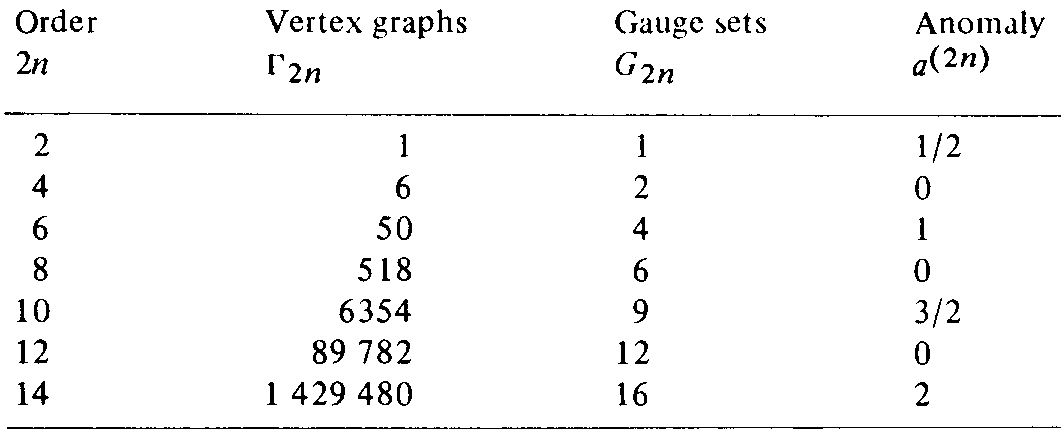
\includegraphics[width=0.80\textwidth]{../../figs/Cvit77bTab1}
\end{center}
{\scriptsize  %\caption{\label{Cvit77bTab1}
Comparison of the number of vertex diagrams without fermion loops, gauge
sets, and the ``gauge-set approximation''\footfullcite{Cvit77b} for the magnetic
moment in $2n$th order.
}
%%%%%%%%%%%%%%%%%%%%%%%%%%%%%%%%%%%%%%%%%%%%%%%%%%%%%%%%%%%
\end{frame}

\begin{frame}{Feynman's challenge, 12th Solvay Conference}
Is there any method of computing the anomalous moment of the
electron which, on first approximation, gives a fair approximation to the
$\alpha$ term and a crude one to $\alpha^2$; and when improved, increases
the accuracy of the $\alpha^2$ term, yielding a rough estimate to
$\alpha^3$ and beyond?\footfullcite{Feynman62}
\end{frame}

\begin{frame}{the unreasonable smallness of gauge sets}
%\label{sect:gaugeSetsSmall}

When the diagrams are grouped into
gauge sets,
a surprising thing happens; while the
finite part of each Feynman diagram is of order of 10 to 100,
and each one is UV and IR divergent, for $n=2,3$
every gauge set adds up to approximately
\[
		   \pm {1 \over 2} \left(\frac{\alpha}{\pi}\right)^n
\,,
\]
with the sign given by a simple empirical rule
\[
a_{kmm'} = (-1)^{m+m'}\frac{1}{2}
\] % ee{Cvit77b(5)}
\end{frame}


\begin{frame}{1977 (slightly wrong) four-loop prediction}
\begin{center}
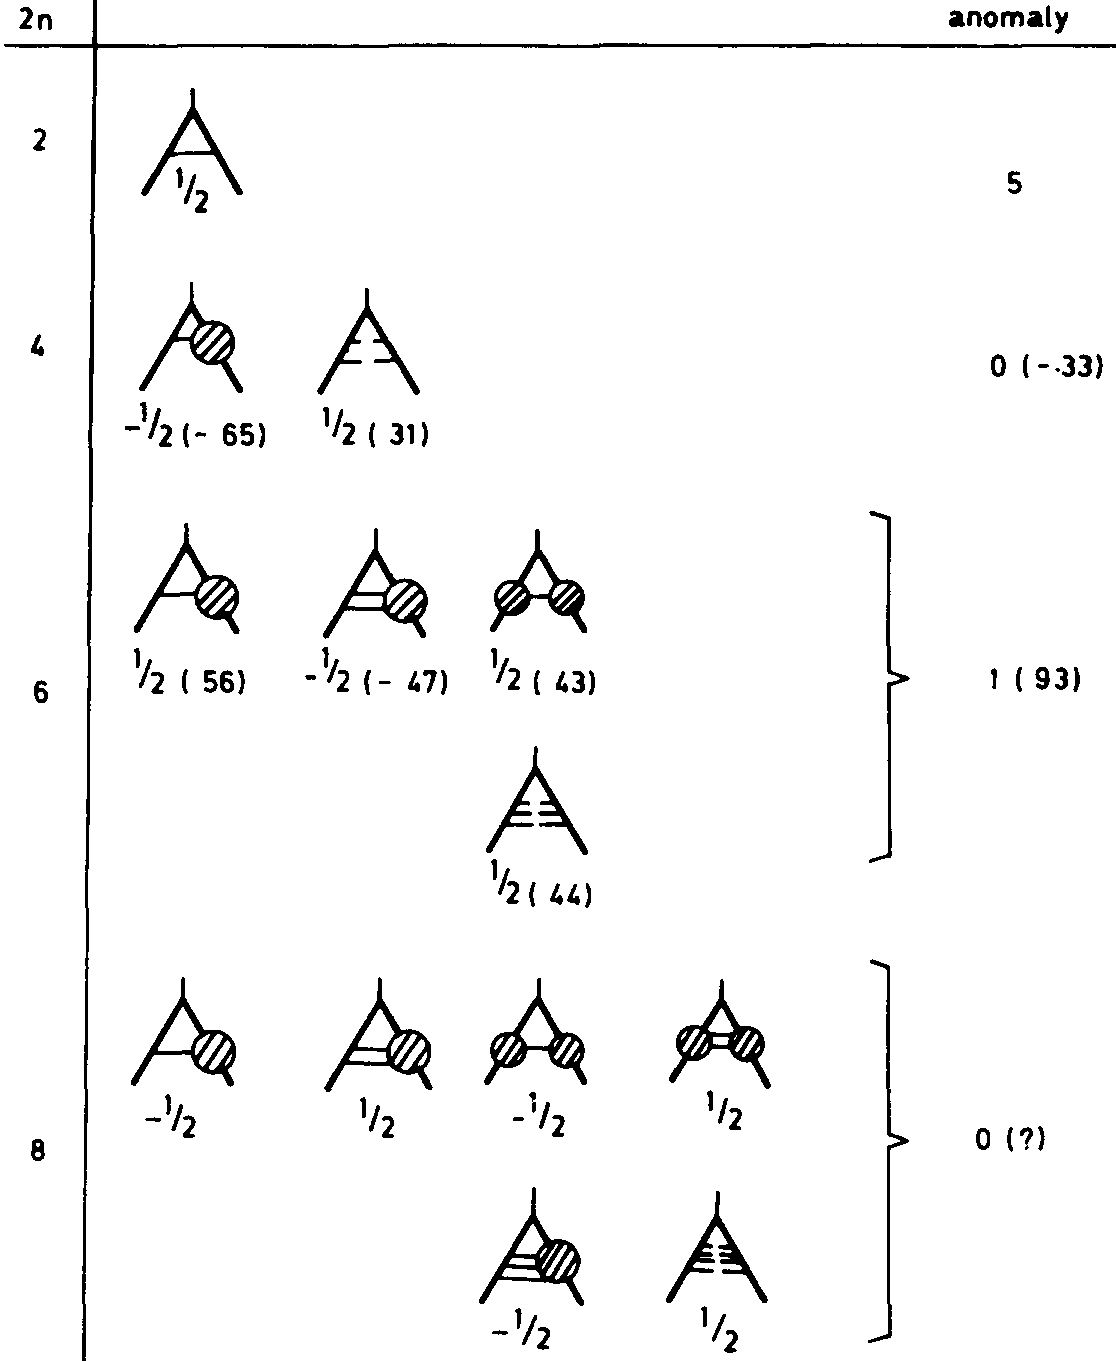
\includegraphics[width=0.50\textwidth]{Cvit77bFig3}
\end{center}

{\scriptsize  %\caption{\label{Cvit77bFig3}
new ``prediction'' : $a^{(8)}=-2$, rather than 0.
}
\end{frame}

\begin{frame}{2019 five-loop status}
%\begin
\begin{center}
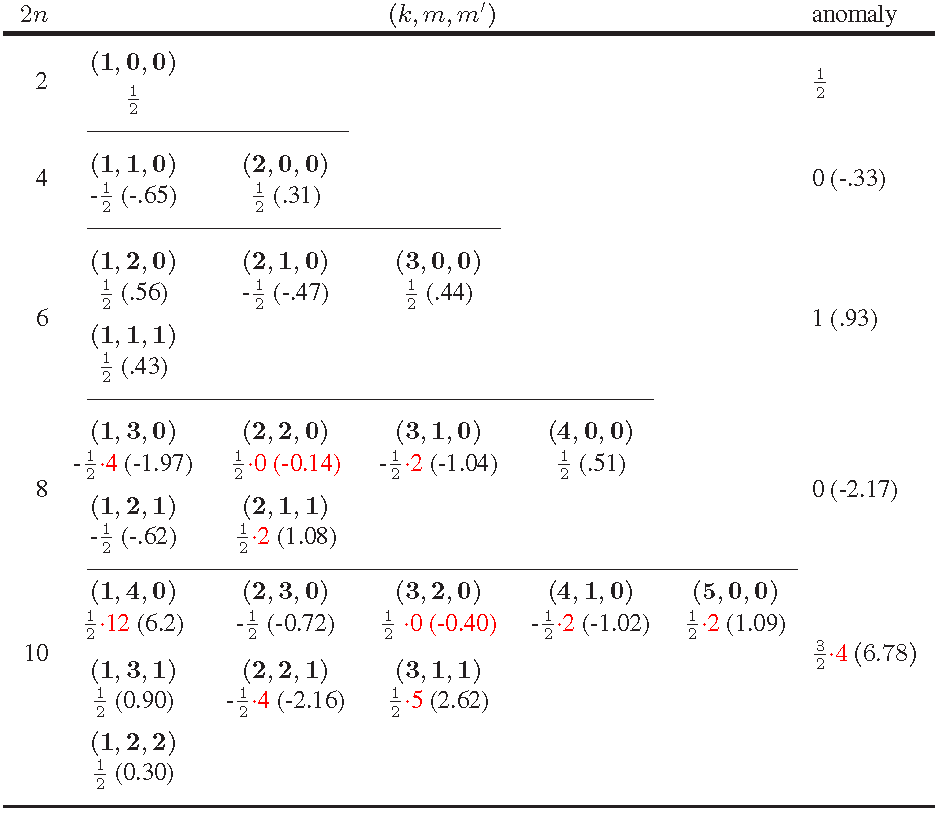
\includegraphics[width=0.65\textwidth]{finiteQEDtab1_2}
\end{center}

%\medskip

\begin{block} {gauge-set $(k,m,m')$}
{\scriptsize
[ naive ansatz $\pm\frac{1}{2}$ ] $\cdot$
[ \textcolor{red}{integer} ] $\approx$ %$\times$
[ $(\cdots)$ Volkov 2019 numerical value ]
            } % end {\scriptsize
\end{block}
\end{frame}


\begin{frame}{an example of (slightly wrong) gauge-set approximation}
With prediction \(
a_{kmm'} = (-1)^{m+m'}\!/2
\) % ee{Cvit77b(5)}
, the ``zeroth'' order estimate of the electron
magnetic moment anomaly is given by the ``gauge-set
approximation,'' convergent and summable to all orders
\[ %\beq
a=\frac{1}{2}(g-2) =  \frac{1}{2} \frac{\alpha}{\pi}
                     \frac{1}
           {\left( 1 - \left(\frac{\alpha}{\pi}\right)^2
			\right)^2
		      } + \mbox{``corrections"}
\,.
\] %ee{Cvit77b(1)}
\end{frame}

\begin{frame}{request \#3}
\begin{center}
{\huge gauge invariance matters}
\end{center}
\end{frame}


\begin{frame}{forget Dyson}
most
colleagues believe that in 1952 Dyson\footfullcite{Dyson52} had  shown that the
QED perturbation expansion is an asymptotic series (for a discussion, see
Dunne and Schubert\footfullcite{DunSch06,HuTrSc17a}), in the sense that the $n$-th order
contribution should be exploding combinatorially
$$
{1 \over 2} (g-2) \approx
\cdots + n^n \left(\frac{\alpha}{\pi}\right)^n + \cdots
\,,
$$

contrast with my estimate
\[
{1 \over 2} (g-2) \approx
\cdots + \frac{n}{2}\left(\frac{\alpha}{\pi}\right)^{2n} + \cdots
\,.
\]
hence ``QED is finite'' claim
\end{frame}

\begin{frame}{request \#4 : prove that quenched QED is finite}
\begin{center}
{\huge any bound on a gauge set, exponential or slower, will do the trick!}
\end{center}
\end{frame}

\begin{frame}{so far facts ; next, speculation with Edwards and Schubert}
\begin{enumerate}
              \item
QED finiteness conjecture
              \item {\Large
bye bye, Feynman diagrams
                  }\textcolor{gray}{\small
              \item
worldline approach
                    }
\end{enumerate}
\end{frame}


\begin{frame}{bye bye, Feynman diagrams}
it's been a good ride, but there are way too many of you
\end{frame}

\begin{frame}{a fun fact}
the idea of how to avoid Feynman diagrams can be traced to 1950 Feynman
paper\footfullcite{Feynman50}, though it took a long time for it to gain
traction

\bigskip

by the time I explained the gauge set conjecture to
him in 1975, Feynman had forgotten all about it
\end{frame}

\begin{frame}{worldline path integral for the free scalar propagator}
propagator for the Euclidean
Klein-Gordon equation\footfullcite{Schubert12} is
\[ %\beq
D_0(x,x')=\bra{x}\frac{1}{-\Box +m^2}\ket{x'}
\,,
\] %ee{Schubert12(1.1)}
exponentiate the
denominator
\[ %\beq
D_0(x,x')=\int_0^\infty\!\!dT\,{e}^{-m^2T}\bra{x}e^{-T(-\Box)}\ket{x'}
\,,
\] %ee{Schubert12(1.4)}
replace the the $D$-dimensional Laplacian by a path integral
to obtain
\[ %\beq
D_0(x,x')=\int_0^\infty\!\!dT\,e^{-m^2T}
\int_{x(0)=x'}^{x(T)=x}\!\!\!\!\mathcal{D}x(\tau)\,
    e^{-\int_0^T\!\!d\tau \frac{1}{4}\dot{x}^2}
\,,
\] %ee{Schubert12(1.7)}
\end{frame}

\begin{frame}{worldline formula for charged propagator}
that emits and reabsorbs $N$ photons as it
propagates%\footfullcite{AhBaSc16}

\medskip

Adding the QED
interaction terms leads to the Feynman's worldline path integral
representation\footfullcite{Feynman50} of the charged scalar propagator
in the presence of a background field $A(x)$,
\[ %\beq
D(x,x')=\int_0^\infty\!\!dT\,e^{-m^2T}
    \int_{x(0)=x'}^{x(T)=x}\!\!\mathcal{D}x(\tau)\,
            {e}^{-S_0-S_e-S_i}
\,,
\] %ee{AhBaSc16(1)}
where the suffix (0) indicates the free propagation
\[ %\beq
S_0 = \int_0^T\!\!d\tau \frac{1}{4}\dot{x}^2
\,,
\] %ee{Ahmadiniaz1}
(e) is the interaction of the charged scalar with the external field
\[ %\beq
S_e = -ie\int_0^T\!\!d\tau\,\dot{x}^\mu A_\mu(x(\tau))
\,,
\] %ee{Ahmadiniaz2}
\end{frame}

\begin{frame}{worldline formula for $N$-photon propagator}
and (i) are the virtual photons exchanged along the charged particle's
trajectory
\[ %\beq
S_i = \frac{e^2}{2}\int_0^T\!\!d\tau_1\int_0^T\!\!d\tau_2\,
      \dot{x}_1^\mu\,D_{\mu\nu}(x_1-x_2)\,\dot{x}_2^\nu
\,,
\] %ee{Ahmadiniaz3}
where $D_{\mu\nu} $ is the $x$-space photon propagator.

\medskip
The object of great interest to us is the internal virtual
photons term
\[ %\beq
\int_{x(0)=x'}^{x(T)=x}\!\!\mathcal{D}x(\tau)\,
            {e}^{-S_i}
=
\int_{x(0)=x'}^{x(T)=x}\!\!\mathcal{D}x(\tau)\,
            {e}^{-\frac{e^2}{2}\int_0^T\!\!d\tau_1\int_0^T\!\!d\tau_2\,
      \dot{x}_1^\mu\,D_{\mu\nu}(x_1-x_2)\,\dot{x}_2^\nu}
\] %ee{AhBaSc16(1)i}
expanded perturbatively in $\alpha/\pi$, this yields \\
the
usual $n!$ Feynman-parametric vertex diagrams
\end{frame}

\begin{frame}{worldline formalism}
however, the path integral is Gaussian in
$\dot{x}^\mu$, and if by integration by parts, $\dot{x}^\mu$ are
eliminated in favor of $x^\mu$, internal photons can be integrated over
directly, prior to an expansion in $(\alpha/\pi)^n$, and one gets
integrals in terms of

\begin{block}{$N$-photon propagators}
symmetrized sums over $N$ photons
\end{block}
and not the usual
Feynman graphs

\bigskip
each usual Feynman graph corresponds to one particular
permutation of internal photon insertions, and from that comes the
factorial growth in the number of graphs
\end{frame}

\begin{frame}{worldline formalism}
note : the worldline integrals are expressed
in terms of $N$-photon propagators, \\
the central ingredient that defines
the \textcolor{red!80!black}{gauge sets}

\bigskip
unlike the Feynman parameter integrals for individual vertex graphs, they are
independent of the ordering of the momenta $k_1,\ldots,k_N$; the worline formula
contains all $\approx N!$ ways of attaching the $N$ internal
photons to the charged particle propagator

\bigskip
worldline representation combines
\\
\textcolor{green!80!black}{combinatorially many} Feynman diagrams into

\medskip\hfill
a \textcolor{green!80!black}{{\Huge single}} integral

\end{frame}

\begin{frame}{worldline formalism}
In QED the $N$-photon propagator formulation combines into one integral
all Feynman graphs related by permutations of photon legs along fermion
lines, that is, it yield a \emph{single} integral for a gauge set
$kmm'$
\end{frame}

\begin{frame}{worldline formalism}
\begin{center}
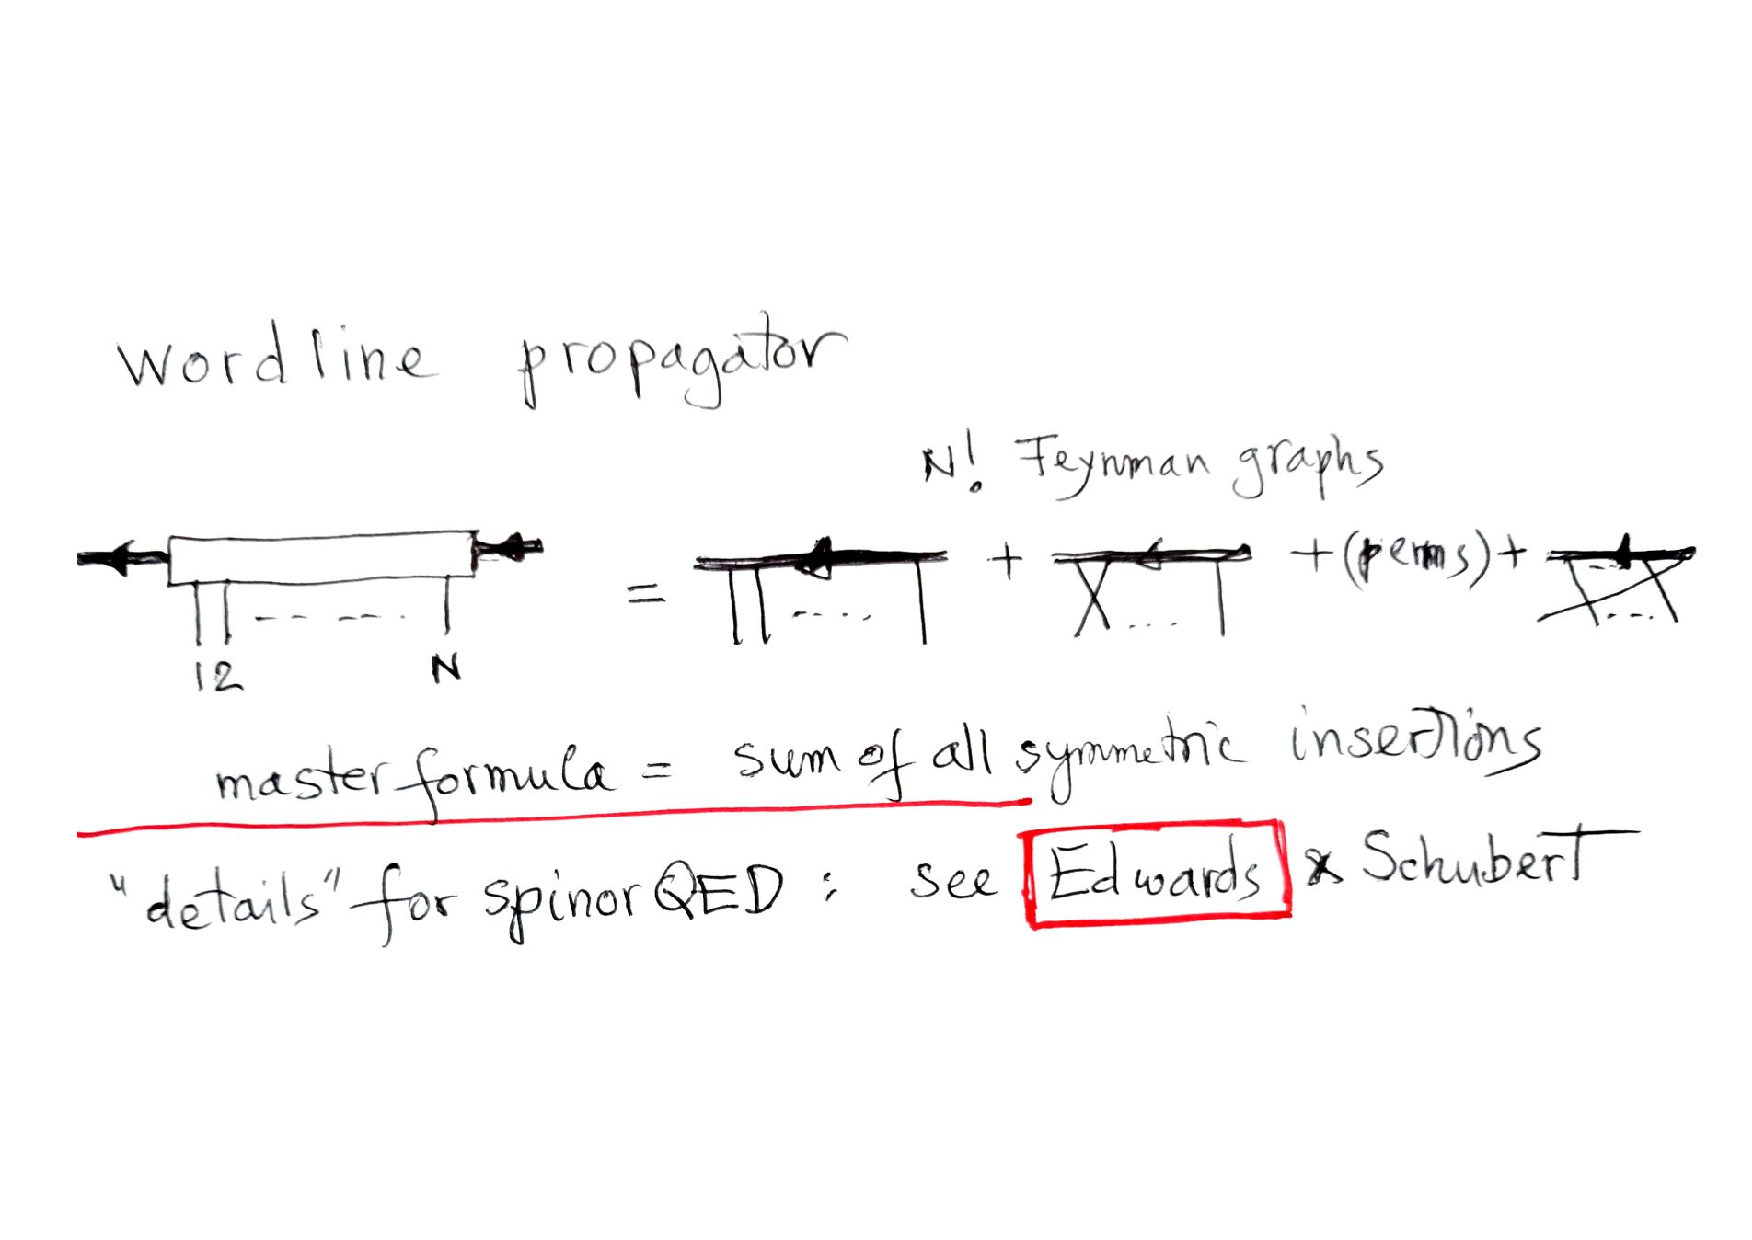
\includegraphics[width=0.90\textwidth]{worldlinProp}
\end{center}
\end{frame}
\begin{frame}{worldline formalism}
\begin{center}
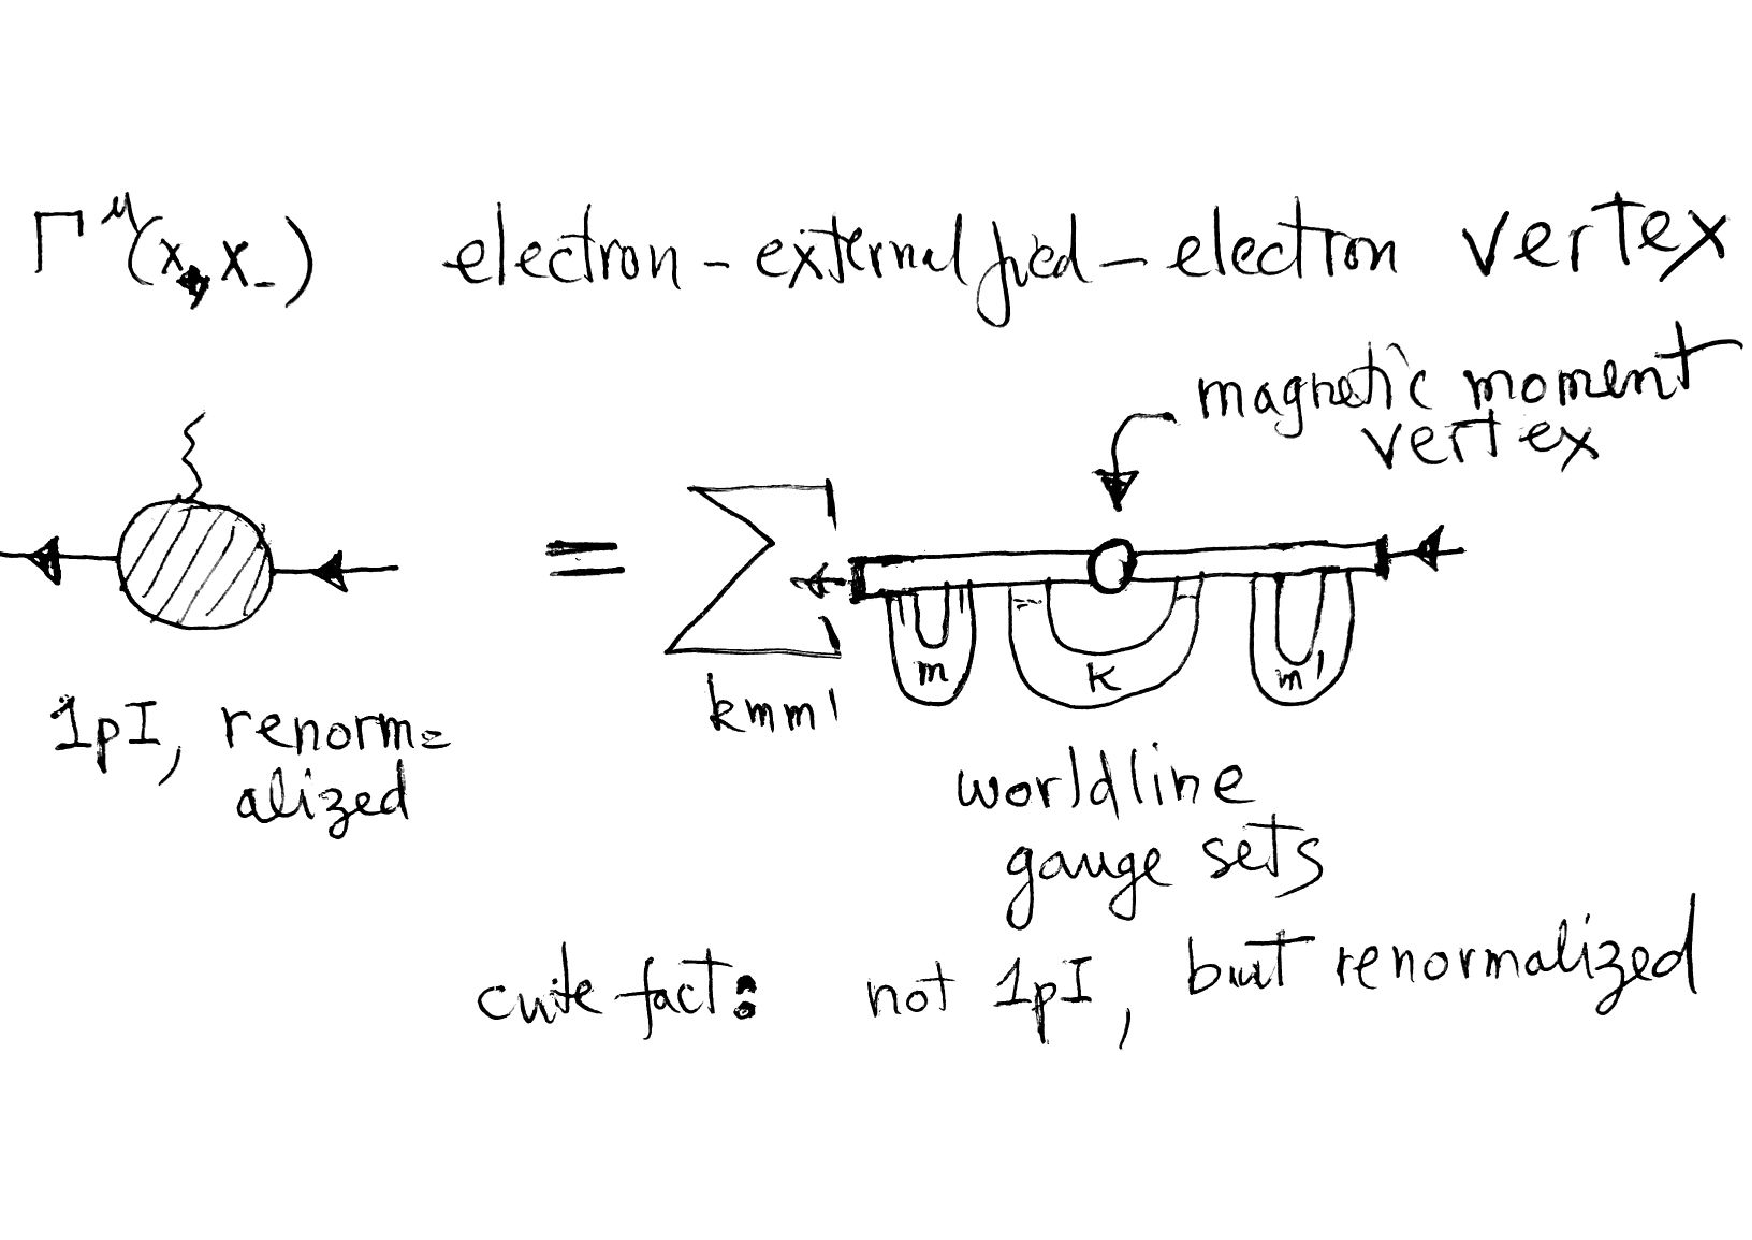
\includegraphics[width=0.90\textwidth]{worldlineGsets}
\end{center}
\end{frame}
\begin{frame}{worldline formalism}
\begin{center}
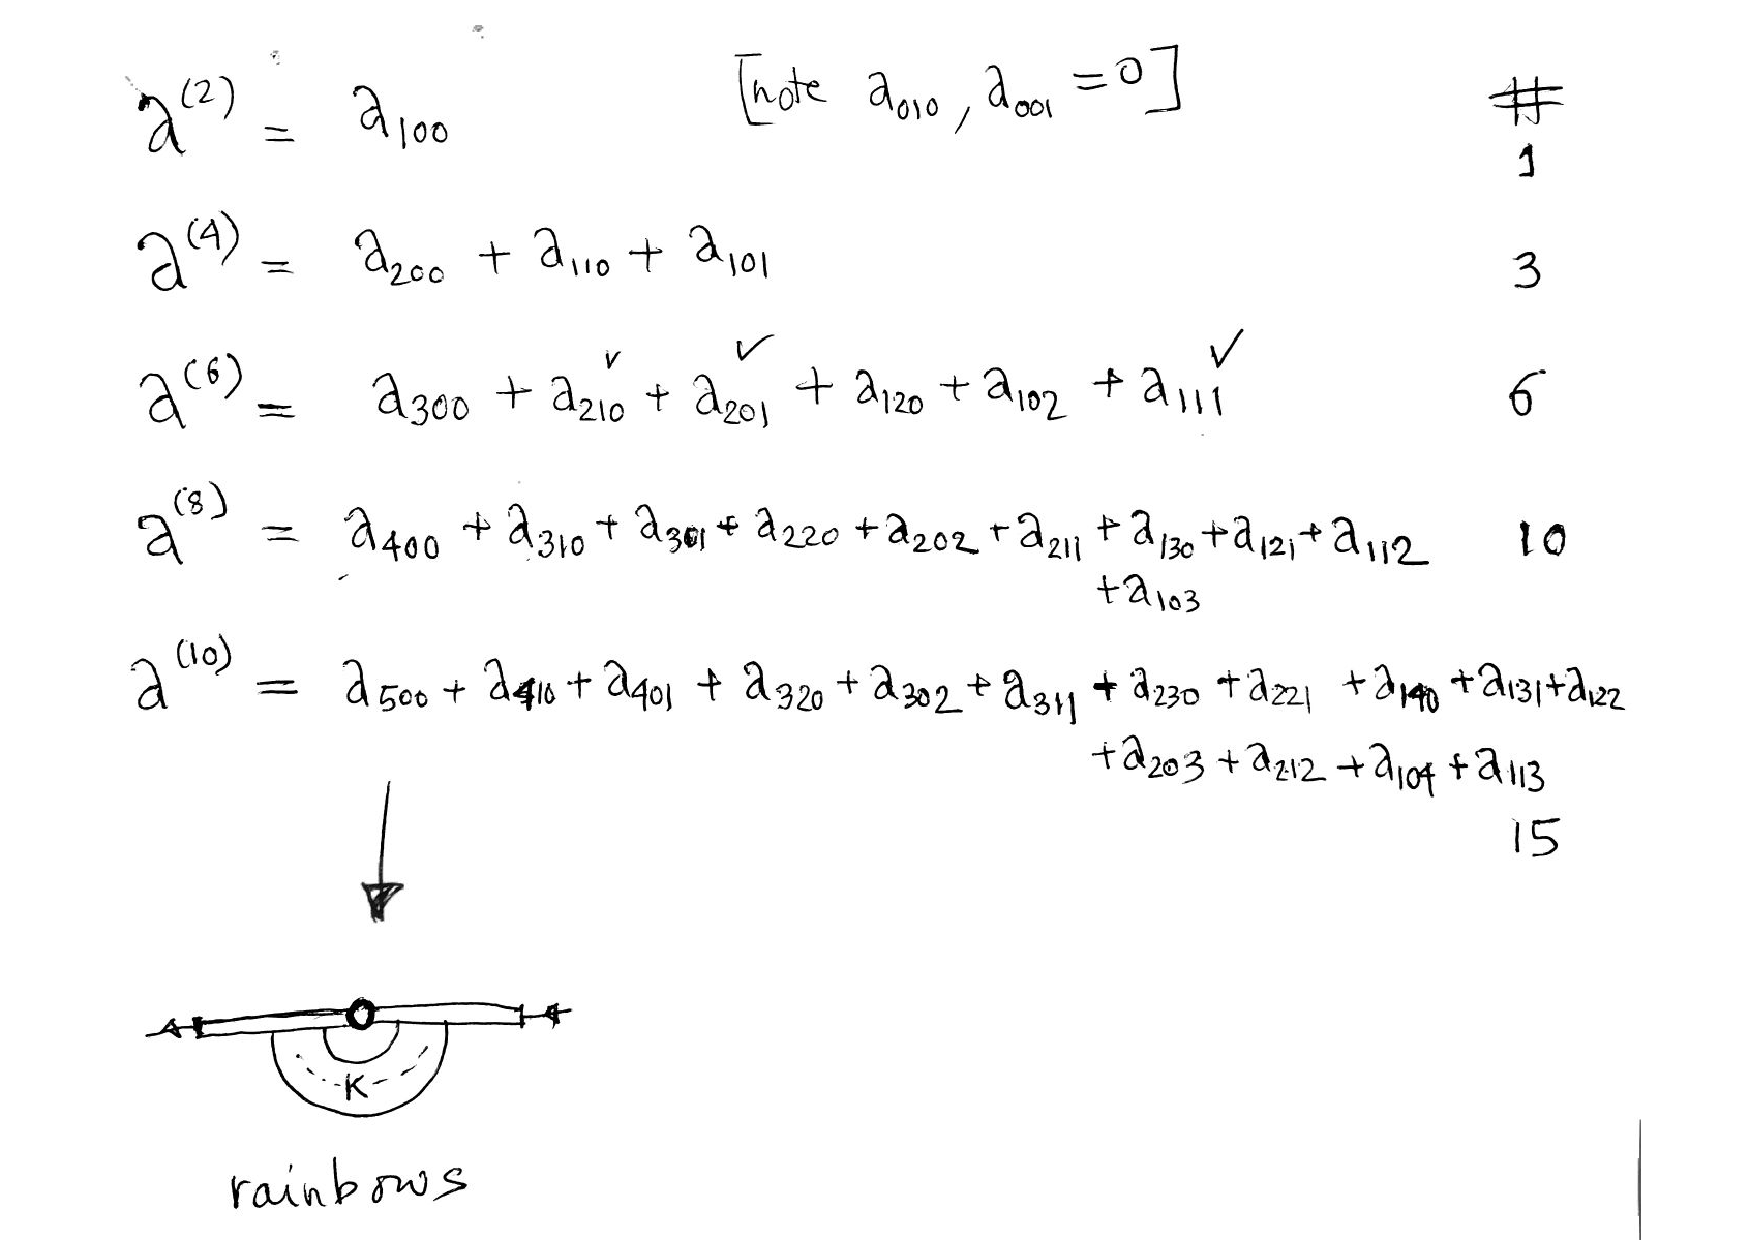
\includegraphics[width=0.50\textwidth]{gaugeSets}
\end{center}
\end{frame}
\begin{frame}{worldline formalism}
\begin{center}
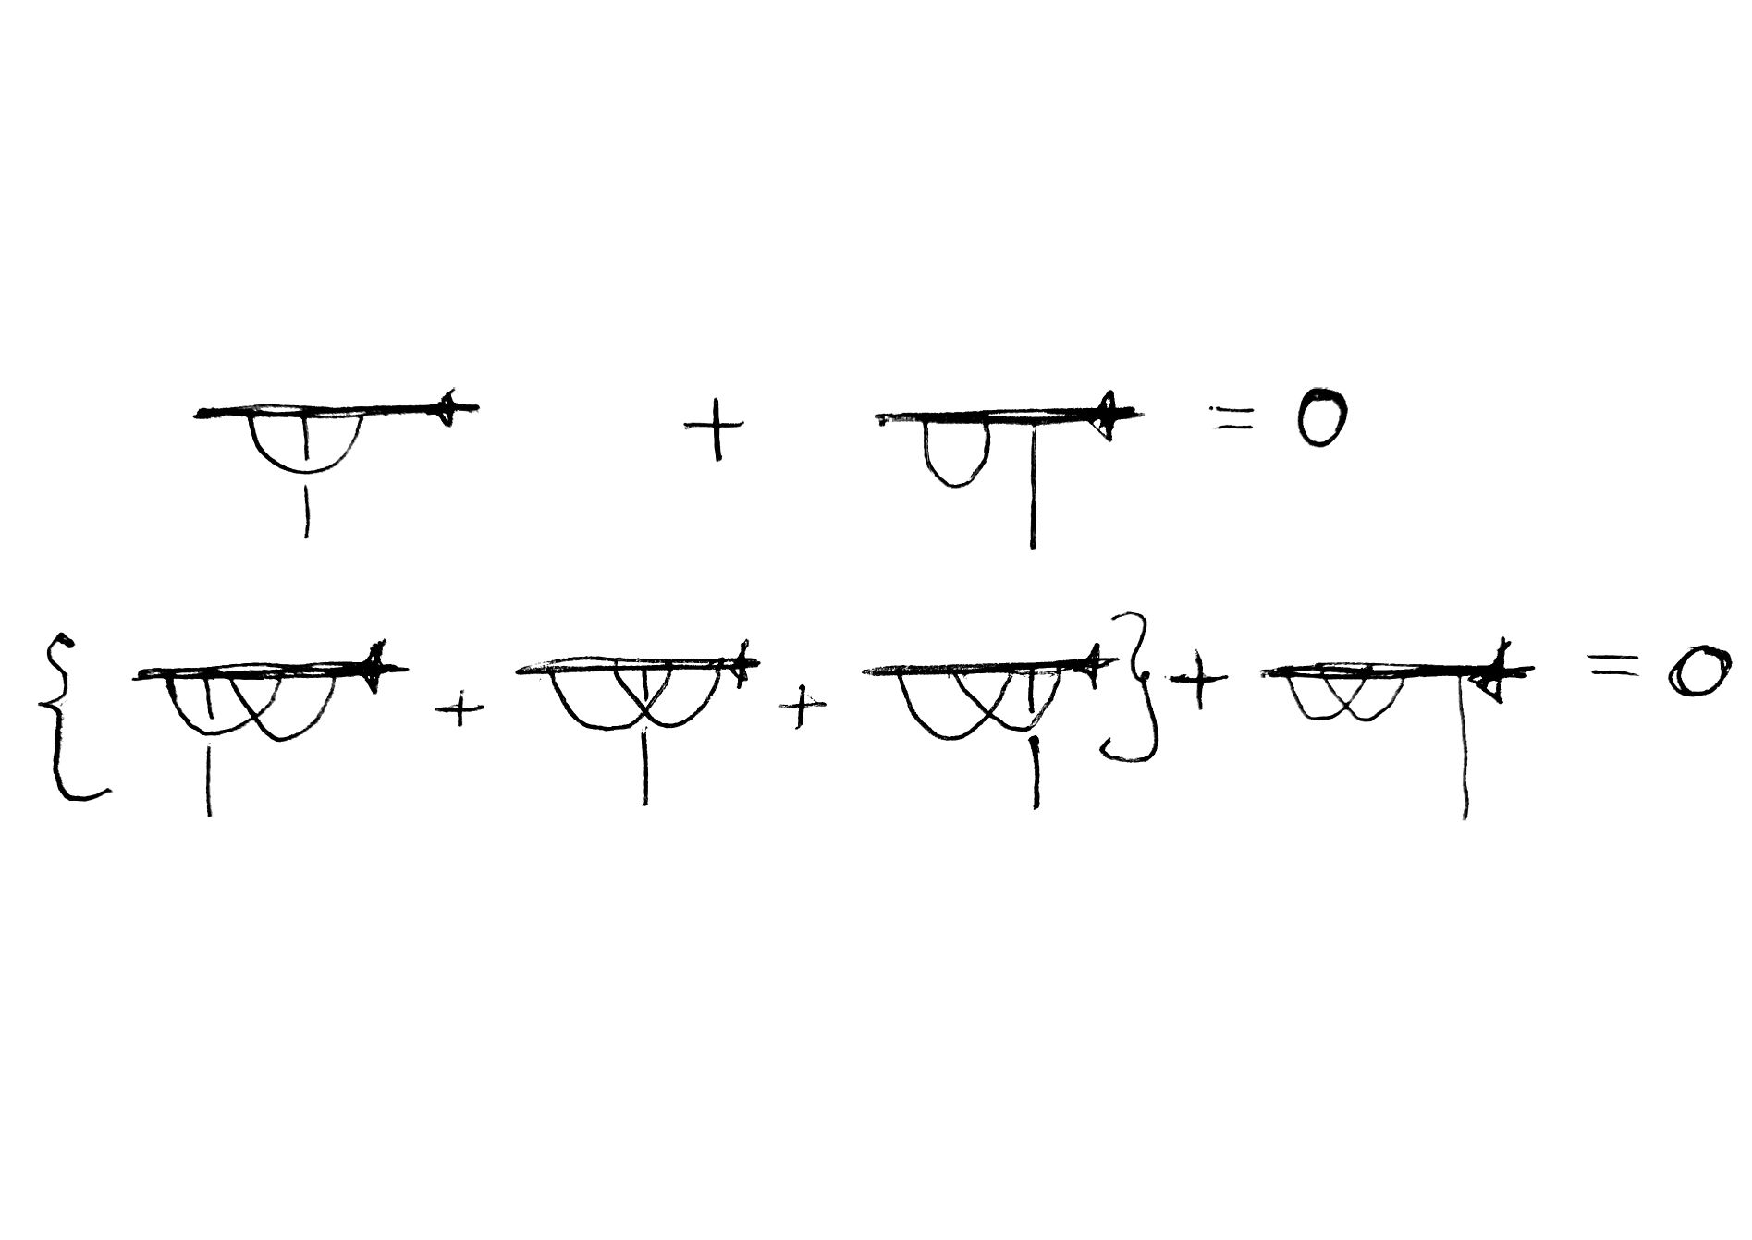
\includegraphics[width=0.90\textwidth]{WardIds}
\end{center}
\end{frame}
\begin{frame}{worldline formalism}
\begin{center}
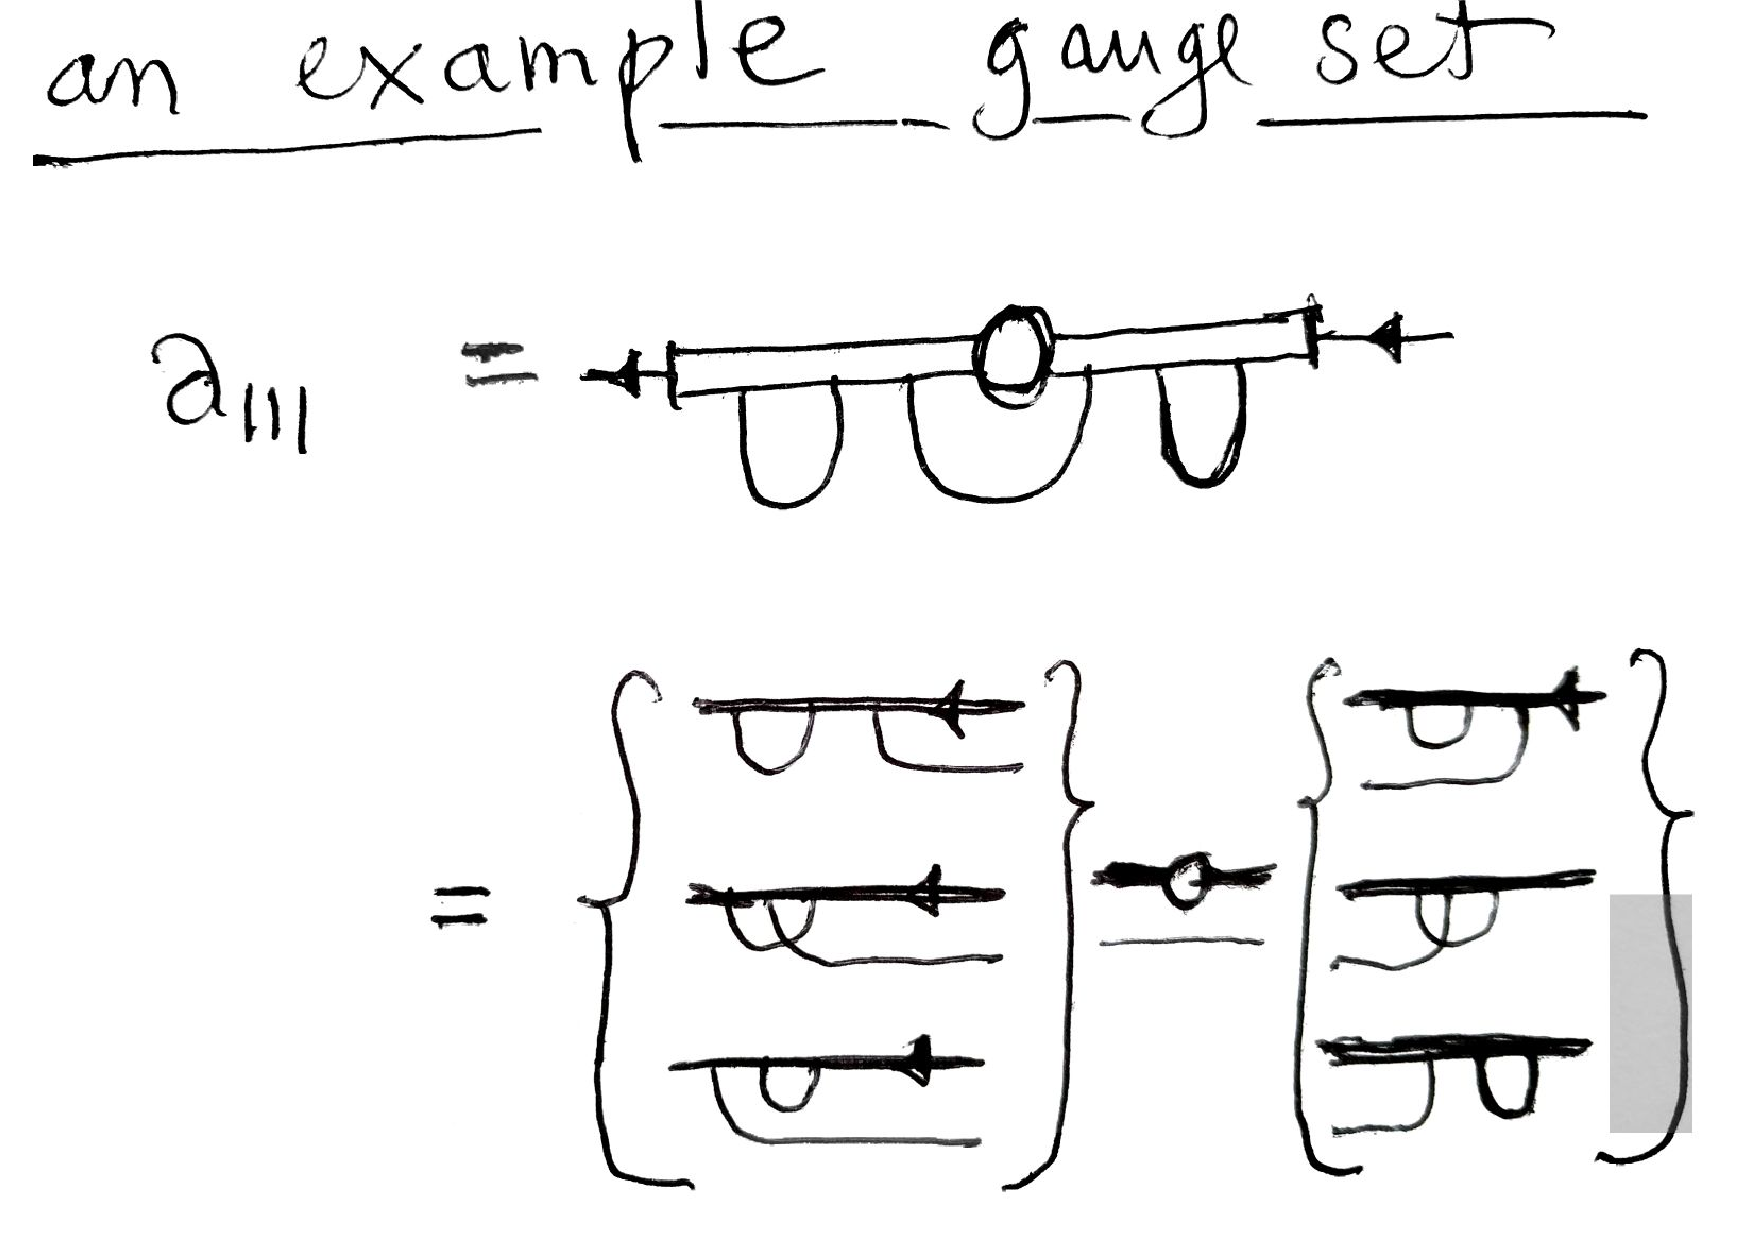
\includegraphics[width=0.90\textwidth]{a111a}
\end{center}
\end{frame}
\begin{frame}{worldline formalism}
\begin{center}
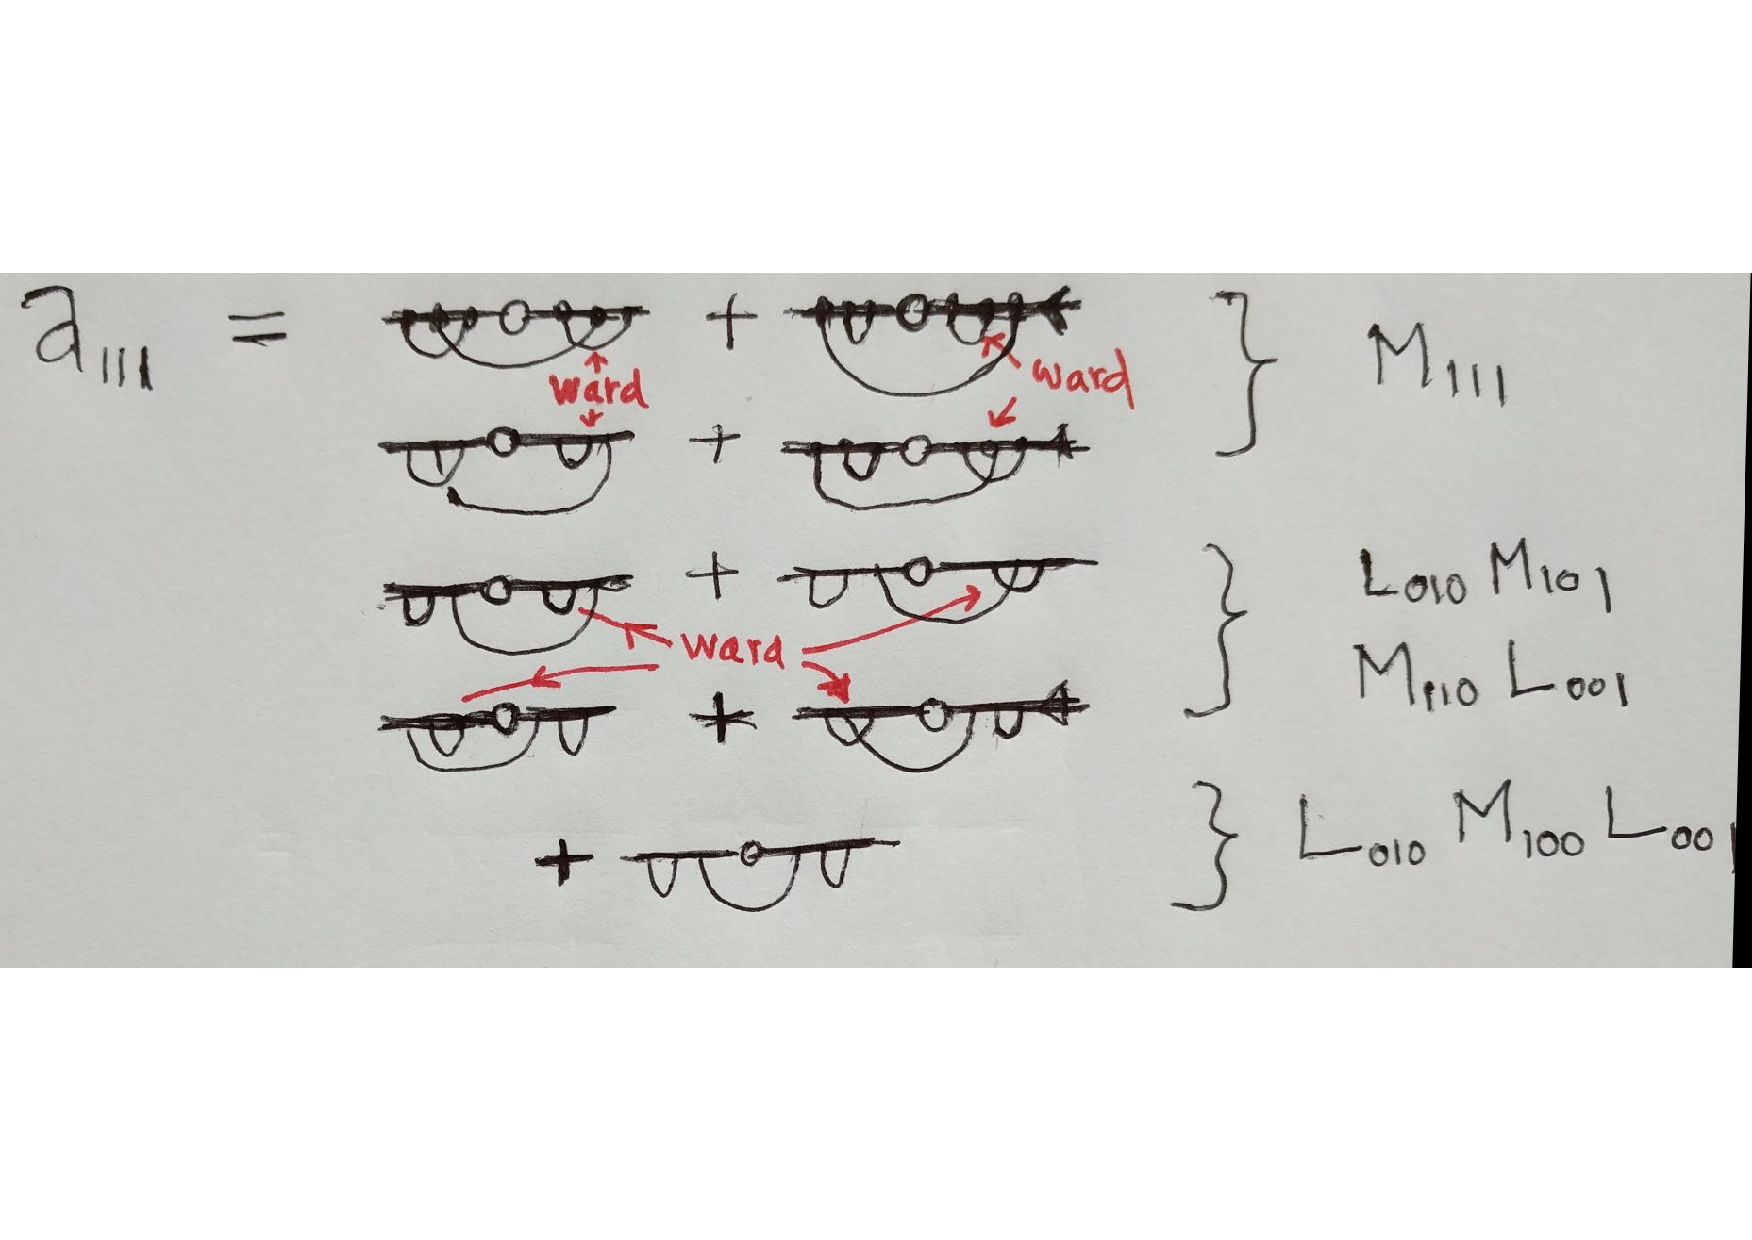
\includegraphics[width=0.90\textwidth]{a111b}
\end{center}
\end{frame}

\begin{frame}{summary}
\begin{enumerate}
              \item
a proof of the QED finiteness conjecture might be within reach

              \item
so might be methods for computing gauge invariant QFT sets without
recourse to Feynman diagrams

\end{enumerate}

\vfill
\bigskip\noindent{\scriptsize
you can download the current version of full notes here:
\HREF{http://chaosbook.org/~predrag/papers/finiteQED.pdf}
{ChaosBook.org/$\sim$predrag/papers/finiteQED.pdf}
\\The source code:
\HREF{https://GitHub.com/cvitanov/reducesymm/QFT}
{GitHub.com/cvitanov/reducesymm/QFT}
            }
\end{frame}



\end{document}

    \newpage
    % reducesymm/QFT/correspnd.tex
% $Author$ $Date$
% Predrag  switched to github.com               jul  8 2013

\section{Is QED finite? Correspondence}
\label{sect:correspnd}


\begin{bartlett}{
I am not sure I'll will tell you anything useful any time soon, as I'm a
lapsed field theorist, but here is for your amusement my
\HREF{https://vimeo.com/79605418} {recent rant}. To
cite my wife: ``You may well be right".
        }
\bauthor{
\HREF{http://www.goodreads.com/work/quotes/3226250-keep-the-aspidistra-flying}
{Keep the Aspidistra Flying!}
    }
\end{bartlett}
\bigskip



\begin{description}

\item[2007-03-18 Dirk Kreimer] % kreimer@ihes.fr via nbi.dk
I was pretty much looking forward to grab you for a chat on Dyson
Schwinger etc whilst in Bonn this starting week. Now I fail to be there
myself due to a stupid mechanical problem with a vertebrae.
Pondering about other options, let me just point out that the IHES
(www.ihes.fr) has an excellent visitor program. If you foresee some time
you fancy to pay us a visit, please go ahead.

I am running a little seminar at Boston whilst being there, so besides
what works out with IHES,  whenever you are available in the above
period, you are herewith invited for a talk at BU.
Would you be able to come for a seminar to Boston, Thu, Nov 29 this year?

\item[2011-08-23 Predrag] to Dirk:

I feel like some stuck-up god knows who for not having answered sooner -
but it is not that. I have been focusing on turbulence (with the goal of
using what I learn on Yang-Mills, eventually - if it works, Feynman
diagrammar will be of secondary importance, the first step is fully and
totally non-perturbative) so I feel like fraud talking about QFT when I
am suspended between the perturbative past and the elusive
non-perturbative future.

If someone wants to hear about turbulence as in
\HREF{http://ChaosBook.org/tutorials} {ChaosBook.org/tutorials}, I can do
that honestly - otherwise we wait until I actually do any QFT worth
hearing about...

I got \HREF{http://birdtracks.eu} {birdtracks.eu} published, finally -
you get 100 birdtracks per 1\$, a real deal if you are into that kind of
thing.

Guilty as Charged -
Predrag

\item[2011-08-26 Dirk]
June 01-05 2009 I am organizing a workshop at IHES. It has a
non-perturbative component via Dyson--Schwinger eqs. Would you be
interested to participate and come?

\item[2017-06-16 Dirk]
I will show your notes to
Henry Ki{\ss}ler\rf{Kissler16}   <kissler@physik.hu-berlin.de>
and
\HREF{http://people.physik.hu-berlin.de/~borinsky/}
{Michael Borinsky}\rf{Borinsky14,Borinsky17}    <borinsky@physik.hu-berlin.de> .

There should be a few people at Les Houches June 2018 who have something
to say about asymptotics of solutions of Dyson-Schwinger equation for
example.


\end{description}

%% Laporta17figuragau.tex %%%%%
%% compiled by  reducesymm/QFT/blog.tex
%%%%%%%%%%%%%%%%%%%%%%%%%%%%%%%%%%%%%%%%
\begin{figure}
\begin{center}
\begin{picture}(125,325)(70,50)
\thicklines
%%%
{
\put(+000.0,+200.0){\makebox(0,0)[lb]{
% fotone obliquo (0.000000,200.000000) (0.000000,205.000000)
   \qbezier(+000.0,+200.0)(+001.2,+201.2)(+000.0,+202.5)
   \qbezier(+000.0,+202.5)(-001.2,+203.8)(+000.0,+205.0)
% elettrone curvo (0.000000,200.000000) (-20.000000,160.000000) 1000.000000
% cerchio r=44721.365140 c=(-40010.000000,20180.000000) ang=(-26.536403,-26.593699)
   \qbezier(+000.0,+200.0)(-010.0,+180.0)(-020.0,+160.0)
% elettrone curvo (0.000000,200.000000) (20.000000,160.000000) 1000.000000
% cerchio r=44721.365140 c=(-39990.000000,-19820.000000) ang=(26.593699,26.536403)
   \qbezier(+000.0,+200.0)(+010.0,+180.0)(+020.0,+160.0)
% fotone obliquo (-14.142136,171.715729) (14.142136,171.715729)
   \qbezier(-014.1,+171.7)(-013.3,+170.8)(-012.4,+171.7)
   \qbezier(-012.4,+171.7)(-011.5,+172.6)(-010.6,+171.7)
   \qbezier(-010.6,+171.7)(-009.7,+170.8)(-008.8,+171.7)
   \qbezier(-008.8,+171.7)(-008.0,+172.6)(-007.1,+171.7)
   \qbezier(-007.1,+171.7)(-006.2,+170.8)(-005.3,+171.7)
   \qbezier(-005.3,+171.7)(-004.4,+172.6)(-003.5,+171.7)
   \qbezier(-003.5,+171.7)(-002.7,+170.8)(-001.8,+171.7)
   \qbezier(-001.8,+171.7)(-000.9,+172.6)(+000.0,+171.7)
   \qbezier(+000.0,+171.7)(+000.9,+170.8)(+001.8,+171.7)
   \qbezier(+001.8,+171.7)(+002.7,+172.6)(+003.5,+171.7)
   \qbezier(+003.5,+171.7)(+004.4,+170.8)(+005.3,+171.7)
   \qbezier(+005.3,+171.7)(+006.2,+172.6)(+007.1,+171.7)
   \qbezier(+007.1,+171.7)(+008.0,+170.8)(+008.8,+171.7)
   \qbezier(+008.8,+171.7)(+009.7,+172.6)(+010.6,+171.7)
   \qbezier(+010.6,+171.7)(+011.5,+170.8)(+012.4,+171.7)
   \qbezier(+012.4,+171.7)(+013.3,+172.6)(+014.1,+171.7)
% fotone curvo (5.303301,189.393398) (10.000000,180.000000) 0.100000
% fotone semicircolare r=5.355061 c=(6.712311,184.227029) ang=(105.255119,-52.125016)
% n=8
   \qbezier(+005.3,+189.4)(+006.3,+188.7)(+007.1,+189.6)
   \qbezier(+007.1,+189.6)(+008.3,+190.3)(+008.9,+189.1)
   \qbezier(+008.9,+189.1)(+009.2,+187.9)(+010.4,+188.1)
   \qbezier(+010.4,+188.1)(+011.7,+187.9)(+011.5,+186.6)
   \qbezier(+011.5,+186.6)(+011.0,+185.5)(+012.0,+184.9)
   \qbezier(+012.0,+184.9)(+013.0,+183.9)(+011.9,+183.0)
   \qbezier(+011.9,+183.0)(+010.8,+182.5)(+011.2,+181.4)
   \qbezier(+011.2,+181.4)(+011.3,+180.0)(+010.0,+180.0)
% fotone curvo (12.247449,175.505103) (17.320508,165.358984) 0.100000
% fotone semicircolare r=5.784178 c=(13.769367,169.924737) ang=(105.255119,-52.125016)
% n=9
   \qbezier(+012.2,+175.5)(+013.2,+174.8)(+014.0,+175.7)
   \qbezier(+014.0,+175.7)(+015.0,+176.5)(+015.7,+175.4)
   \qbezier(+015.7,+175.4)(+016.1,+174.2)(+017.3,+174.5)
   \qbezier(+017.3,+174.5)(+018.6,+174.6)(+018.5,+173.3)
   \qbezier(+018.5,+173.3)(+018.2,+172.1)(+019.3,+171.7)
   \qbezier(+019.3,+171.7)(+020.3,+171.0)(+019.6,+170.0)
   \qbezier(+019.6,+170.0)(+018.6,+169.2)(+019.3,+168.2)
   \qbezier(+019.3,+168.2)(+019.8,+167.0)(+018.5,+166.6)
   \qbezier(+018.5,+166.6)(+017.3,+166.5)(+017.3,+165.4)
% fotone curvo (15.811388,168.377223) (18.708287,162.583426) -0.100000
% fotone semicircolare r=3.302973 c=(17.839217,165.770015) ang=(127.874984,285.255119)
% n=5
   \qbezier(+015.8,+168.4)(+014.5,+168.2)(+014.7,+166.9)
   \qbezier(+014.7,+166.9)(+015.4,+166.0)(+014.6,+165.1)
   \qbezier(+014.6,+165.1)(+014.1,+163.9)(+015.4,+163.5)
   \qbezier(+015.4,+163.5)(+016.5,+163.7)(+016.9,+162.6)
   \qbezier(+016.9,+162.6)(+017.8,+161.6)(+018.7,+162.6)
\put(+000.0,+152.0){\makebox(0,0){$(1)$}}
}}
\put(+025.0,+200.0){\makebox(0,0)[lb]{
% fotone obliquo (25.000000,200.000000) (25.000000,205.000000)
   \qbezier(+025.0,+200.0)(+026.2,+201.2)(+025.0,+202.5)
   \qbezier(+025.0,+202.5)(+023.8,+203.8)(+025.0,+205.0)
% elettrone curvo (25.000000,200.000000) (5.000000,160.000000) 1000.000000
% cerchio r=44721.365140 c=(-39985.000000,20180.000000) ang=(-26.536403,-26.593699)
   \qbezier(+025.0,+200.0)(+015.0,+180.0)(+005.0,+160.0)
% elettrone curvo (25.000000,200.000000) (45.000000,160.000000) 1000.000000
% cerchio r=44721.365140 c=(-39965.000000,-19820.000000) ang=(26.593699,26.536403)
   \qbezier(+025.0,+200.0)(+035.0,+180.0)(+045.0,+160.0)
% fotone obliquo (14.309550,178.619101) (35.690450,178.619101)
   \qbezier(+014.3,+178.6)(+015.2,+177.7)(+016.1,+178.6)
   \qbezier(+016.1,+178.6)(+017.0,+179.5)(+017.9,+178.6)
   \qbezier(+017.9,+178.6)(+018.8,+177.7)(+019.7,+178.6)
   \qbezier(+019.7,+178.6)(+020.5,+179.5)(+021.4,+178.6)
   \qbezier(+021.4,+178.6)(+022.3,+177.7)(+023.2,+178.6)
   \qbezier(+023.2,+178.6)(+024.1,+179.5)(+025.0,+178.6)
   \qbezier(+025.0,+178.6)(+025.9,+177.7)(+026.8,+178.6)
   \qbezier(+026.8,+178.6)(+027.7,+179.5)(+028.6,+178.6)
   \qbezier(+028.6,+178.6)(+029.5,+177.7)(+030.3,+178.6)
   \qbezier(+030.3,+178.6)(+031.2,+179.5)(+032.1,+178.6)
   \qbezier(+032.1,+178.6)(+033.0,+177.7)(+033.9,+178.6)
   \qbezier(+033.9,+178.6)(+034.8,+179.5)(+035.7,+178.6)
% fotone obliquo (8.096915,166.193830) (41.903085,166.193830)
   \qbezier(+008.1,+166.2)(+009.0,+165.3)(+009.9,+166.2)
   \qbezier(+009.9,+166.2)(+010.8,+167.1)(+011.7,+166.2)
   \qbezier(+011.7,+166.2)(+012.5,+165.3)(+013.4,+166.2)
   \qbezier(+013.4,+166.2)(+014.3,+167.1)(+015.2,+166.2)
   \qbezier(+015.2,+166.2)(+016.1,+165.3)(+017.0,+166.2)
   \qbezier(+017.0,+166.2)(+017.9,+167.1)(+018.8,+166.2)
   \qbezier(+018.8,+166.2)(+019.7,+165.3)(+020.6,+166.2)
   \qbezier(+020.6,+166.2)(+021.4,+167.1)(+022.3,+166.2)
   \qbezier(+022.3,+166.2)(+023.2,+165.3)(+024.1,+166.2)
   \qbezier(+024.1,+166.2)(+025.0,+167.1)(+025.9,+166.2)
   \qbezier(+025.9,+166.2)(+026.8,+165.3)(+027.7,+166.2)
   \qbezier(+027.7,+166.2)(+028.6,+167.1)(+029.4,+166.2)
   \qbezier(+029.4,+166.2)(+030.3,+165.3)(+031.2,+166.2)
   \qbezier(+031.2,+166.2)(+032.1,+167.1)(+033.0,+166.2)
   \qbezier(+033.0,+166.2)(+033.9,+165.3)(+034.8,+166.2)
   \qbezier(+034.8,+166.2)(+035.7,+167.1)(+036.6,+166.2)
   \qbezier(+036.6,+166.2)(+037.5,+165.3)(+038.3,+166.2)
   \qbezier(+038.3,+166.2)(+039.2,+167.1)(+040.1,+166.2)
   \qbezier(+040.1,+166.2)(+041.0,+165.3)(+041.9,+166.2)
% fotone curvo (32.559289,184.881421) (38.093073,173.813853) 0.100000
% fotone semicircolare r=6.309484 c=(34.219425,178.794259) ang=(105.255119,-52.125016)
% n=9
   \qbezier(+032.6,+184.9)(+033.6,+184.1)(+034.5,+185.1)
   \qbezier(+034.5,+185.1)(+035.6,+185.9)(+036.3,+184.7)
   \qbezier(+036.3,+184.7)(+036.8,+183.5)(+038.0,+183.8)
   \qbezier(+038.0,+183.8)(+039.4,+183.8)(+039.4,+182.4)
   \qbezier(+039.4,+182.4)(+039.0,+181.2)(+040.2,+180.7)
   \qbezier(+040.2,+180.7)(+041.4,+179.9)(+040.5,+178.8)
   \qbezier(+040.5,+178.8)(+039.5,+178.0)(+040.2,+176.9)
   \qbezier(+040.2,+176.9)(+040.7,+175.6)(+039.4,+175.2)
   \qbezier(+039.4,+175.2)(+038.1,+175.1)(+038.1,+173.8)
% fotone curvo (40.118579,169.762842) (43.516402,162.967196) 0.100000
% fotone semicircolare r=3.874114 c=(41.137926,166.025237) ang=(105.255119,-52.125016)
% n=6
   \qbezier(+040.1,+169.8)(+041.0,+169.0)(+041.9,+169.8)
   \qbezier(+041.9,+169.8)(+043.1,+170.3)(+043.5,+169.1)
   \qbezier(+043.5,+169.1)(+043.5,+168.0)(+044.6,+167.8)
   \qbezier(+044.6,+167.8)(+045.7,+167.1)(+045.0,+166.0)
   \qbezier(+045.0,+166.0)(+044.1,+165.4)(+044.6,+164.3)
   \qbezier(+044.6,+164.3)(+044.8,+163.0)(+043.5,+163.0)
\put(+025.0,+152.0){\makebox(0,0){$(2)$}}
}}
\put(+050.0,+200.0){\makebox(0,0)[lb]{
% fotone obliquo (50.000000,200.000000) (50.000000,205.000000)
   \qbezier(+050.0,+200.0)(+051.2,+201.2)(+050.0,+202.5)
   \qbezier(+050.0,+202.5)(+048.8,+203.8)(+050.0,+205.0)
% elettrone curvo (50.000000,200.000000) (30.000000,160.000000) 1000.000000
% cerchio r=44721.365140 c=(-39960.000000,20180.000000) ang=(-26.536403,-26.593699)
   \qbezier(+050.0,+200.0)(+040.0,+180.0)(+030.0,+160.0)
% elettrone curvo (50.000000,200.000000) (70.000000,160.000000) 1000.000000
% cerchio r=44721.365140 c=(-39940.000000,-19820.000000) ang=(26.593699,26.536403)
   \qbezier(+050.0,+200.0)(+060.0,+180.0)(+070.0,+160.0)
% fotone obliquo (33.670068,167.340137) (66.329932,167.340137)
   \qbezier(+033.7,+167.3)(+034.5,+166.5)(+035.4,+167.3)
   \qbezier(+035.4,+167.3)(+036.2,+168.2)(+037.1,+167.3)
   \qbezier(+037.1,+167.3)(+038.0,+166.5)(+038.8,+167.3)
   \qbezier(+038.8,+167.3)(+039.7,+168.2)(+040.5,+167.3)
   \qbezier(+040.5,+167.3)(+041.4,+166.5)(+042.3,+167.3)
   \qbezier(+042.3,+167.3)(+043.1,+168.2)(+044.0,+167.3)
   \qbezier(+044.0,+167.3)(+044.8,+166.5)(+045.7,+167.3)
   \qbezier(+045.7,+167.3)(+046.6,+168.2)(+047.4,+167.3)
   \qbezier(+047.4,+167.3)(+048.3,+166.5)(+049.1,+167.3)
   \qbezier(+049.1,+167.3)(+050.0,+168.2)(+050.9,+167.3)
   \qbezier(+050.9,+167.3)(+051.7,+166.5)(+052.6,+167.3)
   \qbezier(+052.6,+167.3)(+053.4,+168.2)(+054.3,+167.3)
   \qbezier(+054.3,+167.3)(+055.2,+166.5)(+056.0,+167.3)
   \qbezier(+056.0,+167.3)(+056.9,+168.2)(+057.7,+167.3)
   \qbezier(+057.7,+167.3)(+058.6,+166.5)(+059.5,+167.3)
   \qbezier(+059.5,+167.3)(+060.3,+168.2)(+061.2,+167.3)
   \qbezier(+061.2,+167.3)(+062.0,+166.5)(+062.9,+167.3)
   \qbezier(+062.9,+167.3)(+063.8,+168.2)(+064.6,+167.3)
   \qbezier(+064.6,+167.3)(+065.5,+166.5)(+066.3,+167.3)
% fotone curvo (35.857864,171.715729) (31.742581,163.485163) -0.100000
% fotone semicircolare r=4.692144 c=(34.623279,167.188917) ang=(74.744881,232.125016)
% n=7
   \qbezier(+035.9,+171.7)(+035.0,+172.8)(+034.0,+171.8)
   \qbezier(+034.0,+171.8)(+033.4,+170.8)(+032.3,+171.3)
   \qbezier(+032.3,+171.3)(+031.0,+171.4)(+030.9,+170.1)
   \qbezier(+030.9,+170.1)(+031.2,+168.9)(+030.1,+168.4)
   \qbezier(+030.1,+168.4)(+029.0,+167.6)(+030.0,+166.6)
   \qbezier(+030.0,+166.6)(+031.0,+166.0)(+030.5,+164.9)
   \qbezier(+030.5,+164.9)(+030.4,+163.5)(+031.7,+163.5)
% fotone curvo (64.142136,171.715729) (68.257419,163.485163) 0.100000
% fotone semicircolare r=4.692144 c=(65.376721,167.188917) ang=(105.255119,-52.125016)
% n=7
   \qbezier(+064.1,+171.7)(+065.1,+171.0)(+066.0,+171.8)
   \qbezier(+066.0,+171.8)(+067.1,+172.5)(+067.7,+171.3)
   \qbezier(+067.7,+171.3)(+067.9,+170.1)(+069.1,+170.1)
   \qbezier(+069.1,+170.1)(+070.4,+169.7)(+069.9,+168.4)
   \qbezier(+069.9,+168.4)(+069.2,+167.5)(+070.0,+166.6)
   \qbezier(+070.0,+166.6)(+070.7,+165.4)(+069.5,+164.9)
   \qbezier(+069.5,+164.9)(+068.2,+164.7)(+068.3,+163.5)
% fotone curvo (56.123724,187.752551) (61.547005,176.905989) 0.100000
% fotone semicircolare r=6.183492 c=(57.750709,181.786942) ang=(105.255119,-52.125016)
% n=9
   \qbezier(+056.1,+187.8)(+057.2,+187.0)(+058.0,+188.0)
   \qbezier(+058.0,+188.0)(+059.1,+188.8)(+059.8,+187.6)
   \qbezier(+059.8,+187.6)(+060.3,+186.4)(+061.5,+186.7)
   \qbezier(+061.5,+186.7)(+062.9,+186.7)(+062.8,+185.4)
   \qbezier(+062.8,+185.4)(+062.5,+184.1)(+063.6,+183.7)
   \qbezier(+063.6,+183.7)(+064.8,+182.9)(+063.9,+181.8)
   \qbezier(+063.9,+181.8)(+062.9,+181.0)(+063.7,+180.0)
   \qbezier(+063.7,+180.0)(+064.1,+178.7)(+062.8,+178.3)
   \qbezier(+062.8,+178.3)(+061.6,+178.2)(+061.5,+176.9)
\put(+050.0,+152.0){\makebox(0,0){$(3)$}}
}}
\put(+075.0,+200.0){\makebox(0,0)[lb]{
% fotone obliquo (75.000000,200.000000) (75.000000,205.000000)
   \qbezier(+075.0,+200.0)(+076.2,+201.2)(+075.0,+202.5)
   \qbezier(+075.0,+202.5)(+073.8,+203.8)(+075.0,+205.0)
% elettrone curvo (75.000000,200.000000) (55.000000,160.000000) 1000.000000
% cerchio r=44721.365140 c=(-39935.000000,20180.000000) ang=(-26.536403,-26.593699)
   \qbezier(+075.0,+200.0)(+065.0,+180.0)(+055.0,+160.0)
% elettrone curvo (75.000000,200.000000) (95.000000,160.000000) 1000.000000
% cerchio r=44721.365140 c=(-39915.000000,-19820.000000) ang=(26.593699,26.536403)
   \qbezier(+075.0,+200.0)(+085.0,+180.0)(+095.0,+160.0)
% fotone obliquo (66.835034,183.670068) (91.329932,167.340137)
   \qbezier(+066.8,+183.7)(+067.1,+182.5)(+068.3,+182.7)
   \qbezier(+068.3,+182.7)(+069.5,+182.9)(+069.7,+181.7)
   \qbezier(+069.7,+181.7)(+070.0,+180.5)(+071.2,+180.8)
   \qbezier(+071.2,+180.8)(+072.4,+181.0)(+072.6,+179.8)
   \qbezier(+072.6,+179.8)(+072.8,+178.6)(+074.0,+178.9)
   \qbezier(+074.0,+178.9)(+075.2,+179.1)(+075.5,+177.9)
   \qbezier(+075.5,+177.9)(+075.7,+176.7)(+076.9,+176.9)
   \qbezier(+076.9,+176.9)(+078.1,+177.2)(+078.4,+176.0)
   \qbezier(+078.4,+176.0)(+078.6,+174.8)(+079.8,+175.0)
   \qbezier(+079.8,+175.0)(+081.0,+175.3)(+081.2,+174.1)
   \qbezier(+081.2,+174.1)(+081.5,+172.9)(+082.7,+173.1)
   \qbezier(+082.7,+173.1)(+083.9,+173.3)(+084.1,+172.1)
   \qbezier(+084.1,+172.1)(+084.4,+170.9)(+085.6,+171.2)
   \qbezier(+085.6,+171.2)(+086.8,+171.4)(+087.0,+170.2)
   \qbezier(+087.0,+170.2)(+087.2,+169.0)(+088.4,+169.3)
   \qbezier(+088.4,+169.3)(+089.6,+169.5)(+089.9,+168.3)
   \qbezier(+089.9,+168.3)(+090.1,+167.1)(+091.3,+167.3)
% fotone obliquo (58.670068,167.340137) (83.164966,183.670068)
   \qbezier(+058.7,+167.3)(+059.9,+167.1)(+060.1,+168.3)
   \qbezier(+060.1,+168.3)(+060.4,+169.5)(+061.6,+169.3)
   \qbezier(+061.6,+169.3)(+062.8,+169.0)(+063.0,+170.2)
   \qbezier(+063.0,+170.2)(+063.2,+171.4)(+064.4,+171.2)
   \qbezier(+064.4,+171.2)(+065.6,+170.9)(+065.9,+172.1)
   \qbezier(+065.9,+172.1)(+066.1,+173.3)(+067.3,+173.1)
   \qbezier(+067.3,+173.1)(+068.5,+172.9)(+068.8,+174.1)
   \qbezier(+068.8,+174.1)(+069.0,+175.3)(+070.2,+175.0)
   \qbezier(+070.2,+175.0)(+071.4,+174.8)(+071.6,+176.0)
   \qbezier(+071.6,+176.0)(+071.9,+177.2)(+073.1,+176.9)
   \qbezier(+073.1,+176.9)(+074.3,+176.7)(+074.5,+177.9)
   \qbezier(+074.5,+177.9)(+074.8,+179.1)(+076.0,+178.9)
   \qbezier(+076.0,+178.9)(+077.2,+178.6)(+077.4,+179.8)
   \qbezier(+077.4,+179.8)(+077.6,+181.0)(+078.8,+180.8)
   \qbezier(+078.8,+180.8)(+080.0,+180.5)(+080.3,+181.7)
   \qbezier(+080.3,+181.7)(+080.5,+182.9)(+081.7,+182.7)
   \qbezier(+081.7,+182.7)(+082.9,+182.5)(+083.2,+183.7)
% fotone curvo (60.857864,171.715729) (56.742581,163.485163) -0.100000
% fotone semicircolare r=4.692144 c=(59.623279,167.188917) ang=(74.744881,232.125016)
% n=7
   \qbezier(+060.9,+171.7)(+060.0,+172.8)(+059.0,+171.8)
   \qbezier(+059.0,+171.8)(+058.4,+170.8)(+057.3,+171.3)
   \qbezier(+057.3,+171.3)(+056.0,+171.4)(+055.9,+170.1)
   \qbezier(+055.9,+170.1)(+056.2,+168.9)(+055.1,+168.4)
   \qbezier(+055.1,+168.4)(+054.0,+167.6)(+055.0,+166.6)
   \qbezier(+055.0,+166.6)(+056.0,+166.0)(+055.5,+164.9)
   \qbezier(+055.5,+164.9)(+055.4,+163.5)(+056.7,+163.5)
% fotone curvo (85.526385,178.947231) (89.142136,171.715729) 0.100000
% fotone semicircolare r=4.122590 c=(86.611110,174.969905) ang=(105.255119,-52.125016)
% n=6
   \qbezier(+085.5,+178.9)(+086.5,+178.2)(+087.4,+179.0)
   \qbezier(+087.4,+179.0)(+088.7,+179.6)(+089.1,+178.3)
   \qbezier(+089.1,+178.3)(+089.1,+177.0)(+090.3,+176.8)
   \qbezier(+090.3,+176.8)(+091.5,+176.1)(+090.7,+175.0)
   \qbezier(+090.7,+175.0)(+089.7,+174.3)(+090.3,+173.2)
   \qbezier(+090.3,+173.2)(+090.5,+171.8)(+089.1,+171.7)
\put(+075.0,+152.0){\makebox(0,0){$(4)$}}
}}
\put(+100.0,+200.0){\makebox(0,0)[lb]{
% fotone obliquo (100.000000,200.000000) (100.000000,205.000000)
   \qbezier(+100.0,+200.0)(+101.2,+201.2)(+100.0,+202.5)
   \qbezier(+100.0,+202.5)(+098.8,+203.8)(+100.0,+205.0)
% elettrone curvo (100.000000,200.000000) (80.000000,160.000000) 1000.000000
% cerchio r=44721.365140 c=(-39910.000000,20180.000000) ang=(-26.536403,-26.593699)
   \qbezier(+100.0,+200.0)(+090.0,+180.0)(+080.0,+160.0)
% elettrone curvo (100.000000,200.000000) (120.000000,160.000000) 1000.000000
% cerchio r=44721.365140 c=(-39890.000000,-19820.000000) ang=(26.593699,26.536403)
   \qbezier(+100.0,+200.0)(+110.0,+180.0)(+120.0,+160.0)
% fotone obliquo (91.835034,183.670068) (114.142136,171.715729)
   \qbezier(+091.8,+183.7)(+092.2,+182.4)(+093.4,+182.8)
   \qbezier(+093.4,+182.8)(+094.7,+183.2)(+095.0,+182.0)
   \qbezier(+095.0,+182.0)(+095.4,+180.7)(+096.6,+181.1)
   \qbezier(+096.6,+181.1)(+097.8,+181.5)(+098.2,+180.3)
   \qbezier(+098.2,+180.3)(+098.6,+179.0)(+099.8,+179.4)
   \qbezier(+099.8,+179.4)(+101.0,+179.8)(+101.4,+178.5)
   \qbezier(+101.4,+178.5)(+101.8,+177.3)(+103.0,+177.7)
   \qbezier(+103.0,+177.7)(+104.2,+178.1)(+104.6,+176.8)
   \qbezier(+104.6,+176.8)(+105.0,+175.6)(+106.2,+176.0)
   \qbezier(+106.2,+176.0)(+107.4,+176.4)(+107.8,+175.1)
   \qbezier(+107.8,+175.1)(+108.1,+173.9)(+109.4,+174.3)
   \qbezier(+109.4,+174.3)(+110.6,+174.6)(+111.0,+173.4)
   \qbezier(+111.0,+173.4)(+111.3,+172.2)(+112.5,+172.6)
   \qbezier(+112.5,+172.6)(+113.8,+172.9)(+114.1,+171.7)
% fotone obliquo (85.857864,171.715729) (108.164966,183.670068)
   \qbezier(+085.9,+171.7)(+087.1,+171.3)(+087.5,+172.6)
   \qbezier(+087.5,+172.6)(+087.8,+173.8)(+089.0,+173.4)
   \qbezier(+089.0,+173.4)(+090.3,+173.1)(+090.6,+174.3)
   \qbezier(+090.6,+174.3)(+091.0,+175.5)(+092.2,+175.1)
   \qbezier(+092.2,+175.1)(+093.5,+174.8)(+093.8,+176.0)
   \qbezier(+093.8,+176.0)(+094.2,+177.2)(+095.4,+176.8)
   \qbezier(+095.4,+176.8)(+096.6,+176.5)(+097.0,+177.7)
   \qbezier(+097.0,+177.7)(+097.4,+178.9)(+098.6,+178.5)
   \qbezier(+098.6,+178.5)(+099.8,+178.2)(+100.2,+179.4)
   \qbezier(+100.2,+179.4)(+100.6,+180.6)(+101.8,+180.3)
   \qbezier(+101.8,+180.3)(+103.0,+179.9)(+103.4,+181.1)
   \qbezier(+103.4,+181.1)(+103.8,+182.3)(+105.0,+182.0)
   \qbezier(+105.0,+182.0)(+106.2,+181.6)(+106.6,+182.8)
   \qbezier(+106.6,+182.8)(+106.9,+184.0)(+108.2,+183.7)
% fotone obliquo (81.742581,163.485163) (118.257419,163.485163)
   \qbezier(+081.7,+163.5)(+082.6,+162.6)(+083.5,+163.5)
   \qbezier(+083.5,+163.5)(+084.4,+164.4)(+085.2,+163.5)
   \qbezier(+085.2,+163.5)(+086.1,+162.6)(+087.0,+163.5)
   \qbezier(+087.0,+163.5)(+087.8,+164.4)(+088.7,+163.5)
   \qbezier(+088.7,+163.5)(+089.6,+162.6)(+090.4,+163.5)
   \qbezier(+090.4,+163.5)(+091.3,+164.4)(+092.2,+163.5)
   \qbezier(+092.2,+163.5)(+093.0,+162.6)(+093.9,+163.5)
   \qbezier(+093.9,+163.5)(+094.8,+164.4)(+095.7,+163.5)
   \qbezier(+095.7,+163.5)(+096.5,+162.6)(+097.4,+163.5)
   \qbezier(+097.4,+163.5)(+098.3,+164.4)(+099.1,+163.5)
   \qbezier(+099.1,+163.5)(+100.0,+162.6)(+100.9,+163.5)
   \qbezier(+100.9,+163.5)(+101.7,+164.4)(+102.6,+163.5)
   \qbezier(+102.6,+163.5)(+103.5,+162.6)(+104.3,+163.5)
   \qbezier(+104.3,+163.5)(+105.2,+164.4)(+106.1,+163.5)
   \qbezier(+106.1,+163.5)(+107.0,+162.6)(+107.8,+163.5)
   \qbezier(+107.8,+163.5)(+108.7,+164.4)(+109.6,+163.5)
   \qbezier(+109.6,+163.5)(+110.4,+162.6)(+111.3,+163.5)
   \qbezier(+111.3,+163.5)(+112.2,+164.4)(+113.0,+163.5)
   \qbezier(+113.0,+163.5)(+113.9,+162.6)(+114.8,+163.5)
   \qbezier(+114.8,+163.5)(+115.6,+164.4)(+116.5,+163.5)
   \qbezier(+116.5,+163.5)(+117.4,+162.6)(+118.3,+163.5)
% fotone curvo (111.547005,176.905989) (116.329932,167.340137) 0.100000
% fotone semicircolare r=5.453375 c=(112.981883,171.644770) ang=(105.255119,-52.125016)
% n=8
   \qbezier(+111.5,+176.9)(+112.6,+176.2)(+113.4,+177.1)
   \qbezier(+113.4,+177.1)(+114.6,+177.8)(+115.2,+176.6)
   \qbezier(+115.2,+176.6)(+115.5,+175.4)(+116.8,+175.6)
   \qbezier(+116.8,+175.6)(+118.1,+175.4)(+117.9,+174.1)
   \qbezier(+117.9,+174.1)(+117.3,+173.0)(+118.4,+172.3)
   \qbezier(+118.4,+172.3)(+119.3,+171.3)(+118.3,+170.4)
   \qbezier(+118.3,+170.4)(+117.2,+169.9)(+117.6,+168.7)
   \qbezier(+117.6,+168.7)(+117.7,+167.4)(+116.3,+167.3)
\put(+100.0,+152.0){\makebox(0,0){$(5)$}}
}}
\put(+000.0,+165.0){\makebox(0,0)[lb]{
% fotone obliquo (0.000000,165.000000) (0.000000,170.000000)
   \qbezier(+000.0,+165.0)(+001.2,+166.2)(+000.0,+167.5)
   \qbezier(+000.0,+167.5)(-001.2,+168.8)(+000.0,+170.0)
% elettrone curvo (0.000000,165.000000) (-20.000000,125.000000) 1000.000000
% cerchio r=44721.365140 c=(-40010.000000,20145.000000) ang=(-26.536403,-26.593699)
   \qbezier(+000.0,+165.0)(-010.0,+145.0)(-020.0,+125.0)
% elettrone curvo (0.000000,165.000000) (20.000000,125.000000) 1000.000000
% cerchio r=44721.365140 c=(-39990.000000,-19855.000000) ang=(26.593699,26.536403)
   \qbezier(+000.0,+165.0)(+010.0,+145.0)(+020.0,+125.0)
% fotone obliquo (-8.944272,147.111456) (12.649111,139.701779)
   \qbezier(-008.9,+147.1)(-008.4,+146.0)(-007.3,+146.5)
   \qbezier(-007.3,+146.5)(-006.2,+147.1)(-005.6,+146.0)
   \qbezier(-005.6,+146.0)(-005.1,+144.9)(-004.0,+145.4)
   \qbezier(-004.0,+145.4)(-002.8,+145.9)(-002.3,+144.8)
   \qbezier(-002.3,+144.8)(-001.8,+143.7)(-000.6,+144.3)
   \qbezier(-000.6,+144.3)(+000.5,+144.8)(+001.0,+143.7)
   \qbezier(+001.0,+143.7)(+001.6,+142.6)(+002.7,+143.1)
   \qbezier(+002.7,+143.1)(+003.8,+143.7)(+004.3,+142.6)
   \qbezier(+004.3,+142.6)(+004.9,+141.4)(+006.0,+142.0)
   \qbezier(+006.0,+142.0)(+007.1,+142.5)(+007.7,+141.4)
   \qbezier(+007.7,+141.4)(+008.2,+140.3)(+009.3,+140.8)
   \qbezier(+009.3,+140.8)(+010.4,+141.4)(+011.0,+140.3)
   \qbezier(+011.0,+140.3)(+011.5,+139.2)(+012.6,+139.7)
% fotone obliquo (-12.649111,139.701779) (15.491933,134.016133)
   \qbezier(-012.6,+139.7)(-011.9,+138.6)(-010.9,+139.3)
   \qbezier(-010.9,+139.3)(-009.8,+140.0)(-009.1,+139.0)
   \qbezier(-009.1,+139.0)(-008.4,+137.9)(-007.4,+138.6)
   \qbezier(-007.4,+138.6)(-006.3,+139.3)(-005.6,+138.3)
   \qbezier(-005.6,+138.3)(-004.9,+137.2)(-003.9,+137.9)
   \qbezier(-003.9,+137.9)(-002.8,+138.6)(-002.1,+137.6)
   \qbezier(-002.1,+137.6)(-001.4,+136.5)(-000.3,+137.2)
   \qbezier(-000.3,+137.2)(+000.7,+137.9)(+001.4,+136.9)
   \qbezier(+001.4,+136.9)(+002.1,+135.8)(+003.2,+136.5)
   \qbezier(+003.2,+136.5)(+004.2,+137.2)(+004.9,+136.1)
   \qbezier(+004.9,+136.1)(+005.6,+135.1)(+006.7,+135.8)
   \qbezier(+006.7,+135.8)(+007.8,+136.5)(+008.5,+135.4)
   \qbezier(+008.5,+135.4)(+009.2,+134.4)(+010.2,+135.1)
   \qbezier(+010.2,+135.1)(+011.3,+135.8)(+012.0,+134.7)
   \qbezier(+012.0,+134.7)(+012.7,+133.7)(+013.7,+134.4)
   \qbezier(+013.7,+134.4)(+014.8,+135.1)(+015.5,+134.0)
% fotone obliquo (-15.491933,134.016133) (17.888544,129.222912)
   \qbezier(-015.5,+134.0)(-014.7,+133.0)(-013.7,+133.8)
   \qbezier(-013.7,+133.8)(-012.7,+134.5)(-012.0,+133.5)
   \qbezier(-012.0,+133.5)(-011.2,+132.5)(-010.2,+133.3)
   \qbezier(-010.2,+133.3)(-009.2,+134.0)(-008.5,+133.0)
   \qbezier(-008.5,+133.0)(-007.7,+132.0)(-006.7,+132.8)
   \qbezier(-006.7,+132.8)(-005.7,+133.5)(-005.0,+132.5)
   \qbezier(-005.0,+132.5)(-004.2,+131.5)(-003.2,+132.3)
   \qbezier(-003.2,+132.3)(-002.2,+133.0)(-001.4,+132.0)
   \qbezier(-001.4,+132.0)(-000.7,+131.0)(+000.3,+131.7)
   \qbezier(+000.3,+131.7)(+001.3,+132.5)(+002.1,+131.5)
   \qbezier(+002.1,+131.5)(+002.8,+130.5)(+003.8,+131.2)
   \qbezier(+003.8,+131.2)(+004.8,+132.0)(+005.6,+131.0)
   \qbezier(+005.6,+131.0)(+006.3,+130.0)(+007.3,+130.7)
   \qbezier(+007.3,+130.7)(+008.4,+131.5)(+009.1,+130.5)
   \qbezier(+009.1,+130.5)(+009.9,+129.5)(+010.9,+130.2)
   \qbezier(+010.9,+130.2)(+011.9,+131.0)(+012.6,+130.0)
   \qbezier(+012.6,+130.0)(+013.4,+129.0)(+014.4,+129.7)
   \qbezier(+014.4,+129.7)(+015.4,+130.5)(+016.1,+129.5)
   \qbezier(+016.1,+129.5)(+016.9,+128.5)(+017.9,+129.2)
% fotone obliquo (-17.888544,129.222912) (8.944272,147.111456)
   \qbezier(-017.9,+129.2)(-016.6,+129.0)(-016.4,+130.2)
   \qbezier(-016.4,+130.2)(-016.1,+131.5)(-014.9,+131.2)
   \qbezier(-014.9,+131.2)(-013.7,+131.0)(-013.4,+132.2)
   \qbezier(-013.4,+132.2)(-013.2,+133.4)(-011.9,+133.2)
   \qbezier(-011.9,+133.2)(-010.7,+132.9)(-010.4,+134.2)
   \qbezier(-010.4,+134.2)(-010.2,+135.4)(-008.9,+135.2)
   \qbezier(-008.9,+135.2)(-007.7,+134.9)(-007.5,+136.2)
   \qbezier(-007.5,+136.2)(-007.2,+137.4)(-006.0,+137.2)
   \qbezier(-006.0,+137.2)(-004.7,+136.9)(-004.5,+138.2)
   \qbezier(-004.5,+138.2)(-004.2,+139.4)(-003.0,+139.2)
   \qbezier(-003.0,+139.2)(-001.7,+138.9)(-001.5,+140.2)
   \qbezier(-001.5,+140.2)(-001.2,+141.4)(-000.0,+141.1)
   \qbezier(+000.0,+141.1)(+001.2,+140.9)(+001.5,+142.1)
   \qbezier(+001.5,+142.1)(+001.7,+143.4)(+003.0,+143.1)
   \qbezier(+003.0,+143.1)(+004.2,+142.9)(+004.5,+144.1)
   \qbezier(+004.5,+144.1)(+004.7,+145.4)(+006.0,+145.1)
   \qbezier(+006.0,+145.1)(+007.2,+144.9)(+007.5,+146.1)
   \qbezier(+007.5,+146.1)(+007.7,+147.4)(+008.9,+147.1)
\put(+000.0,+117.0){\makebox(0,0){$(6)$}}
}}
\put(+025.0,+165.0){\makebox(0,0)[lb]{
% fotone obliquo (25.000000,165.000000) (25.000000,170.000000)
   \qbezier(+025.0,+165.0)(+026.2,+166.2)(+025.0,+167.5)
   \qbezier(+025.0,+167.5)(+023.8,+168.8)(+025.0,+170.0)
% elettrone curvo (25.000000,165.000000) (5.000000,125.000000) 1000.000000
% cerchio r=44721.365140 c=(-39985.000000,20145.000000) ang=(-26.536403,-26.593699)
   \qbezier(+025.0,+165.0)(+015.0,+145.0)(+005.0,+125.0)
% elettrone curvo (25.000000,165.000000) (45.000000,125.000000) 1000.000000
% cerchio r=44721.365140 c=(-39965.000000,-19855.000000) ang=(26.593699,26.536403)
   \qbezier(+025.0,+165.0)(+035.0,+145.0)(+045.0,+125.0)
% fotone curvon (32.559289,149.881421) (38.093073,138.813853) n=0 0.010000
% i=0 n=0 ang=[115.419288 -62.289186]
% fotone semicircolare r=6.188196 c=(35.215506,144.292299) ang=(115.419288,-62.289186)
% n=10
   \qbezier(+032.6,+149.9)(+033.7,+149.3)(+034.4,+150.4)
   \qbezier(+034.4,+150.4)(+035.4,+151.4)(+036.3,+150.4)
   \qbezier(+036.3,+150.4)(+036.9,+149.3)(+038.1,+149.8)
   \qbezier(+038.1,+149.8)(+039.5,+150.0)(+039.6,+148.6)
   \qbezier(+039.6,+148.6)(+039.5,+147.3)(+040.8,+147.1)
   \qbezier(+040.8,+147.1)(+042.0,+146.5)(+041.3,+145.2)
   \qbezier(+041.3,+145.2)(+040.5,+144.3)(+041.3,+143.3)
   \qbezier(+041.3,+143.3)(+042.0,+142.1)(+040.7,+141.5)
   \qbezier(+040.7,+141.5)(+039.5,+141.2)(+039.6,+140.0)
   \qbezier(+039.6,+140.0)(+039.5,+138.6)(+038.1,+138.8)
% fotone curvon (8.096915,131.193830) (41.903085,131.193830) n=1 10000.000000
% cerchio r=-3.000000 c=(25.000000,131.194252) ang=(0.000000,360.000000)
   \qbezier(+022.0,+131.2)(+022.0,+130.9)(+022.1,+130.6)
   \qbezier(+022.1,+130.6)(+022.1,+130.3)(+022.3,+130.0)
   \qbezier(+022.3,+130.0)(+022.4,+129.7)(+022.6,+129.4)
   \qbezier(+022.6,+129.4)(+022.8,+129.2)(+023.0,+129.0)
   \qbezier(+023.0,+129.0)(+023.2,+128.8)(+023.5,+128.6)
   \qbezier(+023.5,+128.6)(+023.8,+128.4)(+024.1,+128.3)
   \qbezier(+024.1,+128.3)(+024.4,+128.2)(+024.7,+128.2)
   \qbezier(+024.7,+128.2)(+025.0,+128.2)(+025.3,+128.2)
   \qbezier(+025.3,+128.2)(+025.6,+128.2)(+025.9,+128.3)
   \qbezier(+025.9,+128.3)(+026.2,+128.4)(+026.5,+128.6)
   \qbezier(+026.5,+128.6)(+026.8,+128.8)(+027.0,+129.0)
   \qbezier(+027.0,+129.0)(+027.2,+129.2)(+027.4,+129.4)
   \qbezier(+027.4,+129.4)(+027.6,+129.7)(+027.7,+130.0)
   \qbezier(+027.7,+130.0)(+027.9,+130.3)(+027.9,+130.6)
   \qbezier(+027.9,+130.6)(+028.0,+130.9)(+028.0,+131.2)
   \qbezier(+028.0,+131.2)(+028.0,+131.5)(+027.9,+131.8)
   \qbezier(+027.9,+131.8)(+027.9,+132.1)(+027.7,+132.4)
   \qbezier(+027.7,+132.4)(+027.6,+132.7)(+027.4,+133.0)
   \qbezier(+027.4,+133.0)(+027.2,+133.2)(+027.0,+133.4)
   \qbezier(+027.0,+133.4)(+026.8,+133.6)(+026.5,+133.8)
   \qbezier(+026.5,+133.8)(+026.2,+133.9)(+025.9,+134.0)
   \qbezier(+025.9,+134.0)(+025.6,+134.1)(+025.3,+134.2)
   \qbezier(+025.3,+134.2)(+025.0,+134.2)(+024.7,+134.2)
   \qbezier(+024.7,+134.2)(+024.4,+134.1)(+024.1,+134.0)
   \qbezier(+024.1,+134.0)(+023.8,+133.9)(+023.5,+133.8)
   \qbezier(+023.5,+133.8)(+023.2,+133.6)(+023.0,+133.4)
   \qbezier(+023.0,+133.4)(+022.8,+133.2)(+022.6,+133.0)
   \qbezier(+022.6,+133.0)(+022.4,+132.7)(+022.3,+132.4)
   \qbezier(+022.3,+132.4)(+022.1,+132.1)(+022.1,+131.8)
   \qbezier(+022.1,+131.8)(+022.0,+131.5)(+022.0,+131.2)
% i=0 n=1 ang=[90.002865 90.000508]
% fotone semicircolare r=338061.702314 c=(25.000000,-337930.508062) ang=(90.002865,90.000508)
% n=7
   \qbezier(+008.1,+131.2)(+009.1,+130.2)(+010.1,+131.2)
   \qbezier(+010.1,+131.2)(+011.1,+132.2)(+012.1,+131.2)
   \qbezier(+012.1,+131.2)(+013.1,+130.2)(+014.1,+131.2)
   \qbezier(+014.1,+131.2)(+015.0,+132.2)(+016.0,+131.2)
   \qbezier(+016.0,+131.2)(+017.0,+130.2)(+018.0,+131.2)
   \qbezier(+018.0,+131.2)(+019.0,+132.2)(+020.0,+131.2)
   \qbezier(+020.0,+131.2)(+021.0,+130.2)(+022.0,+131.2)
% i=1 n=1 ang=[89.999492 89.997135]
% fotone semicircolare r=338061.702314 c=(25.000000,-337930.508062) ang=(89.999492,89.997135)
% n=7
   \qbezier(+028.0,+131.2)(+029.0,+130.2)(+030.0,+131.2)
   \qbezier(+030.0,+131.2)(+031.0,+132.2)(+032.0,+131.2)
   \qbezier(+032.0,+131.2)(+033.0,+130.2)(+034.0,+131.2)
   \qbezier(+034.0,+131.2)(+035.0,+132.2)(+035.9,+131.2)
   \qbezier(+035.9,+131.2)(+036.9,+130.2)(+037.9,+131.2)
   \qbezier(+037.9,+131.2)(+038.9,+132.2)(+039.9,+131.2)
   \qbezier(+039.9,+131.2)(+040.9,+130.2)(+041.9,+131.2)
% fotone curvo (40.118579,134.762842) (43.516402,127.967196) 0.100000
% fotone semicircolare r=3.874114 c=(41.137926,131.025237) ang=(105.255119,-52.125016)
% n=6
   \qbezier(+040.1,+134.8)(+041.0,+134.0)(+041.9,+134.8)
   \qbezier(+041.9,+134.8)(+043.1,+135.3)(+043.5,+134.1)
   \qbezier(+043.5,+134.1)(+043.5,+133.0)(+044.6,+132.8)
   \qbezier(+044.6,+132.8)(+045.7,+132.1)(+045.0,+131.0)
   \qbezier(+045.0,+131.0)(+044.1,+130.4)(+044.6,+129.3)
   \qbezier(+044.6,+129.3)(+044.8,+128.0)(+043.5,+128.0)
\put(+025.0,+117.0){\makebox(0,0){$(7)$}}
}}
\put(+050.0,+165.0){\makebox(0,0)[lb]{
% fotone obliquo (50.000000,165.000000) (50.000000,170.000000)
   \qbezier(+050.0,+165.0)(+051.2,+166.2)(+050.0,+167.5)
   \qbezier(+050.0,+167.5)(+048.8,+168.8)(+050.0,+170.0)
% elettrone curvo (50.000000,165.000000) (30.000000,125.000000) 1000.000000
% cerchio r=44721.365140 c=(-39960.000000,20145.000000) ang=(-26.536403,-26.593699)
   \qbezier(+050.0,+165.0)(+040.0,+145.0)(+030.0,+125.0)
% elettrone curvo (50.000000,165.000000) (70.000000,125.000000) 1000.000000
% cerchio r=44721.365140 c=(-39940.000000,-19855.000000) ang=(26.593699,26.536403)
   \qbezier(+050.0,+165.0)(+060.0,+145.0)(+070.0,+125.0)
% fotone obliquo (38.000000,141.000000) (62.000000,141.000000)
   \qbezier(+038.0,+141.0)(+038.9,+140.1)(+039.7,+141.0)
   \qbezier(+039.7,+141.0)(+040.6,+141.9)(+041.4,+141.0)
   \qbezier(+041.4,+141.0)(+042.3,+140.1)(+043.1,+141.0)
   \qbezier(+043.1,+141.0)(+044.0,+141.9)(+044.9,+141.0)
   \qbezier(+044.9,+141.0)(+045.7,+140.1)(+046.6,+141.0)
   \qbezier(+046.6,+141.0)(+047.4,+141.9)(+048.3,+141.0)
   \qbezier(+048.3,+141.0)(+049.1,+140.1)(+050.0,+141.0)
   \qbezier(+050.0,+141.0)(+050.9,+141.9)(+051.7,+141.0)
   \qbezier(+051.7,+141.0)(+052.6,+140.1)(+053.4,+141.0)
   \qbezier(+053.4,+141.0)(+054.3,+141.9)(+055.1,+141.0)
   \qbezier(+055.1,+141.0)(+056.0,+140.1)(+056.9,+141.0)
   \qbezier(+056.9,+141.0)(+057.7,+141.9)(+058.6,+141.0)
   \qbezier(+058.6,+141.0)(+059.4,+140.1)(+060.3,+141.0)
   \qbezier(+060.3,+141.0)(+061.1,+141.9)(+062.0,+141.0)
% fotone curvon (34.000000,133.000000) (66.000000,133.000000) n=1 10000.000000
% cerchio r=-3.000000 c=(50.000000,133.000400) ang=(0.000000,360.000000)
   \qbezier(+047.0,+133.0)(+047.0,+132.7)(+047.1,+132.4)
   \qbezier(+047.1,+132.4)(+047.1,+132.1)(+047.3,+131.8)
   \qbezier(+047.3,+131.8)(+047.4,+131.5)(+047.6,+131.2)
   \qbezier(+047.6,+131.2)(+047.8,+131.0)(+048.0,+130.8)
   \qbezier(+048.0,+130.8)(+048.2,+130.6)(+048.5,+130.4)
   \qbezier(+048.5,+130.4)(+048.8,+130.2)(+049.1,+130.1)
   \qbezier(+049.1,+130.1)(+049.4,+130.0)(+049.7,+130.0)
   \qbezier(+049.7,+130.0)(+050.0,+130.0)(+050.3,+130.0)
   \qbezier(+050.3,+130.0)(+050.6,+130.0)(+050.9,+130.1)
   \qbezier(+050.9,+130.1)(+051.2,+130.2)(+051.5,+130.4)
   \qbezier(+051.5,+130.4)(+051.8,+130.6)(+052.0,+130.8)
   \qbezier(+052.0,+130.8)(+052.2,+131.0)(+052.4,+131.2)
   \qbezier(+052.4,+131.2)(+052.6,+131.5)(+052.7,+131.8)
   \qbezier(+052.7,+131.8)(+052.9,+132.1)(+052.9,+132.4)
   \qbezier(+052.9,+132.4)(+053.0,+132.7)(+053.0,+133.0)
   \qbezier(+053.0,+133.0)(+053.0,+133.3)(+052.9,+133.6)
   \qbezier(+052.9,+133.6)(+052.9,+133.9)(+052.7,+134.2)
   \qbezier(+052.7,+134.2)(+052.6,+134.5)(+052.4,+134.8)
   \qbezier(+052.4,+134.8)(+052.2,+135.0)(+052.0,+135.2)
   \qbezier(+052.0,+135.2)(+051.8,+135.4)(+051.5,+135.6)
   \qbezier(+051.5,+135.6)(+051.2,+135.8)(+050.9,+135.9)
   \qbezier(+050.9,+135.9)(+050.6,+136.0)(+050.3,+136.0)
   \qbezier(+050.3,+136.0)(+050.0,+136.0)(+049.7,+136.0)
   \qbezier(+049.7,+136.0)(+049.4,+136.0)(+049.1,+135.9)
   \qbezier(+049.1,+135.9)(+048.8,+135.8)(+048.5,+135.6)
   \qbezier(+048.5,+135.6)(+048.2,+135.4)(+048.0,+135.2)
   \qbezier(+048.0,+135.2)(+047.8,+135.0)(+047.6,+134.8)
   \qbezier(+047.6,+134.8)(+047.4,+134.5)(+047.3,+134.2)
   \qbezier(+047.3,+134.2)(+047.1,+133.9)(+047.1,+133.6)
   \qbezier(+047.1,+133.6)(+047.0,+133.3)(+047.0,+133.0)
% i=0 n=1 ang=[90.002865 90.000537]
% fotone semicircolare r=320000.000400 c=(50.000000,-319867.000000) ang=(90.002865,90.000537)
% n=7
   \qbezier(+034.0,+133.0)(+034.9,+132.1)(+035.9,+133.0)
   \qbezier(+035.9,+133.0)(+036.8,+133.9)(+037.7,+133.0)
   \qbezier(+037.7,+133.0)(+038.6,+132.1)(+039.6,+133.0)
   \qbezier(+039.6,+133.0)(+040.5,+133.9)(+041.4,+133.0)
   \qbezier(+041.4,+133.0)(+042.4,+132.1)(+043.3,+133.0)
   \qbezier(+043.3,+133.0)(+044.2,+133.9)(+045.1,+133.0)
   \qbezier(+045.1,+133.0)(+046.1,+132.1)(+047.0,+133.0)
% i=1 n=1 ang=[89.999463 89.997135]
% fotone semicircolare r=320000.000400 c=(50.000000,-319867.000000) ang=(89.999463,89.997135)
% n=7
   \qbezier(+053.0,+133.0)(+053.9,+132.1)(+054.9,+133.0)
   \qbezier(+054.9,+133.0)(+055.8,+133.9)(+056.7,+133.0)
   \qbezier(+056.7,+133.0)(+057.6,+132.1)(+058.6,+133.0)
   \qbezier(+058.6,+133.0)(+059.5,+133.9)(+060.4,+133.0)
   \qbezier(+060.4,+133.0)(+061.4,+132.1)(+062.3,+133.0)
   \qbezier(+062.3,+133.0)(+063.2,+133.9)(+064.1,+133.0)
   \qbezier(+064.1,+133.0)(+065.1,+132.1)(+066.0,+133.0)
% fotone curvo (54.000000,157.000000) (58.000000,149.000000) 0.100000
% fotone semicircolare r=4.560702 c=(55.200000,152.600000) ang=(105.255119,-52.125016)
% n=7
   \qbezier(+054.0,+157.0)(+054.9,+156.3)(+055.8,+157.1)
   \qbezier(+055.8,+157.1)(+056.9,+157.8)(+057.5,+156.6)
   \qbezier(+057.5,+156.6)(+057.6,+155.4)(+058.8,+155.4)
   \qbezier(+058.8,+155.4)(+060.1,+155.0)(+059.6,+153.8)
   \qbezier(+059.6,+153.8)(+058.9,+152.9)(+059.7,+152.0)
   \qbezier(+059.7,+152.0)(+060.4,+150.9)(+059.2,+150.3)
   \qbezier(+059.2,+150.3)(+058.0,+150.2)(+058.0,+149.0)
\put(+050.0,+117.0){\makebox(0,0){$(8)$}}
}}
\put(+075.0,+165.0){\makebox(0,0)[lb]{
% fotone obliquo (75.000000,165.000000) (75.000000,170.000000)
   \qbezier(+075.0,+165.0)(+076.2,+166.2)(+075.0,+167.5)
   \qbezier(+075.0,+167.5)(+073.8,+168.8)(+075.0,+170.0)
% elettrone curvo (75.000000,165.000000) (55.000000,125.000000) 1000.000000
% cerchio r=44721.365140 c=(-39935.000000,20145.000000) ang=(-26.536403,-26.593699)
   \qbezier(+075.0,+165.0)(+065.0,+145.0)(+055.0,+125.0)
% elettrone curvo (75.000000,165.000000) (95.000000,125.000000) 1000.000000
% cerchio r=44721.365140 c=(-39915.000000,-19855.000000) ang=(26.593699,26.536403)
   \qbezier(+075.0,+165.0)(+085.0,+145.0)(+095.0,+125.0)
% fotone obliquo (59.508067,134.016133) (90.491933,134.016133)
   \qbezier(+059.5,+134.0)(+060.4,+133.2)(+061.2,+134.0)
   \qbezier(+061.2,+134.0)(+062.1,+134.9)(+063.0,+134.0)
   \qbezier(+063.0,+134.0)(+063.8,+133.2)(+064.7,+134.0)
   \qbezier(+064.7,+134.0)(+065.5,+134.9)(+066.4,+134.0)
   \qbezier(+066.4,+134.0)(+067.3,+133.2)(+068.1,+134.0)
   \qbezier(+068.1,+134.0)(+069.0,+134.9)(+069.8,+134.0)
   \qbezier(+069.8,+134.0)(+070.7,+133.2)(+071.6,+134.0)
   \qbezier(+071.6,+134.0)(+072.4,+134.9)(+073.3,+134.0)
   \qbezier(+073.3,+134.0)(+074.1,+133.2)(+075.0,+134.0)
   \qbezier(+075.0,+134.0)(+075.9,+134.9)(+076.7,+134.0)
   \qbezier(+076.7,+134.0)(+077.6,+133.2)(+078.4,+134.0)
   \qbezier(+078.4,+134.0)(+079.3,+134.9)(+080.2,+134.0)
   \qbezier(+080.2,+134.0)(+081.0,+133.2)(+081.9,+134.0)
   \qbezier(+081.9,+134.0)(+082.7,+134.9)(+083.6,+134.0)
   \qbezier(+083.6,+134.0)(+084.5,+133.2)(+085.3,+134.0)
   \qbezier(+085.3,+134.0)(+086.2,+134.9)(+087.0,+134.0)
   \qbezier(+087.0,+134.0)(+087.9,+133.2)(+088.8,+134.0)
   \qbezier(+088.8,+134.0)(+089.6,+134.9)(+090.5,+134.0)
% fotone curvon (66.055728,147.111456) (62.350889,139.701779) n=0 -0.010000
% i=0 n=0 ang=[64.580712 242.289186]
% fotone semicircolare r=4.142964 c=(64.277405,143.369569) ang=(64.580712,242.289186)
% n=7
   \qbezier(+066.1,+147.1)(+065.4,+148.3)(+064.3,+147.5)
   \qbezier(+064.3,+147.5)(+063.6,+146.5)(+062.5,+147.1)
   \qbezier(+062.5,+147.1)(+061.2,+147.3)(+061.1,+146.0)
   \qbezier(+061.1,+146.0)(+061.4,+144.8)(+060.3,+144.4)
   \qbezier(+060.3,+144.4)(+059.2,+143.5)(+060.2,+142.5)
   \qbezier(+060.2,+142.5)(+061.3,+142.0)(+061.0,+140.9)
   \qbezier(+061.0,+140.9)(+061.0,+139.5)(+062.4,+139.7)
% fotone curvon (87.649111,139.701779) (92.888544,129.222912) n=1 0.010000
% cerchio r=-2.870621 c=(95.404520,137.030192) ang=(0.000000,360.000000)
   \qbezier(+092.5,+137.0)(+092.5,+136.7)(+092.6,+136.4)
   \qbezier(+092.6,+136.4)(+092.7,+136.1)(+092.8,+135.9)
   \qbezier(+092.8,+135.9)(+092.9,+135.6)(+093.1,+135.3)
   \qbezier(+093.1,+135.3)(+093.3,+135.1)(+093.5,+134.9)
   \qbezier(+093.5,+134.9)(+093.7,+134.7)(+094.0,+134.5)
   \qbezier(+094.0,+134.5)(+094.2,+134.4)(+094.5,+134.3)
   \qbezier(+094.5,+134.3)(+094.8,+134.2)(+095.1,+134.2)
   \qbezier(+095.1,+134.2)(+095.4,+134.1)(+095.7,+134.2)
   \qbezier(+095.7,+134.2)(+096.0,+134.2)(+096.3,+134.3)
   \qbezier(+096.3,+134.3)(+096.6,+134.4)(+096.8,+134.5)
   \qbezier(+096.8,+134.5)(+097.1,+134.7)(+097.3,+134.9)
   \qbezier(+097.3,+134.9)(+097.5,+135.1)(+097.7,+135.3)
   \qbezier(+097.7,+135.3)(+097.9,+135.6)(+098.0,+135.9)
   \qbezier(+098.0,+135.9)(+098.1,+136.1)(+098.2,+136.4)
   \qbezier(+098.2,+136.4)(+098.3,+136.7)(+098.3,+137.0)
   \qbezier(+098.3,+137.0)(+098.3,+137.3)(+098.2,+137.6)
   \qbezier(+098.2,+137.6)(+098.1,+137.9)(+098.0,+138.2)
   \qbezier(+098.0,+138.2)(+097.9,+138.5)(+097.7,+138.7)
   \qbezier(+097.7,+138.7)(+097.5,+139.0)(+097.3,+139.2)
   \qbezier(+097.3,+139.2)(+097.1,+139.4)(+096.8,+139.5)
   \qbezier(+096.8,+139.5)(+096.6,+139.7)(+096.3,+139.8)
   \qbezier(+096.3,+139.8)(+096.0,+139.9)(+095.7,+139.9)
   \qbezier(+095.7,+139.9)(+095.4,+139.9)(+095.1,+139.9)
   \qbezier(+095.1,+139.9)(+094.8,+139.9)(+094.5,+139.8)
   \qbezier(+094.5,+139.8)(+094.2,+139.7)(+094.0,+139.5)
   \qbezier(+094.0,+139.5)(+093.7,+139.4)(+093.5,+139.2)
   \qbezier(+093.5,+139.2)(+093.3,+139.0)(+093.1,+138.7)
   \qbezier(+093.1,+138.7)(+092.9,+138.5)(+092.8,+138.2)
   \qbezier(+092.8,+138.2)(+092.7,+137.9)(+092.6,+137.6)
   \qbezier(+092.6,+137.6)(+092.5,+137.3)(+092.5,+137.0)
% i=0 n=1 ang=[115.419288 55.902188]
% fotone semicircolare r=5.859036 c=(90.164039,134.409951) ang=(115.419288,55.902188)
% n=3
   \qbezier(+087.6,+139.7)(+088.9,+139.1)(+089.6,+140.2)
   \qbezier(+089.6,+140.2)(+090.7,+141.2)(+091.6,+140.1)
   \qbezier(+091.6,+140.1)(+092.2,+138.8)(+093.4,+139.3)
% i=1 n=1 ang=[-2.772086 -62.289186]
% fotone semicircolare r=5.859036 c=(90.164039,134.409951) ang=(-2.772086,-62.289186)
% n=3
   \qbezier(+096.0,+134.1)(+094.9,+133.3)(+095.6,+132.2)
   \qbezier(+095.6,+132.2)(+095.9,+130.7)(+094.5,+130.5)
   \qbezier(+094.5,+130.5)(+093.1,+130.6)(+092.9,+129.2)
\put(+075.0,+117.0){\makebox(0,0){$(9)$}}
}}
\put(+100.0,+165.0){\makebox(0,0)[lb]{
% fotone obliquo (100.000000,165.000000) (100.000000,170.000000)
   \qbezier(+100.0,+165.0)(+101.2,+166.2)(+100.0,+167.5)
   \qbezier(+100.0,+167.5)(+098.8,+168.8)(+100.0,+170.0)
% elettrone curvo (100.000000,165.000000) (80.000000,125.000000) 1000.000000
% cerchio r=44721.365140 c=(-39910.000000,20145.000000) ang=(-26.536403,-26.593699)
   \qbezier(+100.0,+165.0)(+090.0,+145.0)(+080.0,+125.0)
% elettrone curvo (100.000000,165.000000) (120.000000,125.000000) 1000.000000
% cerchio r=44721.365140 c=(-39890.000000,-19855.000000) ang=(26.593699,26.536403)
   \qbezier(+100.0,+165.0)(+110.0,+145.0)(+120.0,+125.0)
% fotone curvon (90.000000,145.000000) (110.000000,145.000000) n=1 10000.000000
% cerchio r=-3.000000 c=(100.000000,145.000250) ang=(0.000000,360.000000)
   \qbezier(+097.0,+145.0)(+097.0,+144.7)(+097.1,+144.4)
   \qbezier(+097.1,+144.4)(+097.1,+144.1)(+097.3,+143.8)
   \qbezier(+097.3,+143.8)(+097.4,+143.5)(+097.6,+143.2)
   \qbezier(+097.6,+143.2)(+097.8,+143.0)(+098.0,+142.8)
   \qbezier(+098.0,+142.8)(+098.2,+142.6)(+098.5,+142.4)
   \qbezier(+098.5,+142.4)(+098.8,+142.2)(+099.1,+142.1)
   \qbezier(+099.1,+142.1)(+099.4,+142.0)(+099.7,+142.0)
   \qbezier(+099.7,+142.0)(+100.0,+142.0)(+100.3,+142.0)
   \qbezier(+100.3,+142.0)(+100.6,+142.0)(+100.9,+142.1)
   \qbezier(+100.9,+142.1)(+101.2,+142.2)(+101.5,+142.4)
   \qbezier(+101.5,+142.4)(+101.8,+142.6)(+102.0,+142.8)
   \qbezier(+102.0,+142.8)(+102.2,+143.0)(+102.4,+143.2)
   \qbezier(+102.4,+143.2)(+102.6,+143.5)(+102.7,+143.8)
   \qbezier(+102.7,+143.8)(+102.9,+144.1)(+102.9,+144.4)
   \qbezier(+102.9,+144.4)(+103.0,+144.7)(+103.0,+145.0)
   \qbezier(+103.0,+145.0)(+103.0,+145.3)(+102.9,+145.6)
   \qbezier(+102.9,+145.6)(+102.9,+145.9)(+102.7,+146.2)
   \qbezier(+102.7,+146.2)(+102.6,+146.5)(+102.4,+146.8)
   \qbezier(+102.4,+146.8)(+102.2,+147.0)(+102.0,+147.2)
   \qbezier(+102.0,+147.2)(+101.8,+147.4)(+101.5,+147.6)
   \qbezier(+101.5,+147.6)(+101.2,+147.8)(+100.9,+147.9)
   \qbezier(+100.9,+147.9)(+100.6,+148.0)(+100.3,+148.0)
   \qbezier(+100.3,+148.0)(+100.0,+148.0)(+099.7,+148.0)
   \qbezier(+099.7,+148.0)(+099.4,+148.0)(+099.1,+147.9)
   \qbezier(+099.1,+147.9)(+098.8,+147.8)(+098.5,+147.6)
   \qbezier(+098.5,+147.6)(+098.2,+147.4)(+098.0,+147.2)
   \qbezier(+098.0,+147.2)(+097.8,+147.0)(+097.6,+146.8)
   \qbezier(+097.6,+146.8)(+097.4,+146.5)(+097.3,+146.2)
   \qbezier(+097.3,+146.2)(+097.1,+145.9)(+097.1,+145.6)
   \qbezier(+097.1,+145.6)(+097.0,+145.3)(+097.0,+145.0)
% i=0 n=1 ang=[90.002865 90.000859]
% fotone semicircolare r=200000.000250 c=(100.000000,-199855.000000) ang=(90.002865,90.000859)
% n=4
   \qbezier(+090.0,+145.0)(+090.9,+144.1)(+091.7,+145.0)
   \qbezier(+091.7,+145.0)(+092.6,+145.9)(+093.5,+145.0)
   \qbezier(+093.5,+145.0)(+094.4,+144.1)(+095.2,+145.0)
   \qbezier(+095.2,+145.0)(+096.1,+145.9)(+097.0,+145.0)
% i=1 n=1 ang=[89.999141 89.997135]
% fotone semicircolare r=200000.000250 c=(100.000000,-199855.000000) ang=(89.999141,89.997135)
% n=4
   \qbezier(+103.0,+145.0)(+103.9,+144.1)(+104.8,+145.0)
   \qbezier(+104.8,+145.0)(+105.6,+145.9)(+106.5,+145.0)
   \qbezier(+106.5,+145.0)(+107.4,+144.1)(+108.3,+145.0)
   \qbezier(+108.3,+145.0)(+109.1,+145.9)(+110.0,+145.0)
% fotone obliquo (95.000000,155.000000) (105.000000,155.000000)
   \qbezier(+095.0,+155.0)(+096.0,+154.0)(+097.0,+155.0)
   \qbezier(+097.0,+155.0)(+098.0,+156.0)(+099.0,+155.0)
   \qbezier(+099.0,+155.0)(+100.0,+154.0)(+101.0,+155.0)
   \qbezier(+101.0,+155.0)(+102.0,+156.0)(+103.0,+155.0)
   \qbezier(+103.0,+155.0)(+104.0,+154.0)(+105.0,+155.0)
% fotone obliquo (85.000000,135.000000) (115.000000,135.000000)
   \qbezier(+085.0,+135.0)(+085.9,+134.1)(+086.8,+135.0)
   \qbezier(+086.8,+135.0)(+087.6,+135.9)(+088.5,+135.0)
   \qbezier(+088.5,+135.0)(+089.4,+134.1)(+090.3,+135.0)
   \qbezier(+090.3,+135.0)(+091.2,+135.9)(+092.1,+135.0)
   \qbezier(+092.1,+135.0)(+092.9,+134.1)(+093.8,+135.0)
   \qbezier(+093.8,+135.0)(+094.7,+135.9)(+095.6,+135.0)
   \qbezier(+095.6,+135.0)(+096.5,+134.1)(+097.4,+135.0)
   \qbezier(+097.4,+135.0)(+098.2,+135.9)(+099.1,+135.0)
   \qbezier(+099.1,+135.0)(+100.0,+134.1)(+100.9,+135.0)
   \qbezier(+100.9,+135.0)(+101.8,+135.9)(+102.6,+135.0)
   \qbezier(+102.6,+135.0)(+103.5,+134.1)(+104.4,+135.0)
   \qbezier(+104.4,+135.0)(+105.3,+135.9)(+106.2,+135.0)
   \qbezier(+106.2,+135.0)(+107.1,+134.1)(+107.9,+135.0)
   \qbezier(+107.9,+135.0)(+108.8,+135.9)(+109.7,+135.0)
   \qbezier(+109.7,+135.0)(+110.6,+134.1)(+111.5,+135.0)
   \qbezier(+111.5,+135.0)(+112.4,+135.9)(+113.2,+135.0)
   \qbezier(+113.2,+135.0)(+114.1,+134.1)(+115.0,+135.0)
\put(+100.0,+117.0){\makebox(0,0){$(10)$}}
}}
\put(+000.0,+130.0){\makebox(0,0)[lb]{
% fotone obliquo (0.000000,130.000000) (0.000000,135.000000)
   \qbezier(+000.0,+130.0)(+001.2,+131.2)(+000.0,+132.5)
   \qbezier(+000.0,+132.5)(-001.2,+133.8)(+000.0,+135.0)
% elettrone curvo (0.000000,130.000000) (-20.000000,90.000000) 1000.000000
% cerchio r=44721.365140 c=(-40010.000000,20110.000000) ang=(-26.536403,-26.593699)
   \qbezier(+000.0,+130.0)(-010.0,+110.0)(-020.0,+090.0)
% elettrone curvo (0.000000,130.000000) (20.000000,90.000000) 1000.000000
% cerchio r=44721.365140 c=(-39990.000000,-19890.000000) ang=(26.593699,26.536403)
   \qbezier(+000.0,+130.0)(+010.0,+110.0)(+020.0,+090.0)
% fotone curvon (-15.000000,100.000000) (15.000000,100.000000) n=2 10000.000000
% cerchio r=-3.000000 c=(-5.000000,100.000333) ang=(0.000000,360.000000)
   \qbezier(-008.0,+100.0)(-008.0,+099.7)(-007.9,+099.4)
   \qbezier(-007.9,+099.4)(-007.9,+099.1)(-007.7,+098.8)
   \qbezier(-007.7,+098.8)(-007.6,+098.5)(-007.4,+098.2)
   \qbezier(-007.4,+098.2)(-007.2,+098.0)(-007.0,+097.8)
   \qbezier(-007.0,+097.8)(-006.8,+097.6)(-006.5,+097.4)
   \qbezier(-006.5,+097.4)(-006.2,+097.2)(-005.9,+097.1)
   \qbezier(-005.9,+097.1)(-005.6,+097.0)(-005.3,+097.0)
   \qbezier(-005.3,+097.0)(-005.0,+097.0)(-004.7,+097.0)
   \qbezier(-004.7,+097.0)(-004.4,+097.0)(-004.1,+097.1)
   \qbezier(-004.1,+097.1)(-003.8,+097.2)(-003.5,+097.4)
   \qbezier(-003.5,+097.4)(-003.2,+097.6)(-003.0,+097.8)
   \qbezier(-003.0,+097.8)(-002.8,+098.0)(-002.6,+098.2)
   \qbezier(-002.6,+098.2)(-002.4,+098.5)(-002.3,+098.8)
   \qbezier(-002.3,+098.8)(-002.1,+099.1)(-002.1,+099.4)
   \qbezier(-002.1,+099.4)(-002.0,+099.7)(-002.0,+100.0)
   \qbezier(-002.0,+100.0)(-002.0,+100.3)(-002.1,+100.6)
   \qbezier(-002.1,+100.6)(-002.1,+100.9)(-002.3,+101.2)
   \qbezier(-002.3,+101.2)(-002.4,+101.5)(-002.6,+101.8)
   \qbezier(-002.6,+101.8)(-002.8,+102.0)(-003.0,+102.2)
   \qbezier(-003.0,+102.2)(-003.2,+102.4)(-003.5,+102.6)
   \qbezier(-003.5,+102.6)(-003.8,+102.8)(-004.1,+102.9)
   \qbezier(-004.1,+102.9)(-004.4,+103.0)(-004.7,+103.0)
   \qbezier(-004.7,+103.0)(-005.0,+103.0)(-005.3,+103.0)
   \qbezier(-005.3,+103.0)(-005.6,+103.0)(-005.9,+102.9)
   \qbezier(-005.9,+102.9)(-006.2,+102.8)(-006.5,+102.6)
   \qbezier(-006.5,+102.6)(-006.8,+102.4)(-007.0,+102.2)
   \qbezier(-007.0,+102.2)(-007.2,+102.0)(-007.4,+101.8)
   \qbezier(-007.4,+101.8)(-007.6,+101.5)(-007.7,+101.2)
   \qbezier(-007.7,+101.2)(-007.9,+100.9)(-007.9,+100.6)
   \qbezier(-007.9,+100.6)(-008.0,+100.3)(-008.0,+100.0)
% cerchio r=-3.000000 c=(5.000000,100.000333) ang=(0.000000,360.000000)
   \qbezier(+002.0,+100.0)(+002.0,+099.7)(+002.1,+099.4)
   \qbezier(+002.1,+099.4)(+002.1,+099.1)(+002.3,+098.8)
   \qbezier(+002.3,+098.8)(+002.4,+098.5)(+002.6,+098.2)
   \qbezier(+002.6,+098.2)(+002.8,+098.0)(+003.0,+097.8)
   \qbezier(+003.0,+097.8)(+003.2,+097.6)(+003.5,+097.4)
   \qbezier(+003.5,+097.4)(+003.8,+097.2)(+004.1,+097.1)
   \qbezier(+004.1,+097.1)(+004.4,+097.0)(+004.7,+097.0)
   \qbezier(+004.7,+097.0)(+005.0,+097.0)(+005.3,+097.0)
   \qbezier(+005.3,+097.0)(+005.6,+097.0)(+005.9,+097.1)
   \qbezier(+005.9,+097.1)(+006.2,+097.2)(+006.5,+097.4)
   \qbezier(+006.5,+097.4)(+006.8,+097.6)(+007.0,+097.8)
   \qbezier(+007.0,+097.8)(+007.2,+098.0)(+007.4,+098.2)
   \qbezier(+007.4,+098.2)(+007.6,+098.5)(+007.7,+098.8)
   \qbezier(+007.7,+098.8)(+007.9,+099.1)(+007.9,+099.4)
   \qbezier(+007.9,+099.4)(+008.0,+099.7)(+008.0,+100.0)
   \qbezier(+008.0,+100.0)(+008.0,+100.3)(+007.9,+100.6)
   \qbezier(+007.9,+100.6)(+007.9,+100.9)(+007.7,+101.2)
   \qbezier(+007.7,+101.2)(+007.6,+101.5)(+007.4,+101.8)
   \qbezier(+007.4,+101.8)(+007.2,+102.0)(+007.0,+102.2)
   \qbezier(+007.0,+102.2)(+006.8,+102.4)(+006.5,+102.6)
   \qbezier(+006.5,+102.6)(+006.2,+102.8)(+005.9,+102.9)
   \qbezier(+005.9,+102.9)(+005.6,+103.0)(+005.3,+103.0)
   \qbezier(+005.3,+103.0)(+005.0,+103.0)(+004.7,+103.0)
   \qbezier(+004.7,+103.0)(+004.4,+103.0)(+004.1,+102.9)
   \qbezier(+004.1,+102.9)(+003.8,+102.8)(+003.5,+102.6)
   \qbezier(+003.5,+102.6)(+003.2,+102.4)(+003.0,+102.2)
   \qbezier(+003.0,+102.2)(+002.8,+102.0)(+002.6,+101.8)
   \qbezier(+002.6,+101.8)(+002.4,+101.5)(+002.3,+101.2)
   \qbezier(+002.3,+101.2)(+002.1,+100.9)(+002.1,+100.6)
   \qbezier(+002.1,+100.6)(+002.0,+100.3)(+002.0,+100.0)
% i=0 n=2 ang=[90.002865 90.001528]
% fotone semicircolare r=300000.000375 c=(0.000000,-299900.000000) ang=(90.002865,90.001528)
% n=4
   \qbezier(-015.0,+100.0)(-014.1,+099.1)(-013.3,+100.0)
   \qbezier(-013.3,+100.0)(-012.4,+100.9)(-011.5,+100.0)
   \qbezier(-011.5,+100.0)(-010.6,+099.1)(-009.8,+100.0)
   \qbezier(-009.8,+100.0)(-008.9,+100.9)(-008.0,+100.0)
% i=1 n=2 ang=[90.000382 89.999618]
% fotone semicircolare r=300000.000375 c=(0.000000,-299900.000000) ang=(90.000382,89.999618)
% n=2
   \qbezier(-002.0,+100.0)(-001.0,+099.0)(+000.0,+100.0)
   \qbezier(+000.0,+100.0)(+001.0,+101.0)(+002.0,+100.0)
% i=2 n=2 ang=[89.998472 89.997135]
% fotone semicircolare r=300000.000375 c=(0.000000,-299900.000000) ang=(89.998472,89.997135)
% n=4
   \qbezier(+008.0,+100.0)(+008.9,+099.1)(+009.8,+100.0)
   \qbezier(+009.8,+100.0)(+010.6,+100.9)(+011.5,+100.0)
   \qbezier(+011.5,+100.0)(+012.4,+099.1)(+013.3,+100.0)
   \qbezier(+013.3,+100.0)(+014.1,+100.9)(+015.0,+100.0)
% fotone curvon (5.000000,120.000000) (10.000000,110.000000) n=0 0.010000
% i=0 n=0 ang=[115.419288 -62.289186]
% fotone semicircolare r=5.591288 c=(7.400000,114.950000) ang=(115.419288,-62.289186)
% n=9
   \qbezier(+005.0,+120.0)(+006.2,+119.4)(+006.8,+120.5)
   \qbezier(+006.8,+120.5)(+007.9,+121.5)(+008.8,+120.4)
   \qbezier(+008.8,+120.4)(+009.3,+119.2)(+010.5,+119.6)
   \qbezier(+010.5,+119.6)(+011.9,+119.7)(+011.9,+118.3)
   \qbezier(+011.9,+118.3)(+011.6,+117.0)(+012.8,+116.6)
   \qbezier(+012.8,+116.6)(+013.9,+115.7)(+013.0,+114.7)
   \qbezier(+013.0,+114.7)(+011.9,+113.9)(+012.6,+112.8)
   \qbezier(+012.6,+112.8)(+012.9,+111.4)(+011.5,+111.2)
   \qbezier(+011.5,+111.2)(+010.2,+111.3)(+010.0,+110.0)
\put(+000.0,+082.0){\makebox(0,0){$(11)$}}
}}
\put(+025.0,+130.0){\makebox(0,0)[lb]{
% fotone obliquo (25.000000,130.000000) (25.000000,135.000000)
   \qbezier(+025.0,+130.0)(+026.2,+131.2)(+025.0,+132.5)
   \qbezier(+025.0,+132.5)(+023.8,+133.8)(+025.0,+135.0)
% elettrone curvo (25.000000,130.000000) (5.000000,90.000000) 1000.000000
% cerchio r=44721.365140 c=(-39985.000000,20110.000000) ang=(-26.536403,-26.593699)
   \qbezier(+025.0,+130.0)(+015.0,+110.0)(+005.0,+090.0)
% elettrone curvo (25.000000,130.000000) (45.000000,90.000000) 1000.000000
% cerchio r=44721.365140 c=(-39965.000000,-19890.000000) ang=(26.593699,26.536403)
   \qbezier(+025.0,+130.0)(+035.0,+110.0)(+045.0,+090.0)
% fotone curvon (18.333333,116.666667) (31.666667,116.666667) n=0 10000.000000
% i=0 n=0 ang=[90.002865 89.997135]
% fotone semicircolare r=133333.333500 c=(25.000000,-133216.666667) ang=(90.002865,89.997135)
% n=7
   \qbezier(+018.3,+116.7)(+019.3,+115.7)(+020.2,+116.7)
   \qbezier(+020.2,+116.7)(+021.2,+117.6)(+022.1,+116.7)
   \qbezier(+022.1,+116.7)(+023.1,+115.7)(+024.0,+116.7)
   \qbezier(+024.0,+116.7)(+025.0,+117.6)(+026.0,+116.7)
   \qbezier(+026.0,+116.7)(+026.9,+115.7)(+027.9,+116.7)
   \qbezier(+027.9,+116.7)(+028.8,+117.6)(+029.8,+116.7)
   \qbezier(+029.8,+116.7)(+030.7,+115.7)(+031.7,+116.7)
% fotone curvon (11.666667,103.333333) (38.333333,103.333333) n=2 10000.000000
% cerchio r=-3.000000 c=(20.555556,103.333630) ang=(0.000000,360.000000)
   \qbezier(+017.6,+103.3)(+017.6,+103.0)(+017.6,+102.7)
   \qbezier(+017.6,+102.7)(+017.7,+102.4)(+017.8,+102.1)
   \qbezier(+017.8,+102.1)(+017.9,+101.8)(+018.1,+101.6)
   \qbezier(+018.1,+101.6)(+018.3,+101.3)(+018.5,+101.1)
   \qbezier(+018.5,+101.1)(+018.8,+100.9)(+019.1,+100.7)
   \qbezier(+019.1,+100.7)(+019.3,+100.6)(+019.6,+100.5)
   \qbezier(+019.6,+100.5)(+019.9,+100.4)(+020.2,+100.4)
   \qbezier(+020.2,+100.4)(+020.6,+100.3)(+020.9,+100.4)
   \qbezier(+020.9,+100.4)(+021.2,+100.4)(+021.5,+100.5)
   \qbezier(+021.5,+100.5)(+021.8,+100.6)(+022.1,+100.7)
   \qbezier(+022.1,+100.7)(+022.3,+100.9)(+022.6,+101.1)
   \qbezier(+022.6,+101.1)(+022.8,+101.3)(+023.0,+101.6)
   \qbezier(+023.0,+101.6)(+023.2,+101.8)(+023.3,+102.1)
   \qbezier(+023.3,+102.1)(+023.4,+102.4)(+023.5,+102.7)
   \qbezier(+023.5,+102.7)(+023.6,+103.0)(+023.6,+103.3)
   \qbezier(+023.6,+103.3)(+023.6,+103.6)(+023.5,+104.0)
   \qbezier(+023.5,+104.0)(+023.4,+104.3)(+023.3,+104.6)
   \qbezier(+023.3,+104.6)(+023.2,+104.8)(+023.0,+105.1)
   \qbezier(+023.0,+105.1)(+022.8,+105.4)(+022.6,+105.6)
   \qbezier(+022.6,+105.6)(+022.3,+105.8)(+022.1,+105.9)
   \qbezier(+022.1,+105.9)(+021.8,+106.1)(+021.5,+106.2)
   \qbezier(+021.5,+106.2)(+021.2,+106.3)(+020.9,+106.3)
   \qbezier(+020.9,+106.3)(+020.6,+106.4)(+020.2,+106.3)
   \qbezier(+020.2,+106.3)(+019.9,+106.3)(+019.6,+106.2)
   \qbezier(+019.6,+106.2)(+019.3,+106.1)(+019.1,+105.9)
   \qbezier(+019.1,+105.9)(+018.8,+105.8)(+018.5,+105.6)
   \qbezier(+018.5,+105.6)(+018.3,+105.4)(+018.1,+105.1)
   \qbezier(+018.1,+105.1)(+017.9,+104.8)(+017.8,+104.6)
   \qbezier(+017.8,+104.6)(+017.7,+104.3)(+017.6,+104.0)
   \qbezier(+017.6,+104.0)(+017.6,+103.6)(+017.6,+103.3)
% cerchio r=-3.000000 c=(29.444444,103.333630) ang=(0.000000,360.000000)
   \qbezier(+026.4,+103.3)(+026.4,+103.0)(+026.5,+102.7)
   \qbezier(+026.5,+102.7)(+026.6,+102.4)(+026.7,+102.1)
   \qbezier(+026.7,+102.1)(+026.8,+101.8)(+027.0,+101.6)
   \qbezier(+027.0,+101.6)(+027.2,+101.3)(+027.4,+101.1)
   \qbezier(+027.4,+101.1)(+027.7,+100.9)(+027.9,+100.7)
   \qbezier(+027.9,+100.7)(+028.2,+100.6)(+028.5,+100.5)
   \qbezier(+028.5,+100.5)(+028.8,+100.4)(+029.1,+100.4)
   \qbezier(+029.1,+100.4)(+029.4,+100.3)(+029.8,+100.4)
   \qbezier(+029.8,+100.4)(+030.1,+100.4)(+030.4,+100.5)
   \qbezier(+030.4,+100.5)(+030.7,+100.6)(+030.9,+100.7)
   \qbezier(+030.9,+100.7)(+031.2,+100.9)(+031.5,+101.1)
   \qbezier(+031.5,+101.1)(+031.7,+101.3)(+031.9,+101.6)
   \qbezier(+031.9,+101.6)(+032.1,+101.8)(+032.2,+102.1)
   \qbezier(+032.2,+102.1)(+032.3,+102.4)(+032.4,+102.7)
   \qbezier(+032.4,+102.7)(+032.4,+103.0)(+032.4,+103.3)
   \qbezier(+032.4,+103.3)(+032.4,+103.6)(+032.4,+104.0)
   \qbezier(+032.4,+104.0)(+032.3,+104.3)(+032.2,+104.6)
   \qbezier(+032.2,+104.6)(+032.1,+104.8)(+031.9,+105.1)
   \qbezier(+031.9,+105.1)(+031.7,+105.4)(+031.5,+105.6)
   \qbezier(+031.5,+105.6)(+031.2,+105.8)(+030.9,+105.9)
   \qbezier(+030.9,+105.9)(+030.7,+106.1)(+030.4,+106.2)
   \qbezier(+030.4,+106.2)(+030.1,+106.3)(+029.8,+106.3)
   \qbezier(+029.8,+106.3)(+029.4,+106.4)(+029.1,+106.3)
   \qbezier(+029.1,+106.3)(+028.8,+106.3)(+028.5,+106.2)
   \qbezier(+028.5,+106.2)(+028.2,+106.1)(+027.9,+105.9)
   \qbezier(+027.9,+105.9)(+027.7,+105.8)(+027.4,+105.6)
   \qbezier(+027.4,+105.6)(+027.2,+105.4)(+027.0,+105.1)
   \qbezier(+027.0,+105.1)(+026.8,+104.8)(+026.7,+104.6)
   \qbezier(+026.7,+104.6)(+026.6,+104.3)(+026.5,+104.0)
   \qbezier(+026.5,+104.0)(+026.4,+103.6)(+026.4,+103.3)
% i=0 n=2 ang=[90.002865 90.001600]
% fotone semicircolare r=266666.667000 c=(25.000000,-266563.333333) ang=(90.002865,90.001600)
% n=3
   \qbezier(+011.7,+103.3)(+012.6,+102.4)(+013.6,+103.3)
   \qbezier(+013.6,+103.3)(+014.6,+104.3)(+015.6,+103.3)
   \qbezier(+015.6,+103.3)(+016.6,+102.4)(+017.6,+103.3)
% i=1 n=2 ang=[90.000310 89.999690]
% fotone semicircolare r=266666.667000 c=(25.000000,-266563.333333) ang=(90.000310,89.999690)
% n=1
   \qbezier(+023.6,+103.3)(+025.0,+101.9)(+026.4,+103.3)
% i=2 n=2 ang=[89.998400 89.997135]
% fotone semicircolare r=266666.667000 c=(25.000000,-266563.333333) ang=(89.998400,89.997135)
% n=3
   \qbezier(+032.4,+103.3)(+033.4,+102.4)(+034.4,+103.3)
   \qbezier(+034.4,+103.3)(+035.4,+104.3)(+036.4,+103.3)
   \qbezier(+036.4,+103.3)(+037.4,+102.4)(+038.3,+103.3)
\put(+025.0,+082.0){\makebox(0,0){$(12)$}}
}}
\put(+050.0,+130.0){\makebox(0,0)[lb]{
% fotone obliquo (50.000000,130.000000) (50.000000,135.000000)
   \qbezier(+050.0,+130.0)(+051.2,+131.2)(+050.0,+132.5)
   \qbezier(+050.0,+132.5)(+048.8,+133.8)(+050.0,+135.0)
% elettrone curvo (50.000000,130.000000) (30.000000,90.000000) 1000.000000
% cerchio r=44721.365140 c=(-39960.000000,20110.000000) ang=(-26.536403,-26.593699)
   \qbezier(+050.0,+130.0)(+040.0,+110.0)(+030.0,+090.0)
% elettrone curvo (50.000000,130.000000) (70.000000,90.000000) 1000.000000
% cerchio r=44721.365140 c=(-39940.000000,-19890.000000) ang=(26.593699,26.536403)
   \qbezier(+050.0,+130.0)(+060.0,+110.0)(+070.0,+090.0)
% fotone curvon (35.000000,100.000000) (65.000000,100.000000) n=1 10000.000000
% cerchio r=-3.000000 c=(50.000000,100.000375) ang=(0.000000,360.000000)
   \qbezier(+047.0,+100.0)(+047.0,+099.7)(+047.1,+099.4)
   \qbezier(+047.1,+099.4)(+047.1,+099.1)(+047.3,+098.8)
   \qbezier(+047.3,+098.8)(+047.4,+098.5)(+047.6,+098.2)
   \qbezier(+047.6,+098.2)(+047.8,+098.0)(+048.0,+097.8)
   \qbezier(+048.0,+097.8)(+048.2,+097.6)(+048.5,+097.4)
   \qbezier(+048.5,+097.4)(+048.8,+097.2)(+049.1,+097.1)
   \qbezier(+049.1,+097.1)(+049.4,+097.0)(+049.7,+097.0)
   \qbezier(+049.7,+097.0)(+050.0,+097.0)(+050.3,+097.0)
   \qbezier(+050.3,+097.0)(+050.6,+097.0)(+050.9,+097.1)
   \qbezier(+050.9,+097.1)(+051.2,+097.2)(+051.5,+097.4)
   \qbezier(+051.5,+097.4)(+051.8,+097.6)(+052.0,+097.8)
   \qbezier(+052.0,+097.8)(+052.2,+098.0)(+052.4,+098.2)
   \qbezier(+052.4,+098.2)(+052.6,+098.5)(+052.7,+098.8)
   \qbezier(+052.7,+098.8)(+052.9,+099.1)(+052.9,+099.4)
   \qbezier(+052.9,+099.4)(+053.0,+099.7)(+053.0,+100.0)
   \qbezier(+053.0,+100.0)(+053.0,+100.3)(+052.9,+100.6)
   \qbezier(+052.9,+100.6)(+052.9,+100.9)(+052.7,+101.2)
   \qbezier(+052.7,+101.2)(+052.6,+101.5)(+052.4,+101.8)
   \qbezier(+052.4,+101.8)(+052.2,+102.0)(+052.0,+102.2)
   \qbezier(+052.0,+102.2)(+051.8,+102.4)(+051.5,+102.6)
   \qbezier(+051.5,+102.6)(+051.2,+102.8)(+050.9,+102.9)
   \qbezier(+050.9,+102.9)(+050.6,+103.0)(+050.3,+103.0)
   \qbezier(+050.3,+103.0)(+050.0,+103.0)(+049.7,+103.0)
   \qbezier(+049.7,+103.0)(+049.4,+103.0)(+049.1,+102.9)
   \qbezier(+049.1,+102.9)(+048.8,+102.8)(+048.5,+102.6)
   \qbezier(+048.5,+102.6)(+048.2,+102.4)(+048.0,+102.2)
   \qbezier(+048.0,+102.2)(+047.8,+102.0)(+047.6,+101.8)
   \qbezier(+047.6,+101.8)(+047.4,+101.5)(+047.3,+101.2)
   \qbezier(+047.3,+101.2)(+047.1,+100.9)(+047.1,+100.6)
   \qbezier(+047.1,+100.6)(+047.0,+100.3)(+047.0,+100.0)
% i=0 n=1 ang=[90.002865 90.000573]
% fotone semicircolare r=300000.000375 c=(50.000000,-299900.000000) ang=(90.002865,90.000573)
% n=6
   \qbezier(+035.0,+100.0)(+036.0,+099.0)(+037.0,+100.0)
   \qbezier(+037.0,+100.0)(+038.0,+101.0)(+039.0,+100.0)
   \qbezier(+039.0,+100.0)(+040.0,+099.0)(+041.0,+100.0)
   \qbezier(+041.0,+100.0)(+042.0,+101.0)(+043.0,+100.0)
   \qbezier(+043.0,+100.0)(+044.0,+099.0)(+045.0,+100.0)
   \qbezier(+045.0,+100.0)(+046.0,+101.0)(+047.0,+100.0)
% i=1 n=1 ang=[89.999427 89.997135]
% fotone semicircolare r=300000.000375 c=(50.000000,-299900.000000) ang=(89.999427,89.997135)
% n=6
   \qbezier(+053.0,+100.0)(+054.0,+099.0)(+055.0,+100.0)
   \qbezier(+055.0,+100.0)(+056.0,+101.0)(+057.0,+100.0)
   \qbezier(+057.0,+100.0)(+058.0,+099.0)(+059.0,+100.0)
   \qbezier(+059.0,+100.0)(+060.0,+101.0)(+061.0,+100.0)
   \qbezier(+061.0,+100.0)(+062.0,+099.0)(+063.0,+100.0)
   \qbezier(+063.0,+100.0)(+064.0,+101.0)(+065.0,+100.0)
% fotone curvon (55.000000,120.000000) (60.000000,110.000000) n=1 0.010000
% cerchio r=-2.858115 c=(62.401000,117.450500) ang=(0.000000,360.000000)
   \qbezier(+059.5,+117.5)(+059.5,+117.2)(+059.6,+116.9)
   \qbezier(+059.6,+116.9)(+059.7,+116.6)(+059.8,+116.3)
   \qbezier(+059.8,+116.3)(+059.9,+116.0)(+060.1,+115.8)
   \qbezier(+060.1,+115.8)(+060.3,+115.5)(+060.5,+115.3)
   \qbezier(+060.5,+115.3)(+060.7,+115.1)(+061.0,+115.0)
   \qbezier(+061.0,+115.0)(+061.2,+114.8)(+061.5,+114.7)
   \qbezier(+061.5,+114.7)(+061.8,+114.6)(+062.1,+114.6)
   \qbezier(+062.1,+114.6)(+062.4,+114.6)(+062.7,+114.6)
   \qbezier(+062.7,+114.6)(+063.0,+114.6)(+063.3,+114.7)
   \qbezier(+063.3,+114.7)(+063.6,+114.8)(+063.8,+115.0)
   \qbezier(+063.8,+115.0)(+064.1,+115.1)(+064.3,+115.3)
   \qbezier(+064.3,+115.3)(+064.5,+115.5)(+064.7,+115.8)
   \qbezier(+064.7,+115.8)(+064.9,+116.0)(+065.0,+116.3)
   \qbezier(+065.0,+116.3)(+065.1,+116.6)(+065.2,+116.9)
   \qbezier(+065.2,+116.9)(+065.3,+117.2)(+065.3,+117.5)
   \qbezier(+065.3,+117.5)(+065.3,+117.8)(+065.2,+118.0)
   \qbezier(+065.2,+118.0)(+065.1,+118.3)(+065.0,+118.6)
   \qbezier(+065.0,+118.6)(+064.9,+118.9)(+064.7,+119.1)
   \qbezier(+064.7,+119.1)(+064.5,+119.4)(+064.3,+119.6)
   \qbezier(+064.3,+119.6)(+064.1,+119.8)(+063.8,+119.9)
   \qbezier(+063.8,+119.9)(+063.6,+120.1)(+063.3,+120.2)
   \qbezier(+063.3,+120.2)(+063.0,+120.3)(+062.7,+120.3)
   \qbezier(+062.7,+120.3)(+062.4,+120.3)(+062.1,+120.3)
   \qbezier(+062.1,+120.3)(+061.8,+120.3)(+061.5,+120.2)
   \qbezier(+061.5,+120.2)(+061.2,+120.1)(+061.0,+119.9)
   \qbezier(+061.0,+119.9)(+060.7,+119.8)(+060.5,+119.6)
   \qbezier(+060.5,+119.6)(+060.3,+119.4)(+060.1,+119.1)
   \qbezier(+060.1,+119.1)(+059.9,+118.9)(+059.8,+118.6)
   \qbezier(+059.8,+118.6)(+059.7,+118.3)(+059.6,+118.0)
   \qbezier(+059.6,+118.0)(+059.5,+117.8)(+059.5,+117.5)
% i=0 n=1 ang=[115.419288 57.307045]
% fotone semicircolare r=5.591288 c=(57.400000,114.950000) ang=(115.419288,57.307045)
% n=3
   \qbezier(+055.0,+120.0)(+056.1,+119.4)(+056.8,+120.5)
   \qbezier(+056.8,+120.5)(+057.8,+121.5)(+058.7,+120.4)
   \qbezier(+058.7,+120.4)(+059.2,+119.2)(+060.4,+119.7)
% i=1 n=1 ang=[-4.176943 -62.289186]
% fotone semicircolare r=5.591288 c=(57.400000,114.950000) ang=(-4.176943,-62.289186)
% n=3
   \qbezier(+063.0,+114.5)(+061.9,+113.8)(+062.5,+112.7)
   \qbezier(+062.5,+112.7)(+062.9,+111.4)(+061.5,+111.1)
   \qbezier(+061.5,+111.1)(+060.2,+111.2)(+060.0,+110.0)
\put(+050.0,+082.0){\makebox(0,0){$(13)$}}
}}
\put(+075.0,+130.0){\makebox(0,0)[lb]{
% fotone obliquo (75.000000,130.000000) (75.000000,135.000000)
   \qbezier(+075.0,+130.0)(+076.2,+131.2)(+075.0,+132.5)
   \qbezier(+075.0,+132.5)(+073.8,+133.8)(+075.0,+135.0)
% elettrone curvo (75.000000,130.000000) (55.000000,90.000000) 1000.000000
% cerchio r=44721.365140 c=(-39935.000000,20110.000000) ang=(-26.536403,-26.593699)
   \qbezier(+075.0,+130.0)(+065.0,+110.0)(+055.0,+090.0)
% elettrone curvo (75.000000,130.000000) (95.000000,90.000000) 1000.000000
% cerchio r=44721.365140 c=(-39915.000000,-19890.000000) ang=(26.593699,26.536403)
   \qbezier(+075.0,+130.0)(+085.0,+110.0)(+095.0,+090.0)
% fotone curvon (61.666667,103.333333) (88.333333,103.333333) n=1 10000.000000
% cerchio r=-3.000000 c=(75.000000,103.333667) ang=(0.000000,360.000000)
   \qbezier(+072.0,+103.3)(+072.0,+103.0)(+072.1,+102.7)
   \qbezier(+072.1,+102.7)(+072.1,+102.4)(+072.3,+102.1)
   \qbezier(+072.3,+102.1)(+072.4,+101.8)(+072.6,+101.6)
   \qbezier(+072.6,+101.6)(+072.8,+101.3)(+073.0,+101.1)
   \qbezier(+073.0,+101.1)(+073.2,+100.9)(+073.5,+100.7)
   \qbezier(+073.5,+100.7)(+073.8,+100.6)(+074.1,+100.5)
   \qbezier(+074.1,+100.5)(+074.4,+100.4)(+074.7,+100.4)
   \qbezier(+074.7,+100.4)(+075.0,+100.3)(+075.3,+100.4)
   \qbezier(+075.3,+100.4)(+075.6,+100.4)(+075.9,+100.5)
   \qbezier(+075.9,+100.5)(+076.2,+100.6)(+076.5,+100.7)
   \qbezier(+076.5,+100.7)(+076.8,+100.9)(+077.0,+101.1)
   \qbezier(+077.0,+101.1)(+077.2,+101.3)(+077.4,+101.6)
   \qbezier(+077.4,+101.6)(+077.6,+101.8)(+077.7,+102.1)
   \qbezier(+077.7,+102.1)(+077.9,+102.4)(+077.9,+102.7)
   \qbezier(+077.9,+102.7)(+078.0,+103.0)(+078.0,+103.3)
   \qbezier(+078.0,+103.3)(+078.0,+103.6)(+077.9,+104.0)
   \qbezier(+077.9,+104.0)(+077.9,+104.3)(+077.7,+104.6)
   \qbezier(+077.7,+104.6)(+077.6,+104.8)(+077.4,+105.1)
   \qbezier(+077.4,+105.1)(+077.2,+105.4)(+077.0,+105.6)
   \qbezier(+077.0,+105.6)(+076.8,+105.8)(+076.5,+105.9)
   \qbezier(+076.5,+105.9)(+076.2,+106.1)(+075.9,+106.2)
   \qbezier(+075.9,+106.2)(+075.6,+106.3)(+075.3,+106.3)
   \qbezier(+075.3,+106.3)(+075.0,+106.4)(+074.7,+106.3)
   \qbezier(+074.7,+106.3)(+074.4,+106.3)(+074.1,+106.2)
   \qbezier(+074.1,+106.2)(+073.8,+106.1)(+073.5,+105.9)
   \qbezier(+073.5,+105.9)(+073.2,+105.8)(+073.0,+105.6)
   \qbezier(+073.0,+105.6)(+072.8,+105.4)(+072.6,+105.1)
   \qbezier(+072.6,+105.1)(+072.4,+104.8)(+072.3,+104.6)
   \qbezier(+072.3,+104.6)(+072.1,+104.3)(+072.1,+104.0)
   \qbezier(+072.1,+104.0)(+072.0,+103.6)(+072.0,+103.3)
% i=0 n=1 ang=[90.002865 90.000645]
% fotone semicircolare r=266666.667000 c=(75.000000,-266563.333333) ang=(90.002865,90.000645)
% n=5
   \qbezier(+061.7,+103.3)(+062.7,+102.3)(+063.7,+103.3)
   \qbezier(+063.7,+103.3)(+064.8,+104.4)(+065.8,+103.3)
   \qbezier(+065.8,+103.3)(+066.8,+102.3)(+067.9,+103.3)
   \qbezier(+067.9,+103.3)(+068.9,+104.4)(+069.9,+103.3)
   \qbezier(+069.9,+103.3)(+071.0,+102.3)(+072.0,+103.3)
% i=1 n=1 ang=[89.999355 89.997135]
% fotone semicircolare r=266666.667000 c=(75.000000,-266563.333333) ang=(89.999355,89.997135)
% n=5
   \qbezier(+078.0,+103.3)(+079.0,+102.3)(+080.1,+103.3)
   \qbezier(+080.1,+103.3)(+081.1,+104.4)(+082.1,+103.3)
   \qbezier(+082.1,+103.3)(+083.2,+102.3)(+084.2,+103.3)
   \qbezier(+084.2,+103.3)(+085.2,+104.4)(+086.3,+103.3)
   \qbezier(+086.3,+103.3)(+087.3,+102.3)(+088.3,+103.3)
% fotone curvon (68.333333,116.666667) (81.666667,116.666667) n=1 10000.000000
% cerchio r=-3.000000 c=(75.000000,116.666833) ang=(0.000000,360.000000)
   \qbezier(+072.0,+116.7)(+072.0,+116.4)(+072.1,+116.0)
   \qbezier(+072.1,+116.0)(+072.1,+115.7)(+072.3,+115.4)
   \qbezier(+072.3,+115.4)(+072.4,+115.2)(+072.6,+114.9)
   \qbezier(+072.6,+114.9)(+072.8,+114.6)(+073.0,+114.4)
   \qbezier(+073.0,+114.4)(+073.2,+114.2)(+073.5,+114.1)
   \qbezier(+073.5,+114.1)(+073.8,+113.9)(+074.1,+113.8)
   \qbezier(+074.1,+113.8)(+074.4,+113.7)(+074.7,+113.7)
   \qbezier(+074.7,+113.7)(+075.0,+113.7)(+075.3,+113.7)
   \qbezier(+075.3,+113.7)(+075.6,+113.7)(+075.9,+113.8)
   \qbezier(+075.9,+113.8)(+076.2,+113.9)(+076.5,+114.1)
   \qbezier(+076.5,+114.1)(+076.8,+114.2)(+077.0,+114.4)
   \qbezier(+077.0,+114.4)(+077.2,+114.6)(+077.4,+114.9)
   \qbezier(+077.4,+114.9)(+077.6,+115.2)(+077.7,+115.4)
   \qbezier(+077.7,+115.4)(+077.9,+115.7)(+077.9,+116.0)
   \qbezier(+077.9,+116.0)(+078.0,+116.4)(+078.0,+116.7)
   \qbezier(+078.0,+116.7)(+078.0,+117.0)(+077.9,+117.3)
   \qbezier(+077.9,+117.3)(+077.9,+117.6)(+077.7,+117.9)
   \qbezier(+077.7,+117.9)(+077.6,+118.2)(+077.4,+118.4)
   \qbezier(+077.4,+118.4)(+077.2,+118.7)(+077.0,+118.9)
   \qbezier(+077.0,+118.9)(+076.8,+119.1)(+076.5,+119.3)
   \qbezier(+076.5,+119.3)(+076.2,+119.4)(+075.9,+119.5)
   \qbezier(+075.9,+119.5)(+075.6,+119.6)(+075.3,+119.7)
   \qbezier(+075.3,+119.7)(+075.0,+119.7)(+074.7,+119.7)
   \qbezier(+074.7,+119.7)(+074.4,+119.6)(+074.1,+119.5)
   \qbezier(+074.1,+119.5)(+073.8,+119.4)(+073.5,+119.3)
   \qbezier(+073.5,+119.3)(+073.2,+119.1)(+073.0,+118.9)
   \qbezier(+073.0,+118.9)(+072.8,+118.7)(+072.6,+118.4)
   \qbezier(+072.6,+118.4)(+072.4,+118.2)(+072.3,+117.9)
   \qbezier(+072.3,+117.9)(+072.1,+117.6)(+072.1,+117.3)
   \qbezier(+072.1,+117.3)(+072.0,+117.0)(+072.0,+116.7)
% i=0 n=1 ang=[90.002865 90.001289]
% fotone semicircolare r=133333.333500 c=(75.000000,-133216.666667) ang=(90.002865,90.001289)
% n=2
   \qbezier(+068.3,+116.7)(+069.3,+115.8)(+070.2,+116.7)
   \qbezier(+070.2,+116.7)(+071.1,+117.6)(+072.0,+116.7)
% i=1 n=1 ang=[89.998711 89.997135]
% fotone semicircolare r=133333.333500 c=(75.000000,-133216.666667) ang=(89.998711,89.997135)
% n=2
   \qbezier(+078.0,+116.7)(+078.9,+115.8)(+079.8,+116.7)
   \qbezier(+079.8,+116.7)(+080.8,+117.6)(+081.7,+116.7)
\put(+075.0,+082.0){\makebox(0,0){$(14)$}}
}}
\put(+100.0,+130.0){\makebox(0,0)[lb]{
% fotone obliquo (100.000000,130.000000) (100.000000,135.000000)
   \qbezier(+100.0,+130.0)(+101.2,+131.2)(+100.0,+132.5)
   \qbezier(+100.0,+132.5)(+098.8,+133.8)(+100.0,+135.0)
% elettrone curvo (100.000000,130.000000) (80.000000,90.000000) 1000.000000
% cerchio r=44721.365140 c=(-39910.000000,20110.000000) ang=(-26.536403,-26.593699)
   \qbezier(+100.0,+130.0)(+090.0,+110.0)(+080.0,+090.0)
% elettrone curvo (100.000000,130.000000) (120.000000,90.000000) 1000.000000
% cerchio r=44721.365140 c=(-39890.000000,-19890.000000) ang=(26.593699,26.536403)
   \qbezier(+100.0,+130.0)(+110.0,+110.0)(+120.0,+090.0)
% fotone curvon (85.000000,100.000000) (115.000000,100.000000) n=1 10000.000000
% cerchio r=-6.000000 c=(100.000000,100.000375) ang=(0.000000,360.000000)
   \qbezier(+094.0,+100.0)(+094.0,+099.4)(+094.1,+098.8)
   \qbezier(+094.1,+098.8)(+094.3,+098.1)(+094.5,+097.6)
   \qbezier(+094.5,+097.6)(+094.8,+097.0)(+095.1,+096.5)
   \qbezier(+095.1,+096.5)(+095.5,+096.0)(+096.0,+095.5)
   \qbezier(+096.0,+095.5)(+096.5,+095.1)(+097.0,+094.8)
   \qbezier(+097.0,+094.8)(+097.5,+094.5)(+098.1,+094.3)
   \qbezier(+098.1,+094.3)(+098.7,+094.1)(+099.4,+094.0)
   \qbezier(+099.4,+094.0)(+100.0,+094.0)(+100.6,+094.0)
   \qbezier(+100.6,+094.0)(+101.3,+094.1)(+101.9,+094.3)
   \qbezier(+101.9,+094.3)(+102.5,+094.5)(+103.0,+094.8)
   \qbezier(+103.0,+094.8)(+103.5,+095.1)(+104.0,+095.5)
   \qbezier(+104.0,+095.5)(+104.5,+096.0)(+104.9,+096.5)
   \qbezier(+104.9,+096.5)(+105.2,+097.0)(+105.5,+097.6)
   \qbezier(+105.5,+097.6)(+105.7,+098.1)(+105.9,+098.8)
   \qbezier(+105.9,+098.8)(+106.0,+099.4)(+106.0,+100.0)
   \qbezier(+106.0,+100.0)(+106.0,+100.6)(+105.9,+101.2)
   \qbezier(+105.9,+101.2)(+105.7,+101.9)(+105.5,+102.4)
   \qbezier(+105.5,+102.4)(+105.2,+103.0)(+104.9,+103.5)
   \qbezier(+104.9,+103.5)(+104.5,+104.0)(+104.0,+104.5)
   \qbezier(+104.0,+104.5)(+103.5,+104.9)(+103.0,+105.2)
   \qbezier(+103.0,+105.2)(+102.5,+105.5)(+101.9,+105.7)
   \qbezier(+101.9,+105.7)(+101.3,+105.9)(+100.6,+106.0)
   \qbezier(+100.6,+106.0)(+100.0,+106.0)(+099.4,+106.0)
   \qbezier(+099.4,+106.0)(+098.7,+105.9)(+098.1,+105.7)
   \qbezier(+098.1,+105.7)(+097.5,+105.5)(+097.0,+105.2)
   \qbezier(+097.0,+105.2)(+096.5,+104.9)(+096.0,+104.5)
   \qbezier(+096.0,+104.5)(+095.5,+104.0)(+095.1,+103.5)
   \qbezier(+095.1,+103.5)(+094.8,+103.0)(+094.5,+102.4)
   \qbezier(+094.5,+102.4)(+094.3,+101.9)(+094.1,+101.2)
   \qbezier(+094.1,+101.2)(+094.0,+100.6)(+094.0,+100.0)
% fotone obliquo (100.000000,106.000375) (100.000000,94.000375)
   \qbezier(+100.0,+106.0)(+099.0,+105.0)(+100.0,+104.0)
   \qbezier(+100.0,+104.0)(+101.0,+103.0)(+100.0,+102.0)
   \qbezier(+100.0,+102.0)(+099.0,+101.0)(+100.0,+100.0)
   \qbezier(+100.0,+100.0)(+101.0,+099.0)(+100.0,+098.0)
   \qbezier(+100.0,+098.0)(+099.0,+097.0)(+100.0,+096.0)
   \qbezier(+100.0,+096.0)(+101.0,+095.0)(+100.0,+094.0)
% i=0 n=1 ang=[90.002865 90.001146]
% fotone semicircolare r=300000.000375 c=(100.000000,-299900.000000) ang=(90.002865,90.001146)
% n=5
   \qbezier(+085.0,+100.0)(+085.9,+099.1)(+086.8,+100.0)
   \qbezier(+086.8,+100.0)(+087.7,+100.9)(+088.6,+100.0)
   \qbezier(+088.6,+100.0)(+089.5,+099.1)(+090.4,+100.0)
   \qbezier(+090.4,+100.0)(+091.3,+100.9)(+092.2,+100.0)
   \qbezier(+092.2,+100.0)(+093.1,+099.1)(+094.0,+100.0)
% i=1 n=1 ang=[89.998854 89.997135]
% fotone semicircolare r=300000.000375 c=(100.000000,-299900.000000) ang=(89.998854,89.997135)
% n=5
   \qbezier(+106.0,+100.0)(+106.9,+099.1)(+107.8,+100.0)
   \qbezier(+107.8,+100.0)(+108.7,+100.9)(+109.6,+100.0)
   \qbezier(+109.6,+100.0)(+110.5,+099.1)(+111.4,+100.0)
   \qbezier(+111.4,+100.0)(+112.3,+100.9)(+113.2,+100.0)
   \qbezier(+113.2,+100.0)(+114.1,+099.1)(+115.0,+100.0)
% fotone curvon (105.000000,120.000000) (110.000000,110.000000) n=0 0.010000
% i=0 n=0 ang=[115.419288 -62.289186]
% fotone semicircolare r=5.591288 c=(107.400000,114.950000) ang=(115.419288,-62.289186)
% n=9
   \qbezier(+105.0,+120.0)(+106.2,+119.4)(+106.8,+120.5)
   \qbezier(+106.8,+120.5)(+107.9,+121.5)(+108.8,+120.4)
   \qbezier(+108.8,+120.4)(+109.3,+119.2)(+110.5,+119.6)
   \qbezier(+110.5,+119.6)(+111.9,+119.7)(+111.9,+118.3)
   \qbezier(+111.9,+118.3)(+111.6,+117.0)(+112.8,+116.6)
   \qbezier(+112.8,+116.6)(+113.9,+115.7)(+113.0,+114.7)
   \qbezier(+113.0,+114.7)(+111.9,+113.9)(+112.6,+112.8)
   \qbezier(+112.6,+112.8)(+112.9,+111.4)(+111.5,+111.2)
   \qbezier(+111.5,+111.2)(+110.2,+111.3)(+110.0,+110.0)
\put(+100.0,+082.0){\makebox(0,0){$(15)$}}
}}
\put(+000.0,+095.0){\makebox(0,0)[lb]{
% fotone obliquo (0.000000,95.000000) (0.000000,100.000000)
   \qbezier(+000.0,+095.0)(+001.2,+096.2)(+000.0,+097.5)
   \qbezier(+000.0,+097.5)(-001.2,+098.8)(+000.0,+100.0)
% elettrone curvo (0.000000,95.000000) (-20.000000,55.000000) 1000.000000
% cerchio r=44721.365140 c=(-40010.000000,20075.000000) ang=(-26.536403,-26.593699)
   \qbezier(+000.0,+095.0)(-010.0,+075.0)(-020.0,+055.0)
% elettrone curvo (0.000000,95.000000) (20.000000,55.000000) 1000.000000
% cerchio r=44721.365140 c=(-39990.000000,-19925.000000) ang=(26.593699,26.536403)
   \qbezier(+000.0,+095.0)(+010.0,+075.0)(+020.0,+055.0)
% fotone curvon (-6.666667,81.666667) (6.666667,81.666667) n=0 10000.000000
% i=0 n=0 ang=[90.002865 89.997135]
% fotone semicircolare r=133333.333500 c=(0.000000,-133251.666667) ang=(90.002865,89.997135)
% n=7
   \qbezier(-006.7,+081.7)(-005.7,+080.7)(-004.8,+081.7)
   \qbezier(-004.8,+081.7)(-003.8,+082.6)(-002.9,+081.7)
   \qbezier(-002.9,+081.7)(-001.9,+080.7)(-001.0,+081.7)
   \qbezier(-001.0,+081.7)(+000.0,+082.6)(+001.0,+081.7)
   \qbezier(+001.0,+081.7)(+001.9,+080.7)(+002.9,+081.7)
   \qbezier(+002.9,+081.7)(+003.8,+082.6)(+004.8,+081.7)
   \qbezier(+004.8,+081.7)(+005.7,+080.7)(+006.7,+081.7)
% fotone curvon (-13.333333,68.333333) (13.333333,68.333333) n=1 10000.000000
% cerchio r=-6.000000 c=(0.000000,68.333667) ang=(0.000000,360.000000)
   \qbezier(-006.0,+068.3)(-006.0,+067.7)(-005.9,+067.1)
   \qbezier(-005.9,+067.1)(-005.7,+066.5)(-005.5,+065.9)
   \qbezier(-005.5,+065.9)(-005.2,+065.3)(-004.9,+064.8)
   \qbezier(-004.9,+064.8)(-004.5,+064.3)(-004.0,+063.9)
   \qbezier(-004.0,+063.9)(-003.5,+063.5)(-003.0,+063.1)
   \qbezier(-003.0,+063.1)(-002.5,+062.8)(-001.9,+062.6)
   \qbezier(-001.9,+062.6)(-001.3,+062.4)(-000.6,+062.4)
   \qbezier(-000.6,+062.4)(+000.0,+062.3)(+000.6,+062.4)
   \qbezier(+000.6,+062.4)(+001.3,+062.4)(+001.9,+062.6)
   \qbezier(+001.9,+062.6)(+002.5,+062.8)(+003.0,+063.1)
   \qbezier(+003.0,+063.1)(+003.5,+063.5)(+004.0,+063.9)
   \qbezier(+004.0,+063.9)(+004.5,+064.3)(+004.9,+064.8)
   \qbezier(+004.9,+064.8)(+005.2,+065.3)(+005.5,+065.9)
   \qbezier(+005.5,+065.9)(+005.7,+066.5)(+005.9,+067.1)
   \qbezier(+005.9,+067.1)(+006.0,+067.7)(+006.0,+068.3)
   \qbezier(+006.0,+068.3)(+006.0,+069.0)(+005.9,+069.6)
   \qbezier(+005.9,+069.6)(+005.7,+070.2)(+005.5,+070.8)
   \qbezier(+005.5,+070.8)(+005.2,+071.4)(+004.9,+071.9)
   \qbezier(+004.9,+071.9)(+004.5,+072.4)(+004.0,+072.8)
   \qbezier(+004.0,+072.8)(+003.5,+073.2)(+003.0,+073.5)
   \qbezier(+003.0,+073.5)(+002.5,+073.8)(+001.9,+074.0)
   \qbezier(+001.9,+074.0)(+001.3,+074.2)(+000.6,+074.3)
   \qbezier(+000.6,+074.3)(+000.0,+074.4)(-000.6,+074.3)
   \qbezier(-000.6,+074.3)(-001.3,+074.2)(-001.9,+074.0)
   \qbezier(-001.9,+074.0)(-002.5,+073.8)(-003.0,+073.5)
   \qbezier(-003.0,+073.5)(-003.5,+073.2)(-004.0,+072.8)
   \qbezier(-004.0,+072.8)(-004.5,+072.4)(-004.9,+071.9)
   \qbezier(-004.9,+071.9)(-005.2,+071.4)(-005.5,+070.8)
   \qbezier(-005.5,+070.8)(-005.7,+070.2)(-005.9,+069.6)
   \qbezier(-005.9,+069.6)(-006.0,+069.0)(-006.0,+068.3)
% fotone obliquo (0.000000,74.333667) (0.000000,62.333667)
   \qbezier(+000.0,+074.3)(-001.0,+073.3)(+000.0,+072.3)
   \qbezier(+000.0,+072.3)(+001.0,+071.3)(+000.0,+070.3)
   \qbezier(+000.0,+070.3)(-001.0,+069.3)(+000.0,+068.3)
   \qbezier(+000.0,+068.3)(+001.0,+067.3)(+000.0,+066.3)
   \qbezier(+000.0,+066.3)(-001.0,+065.3)(+000.0,+064.3)
   \qbezier(+000.0,+064.3)(+001.0,+063.3)(+000.0,+062.3)
% i=0 n=1 ang=[90.002865 90.001289]
% fotone semicircolare r=266666.667000 c=(0.000000,-266598.333333) ang=(90.002865,90.001289)
% n=4
   \qbezier(-013.3,+068.3)(-012.4,+067.4)(-011.5,+068.3)
   \qbezier(-011.5,+068.3)(-010.6,+069.3)(-009.7,+068.3)
   \qbezier(-009.7,+068.3)(-008.7,+067.4)(-007.8,+068.3)
   \qbezier(-007.8,+068.3)(-006.9,+069.3)(-006.0,+068.3)
% i=1 n=1 ang=[89.998711 89.997135]
% fotone semicircolare r=266666.667000 c=(0.000000,-266598.333333) ang=(89.998711,89.997135)
% n=4
   \qbezier(+006.0,+068.3)(+006.9,+067.4)(+007.8,+068.3)
   \qbezier(+007.8,+068.3)(+008.8,+069.3)(+009.7,+068.3)
   \qbezier(+009.7,+068.3)(+010.6,+067.4)(+011.5,+068.3)
   \qbezier(+011.5,+068.3)(+012.4,+069.3)(+013.3,+068.3)
\put(+000.0,+047.0){\makebox(0,0){$(16)$}}
}}
\put(+025.0,+095.0){\makebox(0,0)[lb]{
% fotone obliquo (25.000000,95.000000) (25.000000,100.000000)
   \qbezier(+025.0,+095.0)(+026.2,+096.2)(+025.0,+097.5)
   \qbezier(+025.0,+097.5)(+023.8,+098.8)(+025.0,+100.0)
% elettrone curvo (25.000000,95.000000) (5.000000,55.000000) 1000.000000
% cerchio r=44721.365140 c=(-39985.000000,20075.000000) ang=(-26.536403,-26.593699)
   \qbezier(+025.0,+095.0)(+015.0,+075.0)(+005.0,+055.0)
% elettrone curvo (25.000000,95.000000) (45.000000,55.000000) 1000.000000
% cerchio r=44721.365140 c=(-39965.000000,-19925.000000) ang=(26.593699,26.536403)
   \qbezier(+025.0,+095.0)(+035.0,+075.0)(+045.0,+055.0)
% fotone curvon (10.000000,65.000000) (40.000000,65.000000) n=3 10000.000000
% cerchio r=-3.000000 c=(17.500000,65.000281) ang=(0.000000,360.000000)
   \qbezier(+014.5,+065.0)(+014.5,+064.7)(+014.6,+064.4)
   \qbezier(+014.6,+064.4)(+014.6,+064.1)(+014.8,+063.8)
   \qbezier(+014.8,+063.8)(+014.9,+063.5)(+015.1,+063.2)
   \qbezier(+015.1,+063.2)(+015.3,+063.0)(+015.5,+062.8)
   \qbezier(+015.5,+062.8)(+015.7,+062.6)(+016.0,+062.4)
   \qbezier(+016.0,+062.4)(+016.3,+062.2)(+016.6,+062.1)
   \qbezier(+016.6,+062.1)(+016.9,+062.0)(+017.2,+062.0)
   \qbezier(+017.2,+062.0)(+017.5,+062.0)(+017.8,+062.0)
   \qbezier(+017.8,+062.0)(+018.1,+062.0)(+018.4,+062.1)
   \qbezier(+018.4,+062.1)(+018.7,+062.2)(+019.0,+062.4)
   \qbezier(+019.0,+062.4)(+019.3,+062.6)(+019.5,+062.8)
   \qbezier(+019.5,+062.8)(+019.7,+063.0)(+019.9,+063.2)
   \qbezier(+019.9,+063.2)(+020.1,+063.5)(+020.2,+063.8)
   \qbezier(+020.2,+063.8)(+020.4,+064.1)(+020.4,+064.4)
   \qbezier(+020.4,+064.4)(+020.5,+064.7)(+020.5,+065.0)
   \qbezier(+020.5,+065.0)(+020.5,+065.3)(+020.4,+065.6)
   \qbezier(+020.4,+065.6)(+020.4,+065.9)(+020.2,+066.2)
   \qbezier(+020.2,+066.2)(+020.1,+066.5)(+019.9,+066.8)
   \qbezier(+019.9,+066.8)(+019.7,+067.0)(+019.5,+067.2)
   \qbezier(+019.5,+067.2)(+019.3,+067.4)(+019.0,+067.6)
   \qbezier(+019.0,+067.6)(+018.7,+067.8)(+018.4,+067.9)
   \qbezier(+018.4,+067.9)(+018.1,+068.0)(+017.8,+068.0)
   \qbezier(+017.8,+068.0)(+017.5,+068.0)(+017.2,+068.0)
   \qbezier(+017.2,+068.0)(+016.9,+068.0)(+016.6,+067.9)
   \qbezier(+016.6,+067.9)(+016.3,+067.8)(+016.0,+067.6)
   \qbezier(+016.0,+067.6)(+015.7,+067.4)(+015.5,+067.2)
   \qbezier(+015.5,+067.2)(+015.3,+067.0)(+015.1,+066.8)
   \qbezier(+015.1,+066.8)(+014.9,+066.5)(+014.8,+066.2)
   \qbezier(+014.8,+066.2)(+014.6,+065.9)(+014.6,+065.6)
   \qbezier(+014.6,+065.6)(+014.5,+065.3)(+014.5,+065.0)
% cerchio r=-3.000000 c=(25.000000,65.000375) ang=(0.000000,360.000000)
   \qbezier(+022.0,+065.0)(+022.0,+064.7)(+022.1,+064.4)
   \qbezier(+022.1,+064.4)(+022.1,+064.1)(+022.3,+063.8)
   \qbezier(+022.3,+063.8)(+022.4,+063.5)(+022.6,+063.2)
   \qbezier(+022.6,+063.2)(+022.8,+063.0)(+023.0,+062.8)
   \qbezier(+023.0,+062.8)(+023.2,+062.6)(+023.5,+062.4)
   \qbezier(+023.5,+062.4)(+023.8,+062.2)(+024.1,+062.1)
   \qbezier(+024.1,+062.1)(+024.4,+062.0)(+024.7,+062.0)
   \qbezier(+024.7,+062.0)(+025.0,+062.0)(+025.3,+062.0)
   \qbezier(+025.3,+062.0)(+025.6,+062.0)(+025.9,+062.1)
   \qbezier(+025.9,+062.1)(+026.2,+062.2)(+026.5,+062.4)
   \qbezier(+026.5,+062.4)(+026.8,+062.6)(+027.0,+062.8)
   \qbezier(+027.0,+062.8)(+027.2,+063.0)(+027.4,+063.2)
   \qbezier(+027.4,+063.2)(+027.6,+063.5)(+027.7,+063.8)
   \qbezier(+027.7,+063.8)(+027.9,+064.1)(+027.9,+064.4)
   \qbezier(+027.9,+064.4)(+028.0,+064.7)(+028.0,+065.0)
   \qbezier(+028.0,+065.0)(+028.0,+065.3)(+027.9,+065.6)
   \qbezier(+027.9,+065.6)(+027.9,+065.9)(+027.7,+066.2)
   \qbezier(+027.7,+066.2)(+027.6,+066.5)(+027.4,+066.8)
   \qbezier(+027.4,+066.8)(+027.2,+067.0)(+027.0,+067.2)
   \qbezier(+027.0,+067.2)(+026.8,+067.4)(+026.5,+067.6)
   \qbezier(+026.5,+067.6)(+026.2,+067.8)(+025.9,+067.9)
   \qbezier(+025.9,+067.9)(+025.6,+068.0)(+025.3,+068.0)
   \qbezier(+025.3,+068.0)(+025.0,+068.0)(+024.7,+068.0)
   \qbezier(+024.7,+068.0)(+024.4,+068.0)(+024.1,+067.9)
   \qbezier(+024.1,+067.9)(+023.8,+067.8)(+023.5,+067.6)
   \qbezier(+023.5,+067.6)(+023.2,+067.4)(+023.0,+067.2)
   \qbezier(+023.0,+067.2)(+022.8,+067.0)(+022.6,+066.8)
   \qbezier(+022.6,+066.8)(+022.4,+066.5)(+022.3,+066.2)
   \qbezier(+022.3,+066.2)(+022.1,+065.9)(+022.1,+065.6)
   \qbezier(+022.1,+065.6)(+022.0,+065.3)(+022.0,+065.0)
% cerchio r=-3.000000 c=(32.500000,65.000281) ang=(0.000000,360.000000)
   \qbezier(+029.5,+065.0)(+029.5,+064.7)(+029.6,+064.4)
   \qbezier(+029.6,+064.4)(+029.6,+064.1)(+029.8,+063.8)
   \qbezier(+029.8,+063.8)(+029.9,+063.5)(+030.1,+063.2)
   \qbezier(+030.1,+063.2)(+030.3,+063.0)(+030.5,+062.8)
   \qbezier(+030.5,+062.8)(+030.7,+062.6)(+031.0,+062.4)
   \qbezier(+031.0,+062.4)(+031.3,+062.2)(+031.6,+062.1)
   \qbezier(+031.6,+062.1)(+031.9,+062.0)(+032.2,+062.0)
   \qbezier(+032.2,+062.0)(+032.5,+062.0)(+032.8,+062.0)
   \qbezier(+032.8,+062.0)(+033.1,+062.0)(+033.4,+062.1)
   \qbezier(+033.4,+062.1)(+033.7,+062.2)(+034.0,+062.4)
   \qbezier(+034.0,+062.4)(+034.3,+062.6)(+034.5,+062.8)
   \qbezier(+034.5,+062.8)(+034.7,+063.0)(+034.9,+063.2)
   \qbezier(+034.9,+063.2)(+035.1,+063.5)(+035.2,+063.8)
   \qbezier(+035.2,+063.8)(+035.4,+064.1)(+035.4,+064.4)
   \qbezier(+035.4,+064.4)(+035.5,+064.7)(+035.5,+065.0)
   \qbezier(+035.5,+065.0)(+035.5,+065.3)(+035.4,+065.6)
   \qbezier(+035.4,+065.6)(+035.4,+065.9)(+035.2,+066.2)
   \qbezier(+035.2,+066.2)(+035.1,+066.5)(+034.9,+066.8)
   \qbezier(+034.9,+066.8)(+034.7,+067.0)(+034.5,+067.2)
   \qbezier(+034.5,+067.2)(+034.3,+067.4)(+034.0,+067.6)
   \qbezier(+034.0,+067.6)(+033.7,+067.8)(+033.4,+067.9)
   \qbezier(+033.4,+067.9)(+033.1,+068.0)(+032.8,+068.0)
   \qbezier(+032.8,+068.0)(+032.5,+068.0)(+032.2,+068.0)
   \qbezier(+032.2,+068.0)(+031.9,+068.0)(+031.6,+067.9)
   \qbezier(+031.6,+067.9)(+031.3,+067.8)(+031.0,+067.6)
   \qbezier(+031.0,+067.6)(+030.7,+067.4)(+030.5,+067.2)
   \qbezier(+030.5,+067.2)(+030.3,+067.0)(+030.1,+066.8)
   \qbezier(+030.1,+066.8)(+029.9,+066.5)(+029.8,+066.2)
   \qbezier(+029.8,+066.2)(+029.6,+065.9)(+029.6,+065.6)
   \qbezier(+029.6,+065.6)(+029.5,+065.3)(+029.5,+065.0)
% i=0 n=3 ang=[90.002865 90.002005]
% fotone semicircolare r=300000.000375 c=(25.000000,-299935.000000) ang=(90.002865,90.002005)
% n=2
   \qbezier(+010.0,+065.0)(+011.1,+063.9)(+012.2,+065.0)
   \qbezier(+012.2,+065.0)(+013.4,+066.1)(+014.5,+065.0)
% i=1 n=3 ang=[90.000859 90.000573]
% fotone semicircolare r=300000.000375 c=(25.000000,-299935.000000) ang=(90.000859,90.000573)
% n=1
   \qbezier(+020.5,+065.0)(+021.3,+064.3)(+022.0,+065.0)
% i=2 n=3 ang=[89.999427 89.999141]
% fotone semicircolare r=300000.000375 c=(25.000000,-299935.000000) ang=(89.999427,89.999141)
% n=1
   \qbezier(+028.0,+065.0)(+028.7,+064.3)(+029.5,+065.0)
% i=3 n=3 ang=[89.997995 89.997135]
% fotone semicircolare r=300000.000375 c=(25.000000,-299935.000000) ang=(89.997995,89.997135)
% n=2
   \qbezier(+035.5,+065.0)(+036.6,+063.9)(+037.8,+065.0)
   \qbezier(+037.8,+065.0)(+038.9,+066.1)(+040.0,+065.0)
\put(+025.0,+047.0){\makebox(0,0){$(17)$}}
}}
\put(+050.0,+095.0){\makebox(0,0)[lb]{
% fotone obliquo (50.000000,95.000000) (50.000000,100.000000)
   \qbezier(+050.0,+095.0)(+051.2,+096.2)(+050.0,+097.5)
   \qbezier(+050.0,+097.5)(+048.8,+098.8)(+050.0,+100.0)
% elettrone curvo (50.000000,95.000000) (30.000000,55.000000) 1000.000000
% cerchio r=44721.365140 c=(-39960.000000,20075.000000) ang=(-26.536403,-26.593699)
   \qbezier(+050.0,+095.0)(+040.0,+075.0)(+030.0,+055.0)
% elettrone curvo (50.000000,95.000000) (70.000000,55.000000) 1000.000000
% cerchio r=44721.365140 c=(-39940.000000,-19925.000000) ang=(26.593699,26.536403)
   \qbezier(+050.0,+095.0)(+060.0,+075.0)(+070.0,+055.0)
% fotone curvon (35.000000,65.000000) (45.000000,65.000000) n=1 10000.000000
% cerchio r=-3.000000 c=(40.000000,65.000125) ang=(0.000000,360.000000)
   \qbezier(+037.0,+065.0)(+037.0,+064.7)(+037.1,+064.4)
   \qbezier(+037.1,+064.4)(+037.1,+064.1)(+037.3,+063.8)
   \qbezier(+037.3,+063.8)(+037.4,+063.5)(+037.6,+063.2)
   \qbezier(+037.6,+063.2)(+037.8,+063.0)(+038.0,+062.8)
   \qbezier(+038.0,+062.8)(+038.2,+062.6)(+038.5,+062.4)
   \qbezier(+038.5,+062.4)(+038.8,+062.2)(+039.1,+062.1)
   \qbezier(+039.1,+062.1)(+039.4,+062.0)(+039.7,+062.0)
   \qbezier(+039.7,+062.0)(+040.0,+062.0)(+040.3,+062.0)
   \qbezier(+040.3,+062.0)(+040.6,+062.0)(+040.9,+062.1)
   \qbezier(+040.9,+062.1)(+041.2,+062.2)(+041.5,+062.4)
   \qbezier(+041.5,+062.4)(+041.8,+062.6)(+042.0,+062.8)
   \qbezier(+042.0,+062.8)(+042.2,+063.0)(+042.4,+063.2)
   \qbezier(+042.4,+063.2)(+042.6,+063.5)(+042.7,+063.8)
   \qbezier(+042.7,+063.8)(+042.9,+064.1)(+042.9,+064.4)
   \qbezier(+042.9,+064.4)(+043.0,+064.7)(+043.0,+065.0)
   \qbezier(+043.0,+065.0)(+043.0,+065.3)(+042.9,+065.6)
   \qbezier(+042.9,+065.6)(+042.9,+065.9)(+042.7,+066.2)
   \qbezier(+042.7,+066.2)(+042.6,+066.5)(+042.4,+066.8)
   \qbezier(+042.4,+066.8)(+042.2,+067.0)(+042.0,+067.2)
   \qbezier(+042.0,+067.2)(+041.8,+067.4)(+041.5,+067.6)
   \qbezier(+041.5,+067.6)(+041.2,+067.8)(+040.9,+067.9)
   \qbezier(+040.9,+067.9)(+040.6,+068.0)(+040.3,+068.0)
   \qbezier(+040.3,+068.0)(+040.0,+068.0)(+039.7,+068.0)
   \qbezier(+039.7,+068.0)(+039.4,+068.0)(+039.1,+067.9)
   \qbezier(+039.1,+067.9)(+038.8,+067.8)(+038.5,+067.6)
   \qbezier(+038.5,+067.6)(+038.2,+067.4)(+038.0,+067.2)
   \qbezier(+038.0,+067.2)(+037.8,+067.0)(+037.6,+066.8)
   \qbezier(+037.6,+066.8)(+037.4,+066.5)(+037.3,+066.2)
   \qbezier(+037.3,+066.2)(+037.1,+065.9)(+037.1,+065.6)
   \qbezier(+037.1,+065.6)(+037.0,+065.3)(+037.0,+065.0)
% i=0 n=1 ang=[90.002865 90.001719]
% fotone semicircolare r=100000.000125 c=(40.000000,-99935.000000) ang=(90.002865,90.001719)
% n=1
   \qbezier(+035.0,+065.0)(+036.0,+064.0)(+037.0,+065.0)
% i=1 n=1 ang=[89.998281 89.997135]
% fotone semicircolare r=100000.000125 c=(40.000000,-99935.000000) ang=(89.998281,89.997135)
% n=1
   \qbezier(+043.0,+065.0)(+044.0,+064.0)(+045.0,+065.0)
% fotone curvon (45.000000,65.000000) (65.000000,65.000000) n=1 10000.000000
% cerchio r=-6.000000 c=(55.000000,65.000250) ang=(0.000000,360.000000)
   \qbezier(+049.0,+065.0)(+049.0,+064.4)(+049.1,+063.8)
   \qbezier(+049.1,+063.8)(+049.3,+063.1)(+049.5,+062.6)
   \qbezier(+049.5,+062.6)(+049.8,+062.0)(+050.1,+061.5)
   \qbezier(+050.1,+061.5)(+050.5,+061.0)(+051.0,+060.5)
   \qbezier(+051.0,+060.5)(+051.5,+060.1)(+052.0,+059.8)
   \qbezier(+052.0,+059.8)(+052.5,+059.5)(+053.1,+059.3)
   \qbezier(+053.1,+059.3)(+053.7,+059.1)(+054.4,+059.0)
   \qbezier(+054.4,+059.0)(+055.0,+059.0)(+055.6,+059.0)
   \qbezier(+055.6,+059.0)(+056.3,+059.1)(+056.9,+059.3)
   \qbezier(+056.9,+059.3)(+057.5,+059.5)(+058.0,+059.8)
   \qbezier(+058.0,+059.8)(+058.5,+060.1)(+059.0,+060.5)
   \qbezier(+059.0,+060.5)(+059.5,+061.0)(+059.9,+061.5)
   \qbezier(+059.9,+061.5)(+060.2,+062.0)(+060.5,+062.6)
   \qbezier(+060.5,+062.6)(+060.7,+063.1)(+060.9,+063.8)
   \qbezier(+060.9,+063.8)(+061.0,+064.4)(+061.0,+065.0)
   \qbezier(+061.0,+065.0)(+061.0,+065.6)(+060.9,+066.2)
   \qbezier(+060.9,+066.2)(+060.7,+066.9)(+060.5,+067.4)
   \qbezier(+060.5,+067.4)(+060.2,+068.0)(+059.9,+068.5)
   \qbezier(+059.9,+068.5)(+059.5,+069.0)(+059.0,+069.5)
   \qbezier(+059.0,+069.5)(+058.5,+069.9)(+058.0,+070.2)
   \qbezier(+058.0,+070.2)(+057.5,+070.5)(+056.9,+070.7)
   \qbezier(+056.9,+070.7)(+056.3,+070.9)(+055.6,+071.0)
   \qbezier(+055.6,+071.0)(+055.0,+071.0)(+054.4,+071.0)
   \qbezier(+054.4,+071.0)(+053.7,+070.9)(+053.1,+070.7)
   \qbezier(+053.1,+070.7)(+052.5,+070.5)(+052.0,+070.2)
   \qbezier(+052.0,+070.2)(+051.5,+069.9)(+051.0,+069.5)
   \qbezier(+051.0,+069.5)(+050.5,+069.0)(+050.1,+068.5)
   \qbezier(+050.1,+068.5)(+049.8,+068.0)(+049.5,+067.4)
   \qbezier(+049.5,+067.4)(+049.3,+066.9)(+049.1,+066.2)
   \qbezier(+049.1,+066.2)(+049.0,+065.6)(+049.0,+065.0)
% fotone obliquo (55.000000,71.000250) (55.000000,59.000250)
   \qbezier(+055.0,+071.0)(+054.0,+070.0)(+055.0,+069.0)
   \qbezier(+055.0,+069.0)(+056.0,+068.0)(+055.0,+067.0)
   \qbezier(+055.0,+067.0)(+054.0,+066.0)(+055.0,+065.0)
   \qbezier(+055.0,+065.0)(+056.0,+064.0)(+055.0,+063.0)
   \qbezier(+055.0,+063.0)(+054.0,+062.0)(+055.0,+061.0)
   \qbezier(+055.0,+061.0)(+056.0,+060.0)(+055.0,+059.0)
% i=0 n=1 ang=[90.002865 90.001719]
% fotone semicircolare r=200000.000250 c=(55.000000,-199935.000000) ang=(90.002865,90.001719)
% n=2
   \qbezier(+045.0,+065.0)(+046.0,+064.0)(+047.0,+065.0)
   \qbezier(+047.0,+065.0)(+048.0,+066.0)(+049.0,+065.0)
% i=1 n=1 ang=[89.998281 89.997135]
% fotone semicircolare r=200000.000250 c=(55.000000,-199935.000000) ang=(89.998281,89.997135)
% n=2
   \qbezier(+061.0,+065.0)(+062.0,+064.0)(+063.0,+065.0)
   \qbezier(+063.0,+065.0)(+064.0,+066.0)(+065.0,+065.0)
\put(+050.0,+047.0){\makebox(0,0){$(18)$}}
}}
\put(+075.0,+095.0){\makebox(0,0)[lb]{
% fotone obliquo (75.000000,95.000000) (75.000000,100.000000)
   \qbezier(+075.0,+095.0)(+076.2,+096.2)(+075.0,+097.5)
   \qbezier(+075.0,+097.5)(+073.8,+098.8)(+075.0,+100.0)
% elettrone curvo (75.000000,95.000000) (55.000000,55.000000) 1000.000000
% cerchio r=44721.365140 c=(-39935.000000,20075.000000) ang=(-26.536403,-26.593699)
   \qbezier(+075.0,+095.0)(+065.0,+075.0)(+055.0,+055.0)
% elettrone curvo (75.000000,95.000000) (95.000000,55.000000) 1000.000000
% cerchio r=44721.365140 c=(-39915.000000,-19925.000000) ang=(26.593699,26.536403)
   \qbezier(+075.0,+095.0)(+085.0,+075.0)(+095.0,+055.0)
% fotone curvon (60.000000,65.000000) (90.000000,65.000000) n=1 10000.000000
% cerchio r=-9.000000 c=(75.000000,65.000375) ang=(0.000000,360.000000)
   \qbezier(+066.0,+065.0)(+066.0,+064.1)(+066.2,+063.1)
   \qbezier(+066.2,+063.1)(+066.4,+062.2)(+066.8,+061.3)
   \qbezier(+066.8,+061.3)(+067.2,+060.5)(+067.7,+059.7)
   \qbezier(+067.7,+059.7)(+068.3,+058.9)(+069.0,+058.3)
   \qbezier(+069.0,+058.3)(+069.7,+057.7)(+070.5,+057.2)
   \qbezier(+070.5,+057.2)(+071.3,+056.7)(+072.2,+056.4)
   \qbezier(+072.2,+056.4)(+073.1,+056.1)(+074.1,+056.0)
   \qbezier(+074.1,+056.0)(+075.0,+056.0)(+075.9,+056.0)
   \qbezier(+075.9,+056.0)(+076.9,+056.1)(+077.8,+056.4)
   \qbezier(+077.8,+056.4)(+078.7,+056.7)(+079.5,+057.2)
   \qbezier(+079.5,+057.2)(+080.3,+057.7)(+081.0,+058.3)
   \qbezier(+081.0,+058.3)(+081.7,+058.9)(+082.3,+059.7)
   \qbezier(+082.3,+059.7)(+082.8,+060.5)(+083.2,+061.3)
   \qbezier(+083.2,+061.3)(+083.6,+062.2)(+083.8,+063.1)
   \qbezier(+083.8,+063.1)(+084.0,+064.1)(+084.0,+065.0)
   \qbezier(+084.0,+065.0)(+084.0,+065.9)(+083.8,+066.9)
   \qbezier(+083.8,+066.9)(+083.6,+067.8)(+083.2,+068.7)
   \qbezier(+083.2,+068.7)(+082.8,+069.5)(+082.3,+070.3)
   \qbezier(+082.3,+070.3)(+081.7,+071.1)(+081.0,+071.7)
   \qbezier(+081.0,+071.7)(+080.3,+072.3)(+079.5,+072.8)
   \qbezier(+079.5,+072.8)(+078.7,+073.3)(+077.8,+073.6)
   \qbezier(+077.8,+073.6)(+076.9,+073.9)(+075.9,+074.0)
   \qbezier(+075.9,+074.0)(+075.0,+074.0)(+074.1,+074.0)
   \qbezier(+074.1,+074.0)(+073.1,+073.9)(+072.2,+073.6)
   \qbezier(+072.2,+073.6)(+071.3,+073.3)(+070.5,+072.8)
   \qbezier(+070.5,+072.8)(+069.7,+072.3)(+069.0,+071.7)
   \qbezier(+069.0,+071.7)(+068.3,+071.1)(+067.7,+070.3)
   \qbezier(+067.7,+070.3)(+067.2,+069.5)(+066.8,+068.7)
   \qbezier(+066.8,+068.7)(+066.4,+067.8)(+066.2,+066.9)
   \qbezier(+066.2,+066.9)(+066.0,+065.9)(+066.0,+065.0)
% fotone curvon (75.000000,74.000375) (75.000000,56.000375) n=1 10000.000000
% cerchio r=-3.000000 c=(75.000225,65.000375) ang=(0.000000,360.000000)
   \qbezier(+072.0,+065.0)(+072.0,+064.7)(+072.1,+064.4)
   \qbezier(+072.1,+064.4)(+072.1,+064.1)(+072.3,+063.8)
   \qbezier(+072.3,+063.8)(+072.4,+063.5)(+072.6,+063.2)
   \qbezier(+072.6,+063.2)(+072.8,+063.0)(+073.0,+062.8)
   \qbezier(+073.0,+062.8)(+073.2,+062.6)(+073.5,+062.4)
   \qbezier(+073.5,+062.4)(+073.8,+062.2)(+074.1,+062.1)
   \qbezier(+074.1,+062.1)(+074.4,+062.0)(+074.7,+062.0)
   \qbezier(+074.7,+062.0)(+075.0,+062.0)(+075.3,+062.0)
   \qbezier(+075.3,+062.0)(+075.6,+062.0)(+075.9,+062.1)
   \qbezier(+075.9,+062.1)(+076.2,+062.2)(+076.5,+062.4)
   \qbezier(+076.5,+062.4)(+076.8,+062.6)(+077.0,+062.8)
   \qbezier(+077.0,+062.8)(+077.2,+063.0)(+077.4,+063.2)
   \qbezier(+077.4,+063.2)(+077.6,+063.5)(+077.7,+063.8)
   \qbezier(+077.7,+063.8)(+077.9,+064.1)(+077.9,+064.4)
   \qbezier(+077.9,+064.4)(+078.0,+064.7)(+078.0,+065.0)
   \qbezier(+078.0,+065.0)(+078.0,+065.3)(+077.9,+065.6)
   \qbezier(+077.9,+065.6)(+077.9,+065.9)(+077.7,+066.2)
   \qbezier(+077.7,+066.2)(+077.6,+066.5)(+077.4,+066.8)
   \qbezier(+077.4,+066.8)(+077.2,+067.0)(+077.0,+067.2)
   \qbezier(+077.0,+067.2)(+076.8,+067.4)(+076.5,+067.6)
   \qbezier(+076.5,+067.6)(+076.2,+067.8)(+075.9,+067.9)
   \qbezier(+075.9,+067.9)(+075.6,+068.0)(+075.3,+068.0)
   \qbezier(+075.3,+068.0)(+075.0,+068.0)(+074.7,+068.0)
   \qbezier(+074.7,+068.0)(+074.4,+068.0)(+074.1,+067.9)
   \qbezier(+074.1,+067.9)(+073.8,+067.8)(+073.5,+067.6)
   \qbezier(+073.5,+067.6)(+073.2,+067.4)(+073.0,+067.2)
   \qbezier(+073.0,+067.2)(+072.8,+067.0)(+072.6,+066.8)
   \qbezier(+072.6,+066.8)(+072.4,+066.5)(+072.3,+066.2)
   \qbezier(+072.3,+066.2)(+072.1,+065.9)(+072.1,+065.6)
   \qbezier(+072.1,+065.6)(+072.0,+065.3)(+072.0,+065.0)
% i=0 n=1 ang=[0.002865 0.000955]
% fotone semicircolare r=180000.000198 c=(-179924.999973,65.000375) ang=(0.002865,0.000955)
% n=3
   \qbezier(+075.0,+074.0)(+074.0,+073.0)(+075.0,+072.0)
   \qbezier(+075.0,+072.0)(+076.0,+071.0)(+075.0,+070.0)
   \qbezier(+075.0,+070.0)(+074.0,+069.0)(+075.0,+068.0)
% i=1 n=1 ang=[-0.000955 -0.002865]
% fotone semicircolare r=180000.000198 c=(-179924.999973,65.000375) ang=(-0.000955,-0.002865)
% n=3
   \qbezier(+075.0,+062.0)(+074.0,+061.0)(+075.0,+060.0)
   \qbezier(+075.0,+060.0)(+076.0,+059.0)(+075.0,+058.0)
   \qbezier(+075.0,+058.0)(+074.0,+057.0)(+075.0,+056.0)
% i=0 n=1 ang=[90.002865 90.001719]
% fotone semicircolare r=300000.000375 c=(75.000000,-299935.000000) ang=(90.002865,90.001719)
% n=3
   \qbezier(+060.0,+065.0)(+061.0,+064.0)(+062.0,+065.0)
   \qbezier(+062.0,+065.0)(+063.0,+066.0)(+064.0,+065.0)
   \qbezier(+064.0,+065.0)(+065.0,+064.0)(+066.0,+065.0)
% i=1 n=1 ang=[89.998281 89.997135]
% fotone semicircolare r=300000.000375 c=(75.000000,-299935.000000) ang=(89.998281,89.997135)
% n=3
   \qbezier(+084.0,+065.0)(+085.0,+064.0)(+086.0,+065.0)
   \qbezier(+086.0,+065.0)(+087.0,+066.0)(+088.0,+065.0)
   \qbezier(+088.0,+065.0)(+089.0,+064.0)(+090.0,+065.0)
\put(+075.0,+047.0){\makebox(0,0){$(19)$}}
}}
\put(+100.0,+095.0){\makebox(0,0)[lb]{
% fotone obliquo (100.000000,95.000000) (100.000000,100.000000)
   \qbezier(+100.0,+095.0)(+101.2,+096.2)(+100.0,+097.5)
   \qbezier(+100.0,+097.5)(+098.8,+098.8)(+100.0,+100.0)
% elettrone curvo (100.000000,95.000000) (80.000000,55.000000) 1000.000000
% cerchio r=44721.365140 c=(-39910.000000,20075.000000) ang=(-26.536403,-26.593699)
   \qbezier(+100.0,+095.0)(+090.0,+075.0)(+080.0,+055.0)
% elettrone curvo (100.000000,95.000000) (120.000000,55.000000) 1000.000000
% cerchio r=44721.365140 c=(-39890.000000,-19925.000000) ang=(26.593699,26.536403)
   \qbezier(+100.0,+095.0)(+110.0,+075.0)(+120.0,+055.0)
% fotone curvon (85.000000,65.000000) (115.000000,65.000000) n=1 10000.000000
% cerchio r=-9.000000 c=(100.000000,65.000375) ang=(0.000000,360.000000)
   \qbezier(+091.0,+065.0)(+091.0,+064.1)(+091.2,+063.1)
   \qbezier(+091.2,+063.1)(+091.4,+062.2)(+091.8,+061.3)
   \qbezier(+091.8,+061.3)(+092.2,+060.5)(+092.7,+059.7)
   \qbezier(+092.7,+059.7)(+093.3,+058.9)(+094.0,+058.3)
   \qbezier(+094.0,+058.3)(+094.7,+057.7)(+095.5,+057.2)
   \qbezier(+095.5,+057.2)(+096.3,+056.7)(+097.2,+056.4)
   \qbezier(+097.2,+056.4)(+098.1,+056.1)(+099.1,+056.0)
   \qbezier(+099.1,+056.0)(+100.0,+056.0)(+100.9,+056.0)
   \qbezier(+100.9,+056.0)(+101.9,+056.1)(+102.8,+056.4)
   \qbezier(+102.8,+056.4)(+103.7,+056.7)(+104.5,+057.2)
   \qbezier(+104.5,+057.2)(+105.3,+057.7)(+106.0,+058.3)
   \qbezier(+106.0,+058.3)(+106.7,+058.9)(+107.3,+059.7)
   \qbezier(+107.3,+059.7)(+107.8,+060.5)(+108.2,+061.3)
   \qbezier(+108.2,+061.3)(+108.6,+062.2)(+108.8,+063.1)
   \qbezier(+108.8,+063.1)(+109.0,+064.1)(+109.0,+065.0)
   \qbezier(+109.0,+065.0)(+109.0,+065.9)(+108.8,+066.9)
   \qbezier(+108.8,+066.9)(+108.6,+067.8)(+108.2,+068.7)
   \qbezier(+108.2,+068.7)(+107.8,+069.5)(+107.3,+070.3)
   \qbezier(+107.3,+070.3)(+106.7,+071.1)(+106.0,+071.7)
   \qbezier(+106.0,+071.7)(+105.3,+072.3)(+104.5,+072.8)
   \qbezier(+104.5,+072.8)(+103.7,+073.3)(+102.8,+073.6)
   \qbezier(+102.8,+073.6)(+101.9,+073.9)(+100.9,+074.0)
   \qbezier(+100.9,+074.0)(+100.0,+074.0)(+099.1,+074.0)
   \qbezier(+099.1,+074.0)(+098.1,+073.9)(+097.2,+073.6)
   \qbezier(+097.2,+073.6)(+096.3,+073.3)(+095.5,+072.8)
   \qbezier(+095.5,+072.8)(+094.7,+072.3)(+094.0,+071.7)
   \qbezier(+094.0,+071.7)(+093.3,+071.1)(+092.7,+070.3)
   \qbezier(+092.7,+070.3)(+092.2,+069.5)(+091.8,+068.7)
   \qbezier(+091.8,+068.7)(+091.4,+067.8)(+091.2,+066.9)
   \qbezier(+091.2,+066.9)(+091.0,+065.9)(+091.0,+065.0)
% fotone obliquo (95.500000,57.206146) (95.500000,72.794604)
   \qbezier(+095.5,+057.2)(+096.4,+058.1)(+095.5,+058.9)
   \qbezier(+095.5,+058.9)(+094.6,+059.8)(+095.5,+060.7)
   \qbezier(+095.5,+060.7)(+096.4,+061.5)(+095.5,+062.4)
   \qbezier(+095.5,+062.4)(+094.6,+063.3)(+095.5,+064.1)
   \qbezier(+095.5,+064.1)(+096.4,+065.0)(+095.5,+065.9)
   \qbezier(+095.5,+065.9)(+094.6,+066.7)(+095.5,+067.6)
   \qbezier(+095.5,+067.6)(+096.4,+068.5)(+095.5,+069.3)
   \qbezier(+095.5,+069.3)(+094.6,+070.2)(+095.5,+071.1)
   \qbezier(+095.5,+071.1)(+096.4,+071.9)(+095.5,+072.8)
% fotone obliquo (104.500000,72.794604) (104.500000,57.206146)
   \qbezier(+104.5,+072.8)(+103.6,+071.9)(+104.5,+071.1)
   \qbezier(+104.5,+071.1)(+105.4,+070.2)(+104.5,+069.3)
   \qbezier(+104.5,+069.3)(+103.6,+068.5)(+104.5,+067.6)
   \qbezier(+104.5,+067.6)(+105.4,+066.7)(+104.5,+065.9)
   \qbezier(+104.5,+065.9)(+103.6,+065.0)(+104.5,+064.1)
   \qbezier(+104.5,+064.1)(+105.4,+063.3)(+104.5,+062.4)
   \qbezier(+104.5,+062.4)(+103.6,+061.5)(+104.5,+060.7)
   \qbezier(+104.5,+060.7)(+105.4,+059.8)(+104.5,+058.9)
   \qbezier(+104.5,+058.9)(+103.6,+058.1)(+104.5,+057.2)
% i=0 n=1 ang=[90.002865 90.001719]
% fotone semicircolare r=300000.000375 c=(100.000000,-299935.000000) ang=(90.002865,90.001719)
% n=3
   \qbezier(+085.0,+065.0)(+086.0,+064.0)(+087.0,+065.0)
   \qbezier(+087.0,+065.0)(+088.0,+066.0)(+089.0,+065.0)
   \qbezier(+089.0,+065.0)(+090.0,+064.0)(+091.0,+065.0)
% i=1 n=1 ang=[89.998281 89.997135]
% fotone semicircolare r=300000.000375 c=(100.000000,-299935.000000) ang=(89.998281,89.997135)
% n=3
   \qbezier(+109.0,+065.0)(+110.0,+064.0)(+111.0,+065.0)
   \qbezier(+111.0,+065.0)(+112.0,+066.0)(+113.0,+065.0)
   \qbezier(+113.0,+065.0)(+114.0,+064.0)(+115.0,+065.0)
\put(+100.0,+047.0){\makebox(0,0){$(20)$}}
}}
\put(+000.0,+060.0){\makebox(0,0)[lb]{
% fotone obliquo (0.000000,60.000000) (0.000000,65.000000)
   \qbezier(+000.0,+060.0)(+001.2,+061.2)(+000.0,+062.5)
   \qbezier(+000.0,+062.5)(-001.2,+063.8)(+000.0,+065.0)
% ellisse r=(11.428571,11.428571) c=(0.000000,48.571429) ang=(0.000000,90.000000)
   \qbezier(+011.4,+048.6)(+010.4,+059.0)(+000.0,+060.0)
   \qbezier(+000.0,+060.0)(-010.4,+059.0)(-011.4,+048.6)
   \qbezier(-011.4,+048.6)(-010.4,+038.1)(-000.0,+037.1)
   \qbezier(-000.0,+037.1)(+010.4,+038.1)(+011.4,+048.6)
% fotone obliquo (0.000000,37.142857) (0.000000,25.714286)
   \qbezier(+000.0,+037.1)(-001.0,+036.2)(+000.0,+035.2)
   \qbezier(+000.0,+035.2)(+001.0,+034.3)(+000.0,+033.3)
   \qbezier(+000.0,+033.3)(-001.0,+032.4)(+000.0,+031.4)
   \qbezier(+000.0,+031.4)(+001.0,+030.5)(+000.0,+029.5)
   \qbezier(+000.0,+029.5)(-001.0,+028.6)(+000.0,+027.6)
   \qbezier(+000.0,+027.6)(+001.0,+026.7)(+000.0,+025.7)
% fotone obliquo (-10.000000,42.857143) (-10.000000,25.714286)
   \qbezier(-010.0,+042.9)(-010.9,+042.0)(-010.0,+041.1)
   \qbezier(-010.0,+041.1)(-009.1,+040.3)(-010.0,+039.4)
   \qbezier(-010.0,+039.4)(-010.9,+038.6)(-010.0,+037.7)
   \qbezier(-010.0,+037.7)(-009.1,+036.9)(-010.0,+036.0)
   \qbezier(-010.0,+036.0)(-010.9,+035.1)(-010.0,+034.3)
   \qbezier(-010.0,+034.3)(-009.1,+033.4)(-010.0,+032.6)
   \qbezier(-010.0,+032.6)(-010.9,+031.7)(-010.0,+030.9)
   \qbezier(-010.0,+030.9)(-009.1,+030.0)(-010.0,+029.1)
   \qbezier(-010.0,+029.1)(-010.9,+028.3)(-010.0,+027.4)
   \qbezier(-010.0,+027.4)(-009.1,+026.6)(-010.0,+025.7)
% fotone obliquo (10.000000,42.857143) (10.000000,25.714286)
   \qbezier(+010.0,+042.9)(+009.1,+042.0)(+010.0,+041.1)
   \qbezier(+010.0,+041.1)(+010.9,+040.3)(+010.0,+039.4)
   \qbezier(+010.0,+039.4)(+009.1,+038.6)(+010.0,+037.7)
   \qbezier(+010.0,+037.7)(+010.9,+036.9)(+010.0,+036.0)
   \qbezier(+010.0,+036.0)(+009.1,+035.1)(+010.0,+034.3)
   \qbezier(+010.0,+034.3)(+010.9,+033.4)(+010.0,+032.6)
   \qbezier(+010.0,+032.6)(+009.1,+031.7)(+010.0,+030.9)
   \qbezier(+010.0,+030.9)(+010.9,+030.0)(+010.0,+029.1)
   \qbezier(+010.0,+029.1)(+009.1,+028.3)(+010.0,+027.4)
   \qbezier(+010.0,+027.4)(+010.9,+026.6)(+010.0,+025.7)
% elettrone curvo (-17.142857,25.714286) (17.142857,25.714286) 1000.000000
% cerchio r=34285.718571 c=(0.000000,-34260.000000) ang=(90.028648,89.971352)
   \qbezier(-017.1,+025.7)(-000.0,+025.7)(+017.1,+025.7)
% fotone curvon (-5.714286,25.714286) (5.714286,25.714286) n=0 -0.100000
% i=0 n=0 ang=[191.309932 348.690068]
% fotone semicircolare r=5.827451 c=(0.000000,26.857143) ang=(191.309932,348.690068)
% n=9
   \qbezier(-005.7,+025.7)(-006.3,+024.6)(-005.1,+024.1)
   \qbezier(-005.1,+024.1)(-003.9,+023.8)(-004.0,+022.6)
   \qbezier(-004.0,+022.6)(-003.8,+021.4)(-002.6,+021.6)
   \qbezier(-002.6,+021.6)(-001.5,+022.1)(-000.9,+021.1)
   \qbezier(-000.9,+021.1)(-000.0,+020.2)(+000.9,+021.1)
   \qbezier(+000.9,+021.1)(+001.5,+022.1)(+002.6,+021.6)
   \qbezier(+002.6,+021.6)(+003.8,+021.4)(+004.0,+022.6)
   \qbezier(+004.0,+022.6)(+003.9,+023.8)(+005.1,+024.1)
   \qbezier(+005.1,+024.1)(+006.3,+024.6)(+005.7,+025.7)
\put(+000.0,+012.0){\makebox(0,0){$(21)$}}
}}
\put(+025.0,+060.0){\makebox(0,0)[lb]{
% fotone obliquo (25.000000,60.000000) (25.000000,65.000000)
   \qbezier(+025.0,+060.0)(+026.2,+061.2)(+025.0,+062.5)
   \qbezier(+025.0,+062.5)(+023.8,+063.8)(+025.0,+065.0)
% ellisse r=(11.428571,11.428571) c=(25.000000,48.571429) ang=(0.000000,90.000000)
   \qbezier(+036.4,+048.6)(+035.4,+059.0)(+025.0,+060.0)
   \qbezier(+025.0,+060.0)(+014.6,+059.0)(+013.6,+048.6)
   \qbezier(+013.6,+048.6)(+014.6,+038.1)(+025.0,+037.1)
   \qbezier(+025.0,+037.1)(+035.4,+038.1)(+036.4,+048.6)
% fotone obliquo (25.000000,37.142857) (25.000000,25.714286)
   \qbezier(+025.0,+037.1)(+024.0,+036.2)(+025.0,+035.2)
   \qbezier(+025.0,+035.2)(+026.0,+034.3)(+025.0,+033.3)
   \qbezier(+025.0,+033.3)(+024.0,+032.4)(+025.0,+031.4)
   \qbezier(+025.0,+031.4)(+026.0,+030.5)(+025.0,+029.5)
   \qbezier(+025.0,+029.5)(+024.0,+028.6)(+025.0,+027.6)
   \qbezier(+025.0,+027.6)(+026.0,+026.7)(+025.0,+025.7)
% fotone obliquo (15.000000,42.857143) (15.000000,25.714286)
   \qbezier(+015.0,+042.9)(+014.1,+042.0)(+015.0,+041.1)
   \qbezier(+015.0,+041.1)(+015.9,+040.3)(+015.0,+039.4)
   \qbezier(+015.0,+039.4)(+014.1,+038.6)(+015.0,+037.7)
   \qbezier(+015.0,+037.7)(+015.9,+036.9)(+015.0,+036.0)
   \qbezier(+015.0,+036.0)(+014.1,+035.1)(+015.0,+034.3)
   \qbezier(+015.0,+034.3)(+015.9,+033.4)(+015.0,+032.6)
   \qbezier(+015.0,+032.6)(+014.1,+031.7)(+015.0,+030.9)
   \qbezier(+015.0,+030.9)(+015.9,+030.0)(+015.0,+029.1)
   \qbezier(+015.0,+029.1)(+014.1,+028.3)(+015.0,+027.4)
   \qbezier(+015.0,+027.4)(+015.9,+026.6)(+015.0,+025.7)
% fotone curvon (35.000000,42.857143) (35.000000,25.714286) n=1 10000.000000
% cerchio r=-3.000000 c=(35.000214,34.285714) ang=(0.000000,360.000000)
   \qbezier(+032.0,+034.3)(+032.0,+034.0)(+032.1,+033.7)
   \qbezier(+032.1,+033.7)(+032.1,+033.4)(+032.3,+033.1)
   \qbezier(+032.3,+033.1)(+032.4,+032.8)(+032.6,+032.5)
   \qbezier(+032.6,+032.5)(+032.8,+032.3)(+033.0,+032.1)
   \qbezier(+033.0,+032.1)(+033.2,+031.8)(+033.5,+031.7)
   \qbezier(+033.5,+031.7)(+033.8,+031.5)(+034.1,+031.4)
   \qbezier(+034.1,+031.4)(+034.4,+031.3)(+034.7,+031.3)
   \qbezier(+034.7,+031.3)(+035.0,+031.3)(+035.3,+031.3)
   \qbezier(+035.3,+031.3)(+035.6,+031.3)(+035.9,+031.4)
   \qbezier(+035.9,+031.4)(+036.2,+031.5)(+036.5,+031.7)
   \qbezier(+036.5,+031.7)(+036.8,+031.8)(+037.0,+032.1)
   \qbezier(+037.0,+032.1)(+037.2,+032.3)(+037.4,+032.5)
   \qbezier(+037.4,+032.5)(+037.6,+032.8)(+037.7,+033.1)
   \qbezier(+037.7,+033.1)(+037.9,+033.4)(+037.9,+033.7)
   \qbezier(+037.9,+033.7)(+038.0,+034.0)(+038.0,+034.3)
   \qbezier(+038.0,+034.3)(+038.0,+034.6)(+037.9,+034.9)
   \qbezier(+037.9,+034.9)(+037.9,+035.2)(+037.7,+035.5)
   \qbezier(+037.7,+035.5)(+037.6,+035.8)(+037.4,+036.0)
   \qbezier(+037.4,+036.0)(+037.2,+036.3)(+037.0,+036.5)
   \qbezier(+037.0,+036.5)(+036.8,+036.7)(+036.5,+036.9)
   \qbezier(+036.5,+036.9)(+036.2,+037.0)(+035.9,+037.1)
   \qbezier(+035.9,+037.1)(+035.6,+037.2)(+035.3,+037.3)
   \qbezier(+035.3,+037.3)(+035.0,+037.3)(+034.7,+037.3)
   \qbezier(+034.7,+037.3)(+034.4,+037.2)(+034.1,+037.1)
   \qbezier(+034.1,+037.1)(+033.8,+037.0)(+033.5,+036.9)
   \qbezier(+033.5,+036.9)(+033.2,+036.7)(+033.0,+036.5)
   \qbezier(+033.0,+036.5)(+032.8,+036.3)(+032.6,+036.0)
   \qbezier(+032.6,+036.0)(+032.4,+035.8)(+032.3,+035.5)
   \qbezier(+032.3,+035.5)(+032.1,+035.2)(+032.1,+034.9)
   \qbezier(+032.1,+034.9)(+032.0,+034.6)(+032.0,+034.3)
% i=0 n=1 ang=[0.002865 0.001003]
% fotone semicircolare r=171428.571643 c=(-171393.571429,34.285714) ang=(0.002865,0.001003)
% n=3
   \qbezier(+035.0,+042.9)(+034.1,+041.9)(+035.0,+041.0)
   \qbezier(+035.0,+041.0)(+035.9,+040.1)(+035.0,+039.1)
   \qbezier(+035.0,+039.1)(+034.1,+038.2)(+035.0,+037.3)
% i=1 n=1 ang=[-0.001003 -0.002865]
% fotone semicircolare r=171428.571643 c=(-171393.571429,34.285714) ang=(-0.001003,-0.002865)
% n=3
   \qbezier(+035.0,+031.3)(+034.1,+030.4)(+035.0,+029.4)
   \qbezier(+035.0,+029.4)(+035.9,+028.5)(+035.0,+027.6)
   \qbezier(+035.0,+027.6)(+034.1,+026.6)(+035.0,+025.7)
% elettrone curvo (7.857143,25.714286) (42.142857,25.714286) 1000.000000
% cerchio r=34285.718571 c=(25.000000,-34260.000000) ang=(90.028648,89.971352)
   \qbezier(+007.9,+025.7)(+025.0,+025.7)(+042.1,+025.7)
\put(+025.0,+012.0){\makebox(0,0){$(22)$}}
}}
\put(+050.0,+060.0){\makebox(0,0)[lb]{
% fotone obliquo (50.000000,60.000000) (50.000000,65.000000)
   \qbezier(+050.0,+060.0)(+051.2,+061.2)(+050.0,+062.5)
   \qbezier(+050.0,+062.5)(+048.8,+063.8)(+050.0,+065.0)
% ellisse r=(11.428571,11.428571) c=(50.000000,48.571429) ang=(0.000000,90.000000)
   \qbezier(+061.4,+048.6)(+060.4,+059.0)(+050.0,+060.0)
   \qbezier(+050.0,+060.0)(+039.6,+059.0)(+038.6,+048.6)
   \qbezier(+038.6,+048.6)(+039.6,+038.1)(+050.0,+037.1)
   \qbezier(+050.0,+037.1)(+060.4,+038.1)(+061.4,+048.6)
% fotone obliquo (50.000000,37.142857) (50.000000,25.714286)
   \qbezier(+050.0,+037.1)(+049.0,+036.2)(+050.0,+035.2)
   \qbezier(+050.0,+035.2)(+051.0,+034.3)(+050.0,+033.3)
   \qbezier(+050.0,+033.3)(+049.0,+032.4)(+050.0,+031.4)
   \qbezier(+050.0,+031.4)(+051.0,+030.5)(+050.0,+029.5)
   \qbezier(+050.0,+029.5)(+049.0,+028.6)(+050.0,+027.6)
   \qbezier(+050.0,+027.6)(+051.0,+026.7)(+050.0,+025.7)
% fotone obliquo (40.000000,42.857143) (40.000000,25.714286)
   \qbezier(+040.0,+042.9)(+039.1,+042.0)(+040.0,+041.1)
   \qbezier(+040.0,+041.1)(+040.9,+040.3)(+040.0,+039.4)
   \qbezier(+040.0,+039.4)(+039.1,+038.6)(+040.0,+037.7)
   \qbezier(+040.0,+037.7)(+040.9,+036.9)(+040.0,+036.0)
   \qbezier(+040.0,+036.0)(+039.1,+035.1)(+040.0,+034.3)
   \qbezier(+040.0,+034.3)(+040.9,+033.4)(+040.0,+032.6)
   \qbezier(+040.0,+032.6)(+039.1,+031.7)(+040.0,+030.9)
   \qbezier(+040.0,+030.9)(+040.9,+030.0)(+040.0,+029.1)
   \qbezier(+040.0,+029.1)(+039.1,+028.3)(+040.0,+027.4)
   \qbezier(+040.0,+027.4)(+040.9,+026.6)(+040.0,+025.7)
% fotone obliquo (60.000000,42.857143) (60.000000,25.714286)
   \qbezier(+060.0,+042.9)(+059.1,+042.0)(+060.0,+041.1)
   \qbezier(+060.0,+041.1)(+060.9,+040.3)(+060.0,+039.4)
   \qbezier(+060.0,+039.4)(+059.1,+038.6)(+060.0,+037.7)
   \qbezier(+060.0,+037.7)(+060.9,+036.9)(+060.0,+036.0)
   \qbezier(+060.0,+036.0)(+059.1,+035.1)(+060.0,+034.3)
   \qbezier(+060.0,+034.3)(+060.9,+033.4)(+060.0,+032.6)
   \qbezier(+060.0,+032.6)(+059.1,+031.7)(+060.0,+030.9)
   \qbezier(+060.0,+030.9)(+060.9,+030.0)(+060.0,+029.1)
   \qbezier(+060.0,+029.1)(+059.1,+028.3)(+060.0,+027.4)
   \qbezier(+060.0,+027.4)(+060.9,+026.6)(+060.0,+025.7)
% fotone curvon (38.571429,48.571429) (55.000000,38.571429) n=0 0.200000
% i=0 n=0 ang=[126.869898 -9.527283]
% fotone semicircolare r=10.357143 c=(44.785714,40.285714) ang=(126.869898,-9.527283)
% n=14
   \qbezier(+038.6,+048.6)(+039.8,+048.3)(+040.1,+049.5)
   \qbezier(+040.1,+049.5)(+040.5,+050.7)(+041.7,+050.2)
   \qbezier(+041.7,+050.2)(+042.7,+049.5)(+043.4,+050.6)
   \qbezier(+043.4,+050.6)(+044.2,+051.5)(+045.2,+050.6)
   \qbezier(+045.2,+050.6)(+045.9,+049.7)(+046.9,+050.4)
   \qbezier(+046.9,+050.4)(+048.0,+051.0)(+048.6,+049.9)
   \qbezier(+048.6,+049.9)(+049.0,+048.8)(+050.2,+049.1)
   \qbezier(+050.2,+049.1)(+051.4,+049.4)(+051.6,+048.1)
   \qbezier(+051.6,+048.1)(+051.6,+046.9)(+052.8,+046.8)
   \qbezier(+052.8,+046.8)(+054.1,+046.6)(+053.8,+045.4)
   \qbezier(+053.8,+045.4)(+053.4,+044.2)(+054.5,+043.8)
   \qbezier(+054.5,+043.8)(+055.6,+043.2)(+055.0,+042.1)
   \qbezier(+055.0,+042.1)(+054.2,+041.1)(+055.1,+040.3)
   \qbezier(+055.1,+040.3)(+056.0,+039.4)(+055.0,+038.6)
% elettrone curvo (32.857143,25.714286) (67.142857,25.714286) 1000.000000
% cerchio r=34285.718571 c=(50.000000,-34260.000000) ang=(90.028648,89.971352)
   \qbezier(+032.9,+025.7)(+050.0,+025.7)(+067.1,+025.7)
\put(+050.0,+012.0){\makebox(0,0){$(23)$}}
}}
\put(+075.0,+060.0){\makebox(0,0)[lb]{
% fotone obliquo (75.000000,60.000000) (75.000000,65.000000)
   \qbezier(+075.0,+060.0)(+076.2,+061.2)(+075.0,+062.5)
   \qbezier(+075.0,+062.5)(+073.8,+063.8)(+075.0,+065.0)
% elettrone curvo (75.000000,60.000000) (55.000000,20.000000) 1000.000000
% cerchio r=44721.365140 c=(-39935.000000,20040.000000) ang=(-26.536403,-26.593699)
   \qbezier(+075.0,+060.0)(+065.0,+040.0)(+055.0,+020.0)
% elettrone curvo (75.000000,60.000000) (95.000000,20.000000) 1000.000000
% cerchio r=44721.365140 c=(-39915.000000,-19960.000000) ang=(26.593699,26.536403)
   \qbezier(+075.0,+060.0)(+085.0,+040.0)(+095.0,+020.0)
% ellisse r=(6.666667,6.666667) c=(75.000000,33.333333) ang=(0.000000,90.000000)
   \qbezier(+081.7,+033.3)(+081.1,+039.4)(+075.0,+040.0)
   \qbezier(+075.0,+040.0)(+068.9,+039.4)(+068.3,+033.3)
   \qbezier(+068.3,+033.3)(+068.9,+027.2)(+075.0,+026.7)
   \qbezier(+075.0,+026.7)(+081.1,+027.2)(+081.7,+033.3)
% fotone obliquo (61.666667,33.333333) (68.333333,33.333333)
   \qbezier(+061.7,+033.3)(+062.8,+032.2)(+063.9,+033.3)
   \qbezier(+063.9,+033.3)(+065.0,+034.4)(+066.1,+033.3)
   \qbezier(+066.1,+033.3)(+067.2,+032.2)(+068.3,+033.3)
% fotone obliquo (88.333333,33.333333) (81.666667,33.333333)
   \qbezier(+088.3,+033.3)(+087.2,+034.4)(+086.1,+033.3)
   \qbezier(+086.1,+033.3)(+085.0,+032.2)(+083.9,+033.3)
   \qbezier(+083.9,+033.3)(+082.8,+034.4)(+081.7,+033.3)
% fotone obliquo (85.000000,40.000000) (78.333333,40.000000)
   \qbezier(+085.0,+040.0)(+083.9,+041.1)(+082.8,+040.0)
   \qbezier(+082.8,+040.0)(+081.7,+038.9)(+080.6,+040.0)
   \qbezier(+080.6,+040.0)(+079.4,+041.1)(+078.3,+040.0)
% fotone obliquo (91.666667,26.666667) (78.333333,27.500000)
   \qbezier(+091.7,+026.7)(+090.8,+027.7)(+089.8,+026.8)
   \qbezier(+089.8,+026.8)(+088.8,+025.9)(+087.9,+026.9)
   \qbezier(+087.9,+026.9)(+087.0,+027.9)(+086.0,+027.0)
   \qbezier(+086.0,+027.0)(+084.9,+026.1)(+084.0,+027.1)
   \qbezier(+084.0,+027.1)(+083.2,+028.2)(+082.1,+027.3)
   \qbezier(+082.1,+027.3)(+081.1,+026.4)(+080.2,+027.4)
   \qbezier(+080.2,+027.4)(+079.3,+028.4)(+078.3,+027.5)
\put(+075.0,+012.0){\makebox(0,0){$(24)$}}
}}
\put(+100.0,+060.0){\makebox(0,0)[lb]{
% fotone obliquo (100.000000,60.000000) (100.000000,65.000000)
   \qbezier(+100.0,+060.0)(+101.2,+061.2)(+100.0,+062.5)
   \qbezier(+100.0,+062.5)(+098.8,+063.8)(+100.0,+065.0)
% elettrone curvo (100.000000,60.000000) (80.000000,20.000000) 1000.000000
% cerchio r=44721.365140 c=(-39910.000000,20040.000000) ang=(-26.536403,-26.593699)
   \qbezier(+100.0,+060.0)(+090.0,+040.0)(+080.0,+020.0)
% elettrone curvo (100.000000,60.000000) (120.000000,20.000000) 1000.000000
% cerchio r=44721.365140 c=(-39890.000000,-19960.000000) ang=(26.593699,26.536403)
   \qbezier(+100.0,+060.0)(+110.0,+040.0)(+120.0,+020.0)
% ellisse r=(6.666667,6.666667) c=(100.000000,33.333333) ang=(0.000000,90.000000)
   \qbezier(+106.7,+033.3)(+106.1,+039.4)(+100.0,+040.0)
   \qbezier(+100.0,+040.0)(+093.9,+039.4)(+093.3,+033.3)
   \qbezier(+093.3,+033.3)(+093.9,+027.2)(+100.0,+026.7)
   \qbezier(+100.0,+026.7)(+106.1,+027.2)(+106.7,+033.3)
% fotone obliquo (88.333333,36.666667) (93.333333,36.666667)
   \qbezier(+088.3,+036.7)(+089.6,+035.4)(+090.8,+036.7)
   \qbezier(+090.8,+036.7)(+092.1,+037.9)(+093.3,+036.7)
% fotone obliquo (85.000000,30.000000) (93.666667,30.000000)
   \qbezier(+085.0,+030.0)(+085.9,+029.1)(+086.7,+030.0)
   \qbezier(+086.7,+030.0)(+087.6,+030.9)(+088.5,+030.0)
   \qbezier(+088.5,+030.0)(+089.3,+029.1)(+090.2,+030.0)
   \qbezier(+090.2,+030.0)(+091.1,+030.9)(+091.9,+030.0)
   \qbezier(+091.9,+030.0)(+092.8,+029.1)(+093.7,+030.0)
% fotone obliquo (111.666667,36.666667) (106.666667,36.666667)
   \qbezier(+111.7,+036.7)(+110.4,+037.9)(+109.2,+036.7)
   \qbezier(+109.2,+036.7)(+107.9,+035.4)(+106.7,+036.7)
% fotone obliquo (115.000000,30.000000) (106.333333,30.000000)
   \qbezier(+115.0,+030.0)(+114.1,+030.9)(+113.3,+030.0)
   \qbezier(+113.3,+030.0)(+112.4,+029.1)(+111.5,+030.0)
   \qbezier(+111.5,+030.0)(+110.7,+030.9)(+109.8,+030.0)
   \qbezier(+109.8,+030.0)(+108.9,+029.1)(+108.1,+030.0)
   \qbezier(+108.1,+030.0)(+107.2,+030.9)(+106.3,+030.0)
\put(+100.0,+012.0){\makebox(0,0){$(25)$}}
}}
%\input{figgauge}
}
%%%
 \end{picture}
 \end{center}
%%/ \phantom{ }\vspace{0truecm}\phantom{ }
\caption{\label{Laporta17figuragau}
Examples of the $A^{(8)}_1$ 4-loop vertex diagrams belonging to the 25 gauge sets.
The number indicates the gauge set to which the diagram belongs.
Gauge sets
(1) = $(1,3,0)$,
(2) = $(2,2,0)$,
(3) = $(1,2,1)$,
(4) = $(2,1,1)$,
(5) = $(3,1,0)$,
(6) = $(4,0,0)$,
In the case of the sets 1-16, 24 and 25, remaining diagrams in the set can be obtained
by permuting separately the vertices on the left and right side of the
main electron line, and considering also the mirror images of the diagrams.
%in the sets containing diagrams with vacuum polarization
%insertions, one must also move the vacuum polarization insertion to each internal photon
%line. In the sets containing light-light diagrams, one must also
%consider the permutations of the vertices of the electron loop.
From Laporta\rf{Laporta17}.
}
 \end{figure}
%%%%%%%%%%%%%%%%%%%%%%%%%%%%%%%%%%%%%%%%


%%%%%%%%%%%%%%%%%%%%%%%%%%%%%%%%%%%%%%%%%%
\begin{table}[h]
\small
\begin{center}
\begin{tabular}{rrrrr}
\hline
   1  & (1,3,0) & - 1.971075616835818943645699655337264406980    & - 1/2  \\%01
   2  & (2,2,0) &  - 0.142487379799872157235945291684857370994  & \phantom{+} 1/2 &~(!)\\%02
   3  & (1,2,1) &  - 0.621921063535072522104091223479317643540  & - 1/2  \\%03
   4  & (2,1,1) &  \phantom{+} 1.086698394475818687601961404690600972373  & \phantom{+} 1/2  \\%04
   5  & (3,1,0) &  - 1.040542410012582012539438620994249955094   & - 1/2  \\%05
   6  & (4,0,0) &  \phantom{+} 0.512462047967986870479954030909194465565  & \phantom{+} 1/2  \\%06
\hline
   7  &  & \phantom{+} 0.690448347591261501528101600354802517732  \\%07;
   8  &  & - 0.056336090170533315910959439910250595939  \\%08;
   9  &  & \phantom{+} 0.409217028479188586590553833614638435425  \\%09;
   10 &  & \phantom{+} 0.374357934811899949081953855414943578759  \\%11;
   11 &  & - 0.091305840068696773426479566945788826481  \\%131;
   12 &  & \phantom{+} 0.017853686549808578110691748056565649168  \\%141;
   13 &  & - 0.034179376078562729210191880996726218580  \\%132
   14 &  & \phantom{+} 0.006504148381814640990365761897425802288  \\%142
   15 &  & - 0.572471862194781916152750849945181037311  \\%15;
   16 &  & \phantom{+} 0.151989599685819639625280516106513042070  \\%16;
   17 &  & \phantom{+} 0.000876865858889990697913748939713726165  \\%21;
   18 &  & \phantom{+} 0.015325282902013380844497471345160318673  \\%22;
   19 &  & \phantom{+} 0.011130913987517388830956500920570148123  \\%23
   20 &  & \phantom{+} 0.049513202559526235110472234651204851710  \\%24
   21 &  & - 1.138822876459974505563154431181111707424  \\%12;
   22 &  & \phantom{+} 0.598842072031421820464649513201747727836  \\%19;
   23 &  & \phantom{+} 0.822284485811034346719894048799598422606  \\%20;
   24 &  & - 0.872657392077131517978401982381415610384  \\%17;
   25 &  & - 0.117949868787420797062780493486346339829  \\%18;
%  1+2+{\ldots}+6 & - 2.176866027739540077443259355895893938670  \\
% -2*1.9710-2*0.14249-2*0.6219+1.0867-2*1.0405+0.5125 =
% -1.9710-0.14249-0.6219+1.0867-1.0405+0.5125 =  -2.17669
\hline
\end{tabular}
\end{center}
\caption{
Contribution to $A^{(8)}_1$ of the 25 gauge sets of
\reffig{Laporta17figuragau}, as reported by Laporta\rf{Laporta17}.
}
\label{Laporta17:tableset}
\end{table}
%%%%%%%%%%%%%%%%%%%%%%%%%%%%%%%%%%%%%%%%%%%%%%%%%%%%%%%%%%%
%%%%%%%%%%%%%%%%%%%%%%%%%%%%%%%%%%%%%%%%%%%
%\begin{table}
%\small
%\begin{center}
%\begin{tabular}{ccrrr}
%gauge set &$km'm$& value~~ & prediction \\
%\hline
%   (1)  & (1,3,0) & - 1.9710    & - 1/2  \\%01
%   (2)  & (2,2,0) &  - 0.1424   & \phantom{+} 1/2 &~(!)\\%02
%   (3)  & (1,2,1) &  - 0.6219   & - 1/2  \\%03
%   (4)  & (2,1,1) &  \phantom{+} 1.0867  & \phantom{+} 1/2  \\%04
%   (5)  & (3,1,0) &  - 1.0405   & - 1/2  \\%05
%   (6)  & (4,0,0) &  \phantom{+} 0.5125  & \phantom{+} 1/2  \\%06
%\hline
%%  1+2+{\ldots}+6 & - 2.176866027739540077443259355895893938670  \\
%% -2*1.9710-2*0.14249-2*0.6219+1.0867-2*1.0405+0.5125 =
%% -1.9710-0.14249-0.6219+1.0867-1.0405+0.5125 =  -2.17669
%\end{tabular}
%\end{center}
%\caption{
%Contribution to $A^{(8)}_1$ of the 6 gauge sets of
%\reffig{Laporta17figuragauShort}, as reported by Laporta\rf{Laporta17}
%(for the full 25 gauge sets, see \reftab{Laporta17:tableset}).
%The last column: 1977 Cvitanovi\'c predictions\rf{Cvit77b}
%for the six no-electron loops gauge sets.
%Signs are right, except for the set (2) = $(2,2,0)$, which is anomalously small,
%and the remaining sets are surprisingly close to multiples of 1/2.
%There might be factors of 2 having to do with symmetries, missing from the
%guesses of \refref{Cvit77b}, but I cannot see how that would work.
%Only (4) = $(2,1,1)$ and  (6) = $(4,0,0)$ are symmetric,
%but (1) = $(1,3,0)$, (4) and (5) = $(3,1,0)$ seem to
%have an extra factor of 2 or 4.
%}
%\label{Laporta17:tablesetShort}
%\end{table}
%%%%%%%%%%%%%%%%%%%%%%%%%%%%%%%%%%%%%%%%%%%%%%%%%%%%%%%%%%%%
%\newpage

\begin{description}

\item[2017-04-30 Predrag] to
Stefano Laporta <stefano.laporta@bo.infn.it>:

Thanks for the listings of gauge sets, and of course, for your whole amazing
project. While in detail my 1977 guesses are wrong, the overall finiteness conjecture
still looks good - it's crazy how small all these individual contributions are.

The reason I got into a collaboration with Kinoshita (nominally, Tung-Mow
Yan was my adviser) is that he gave me the 3-loop ladder diagram (at
4-loops, it would belong to your gauge set (6) = $(4,0,0)$) to evaluate,
and I derived a compact formula for the parametric integrand of $n$-loops
ladder diagram. So maybe gauge sets of type (6) = $(4,0,0)$ are the
easiest to evaluate?

Is evaluating gauge set $(5,0,0)$ with 5 loops feasible? If that turns out to be
+1/2, that would be sweet.

\item[2017-05-05 Laporta] to Predrag

To my knowledge, there are no ideas how to bound the sizes of the gauge sets.

In the set (6) = $(4,0,0)$ the ladder is easy to evaluate, but the others are not.
The evaluation of the set $(5,0,0)$ with five loops would be a real challenge.

Among the sets (1)-(6), the easiest to evaluate is the set (3) = $(1,2,1)$.

\item[2017-06-17 Laporta] on \emph{transcedentals}:
There are no cancellations of transcendentals at 2 loops.

At 3 loops there is only one:\\
$\zeta(2)\log(2)$ cancels in the sum of  the gauge sets
(1,2,0)+(2,1,0)+(1,1,1)

At 4 loop there are several:\\
$\zeta(2)^2\log(2)$ cancels in the sum of the gauge sets 8,9,10
(using my numbering of gauge sets) \\
$\zeta(2)^2$        cancels in the sum
of the gauge sets 5,6,20 (or 10,13,19) \\
a weight-7 elliptic constant
cancels in the sum of the gauge sets 2,3,4;
(I have not checked all possible combinations of gauge sets)

\item[2017-06-16 Predrag] to Stefano
thanks for the info!
Apparently there are not so many transcedentals cancellations when one is
adding gauge sets...

I was actually thinking of cancellations \emph{within} an individual
gauge set.  For example, in
Laporta and Remiddi\rf{LapRem96}
{\em The analytical value of the electron (g-2) at order in QED}
you list analytical values for each diagram separately $+\ln\lambda$
terms. They have $\zeta(2)\log(2)$'s and $\zeta(2)\log(2)^2$ and zillion
other transcedentals - do many of them cancel within a gauge set (for
example, $\ln\lambda$'s certainly do)?

Just trying to figure out if we can use Kreimer kind of ideas to get any
bounds.

\item[2017-05-25 Predrag] to Stefano:

In the literature there seem to be 2 approaches that might be relevant to
establishing bounds on, and perhaps even to actual computation of
gauge sets
(ignoring various $N=2$ and $N=4$ supersymmetric models),
the worldline formalism pursued by Schubert and
collaborators, see \refsect{sect:worldline},
and Hopf algebraic approach of Kreimer and
collaborators, see \refsect{sect:HopfAlgebra}.
The worldline formalism operates with $N$-photon propagators, the ingredient
that defines the quenched gauge sets for $(g-2)$. The summary
of this literature is in \refsect{sect:future}.

%%%%%%%%%%%%%%%%%%%%%%%%%%%%%%%%%%%%%%%%%%
%% Laporta20DiracSlope.tex \rf{Laporta20} %%%%%
%% compiled by  reducesymm/QFT/blog.tex
%%%%%%%%%%%%%%%%%%%%%%%%%%%%%%%%%%%%%%%%
\begin{figure}[t]
\begin{center}
\begin{picture}(125,50)(70,350)
%\begin{picture}(125,30)(70,350)
\thicklines
%%%
{
\put(+000.0,+200.0){\makebox(0,0)[lb]{
% fotone obliquo (0.000000,200.000000) (0.000000,205.000000)
   \qbezier(+000.0,+200.0)(+001.2,+201.2)(+000.0,+202.5)
   \qbezier(+000.0,+202.5)(-001.2,+203.8)(+000.0,+205.0)
% elettrone curvo (0.000000,200.000000) (-20.000000,160.000000) 1000.000000
% cerchio r=44721.365140 c=(-40010.000000,20180.000000) ang=(-26.536403,-26.593699)
   \qbezier(+000.0,+200.0)(-010.0,+180.0)(-020.0,+160.0)
% elettrone curvo (0.000000,200.000000) (20.000000,160.000000) 1000.000000
% cerchio r=44721.365140 c=(-39990.000000,-19820.000000) ang=(26.593699,26.536403)
   \qbezier(+000.0,+200.0)(+010.0,+180.0)(+020.0,+160.0)
% fotone obliquo (-14.142136,171.715729) (14.142136,171.715729)
   \qbezier(-014.1,+171.7)(-013.3,+170.8)(-012.4,+171.7)
   \qbezier(-012.4,+171.7)(-011.5,+172.6)(-010.6,+171.7)
   \qbezier(-010.6,+171.7)(-009.7,+170.8)(-008.8,+171.7)
   \qbezier(-008.8,+171.7)(-008.0,+172.6)(-007.1,+171.7)
   \qbezier(-007.1,+171.7)(-006.2,+170.8)(-005.3,+171.7)
   \qbezier(-005.3,+171.7)(-004.4,+172.6)(-003.5,+171.7)
   \qbezier(-003.5,+171.7)(-002.7,+170.8)(-001.8,+171.7)
   \qbezier(-001.8,+171.7)(-000.9,+172.6)(+000.0,+171.7)
   \qbezier(+000.0,+171.7)(+000.9,+170.8)(+001.8,+171.7)
   \qbezier(+001.8,+171.7)(+002.7,+172.6)(+003.5,+171.7)
   \qbezier(+003.5,+171.7)(+004.4,+170.8)(+005.3,+171.7)
   \qbezier(+005.3,+171.7)(+006.2,+172.6)(+007.1,+171.7)
   \qbezier(+007.1,+171.7)(+008.0,+170.8)(+008.8,+171.7)
   \qbezier(+008.8,+171.7)(+009.7,+172.6)(+010.6,+171.7)
   \qbezier(+010.6,+171.7)(+011.5,+170.8)(+012.4,+171.7)
   \qbezier(+012.4,+171.7)(+013.3,+172.6)(+014.1,+171.7)
% fotone curvo (5.303301,189.393398) (10.000000,180.000000) 0.100000
% fotone semicircolare r=5.355061 c=(6.712311,184.227029) ang=(105.255119,-52.125016)
% n=8
   \qbezier(+005.3,+189.4)(+006.3,+188.7)(+007.1,+189.6)
   \qbezier(+007.1,+189.6)(+008.3,+190.3)(+008.9,+189.1)
   \qbezier(+008.9,+189.1)(+009.2,+187.9)(+010.4,+188.1)
   \qbezier(+010.4,+188.1)(+011.7,+187.9)(+011.5,+186.6)
   \qbezier(+011.5,+186.6)(+011.0,+185.5)(+012.0,+184.9)
   \qbezier(+012.0,+184.9)(+013.0,+183.9)(+011.9,+183.0)
   \qbezier(+011.9,+183.0)(+010.8,+182.5)(+011.2,+181.4)
   \qbezier(+011.2,+181.4)(+011.3,+180.0)(+010.0,+180.0)
% fotone curvo (12.247449,175.505103) (17.320508,165.358984) 0.100000
% fotone semicircolare r=5.784178 c=(13.769367,169.924737) ang=(105.255119,-52.125016)
% n=9
   \qbezier(+012.2,+175.5)(+013.2,+174.8)(+014.0,+175.7)
   \qbezier(+014.0,+175.7)(+015.0,+176.5)(+015.7,+175.4)
   \qbezier(+015.7,+175.4)(+016.1,+174.2)(+017.3,+174.5)
   \qbezier(+017.3,+174.5)(+018.6,+174.6)(+018.5,+173.3)
   \qbezier(+018.5,+173.3)(+018.2,+172.1)(+019.3,+171.7)
   \qbezier(+019.3,+171.7)(+020.3,+171.0)(+019.6,+170.0)
   \qbezier(+019.6,+170.0)(+018.6,+169.2)(+019.3,+168.2)
   \qbezier(+019.3,+168.2)(+019.8,+167.0)(+018.5,+166.6)
   \qbezier(+018.5,+166.6)(+017.3,+166.5)(+017.3,+165.4)
% fotone curvo (15.811388,168.377223) (18.708287,162.583426) -0.100000
% fotone semicircolare r=3.302973 c=(17.839217,165.770015) ang=(127.874984,285.255119)
% n=5
   \qbezier(+015.8,+168.4)(+014.5,+168.2)(+014.7,+166.9)
   \qbezier(+014.7,+166.9)(+015.4,+166.0)(+014.6,+165.1)
   \qbezier(+014.6,+165.1)(+014.1,+163.9)(+015.4,+163.5)
   \qbezier(+015.4,+163.5)(+016.5,+163.7)(+016.9,+162.6)
   \qbezier(+016.9,+162.6)(+017.8,+161.6)(+018.7,+162.6)
\put(+000.0,+152.0){\makebox(0,0){$(1)$}}
}}
\put(+025.0,+200.0){\makebox(0,0)[lb]{
% fotone obliquo (25.000000,200.000000) (25.000000,205.000000)
   \qbezier(+025.0,+200.0)(+026.2,+201.2)(+025.0,+202.5)
   \qbezier(+025.0,+202.5)(+023.8,+203.8)(+025.0,+205.0)
% elettrone curvo (25.000000,200.000000) (5.000000,160.000000) 1000.000000
% cerchio r=44721.365140 c=(-39985.000000,20180.000000) ang=(-26.536403,-26.593699)
   \qbezier(+025.0,+200.0)(+015.0,+180.0)(+005.0,+160.0)
% elettrone curvo (25.000000,200.000000) (45.000000,160.000000) 1000.000000
% cerchio r=44721.365140 c=(-39965.000000,-19820.000000) ang=(26.593699,26.536403)
   \qbezier(+025.0,+200.0)(+035.0,+180.0)(+045.0,+160.0)
% fotone obliquo (14.309550,178.619101) (35.690450,178.619101)
   \qbezier(+014.3,+178.6)(+015.2,+177.7)(+016.1,+178.6)
   \qbezier(+016.1,+178.6)(+017.0,+179.5)(+017.9,+178.6)
   \qbezier(+017.9,+178.6)(+018.8,+177.7)(+019.7,+178.6)
   \qbezier(+019.7,+178.6)(+020.5,+179.5)(+021.4,+178.6)
   \qbezier(+021.4,+178.6)(+022.3,+177.7)(+023.2,+178.6)
   \qbezier(+023.2,+178.6)(+024.1,+179.5)(+025.0,+178.6)
   \qbezier(+025.0,+178.6)(+025.9,+177.7)(+026.8,+178.6)
   \qbezier(+026.8,+178.6)(+027.7,+179.5)(+028.6,+178.6)
   \qbezier(+028.6,+178.6)(+029.5,+177.7)(+030.3,+178.6)
   \qbezier(+030.3,+178.6)(+031.2,+179.5)(+032.1,+178.6)
   \qbezier(+032.1,+178.6)(+033.0,+177.7)(+033.9,+178.6)
   \qbezier(+033.9,+178.6)(+034.8,+179.5)(+035.7,+178.6)
% fotone obliquo (8.096915,166.193830) (41.903085,166.193830)
   \qbezier(+008.1,+166.2)(+009.0,+165.3)(+009.9,+166.2)
   \qbezier(+009.9,+166.2)(+010.8,+167.1)(+011.7,+166.2)
   \qbezier(+011.7,+166.2)(+012.5,+165.3)(+013.4,+166.2)
   \qbezier(+013.4,+166.2)(+014.3,+167.1)(+015.2,+166.2)
   \qbezier(+015.2,+166.2)(+016.1,+165.3)(+017.0,+166.2)
   \qbezier(+017.0,+166.2)(+017.9,+167.1)(+018.8,+166.2)
   \qbezier(+018.8,+166.2)(+019.7,+165.3)(+020.6,+166.2)
   \qbezier(+020.6,+166.2)(+021.4,+167.1)(+022.3,+166.2)
   \qbezier(+022.3,+166.2)(+023.2,+165.3)(+024.1,+166.2)
   \qbezier(+024.1,+166.2)(+025.0,+167.1)(+025.9,+166.2)
   \qbezier(+025.9,+166.2)(+026.8,+165.3)(+027.7,+166.2)
   \qbezier(+027.7,+166.2)(+028.6,+167.1)(+029.4,+166.2)
   \qbezier(+029.4,+166.2)(+030.3,+165.3)(+031.2,+166.2)
   \qbezier(+031.2,+166.2)(+032.1,+167.1)(+033.0,+166.2)
   \qbezier(+033.0,+166.2)(+033.9,+165.3)(+034.8,+166.2)
   \qbezier(+034.8,+166.2)(+035.7,+167.1)(+036.6,+166.2)
   \qbezier(+036.6,+166.2)(+037.5,+165.3)(+038.3,+166.2)
   \qbezier(+038.3,+166.2)(+039.2,+167.1)(+040.1,+166.2)
   \qbezier(+040.1,+166.2)(+041.0,+165.3)(+041.9,+166.2)
% fotone curvo (32.559289,184.881421) (38.093073,173.813853) 0.100000
% fotone semicircolare r=6.309484 c=(34.219425,178.794259) ang=(105.255119,-52.125016)
% n=9
   \qbezier(+032.6,+184.9)(+033.6,+184.1)(+034.5,+185.1)
   \qbezier(+034.5,+185.1)(+035.6,+185.9)(+036.3,+184.7)
   \qbezier(+036.3,+184.7)(+036.8,+183.5)(+038.0,+183.8)
   \qbezier(+038.0,+183.8)(+039.4,+183.8)(+039.4,+182.4)
   \qbezier(+039.4,+182.4)(+039.0,+181.2)(+040.2,+180.7)
   \qbezier(+040.2,+180.7)(+041.4,+179.9)(+040.5,+178.8)
   \qbezier(+040.5,+178.8)(+039.5,+178.0)(+040.2,+176.9)
   \qbezier(+040.2,+176.9)(+040.7,+175.6)(+039.4,+175.2)
   \qbezier(+039.4,+175.2)(+038.1,+175.1)(+038.1,+173.8)
% fotone curvo (40.118579,169.762842) (43.516402,162.967196) 0.100000
% fotone semicircolare r=3.874114 c=(41.137926,166.025237) ang=(105.255119,-52.125016)
% n=6
   \qbezier(+040.1,+169.8)(+041.0,+169.0)(+041.9,+169.8)
   \qbezier(+041.9,+169.8)(+043.1,+170.3)(+043.5,+169.1)
   \qbezier(+043.5,+169.1)(+043.5,+168.0)(+044.6,+167.8)
   \qbezier(+044.6,+167.8)(+045.7,+167.1)(+045.0,+166.0)
   \qbezier(+045.0,+166.0)(+044.1,+165.4)(+044.6,+164.3)
   \qbezier(+044.6,+164.3)(+044.8,+163.0)(+043.5,+163.0)
\put(+025.0,+152.0){\makebox(0,0){$(2)$}}
}}
\put(+050.0,+200.0){\makebox(0,0)[lb]{
% fotone obliquo (50.000000,200.000000) (50.000000,205.000000)
   \qbezier(+050.0,+200.0)(+051.2,+201.2)(+050.0,+202.5)
   \qbezier(+050.0,+202.5)(+048.8,+203.8)(+050.0,+205.0)
% elettrone curvo (50.000000,200.000000) (30.000000,160.000000) 1000.000000
% cerchio r=44721.365140 c=(-39960.000000,20180.000000) ang=(-26.536403,-26.593699)
   \qbezier(+050.0,+200.0)(+040.0,+180.0)(+030.0,+160.0)
% elettrone curvo (50.000000,200.000000) (70.000000,160.000000) 1000.000000
% cerchio r=44721.365140 c=(-39940.000000,-19820.000000) ang=(26.593699,26.536403)
   \qbezier(+050.0,+200.0)(+060.0,+180.0)(+070.0,+160.0)
% fotone obliquo (33.670068,167.340137) (66.329932,167.340137)
   \qbezier(+033.7,+167.3)(+034.5,+166.5)(+035.4,+167.3)
   \qbezier(+035.4,+167.3)(+036.2,+168.2)(+037.1,+167.3)
   \qbezier(+037.1,+167.3)(+038.0,+166.5)(+038.8,+167.3)
   \qbezier(+038.8,+167.3)(+039.7,+168.2)(+040.5,+167.3)
   \qbezier(+040.5,+167.3)(+041.4,+166.5)(+042.3,+167.3)
   \qbezier(+042.3,+167.3)(+043.1,+168.2)(+044.0,+167.3)
   \qbezier(+044.0,+167.3)(+044.8,+166.5)(+045.7,+167.3)
   \qbezier(+045.7,+167.3)(+046.6,+168.2)(+047.4,+167.3)
   \qbezier(+047.4,+167.3)(+048.3,+166.5)(+049.1,+167.3)
   \qbezier(+049.1,+167.3)(+050.0,+168.2)(+050.9,+167.3)
   \qbezier(+050.9,+167.3)(+051.7,+166.5)(+052.6,+167.3)
   \qbezier(+052.6,+167.3)(+053.4,+168.2)(+054.3,+167.3)
   \qbezier(+054.3,+167.3)(+055.2,+166.5)(+056.0,+167.3)
   \qbezier(+056.0,+167.3)(+056.9,+168.2)(+057.7,+167.3)
   \qbezier(+057.7,+167.3)(+058.6,+166.5)(+059.5,+167.3)
   \qbezier(+059.5,+167.3)(+060.3,+168.2)(+061.2,+167.3)
   \qbezier(+061.2,+167.3)(+062.0,+166.5)(+062.9,+167.3)
   \qbezier(+062.9,+167.3)(+063.8,+168.2)(+064.6,+167.3)
   \qbezier(+064.6,+167.3)(+065.5,+166.5)(+066.3,+167.3)
% fotone curvo (35.857864,171.715729) (31.742581,163.485163) -0.100000
% fotone semicircolare r=4.692144 c=(34.623279,167.188917) ang=(74.744881,232.125016)
% n=7
   \qbezier(+035.9,+171.7)(+035.0,+172.8)(+034.0,+171.8)
   \qbezier(+034.0,+171.8)(+033.4,+170.8)(+032.3,+171.3)
   \qbezier(+032.3,+171.3)(+031.0,+171.4)(+030.9,+170.1)
   \qbezier(+030.9,+170.1)(+031.2,+168.9)(+030.1,+168.4)
   \qbezier(+030.1,+168.4)(+029.0,+167.6)(+030.0,+166.6)
   \qbezier(+030.0,+166.6)(+031.0,+166.0)(+030.5,+164.9)
   \qbezier(+030.5,+164.9)(+030.4,+163.5)(+031.7,+163.5)
% fotone curvo (64.142136,171.715729) (68.257419,163.485163) 0.100000
% fotone semicircolare r=4.692144 c=(65.376721,167.188917) ang=(105.255119,-52.125016)
% n=7
   \qbezier(+064.1,+171.7)(+065.1,+171.0)(+066.0,+171.8)
   \qbezier(+066.0,+171.8)(+067.1,+172.5)(+067.7,+171.3)
   \qbezier(+067.7,+171.3)(+067.9,+170.1)(+069.1,+170.1)
   \qbezier(+069.1,+170.1)(+070.4,+169.7)(+069.9,+168.4)
   \qbezier(+069.9,+168.4)(+069.2,+167.5)(+070.0,+166.6)
   \qbezier(+070.0,+166.6)(+070.7,+165.4)(+069.5,+164.9)
   \qbezier(+069.5,+164.9)(+068.2,+164.7)(+068.3,+163.5)
% fotone curvo (56.123724,187.752551) (61.547005,176.905989) 0.100000
% fotone semicircolare r=6.183492 c=(57.750709,181.786942) ang=(105.255119,-52.125016)
% n=9
   \qbezier(+056.1,+187.8)(+057.2,+187.0)(+058.0,+188.0)
   \qbezier(+058.0,+188.0)(+059.1,+188.8)(+059.8,+187.6)
   \qbezier(+059.8,+187.6)(+060.3,+186.4)(+061.5,+186.7)
   \qbezier(+061.5,+186.7)(+062.9,+186.7)(+062.8,+185.4)
   \qbezier(+062.8,+185.4)(+062.5,+184.1)(+063.6,+183.7)
   \qbezier(+063.6,+183.7)(+064.8,+182.9)(+063.9,+181.8)
   \qbezier(+063.9,+181.8)(+062.9,+181.0)(+063.7,+180.0)
   \qbezier(+063.7,+180.0)(+064.1,+178.7)(+062.8,+178.3)
   \qbezier(+062.8,+178.3)(+061.6,+178.2)(+061.5,+176.9)
\put(+050.0,+152.0){\makebox(0,0){$(3)$}}
}}
\put(+075.0,+200.0){\makebox(0,0)[lb]{
% fotone obliquo (75.000000,200.000000) (75.000000,205.000000)
   \qbezier(+075.0,+200.0)(+076.2,+201.2)(+075.0,+202.5)
   \qbezier(+075.0,+202.5)(+073.8,+203.8)(+075.0,+205.0)
% elettrone curvo (75.000000,200.000000) (55.000000,160.000000) 1000.000000
% cerchio r=44721.365140 c=(-39935.000000,20180.000000) ang=(-26.536403,-26.593699)
   \qbezier(+075.0,+200.0)(+065.0,+180.0)(+055.0,+160.0)
% elettrone curvo (75.000000,200.000000) (95.000000,160.000000) 1000.000000
% cerchio r=44721.365140 c=(-39915.000000,-19820.000000) ang=(26.593699,26.536403)
   \qbezier(+075.0,+200.0)(+085.0,+180.0)(+095.0,+160.0)
% fotone obliquo (66.835034,183.670068) (91.329932,167.340137)
   \qbezier(+066.8,+183.7)(+067.1,+182.5)(+068.3,+182.7)
   \qbezier(+068.3,+182.7)(+069.5,+182.9)(+069.7,+181.7)
   \qbezier(+069.7,+181.7)(+070.0,+180.5)(+071.2,+180.8)
   \qbezier(+071.2,+180.8)(+072.4,+181.0)(+072.6,+179.8)
   \qbezier(+072.6,+179.8)(+072.8,+178.6)(+074.0,+178.9)
   \qbezier(+074.0,+178.9)(+075.2,+179.1)(+075.5,+177.9)
   \qbezier(+075.5,+177.9)(+075.7,+176.7)(+076.9,+176.9)
   \qbezier(+076.9,+176.9)(+078.1,+177.2)(+078.4,+176.0)
   \qbezier(+078.4,+176.0)(+078.6,+174.8)(+079.8,+175.0)
   \qbezier(+079.8,+175.0)(+081.0,+175.3)(+081.2,+174.1)
   \qbezier(+081.2,+174.1)(+081.5,+172.9)(+082.7,+173.1)
   \qbezier(+082.7,+173.1)(+083.9,+173.3)(+084.1,+172.1)
   \qbezier(+084.1,+172.1)(+084.4,+170.9)(+085.6,+171.2)
   \qbezier(+085.6,+171.2)(+086.8,+171.4)(+087.0,+170.2)
   \qbezier(+087.0,+170.2)(+087.2,+169.0)(+088.4,+169.3)
   \qbezier(+088.4,+169.3)(+089.6,+169.5)(+089.9,+168.3)
   \qbezier(+089.9,+168.3)(+090.1,+167.1)(+091.3,+167.3)
% fotone obliquo (58.670068,167.340137) (83.164966,183.670068)
   \qbezier(+058.7,+167.3)(+059.9,+167.1)(+060.1,+168.3)
   \qbezier(+060.1,+168.3)(+060.4,+169.5)(+061.6,+169.3)
   \qbezier(+061.6,+169.3)(+062.8,+169.0)(+063.0,+170.2)
   \qbezier(+063.0,+170.2)(+063.2,+171.4)(+064.4,+171.2)
   \qbezier(+064.4,+171.2)(+065.6,+170.9)(+065.9,+172.1)
   \qbezier(+065.9,+172.1)(+066.1,+173.3)(+067.3,+173.1)
   \qbezier(+067.3,+173.1)(+068.5,+172.9)(+068.8,+174.1)
   \qbezier(+068.8,+174.1)(+069.0,+175.3)(+070.2,+175.0)
   \qbezier(+070.2,+175.0)(+071.4,+174.8)(+071.6,+176.0)
   \qbezier(+071.6,+176.0)(+071.9,+177.2)(+073.1,+176.9)
   \qbezier(+073.1,+176.9)(+074.3,+176.7)(+074.5,+177.9)
   \qbezier(+074.5,+177.9)(+074.8,+179.1)(+076.0,+178.9)
   \qbezier(+076.0,+178.9)(+077.2,+178.6)(+077.4,+179.8)
   \qbezier(+077.4,+179.8)(+077.6,+181.0)(+078.8,+180.8)
   \qbezier(+078.8,+180.8)(+080.0,+180.5)(+080.3,+181.7)
   \qbezier(+080.3,+181.7)(+080.5,+182.9)(+081.7,+182.7)
   \qbezier(+081.7,+182.7)(+082.9,+182.5)(+083.2,+183.7)
% fotone curvo (60.857864,171.715729) (56.742581,163.485163) -0.100000
% fotone semicircolare r=4.692144 c=(59.623279,167.188917) ang=(74.744881,232.125016)
% n=7
   \qbezier(+060.9,+171.7)(+060.0,+172.8)(+059.0,+171.8)
   \qbezier(+059.0,+171.8)(+058.4,+170.8)(+057.3,+171.3)
   \qbezier(+057.3,+171.3)(+056.0,+171.4)(+055.9,+170.1)
   \qbezier(+055.9,+170.1)(+056.2,+168.9)(+055.1,+168.4)
   \qbezier(+055.1,+168.4)(+054.0,+167.6)(+055.0,+166.6)
   \qbezier(+055.0,+166.6)(+056.0,+166.0)(+055.5,+164.9)
   \qbezier(+055.5,+164.9)(+055.4,+163.5)(+056.7,+163.5)
% fotone curvo (85.526385,178.947231) (89.142136,171.715729) 0.100000
% fotone semicircolare r=4.122590 c=(86.611110,174.969905) ang=(105.255119,-52.125016)
% n=6
   \qbezier(+085.5,+178.9)(+086.5,+178.2)(+087.4,+179.0)
   \qbezier(+087.4,+179.0)(+088.7,+179.6)(+089.1,+178.3)
   \qbezier(+089.1,+178.3)(+089.1,+177.0)(+090.3,+176.8)
   \qbezier(+090.3,+176.8)(+091.5,+176.1)(+090.7,+175.0)
   \qbezier(+090.7,+175.0)(+089.7,+174.3)(+090.3,+173.2)
   \qbezier(+090.3,+173.2)(+090.5,+171.8)(+089.1,+171.7)
\put(+075.0,+152.0){\makebox(0,0){$(4)$}}
}}
\put(+100.0,+200.0){\makebox(0,0)[lb]{
% fotone obliquo (100.000000,200.000000) (100.000000,205.000000)
   \qbezier(+100.0,+200.0)(+101.2,+201.2)(+100.0,+202.5)
   \qbezier(+100.0,+202.5)(+098.8,+203.8)(+100.0,+205.0)
% elettrone curvo (100.000000,200.000000) (80.000000,160.000000) 1000.000000
% cerchio r=44721.365140 c=(-39910.000000,20180.000000) ang=(-26.536403,-26.593699)
   \qbezier(+100.0,+200.0)(+090.0,+180.0)(+080.0,+160.0)
% elettrone curvo (100.000000,200.000000) (120.000000,160.000000) 1000.000000
% cerchio r=44721.365140 c=(-39890.000000,-19820.000000) ang=(26.593699,26.536403)
   \qbezier(+100.0,+200.0)(+110.0,+180.0)(+120.0,+160.0)
% fotone obliquo (91.835034,183.670068) (114.142136,171.715729)
   \qbezier(+091.8,+183.7)(+092.2,+182.4)(+093.4,+182.8)
   \qbezier(+093.4,+182.8)(+094.7,+183.2)(+095.0,+182.0)
   \qbezier(+095.0,+182.0)(+095.4,+180.7)(+096.6,+181.1)
   \qbezier(+096.6,+181.1)(+097.8,+181.5)(+098.2,+180.3)
   \qbezier(+098.2,+180.3)(+098.6,+179.0)(+099.8,+179.4)
   \qbezier(+099.8,+179.4)(+101.0,+179.8)(+101.4,+178.5)
   \qbezier(+101.4,+178.5)(+101.8,+177.3)(+103.0,+177.7)
   \qbezier(+103.0,+177.7)(+104.2,+178.1)(+104.6,+176.8)
   \qbezier(+104.6,+176.8)(+105.0,+175.6)(+106.2,+176.0)
   \qbezier(+106.2,+176.0)(+107.4,+176.4)(+107.8,+175.1)
   \qbezier(+107.8,+175.1)(+108.1,+173.9)(+109.4,+174.3)
   \qbezier(+109.4,+174.3)(+110.6,+174.6)(+111.0,+173.4)
   \qbezier(+111.0,+173.4)(+111.3,+172.2)(+112.5,+172.6)
   \qbezier(+112.5,+172.6)(+113.8,+172.9)(+114.1,+171.7)
% fotone obliquo (85.857864,171.715729) (108.164966,183.670068)
   \qbezier(+085.9,+171.7)(+087.1,+171.3)(+087.5,+172.6)
   \qbezier(+087.5,+172.6)(+087.8,+173.8)(+089.0,+173.4)
   \qbezier(+089.0,+173.4)(+090.3,+173.1)(+090.6,+174.3)
   \qbezier(+090.6,+174.3)(+091.0,+175.5)(+092.2,+175.1)
   \qbezier(+092.2,+175.1)(+093.5,+174.8)(+093.8,+176.0)
   \qbezier(+093.8,+176.0)(+094.2,+177.2)(+095.4,+176.8)
   \qbezier(+095.4,+176.8)(+096.6,+176.5)(+097.0,+177.7)
   \qbezier(+097.0,+177.7)(+097.4,+178.9)(+098.6,+178.5)
   \qbezier(+098.6,+178.5)(+099.8,+178.2)(+100.2,+179.4)
   \qbezier(+100.2,+179.4)(+100.6,+180.6)(+101.8,+180.3)
   \qbezier(+101.8,+180.3)(+103.0,+179.9)(+103.4,+181.1)
   \qbezier(+103.4,+181.1)(+103.8,+182.3)(+105.0,+182.0)
   \qbezier(+105.0,+182.0)(+106.2,+181.6)(+106.6,+182.8)
   \qbezier(+106.6,+182.8)(+106.9,+184.0)(+108.2,+183.7)
% fotone obliquo (81.742581,163.485163) (118.257419,163.485163)
   \qbezier(+081.7,+163.5)(+082.6,+162.6)(+083.5,+163.5)
   \qbezier(+083.5,+163.5)(+084.4,+164.4)(+085.2,+163.5)
   \qbezier(+085.2,+163.5)(+086.1,+162.6)(+087.0,+163.5)
   \qbezier(+087.0,+163.5)(+087.8,+164.4)(+088.7,+163.5)
   \qbezier(+088.7,+163.5)(+089.6,+162.6)(+090.4,+163.5)
   \qbezier(+090.4,+163.5)(+091.3,+164.4)(+092.2,+163.5)
   \qbezier(+092.2,+163.5)(+093.0,+162.6)(+093.9,+163.5)
   \qbezier(+093.9,+163.5)(+094.8,+164.4)(+095.7,+163.5)
   \qbezier(+095.7,+163.5)(+096.5,+162.6)(+097.4,+163.5)
   \qbezier(+097.4,+163.5)(+098.3,+164.4)(+099.1,+163.5)
   \qbezier(+099.1,+163.5)(+100.0,+162.6)(+100.9,+163.5)
   \qbezier(+100.9,+163.5)(+101.7,+164.4)(+102.6,+163.5)
   \qbezier(+102.6,+163.5)(+103.5,+162.6)(+104.3,+163.5)
   \qbezier(+104.3,+163.5)(+105.2,+164.4)(+106.1,+163.5)
   \qbezier(+106.1,+163.5)(+107.0,+162.6)(+107.8,+163.5)
   \qbezier(+107.8,+163.5)(+108.7,+164.4)(+109.6,+163.5)
   \qbezier(+109.6,+163.5)(+110.4,+162.6)(+111.3,+163.5)
   \qbezier(+111.3,+163.5)(+112.2,+164.4)(+113.0,+163.5)
   \qbezier(+113.0,+163.5)(+113.9,+162.6)(+114.8,+163.5)
   \qbezier(+114.8,+163.5)(+115.6,+164.4)(+116.5,+163.5)
   \qbezier(+116.5,+163.5)(+117.4,+162.6)(+118.3,+163.5)
% fotone curvo (111.547005,176.905989) (116.329932,167.340137) 0.100000
% fotone semicircolare r=5.453375 c=(112.981883,171.644770) ang=(105.255119,-52.125016)
% n=8
   \qbezier(+111.5,+176.9)(+112.6,+176.2)(+113.4,+177.1)
   \qbezier(+113.4,+177.1)(+114.6,+177.8)(+115.2,+176.6)
   \qbezier(+115.2,+176.6)(+115.5,+175.4)(+116.8,+175.6)
   \qbezier(+116.8,+175.6)(+118.1,+175.4)(+117.9,+174.1)
   \qbezier(+117.9,+174.1)(+117.3,+173.0)(+118.4,+172.3)
   \qbezier(+118.4,+172.3)(+119.3,+171.3)(+118.3,+170.4)
   \qbezier(+118.3,+170.4)(+117.2,+169.9)(+117.6,+168.7)
   \qbezier(+117.6,+168.7)(+117.7,+167.4)(+116.3,+167.3)
\put(+100.0,+152.0){\makebox(0,0){$(5)$}}
}}
\put(+250.0,+235.0){\makebox(0,0)[lb]{
% fotone obliquo (0.000000,165.000000) (0.000000,170.000000)
   \qbezier(+000.0,+165.0)(+001.2,+166.2)(+000.0,+167.5)
   \qbezier(+000.0,+167.5)(-001.2,+168.8)(+000.0,+170.0)
% elettrone curvo (0.000000,165.000000) (-20.000000,125.000000) 1000.000000
% cerchio r=44721.365140 c=(-40010.000000,20145.000000) ang=(-26.536403,-26.593699)
   \qbezier(+000.0,+165.0)(-010.0,+145.0)(-020.0,+125.0)
% elettrone curvo (0.000000,165.000000) (20.000000,125.000000) 1000.000000
% cerchio r=44721.365140 c=(-39990.000000,-19855.000000) ang=(26.593699,26.536403)
   \qbezier(+000.0,+165.0)(+010.0,+145.0)(+020.0,+125.0)
% fotone obliquo (-8.944272,147.111456) (12.649111,139.701779)
   \qbezier(-008.9,+147.1)(-008.4,+146.0)(-007.3,+146.5)
   \qbezier(-007.3,+146.5)(-006.2,+147.1)(-005.6,+146.0)
   \qbezier(-005.6,+146.0)(-005.1,+144.9)(-004.0,+145.4)
   \qbezier(-004.0,+145.4)(-002.8,+145.9)(-002.3,+144.8)
   \qbezier(-002.3,+144.8)(-001.8,+143.7)(-000.6,+144.3)
   \qbezier(-000.6,+144.3)(+000.5,+144.8)(+001.0,+143.7)
   \qbezier(+001.0,+143.7)(+001.6,+142.6)(+002.7,+143.1)
   \qbezier(+002.7,+143.1)(+003.8,+143.7)(+004.3,+142.6)
   \qbezier(+004.3,+142.6)(+004.9,+141.4)(+006.0,+142.0)
   \qbezier(+006.0,+142.0)(+007.1,+142.5)(+007.7,+141.4)
   \qbezier(+007.7,+141.4)(+008.2,+140.3)(+009.3,+140.8)
   \qbezier(+009.3,+140.8)(+010.4,+141.4)(+011.0,+140.3)
   \qbezier(+011.0,+140.3)(+011.5,+139.2)(+012.6,+139.7)
% fotone obliquo (-12.649111,139.701779) (15.491933,134.016133)
   \qbezier(-012.6,+139.7)(-011.9,+138.6)(-010.9,+139.3)
   \qbezier(-010.9,+139.3)(-009.8,+140.0)(-009.1,+139.0)
   \qbezier(-009.1,+139.0)(-008.4,+137.9)(-007.4,+138.6)
   \qbezier(-007.4,+138.6)(-006.3,+139.3)(-005.6,+138.3)
   \qbezier(-005.6,+138.3)(-004.9,+137.2)(-003.9,+137.9)
   \qbezier(-003.9,+137.9)(-002.8,+138.6)(-002.1,+137.6)
   \qbezier(-002.1,+137.6)(-001.4,+136.5)(-000.3,+137.2)
   \qbezier(-000.3,+137.2)(+000.7,+137.9)(+001.4,+136.9)
   \qbezier(+001.4,+136.9)(+002.1,+135.8)(+003.2,+136.5)
   \qbezier(+003.2,+136.5)(+004.2,+137.2)(+004.9,+136.1)
   \qbezier(+004.9,+136.1)(+005.6,+135.1)(+006.7,+135.8)
   \qbezier(+006.7,+135.8)(+007.8,+136.5)(+008.5,+135.4)
   \qbezier(+008.5,+135.4)(+009.2,+134.4)(+010.2,+135.1)
   \qbezier(+010.2,+135.1)(+011.3,+135.8)(+012.0,+134.7)
   \qbezier(+012.0,+134.7)(+012.7,+133.7)(+013.7,+134.4)
   \qbezier(+013.7,+134.4)(+014.8,+135.1)(+015.5,+134.0)
% fotone obliquo (-15.491933,134.016133) (17.888544,129.222912)
   \qbezier(-015.5,+134.0)(-014.7,+133.0)(-013.7,+133.8)
   \qbezier(-013.7,+133.8)(-012.7,+134.5)(-012.0,+133.5)
   \qbezier(-012.0,+133.5)(-011.2,+132.5)(-010.2,+133.3)
   \qbezier(-010.2,+133.3)(-009.2,+134.0)(-008.5,+133.0)
   \qbezier(-008.5,+133.0)(-007.7,+132.0)(-006.7,+132.8)
   \qbezier(-006.7,+132.8)(-005.7,+133.5)(-005.0,+132.5)
   \qbezier(-005.0,+132.5)(-004.2,+131.5)(-003.2,+132.3)
   \qbezier(-003.2,+132.3)(-002.2,+133.0)(-001.4,+132.0)
   \qbezier(-001.4,+132.0)(-000.7,+131.0)(+000.3,+131.7)
   \qbezier(+000.3,+131.7)(+001.3,+132.5)(+002.1,+131.5)
   \qbezier(+002.1,+131.5)(+002.8,+130.5)(+003.8,+131.2)
   \qbezier(+003.8,+131.2)(+004.8,+132.0)(+005.6,+131.0)
   \qbezier(+005.6,+131.0)(+006.3,+130.0)(+007.3,+130.7)
   \qbezier(+007.3,+130.7)(+008.4,+131.5)(+009.1,+130.5)
   \qbezier(+009.1,+130.5)(+009.9,+129.5)(+010.9,+130.2)
   \qbezier(+010.9,+130.2)(+011.9,+131.0)(+012.6,+130.0)
   \qbezier(+012.6,+130.0)(+013.4,+129.0)(+014.4,+129.7)
   \qbezier(+014.4,+129.7)(+015.4,+130.5)(+016.1,+129.5)
   \qbezier(+016.1,+129.5)(+016.9,+128.5)(+017.9,+129.2)
% fotone obliquo (-17.888544,129.222912) (8.944272,147.111456)
   \qbezier(-017.9,+129.2)(-016.6,+129.0)(-016.4,+130.2)
   \qbezier(-016.4,+130.2)(-016.1,+131.5)(-014.9,+131.2)
   \qbezier(-014.9,+131.2)(-013.7,+131.0)(-013.4,+132.2)
   \qbezier(-013.4,+132.2)(-013.2,+133.4)(-011.9,+133.2)
   \qbezier(-011.9,+133.2)(-010.7,+132.9)(-010.4,+134.2)
   \qbezier(-010.4,+134.2)(-010.2,+135.4)(-008.9,+135.2)
   \qbezier(-008.9,+135.2)(-007.7,+134.9)(-007.5,+136.2)
   \qbezier(-007.5,+136.2)(-007.2,+137.4)(-006.0,+137.2)
   \qbezier(-006.0,+137.2)(-004.7,+136.9)(-004.5,+138.2)
   \qbezier(-004.5,+138.2)(-004.2,+139.4)(-003.0,+139.2)
   \qbezier(-003.0,+139.2)(-001.7,+138.9)(-001.5,+140.2)
   \qbezier(-001.5,+140.2)(-001.2,+141.4)(-000.0,+141.1)
   \qbezier(+000.0,+141.1)(+001.2,+140.9)(+001.5,+142.1)
   \qbezier(+001.5,+142.1)(+001.7,+143.4)(+003.0,+143.1)
   \qbezier(+003.0,+143.1)(+004.2,+142.9)(+004.5,+144.1)
   \qbezier(+004.5,+144.1)(+004.7,+145.4)(+006.0,+145.1)
   \qbezier(+006.0,+145.1)(+007.2,+144.9)(+007.5,+146.1)
   \qbezier(+007.5,+146.1)(+007.7,+147.4)(+008.9,+147.1)
\put(+000.0,+117.0){\makebox(0,0){$(6)$}}
}}
}
%%%
 \end{picture}
  \\[3ex]
\begin{tabular}{ccrrr}
gauge set &$(k,m,m)$& value~~ & ansatz \\
\hline
   (1)  & (1,3,0) &{\color{red}+ 0.1351} &  -  \\%01
   (2)  & (2,2,0) &    0.3803            & {+} \\%02
   (3)  & (1,2,1) &  - 0.0789            &  -  \\%03
   (4)  & (2,1,1) &  \phantom{+} 0.3663  & {+} \\%04
   (5)  & (3,1,0) &  - 1.0980            &  -  \\%05
   (6)  & (4,0,0) &  \phantom{+} 0.6468  & {+} \\%06
\hline
%  1+2+{\ldots}+6 & - 2.176866027739540077443259355895893938670  \\
% -2*1.9710-2*0.14249-2*0.6219+1.0867-2*1.0405+0.5125 =
% -1.9710-0.14249-0.6219+1.0867-1.0405+0.5125 =  -2.17669
\end{tabular}
 \end{center}
%%/ \phantom{ }\vspace{0truecm}\phantom{ }
\caption{\label{Laporta20DiracSlope}
(top)
Examples of 4-loop vertex diagrams belonging to Laporta\rf{Laporta20}
gauge sets (1) to (6),
%(1) = $(1,3,0)$,
%(2) = $(2,2,0)$,
%(3) = $(1,2,1)$,
%(4) = $(2,1,1)$,
%(5) = $(3,1,0)$,
%(6) = $(4,0,0)$.
contributing to the slope of the {Dirac} form factor.
The details are as in \reffig{Laporta17figuragauShort}.
The table:
Gauge-set contributions $a^{(8)}_{kmm'}$, as
reported by Laporta\rf{Laporta20}
(for the full 25 gauge sets, see the paper).
The last column: 1977 Cvitanovi\'c sign predictions\rf{Cvit77b}.
Signs are right, except for the set (1) = $(1,3,0)$, which -in this case- is not
the smallest in magnitude.
There might be factors of 2 having to do with symmetries, missing from
the guesses of \refref{Cvit77b}, but I cannot see how that would work.
%Only (4) = $(2,1,1)$ and  (6) = $(4,0,0)$ are symmetric,
%but (1) = $(1,3,0)$, (4) and (5) = $(3,1,0)$ seem to
%have an extra factor of 2 or 4.
}
 \end{figure}
%%%%%%%%%%%%%%%%%%%%%%%%%%%%%%%%%%%%%%%%

%%%%%%%%%%%%%%%%%%%%%%%%%%%%%%%%%%%%%%%%%%%%%%%%%%%%%
% tabDiracSlopSets.tex    2017-06-02
% compiled by  reducesymm/QFT/blog.tex
% needs \usepackage{booktabs}\usepackage{amsmath}
\begin{table}
\centering
{\small
\begin{tabular}{r@{~~~~}ccccc@{~~~~}l}
$2n$ & \multicolumn{5}{c}{$(k,m,m')$} & anomaly \\
    \toprule[1.5pt]\\[-1.0em]
% Entering  row 2
 & $\bf (1,0,0)$
 \\[-1ex]
\raisebox{1.5ex}{2}
 & IR div.           &&&&& \raisebox{1.5ex}{}
  \\[1ex]
 \cmidrule(lr){2-3}\\[-0.8em]
% Entering  row 4
 & $\bf (1,1,0)$  &  $\bf (2,0,0)$
 \\[-1ex]
\raisebox{1.5ex}{4}
 & -${\gamma}$ (-.XX)&  ${\gamma}$  (.XX) &&&& \raisebox{1.5ex}{0 (.XX)}
  \\[1ex]
 \cmidrule(lr){2-4}\\[-0.8em]
% Entering  row 6
 & $\bf (1,2,0)$ & $\bf (2,1,0)$   & $\bf (3,0,0)$
 \\[0.1ex]
 & ${\gamma}$ (.XX) & -${\gamma}$ (-.XX) &  ${\gamma}$ (.XX)
 \\%[-1ex]
\raisebox{1.5ex}{6}
 & $\bf (1,1,1)$ &&&&&          \raisebox{1.5ex}{1 (.XX)}\\
 & ${\gamma}$ (.XX)
  \\[1ex]
 \cmidrule(lr){2-5}\\[-0.8em]
% Entering  row 8
 & $\bf (1,3,0)$     & $\bf (2,2,0)$  & $\bf (3,1,0)$  & $\bf (4,0,0)$
 \\[0.1ex]
 &  -${\gamma}${\color{red}$\cdot$?} ({\color{red}+}.135)
                     & ${\gamma}$$\cdot?$ (.380)
                                      & -${\gamma}${\color{red}$\cdot$?} (-1.098)
                                                        &  ${\gamma}$ (.647)
 \\%[-1ex]
\raisebox{1.5ex}{8}
 & $\bf (1,2,1)$  & $\bf (2,1,1)$ &&&& \raisebox{1.5ex}{0 (.351)}\\
 & -${\gamma}$ (-.079)    &   ${\gamma}${\color{red}$\cdot$?} (.366)
  \\[1ex]
% \cmidrule(lr){2-6}
%% Entering  row 10
% & $\bf (1,4,0)$ & $\bf (2,3,0)$  & $\bf (3,2,0)$
%                                        & $\bf (4,1,0)$
%                                            & $\bf (5,0,0)$
% \\[0.1ex]
% &    $\frac{1}{2}${\color{red}$\cdot$12} (6.2)
%                 & -$\frac{1}{2}$ (-0.72)   & $\frac{1}{2}$  {\color{red} $\cdot 0$ (-0.40)}
%                                        & -$\frac{1}{2}${\color{red}$\cdot$2} (-1.02)
%                                             &  $\frac{1}{2}${\color{red}$\cdot$2} (1.09)
% \\%[-1ex]
%\raisebox{1.5ex}{10}
% & $\bf (1,3,1)$  & $\bf (2,2,1)$ & $\bf (3,1,1)$ &&&
%        \raisebox{1.5ex}{$\frac{3}{2} {\color{red} \cdot 4}\,(6.78)$}\\
% &  $\frac{1}{2}$ (0.90)    & -$\frac{1}{2}${\color{red}$\cdot$4} (-2.16)
%                                  & $\frac{1}{2}${\color{red}$\cdot$5} (2.62)
%  \\[1ex]
% & $\bf (1,2,2)$ \\
% & $\frac{1}{2}$ (0.30)
%  \\[1ex]
\bottomrule
\end{tabular}
} %end {\small
\caption{\label{tabGaugeSets}
% Updated \reffig{Cvit77bFig3} comparison of
Comparison of the $\pm\frac{1}{2}$ gauge-set $(k,m,m')$ sign ansatz
\refeq{Cvit77b(5)} with the numerical value of the corresponding slope of
the {Dirac} form factor gauge set, stated in $(\cdots)$ bracket.
Starting with 4-loops, the gauge-set ansatz \refeq{Cvit77b(5)} fails.
%All gauge sets are surprisingly close to integer multiples of 1/2;
%the ones differing from multiple 1 are marked in red.
The signs predictions are correct, except for the two anomalously small gauge sets
?$(2,2,0)$, and its ``descendent'' ?$(3,2,0)$, which might be approximately zero.
}
\end{table}
%%%%%%%%%%%%%%%%%%%%%%%%%%%%%%%%%%%%%%%%%%%%%%%%%%%%%

%%%%%%%%%%%%%%%%%%%%%%%%%%%%%%%%%%%%%%%%%%
%0.1351+0.3803-0.0789+0.3663-1.0980+0.6468

\item[2019-08-30 Laporta]
Laporta\rf{Laporta20a}
{\em The 4-loop slope of the {Dirac} form factor}

\item[2019-12-05 Laporta] Laporta\rf{Laporta20} {\em High-precision
calculation of the 4-loop {QED} contribution to the slope of the {Dirac}
form factor}, \arXiv{1910.01248}, see \refeq{BAGTB17(35-1)},
\beq
F_1' (0) = \left.\frac{d~}{dt}F_1 (t)\right|_{t=0}
\,,
\label{DiracSlope}
\eeq
also known as the ``electromagnetic charge radius of the electron.''

``note that $A_2$, $A_3$ and $A_4$, are all positive, in contrast with
the alternating signs observed in the g-2 up to 5 loops.''

``There are 891 vertex diagrams contributing to  $A_4$,
in 25 gauge-invariant sets, 6 with no lepton loop insertions, see
\reffig{Laporta20DiracSlope}.''

I need to also tabulate the slope of the {Dirac} form factor 2- and
3-loop quenched QED contributions, as in \reftab{tabGaugeSets}. Melnikov
and van Ritbergen\rf{MelRit00} (the same as \refref{MelRit01}?) seems to be
the reference. The seem to refer to the  quenched QED gauge sets as
diagrams of 3 `basic topologies'. Presumably not the same, as they have
omitted $\bf (2,1,0)$ from their Fig.~1.

Giving up ferreting out the 2- and 3-loop gauge sets for now. Four-loop
values are inconclusive - all relatively small, not sure what to
compare them to, as the 1-loop contribution to $F_1'(0)$ is IR divergent.
Signs mostly correct (except one).

In Melnikov and van Ritbergen\rf{MelRit00a}
 {\em The three-loop on-shell renormalization of {QCD} and {QED}},
 Sect.~6.  {\em Summary of QED renormalization constants} they show that
 in the on-shell renormalization of QED $Z_2$ is gauge parameter
 independent in a general covariant gauge, if dimensional regularization
 is used for both ultraviolet and infrared divergences.

\item[2017-05-21 Predrag] to
Sergey  A. Volkov <volkoff\_sergey@mail.ru>
%\\
%Skobeltsyn Institute of Nuclear Physics,
%\\
%Moscow State University, Moscow, 119234 Russia
%
%Dear Sergey

I have read your
{\em New method of computing the contributions of graphs without lepton
loops to the electron anomalous magnetic moment in {QED}}\rf{Volkov17}
(and the earlier \refref{Volkov16}) with great interest, and I can see
that you are set to compute the 5-loop correction to the electron
$(g-2)$. This is a very hard calculation, and approaching it
strategically is a necessity.

May I suggests that you order your calculation by gauge sets of
\reftab{tabGaugeSets}, as illustrated (for the 4-loop case) in Stefano
Laporta's \reffig{Laporta17figuragauShort}? My hunch is that the gauge
set (6) = $(4,0,0)$ would be the most interesting, though Stefano thinks
it too hard, and suggests starting with a 5-loop relative $(1,3,1)$ (or
$(1,2,2)$?) of the set (3) = $(1,2,1)$ instead. While the contributions
of individual vertex graphs (and self-energy sets\rf{AoHaKiNi15}) are all
over the place, all gauge sets are insanely small up to order
8, and it would be very sweet to see that this continues through order 10
(at least for the 5-loop graphs with no electron loops).

By the way, to check my conjecture one needs the gauge sets only to two
significant digits or so, no high accuracy is needed.

\item[2017-06-18 Sergey]
\textbf{About gauge sets}:
It is possible to calculate the contributions of $km'm$ by my
method. It will require more computer resources than the calculation of
the total contribution without splitting into sets, because the sets
$km'm$ cut the families that I use for calculation into many pieces.
I will try to calculate 5-loop contributions of $km'm$ after
some refinement of my code (this requires some months). Even a not
precise calculation needs a lot of computer time.

\item[2017-06-18 Sergey] About
\textbf{``That QED on-mass shell amplitudes are IR-free must be an old result..."}:
Is there a rigorous mathematical proof that they are IR-free? I didn't
find such a proof. I saw only some approximate considerations about this.
The proof of the Bogoliubov-Parasiuk theorem is quite large and
complicated. I think that the total proof of IR and UV cancellation
should be larger. However, all considerations that I saw are much
simpler. I think that an existence of such a proof should affect
computational methods. However, at the present moment, the best
calculation of the QED contributions to g-2 (Aoyama, Kinoshita et al.)
uses the subtraction procedure that needs a handwork at 5-loop level (see
the 2008 Aoyama \etal\ article\rf{AoHaKiNiWa08}, and the link to it in
the end of their 2012 article\rf{AoHaKiNi12a}). On the other hand, all
mathematical proofs of IR cancellations that I saw are connected with IR
divergences of other nature (not on-shell). Is there a mathematical proof
that the QED contributions to $g-2$ are finite at any order of the
perturbation series (only for each term, not for the sum)?

\item[2017-06-18 Predrag to Sergey]
I thought that my thesis argument on IR divergences subtraction in the
Feynman-parametric space in \rf{CviKin74b} establishes IR finitness for
(g-2).
We show that the UV and IR finite part of amplitude $M_G$ is given by
\beq
\Delta M_G =\prod_{ij}(1-I_{G/S_i})(1-K_{G/S_j}) M_G
\ee{UV-IRfiniteGcorr}
where the products are over all self-energy and vertex subdiagrams $S_i$
and $S_j$. We then use Ward identities\rf{Ward50} to show that UV and IR
divergent parts of counterterms $I_{G/S_i} M_G$, $K_{G/S_j} M_G$, \etc\
cancel on mass shell (and the finite parts contribute to the anomaly). In
the paper I check various cases, and I seem to have missed some that do
not arise in the 3-loop order. But how could anything be simpler than
\refeq{UV-IRfiniteGcorr}? And how could such elegant formula be wrong?

I think the UV/IR finitness is very clean and clear to see in the
dimensional regularization.
I have now reread my 1976 {\em {Yang-Mills} theory of the
mass-shell}\rf{MassShell}, and it is a rather amusing, but probably not a
persuasive answer to your query. The paper is good and original, so it is
never cited. At least it got published. The original draft was to be
exactly \emph{one} page of Physical Review Letters, {had} \emph{one}
reference, a homage to Schwinger\rf{Schwinger48}. Those were happier
times - I wrote it in a couple of days while visiting Helsinki Research
Institute for Theoretical Physics, mailed it, impressing my hosts
infinitely - they have never seen a PR Lett written at that speed, and
\HREF{http://www.cns.gatech.edu/~predrag/friends/Predrag/MidnightRider75/mrider.html}
{\em bicycled off into Lapland}. But referees made me quadruple the
length of the Letter, making it as boring as any other PR Lett. For the
proof of absence of on-mass shell $(g-2)$ IR divergences I cite no less
than three of my own unpublished papers (!!!), and nobody else.
What
happened? I had understood that (the finiteness of QED
conjecture had much to do with it) that doing more Feynman graphs would
be stupid (expanding around the wrong vacuum), and thus started my
nonlinear detour. I started thinking about functional equations on May 1,
1976, and wrote down
\HREF{http://chaosbook.org/~predrag/papers/universalFunct.html}
{\em the period doubling fixed point function equation} on May 3, 1976.
In my office I do have a very thick folder marked UNPUBLISHED, and it
must contain the drafts of these IR papers. But how would I know that
anyone would care 40 years later?

The one that has IAS number was actually published\rf{IRstruct}, see
\HREF{http://chaosbook.org/~predrag/papers/IRstruct.pdf}
{here}, and it says:
\begin{quote}
``The anomaly, expressed in terms of the unrenornormalized coupling
constant, is free of infrared divergences for QED (\ie, all $a^{(2n)}$
are IR finite). This is particularly easy to demonstrate using the method
for separation of IR divergences given in \refref{CviKin74b}. The
analysis is rather technical, but the result is very intuitive: a Feynman
integral $M_G$ contributing to the magnetic moment is IR divergent
whenever the corresponding diagram G can be split into a vertex
subdtagram S and a cloud of soft gluons attached to the external quark
lines (diagram G/S). In general some gluons in G/S can be hard, provided
they are within UV divergent subdiagrams, In all cases, the IR divergent
part of $M_G$ factors into $M_S$ times the IR divergent part of
$L_{G/S}$, where $L_{G/S}$ is the charge form factor computed from the
diagram G/S.''
\end{quote}
and so on - the paper is focused on QCD, but I believe it establishes IR
finiteness of QED on-mass shell amplitudes, though it most likely not as
rigorously as you would like it.

Yennie, Frautschi and Suura\rf{YeFrSu61}
{\em The infrared divergence phenomena and high-energy processes}
(cited over 800 times!) and
Kinoshita\rf{Kinoshita62}
{\em Mass singularities of {Feynman} amplitudes}
say nothing about cancellation of IR divergences by renormalization.
Herzog and Ruijl\rf{HerRui17}
{\em The {R*}-operation for {Feynman} graphs with generic numerators}
and Chetyrkin, Tkachov and
Smirnov\rf{CheTka82,CheSmi84,SmiChe85}
are not of interest, as {R*}-operation is not about on-shell IR-divergences.
(Herzog and Ruijl\rf{HerRui17} cite Chetyrkin, Tkachov and
Smirnov\rf{CheTka82,CheSmi84,SmiChe85} but no
Volkov\rf{Volkov16,Volkov17,Volkov18,Volkov18a,Volkov19,Volkov19a,Volkov19b} or
Cvitanvi\'c\rf{CviKin74b,MassShell,IRstruct,QCDmshell,NPB81} papers.)

In \refref{CviKin74b} we also cited
Johnson and Zumino\rf{JohZum59} {\em Gauge dependence of the
wave-function renormalization constant in {Quantum Electrodynamics}}.

An unrelated IR problem: Kinoshita\rf{Kinoshita50} {\em Note on the infrared
catastrophe}, about which he writes\rf{Kinoshita16}: ``
I developed a method to handle the infrared problem within the
perturbative framework of Feynman–Dyson theory\rf{Kinoshita50}. My
insight was not deep enough, however, and I overlooked a subtlety in the
infrared problem. This became the source of an error in the calculation
of radiative correction to the $\mu-e$ decay.
''

\newpage
\item[2018-12-13 Sergey to Predrag]
Slides with my \emph{preliminary} results, including the  to the electron
anomalous magnetic moment contributions of 9 gauge sets of 5-loop QED
Feynman diagrams without lepton loops are
\HREF{https://www.slideshare.net/SergeyVolkov44/numerical-calculation-of-highorder-qed-contributions-to-the-electron-anomalous-magnetic-moment}
{here}. Slide 21 contains a table with the results.

Currently there is a discrepancy between my $6.64$, and the
number $7.60$ reported by Aoyama, Kinoshita and Nio\rf{AoKiNi18}.

You were interested in my gauge set values and in
their comparison with the contributions of individual Feynman
diagrams. This is reported in my table on Slide
21 (last column: maximum absolute value of the diagram contributions;
second to last column: the sum of the absolute values).

\item[2018-12-14 Predrag to Sergey]
Wow, this is wonderful - a Christmas present. Great achievement.
Congratulations! As you see in \reftab{tabGaugeSets}, most gauge set
values make sense, except for $(1,4,0)$ which seems anomalously
large; I would suggest doing an independent, from the scratch
recalculation of it first. However, $(1,3,0)$ is also an outlier, so
your $(1,4,0)$ might be right.

I have not been able to discern a pattern in integer multiples of 1/2 in
\reftab{tabGaugeSets} and guess a ``gauge sets conjecture 2.0'' - can you
give it a try?

In your 5-loops table I would list the average magnitude of a Feynman graph,
\beq
\frac{1}{N_{km'm}} \sum^{({km'm})}_i |x_i|
\ee{Volkov18AverMagn}
rather than the sums $\sum |x_i|$ over different numbers of contributing
graphs. But in either case the message is clear - the sum of magnitudes
of contributions is some $10^5$ times larger than the result itself - we
are talking about huge cancelations, and they are occurring within gauge
sets.

\item[2018-12-21 Sergey]
I do not have any guesses about the approximation. Using only the
existing data it is possible only to say that $(1,m,0)$ is
approximately the final value, and the other values are approximately
zero with random errors. I think that guesses are required not only for
the approximations, but also for the approximation errors (and about
their character: absolute, relative, \etc).

\item[2019-03-18 Sergey]
You can use the latest preliminary results from
\refref{Volkov19a}
and not latest from
\HREF{http://www.inr.ac.ru/seminars/volkov_03_12_2018.pdf}
{http://www.inr.ac.ru/seminars/volkov\_03\_12\_2018.pdf}
(sums of absolute values and so on).

But please note that these results are PRELIMINARY.

\item[2019-05-26 Sergey]
You can quote my results from \arXiv{1905.08007}, \refref{Volkov19}.

\item[2019-06-05 to 07-13 Sergey]
    I am not sure that i understand your idea about randomness checking.
    Do you want to check the randomness of $a_j$ for individual diagrams?
    Why is it needed if it is known that they are NOT random? For
    example, the sum of N random values with the absolute value
    approximately X is approximately $X\,\sqrt{N}$, but not less than X
    in absolute value.


{\bf Predrag} There is not much statistics here -  but you can compute
the standard deviation, plot the Gaussian distribution, then plot where
the individual graph values lie and stare at the result. Not likely to
discover anything important, but who knows, and it is trivial for you to
do. We agree the values are not uncorrelated, but maybe they are
correlated in some interesting way...

    Yes, the signs of the (k,m,n) contributions look like similar to your
    ones.


{\bf Predrag} Similar? All of them are right on, if you allow for the few
small ones to be counted as 0. That's a BIG hint...

    However, I do not any guesses about what to do with the absolute values.

{\bf Predrag} Makiko's hunch is that the problem might be numerical,
originating in a Monte Carlo integral with a PDF defined in Seergey's
\arXiv{1905.08007} eq.~(1).

I think that the Monte Carlo integration part in my program is
relatively simple and easy for testing. Thus, the probability that the
error is in that place is relatively small. However, we must remember
that the error can reside in any place of both program codes. It can be
an unfortunate mistake in a simple place as well as a very subtle
mistake in the complicated construction of the integrands. An
independent calculation is more useful than error place guesses in this
situation.

{\bf Predrag} Again, who knows - there might be some interesting patterns
if their statistics is looked at gauge set by gauge set.

    The error can reside in any place of both program codes. It can be an
    unfortunate mistake in a simple place as well as a very subtle
    mistake in the complicated construction of the integrands. An
    independent calculation is more useful than error place guesses in
    this situation.


{\bf Predrag} I would do it gauge set by gauge set, it splits it into
smaller calculations that should agree separately. So guessing which
gauge set might help - or at least one could start with the smallest set
and work towards the bigger ones. Just hoping error pops up sooner than
later... But that will most likely be Nio's problem to do... good luck,
and keep me posted - I am totally impressed by what you have
accomplished, and so fast...

\item[2019-08-01 Sergey]
About statistics. Soon i will publish the results for individual graphs.
Thus, anyone will be able to check them and to find some statistical
patterns.

{\bf Predrag}
I would do it gauge set by gauge set, it splits it into smaller
calculations that should agree separately.

A problem is that unfortunately we do not have the values for
comparison...

A question. Are you going to publish your considerations about the gauge
class values in a peer-reviewed journal or least in arxiv.org? (this
would be helpful for referencing).

\item[2019-09-19 Sergey] See Volkov\rf{Volkov19b} {\em Calculating the
five-loop {QED} contribution to the electron anomalous magnetic moment:
{Graphs} without lepton loops}.

It contains ancillary files including the contributions of all individual
Feynman graphs. See readme.pdf for instructions. I think it will be
interesting for you to find some statistical patterns in this data. The
files are openable in Excel or LibreOffice Calc (with a possibility to
perform arithmetic operations) as well as in usual text editors.

Also, I included some observations about an ``oscillating" nature of the
results; see Sec. V.

\item[2019-12-20 Sergey] Volkov\rf{Volkov19c} {\em Infrared and
untraviolet power counting on the mass shell in {Quantum
Electrodynamics}}, \arXiv{1912.04885}: ``
A power counting rule is provided that allows us to obtain upper bounds
for the absolute values of Feynman parametric integrands. The rule
reflects both the ultraviolet (UV) behavior and the infrared (IR) when
the external momenta are on the mass shell, in the case of the QED
magnetic moment Feynman graphs of not containing lepton loops and
ultraviolet divergent subgraphs. The power counting rule is formulated in
terms of Hepp's sectors, ultraviolet degrees of divergence and so-called
I-closures. The obtained upper bound can not be substantially improved:
the illustrative example is provided. This is the first rigorous
treatment of the UV behavior together with the on-shell IR behavior.
''

%%%%%%%%%%%%%%%%%%%%%%%%%%%%%%%%%%%%%%%%%%
\begin{table}
\begin{center}
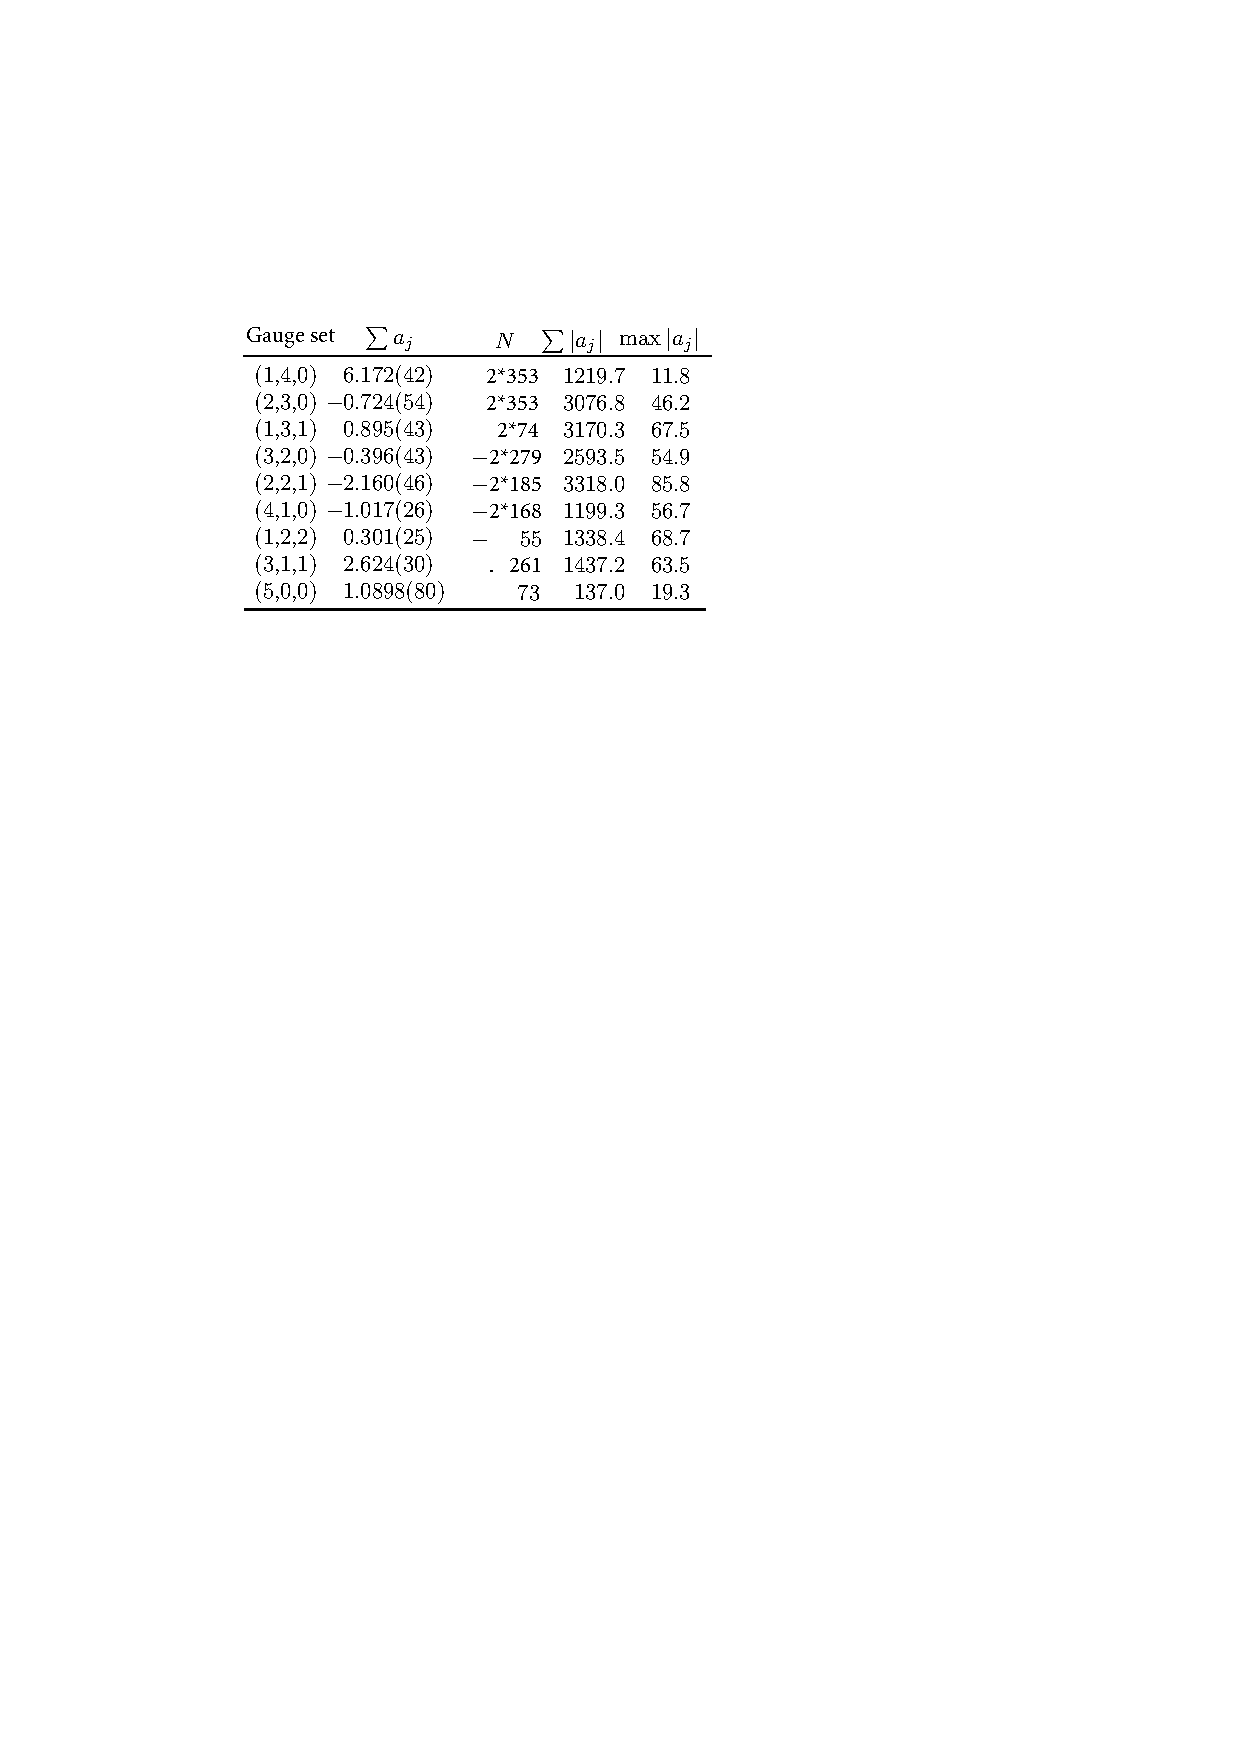
\includegraphics[width=0.60\textwidth]{Volkov19Tab1}
\end{center}
\caption{\label{Volkov19Tab1}
Contributions of the quenched QED $a^{(10)}[s]$ gauge sets, $s=(k,m,m')$.
If $m\neq m'$, the sum over $(k,m,m')+(k,m',m)$ is given, and the number
of contributing graphs is $2N_s$. Ignore the minus signs in $N$ column, a
PDF bug; I have also probably gotten the numbers of diagrams wrong.
Extracted from Volkov\rf{Volkov19} Table~1.
}
\end{table}
%%%%%%%%%%%%%%%%%%%%%%%%%%%%%%%%%%%%%%%%%%%%%%%%%%%%%%%%%%%

\item[2019-05-26 Predrag]
Volkov's
5-loop quenched QED gauge sets, are summarized in \reftab{Volkov19Tab1}.
Looking at the 4- and 5-loop results in \reftab{tabGaugeSets}, Volvkov surmises
that $(1,m,0)$ is approximately the final value, and the other values are
approximately zero with random errors (see {\bf 2018-12-21 Sergey} above).
However, gauge-set values surely do not look random to me; all signs except two
close to 0 follow my prediction, and the values are (unexplained) integers
multiples of 1/2.

Naive assumption would be that values of graphs contributing to gauge set
$s=(k,m,m')$ (do it separately from $s=(k,m',m)$ if $m\neq m'$) are uncorrelated
and randomly distributed, in which case one should test the randomness hypothesis by
computing the \emph{variance}
\beq
\expct{a^2_j}_{s} = \frac{1}{N_s}\sum_{j \in s} a^2_j
%\,.
\ee{variance_a_j}
for all gauge sets $s$ in \reftab{tabGaugeSets}, rather than listing $\sum
|a_j|$, as in Volkov's \reftab{Volkov19Tab1}, or my suggestion
\refeq{Volkov18AverMagn} above.
My interpretation of Volkov's $N_{diag}$ is likely wrong, as he writes that
``diagrams that are obtained from each other by changing arrow directions are
regarded as one,'' but that is easily fixed. It already seems that
$(5,0,0)$ and $(1,4,0)$ will be outliers.

More precisely, the {variance} is $\sigma^2=\expct{(a_j-\expct{a_j})^2}$,
and its positive square root is the \emph{standard deviation} $\sigma$.
This number depends on the gauge, and on particular auhtor's UV and IR
counter-term conventions, so it's hard to know what to make of it, but
getting a similar variance for all gauge sets would be cute.

\item[2019-06-04 Makiko Nio and Predrag to Sergey and Stefano] We have
looked together at the status of the 5-loop quenched QED, and what to do
to nail down the $4.5 \sigma$ difference between the two calculations.
Makiko's hunch is that the problem might be numerical, originating in a
Monte Carlo integral with a PDF defined in Seergey's \arXiv{1905.08007}
eq.~(1).

It looks to me that the ball is in Makiko's court; only way to compare is
via vertex diagram gauge sets, and she can do it if she really has to.

The first to check is $(5,0,0)$, both because it has the fewest diagrams,
and also because it is cleanest in terms of UV and IR counter terms. If
we ever manage to define and compute with a ``$k$-photon'' propagator,
$(k,0,0)$ has only one of them. Note also that max$|a_j|\approx 20$,
anomalously small.

$(1,4,0)$ (and the $(1,k,0)$ family of gauge sets) is fascinatingly
large. Our guess it that it might have to do with IR behaviour of the
4-loop self-energy insertion - Sergey can tell if there is something
going on there by looking at the contributing diagrams.
Note also that max$|a_j|\approx 10$, even more anomalously small, typical
size for the remaining gauge sets is max$|a_j|\approx 70$.

Next to knock off is $(1,2,2)$, then $(3,2,0)$. In my $1/2$ units I would
like to think of this set as well as $(2,2,0)$ as being approximately zero
(not to violate my gauge set sign rule).

\item[2019-09-19 Sergey] See Volkov\rf{Volkov19b} {\em }

\item[022-03-02 Sergey] See Volkov\rf{Volkov21}
{\em A way of fast calculating lepton magnetic moments in
Quantum Electrodynamics}

\item[2022-03-02 Sergey] See Volkov\rf{Volkov22}
{\em A flexible divergence elimination method for calculating
lepton magnetic moments in {Quantum Electrodynamics}}.
In principle I should check whether this is the same or different from
my methods...


\newpage
\item[2017-06-11 Predrag] to
\\
%Professor
Christian Schubert <schubert@ifm.umich.mx>
%\\
%Instituto de Física y Matem{\'a}ticas,\\
%Universidad Michoacana de San Nicol{\'a}s de Hidalgo,\\
%Ciudad Universitaria, C-3, Apdo. 2-82,\\
%C.P. 58040 Morelia, Michoacan, MEXICO
%
%\bigskip
%
%Dear Christian

Stefano Laporta  has recently published analytic values of all 4-loop
electron magnetic moment gauge sets, and they look very intriguing.
Sergey  A. Volkov has started evaluating individual 5-loop vertex
diagrams and is in position to estimate numerically the size of 5-loop
gauge sets. So it might be a good time to make a new attempt to prove/disprove
the QED finiteness conjecture. This set of notes is my current best attempt
to motivate this effort.

I do not take my 1977 ``gauge-set approximation'' very literally - its
content is only that if individual gauge sets can be bounded to anything
growing slower than combinatorially, quenched QED (and hopefully full
QED) is a finite theory, not an asymptotic series. But the form of vertex
gauge sets is very suggestive; it is defined in terms of $N$-photon
exchanges. So to me the wordline formalism seem the most promising way
forward.

While the quenched QED magnetic moment of electron is the cleanest
possible physical calculation one can do, for sociological reasons most
effort on high order estimates has gone in other directions. Do you have
a formula for spinor QED magnetic moment that one could attempt to
analyze more closely?

%As I have returned to this problem only last month, after a 40 year
%hiatus :) I would be grateful for any further pointers to the literature.

\item[2017-06-12 Christian]
I have been
fascinated by the finiteness conjecture ever after Gerald Dunne and I
were led there, too, from Euler-Heisenberg, Borel analysis,
Ritus mass shift and worldline instantons fifteen years ago.
The things have picked up a lot
just during the last year or so, namely:

\begin{enumerate}
  \item
Idrish Huet, Michel Rausch and I are working on the Affleck,
Alvarez and Manton (AAM) exponentiation conjecture\rf{AffAlMa82} in 1+1 QED.
We had a nice parameter integral representation for the three-loop
Euler-Heisenberg for quite a while, but could not get a sufficient number
of weak-field expansion coeffs out of it (so far what we got points to
AAM not holding at three loops - rather the coeffs go asymptotically
BELOW the AAM prediction - but this is very preliminary). Michel was just
visiting, and we now got a really nice algorithm (based on the polynomial
invariants of the dihedral group) for the analytical calculation of the
coeffs from the more difficult (nonplanar) 3-loop EH diagram.
  \item
If AAM really fails, then presumably the AAM worldline instanton needs
refinement at higher loops. My former student Naser Ahmadiniaz (now
postdoc in Korea) has made some progress with this.
  \item
For many years I am planning to apply the worldline formalism to (g-2),
in particular to the important graphs with the
light-by-light subdiagram. For this subdiagram I have, since a long time,
an off-shell representation that is permutation symmetric, manifestly
gauge invariant, without spurious UV poles, and moreover allows one to
trivially integrate out the one low-energy photon leg. What held me back
was that the various worldline representations that existed hitherto for
the electron line were all somewhat cumbersome, and seemed not suitable
for high-order calculations. Precisely this problem we have been working
on here for the last half year, and things have fallen into place really
nicely, we have a Bern-Kosower type master formula for the electron line
dressed with any number of photons, in vacuum and in the presence of a
constant field, and one of our students is already programming it. I am
now definitely trying to assemble a collaboration to attack the QED (g-2),
and I anticipate that your notes will be quite useful for motivating my
collaborators.

\end{enumerate}
Gies \etal\rf{GiSaVa05} have some intriguing numerical results from
worldline Monte Carlo (in section 5). Another thing I find quite
interesting are Ritus\rf{Ritus80} most recent
papers\rf{Ritus06,Ritus13,Ritus15} on the value of the bare fine
structure constant - he confirmed to me in an email from last December
(at age 90) that he definitely does not think that the bare charge is
infinite.

I am appending a summary of our efforts in this line of work\rf{HuTrSc17a}
which I wrote as a contribution to the 5th Winter Workshop on
Non-Perturbative Quantum Field Theory. 22-24 March 2017,
Sophia-Antipolis.

\item[2016-12-18 Vladimir I. Ritus] <v\_i\_ritus@mail.ru>
to Christian:

Thank you for your note about the papers by Johnson, Baker, Willey (Phys.
Rev. 1967, 1969, 1971) and by Adler, Bardeen (Phys. Rev. 1971).
    \PC{2017-08-04
    K. Johnson, M. Baker, and R. Willey, Phys. Rev. 136, B1111 (1964);
    ibid. 163, 1699 (1967); and
    S. L. Adler and W. A. Bardeen, Phys. Rev. D 4, 3045 (1971)
    These papers are about the possibility of the existence of an
    ultraviolet fixed point $\alpha_c$.
    }
I forgot them while writing my papers\rf{Ritus13,Ritus15}. Some months
ago I accidently saw  the abstracts of these papers in one of my
notebooks  with conspectus of the literature. Johnson et al assertion
confirms qualitatively my geometric and holographic duality approach to
the problem. Both of them deal with photons without self-energy
insertions. Have you any objections to this approach?

Nobody believes in infinite bare charge neither with space distribution
more singular than $\delta(x)$ nor as Landau pole at final transfer
momentum. Please, reed the several first phases in JRLR-paper (changing
the ``emitted"  to ``emitting").

I regret that I could not come to Tomsk, where I was at war time
1941-1943 in evacuation.

\item[2017-06-14 Christian to Ritus]
Just to make sure that I understand your conjecture correctly - are you
claiming that $1/4\pi$ is the value of the bare constant in the quenched
approximation, or in the full QED?

\item[2017-06-29 Vladimir Ritus]
The $1/4\pi$  is the value of the bare fine structure constant in the
full QED. It follows from duality of 4-dimensional QED and 2-dimensional
quantum field theory. The point charge moves  along timelike trajectory,
hence it has nonzero mass, but the photons emitted to infinity by this
charge are massless as the duality connected with them scalar quanta of
pairs emitted by the pointlike mirror in (1+1)-space. Constants
$\alpha_L$ and $\alpha_B$ are also geometrical. So, this theory is pure
geometrical and connected neither with the divergent perturbation theory
series, nor with the different methods of their summing. Please, read
\refrefs{Ritus13,Ritus15}.



\item[2017-06-18 Naser Ahmadiniaz] <ahmadiniaz.naser@gmail.com>
(currently a postdoctoral fellow at the Center for Relativistic Laser
Science (CoReLS), Institute for Basic Science (IBS), Gwangju, South
Korea).
\\
My main research
interests are in amplitude calculations in QED, QCD and quantum gravity
from the worldline formalism. Recently, we have been interested in
(off-shell) tree-level amplitudes for QED processes in vacuum as well as
in the presence of classical background fields which will also be applied
to higher order corrections.

\item[2017-06-20 James P. Edwards] <jedwards@ifm.umich.mx>,
%Instituto de Física y Matemáticas
%Universidad Michoacana de San Nicolás de Hidalgo
\HREF{www.ifm.umich.mx/ifm/index.php/fisca/academicos/edwards/}
{homepage}:
\\
I am currently working with Christian on the worldline approach. In some
of our recent work we have been working on more efficient ways to
determine g-2 based upon a worldline expression for the dressed spinor
propagator (both in vacuum and in a constant background).

\item[2017-06-11 Predrag] to
%\\
% Professor
Dirk Kreimer <kreimer@physik.hu-berlin.de>
%\\
%Humboldt-Universit\"at zu Berlin\\
%Institut f\"r Mathematik\\
%\bigskip
%
%Dear Dirk
%
%\medskip

Stefano Laporta  has recently published analytic values of all 4-loop
electron magnetic moment gauge sets, and they look very intriguing.
It might be a good time to make a new attempt to prove/disprove
the QED finiteness conjecture. This set of notes is my current best attempt
to motivate this effort.

If individual gauge sets can be bounded to anything growing slower than
combinatorially, quenched QED (and hopefully full QED) is a finite
theory, not an asymptotic series. The form of vertex gauge sets is
suggestive of a way forward; it is defined in terms of $N$-photon
exchanges. Hopf algebras might hold the key, but I do not know how to use
these ideas.

I would be grateful for any further pointers to the literature.
Anybody else I should send these notes to? And I'm
finally ready to stand up an be counted - I can fly to Berlin on a short
notice if that helps.

%\bigskip
%
%\noindent
%best regards
%\\
%Predrag
%\newpage

\item[2017-06-14 Dirk Kreimer] was kind enough to invite me to
\HREF{http://www2.mathematik.hu-berlin.de/~kreimer/wp-content/uploads/houches2018.html}
{Les Houches — June 4-15, 2018} on structures in local quantum field
theory. Edwards and I went, and learned a whole lot.

\item[2019-06-03 Christian Schubert and James P. Edwards]
We are still making sense of our master formulae but things are falling
into place. Our worldline efforts still are not paying off - a whole
class of terms that we had thought would not contribute on-shell for the
open fermion line actually does, And there is still the question whether
$g-2$ should be calculated in x-space or in p-space on the worldline
$\dots$ . We will keep you updated.

\item[2020-06-04 Somdatta Bhattacharya] <somdatta.bhattacharya@gmail.com>
writes: ``
I am intrigued by something you're an expert on. Soft photons correct the
QED vertex, so why don't they also affect $F_2(0)$ by a finite amount?
''
\\
{\bf Predrag} Dear Somdatta, \emph{you} are the expert\rf{Bhattacharya17}
:) Soft photons (were there an unambiguous gauge-invariant definition
that included both the IR divergences and the finite parts) contribute to
all radiative QED corrections, so surely they contribute to $g-2$
anomaly.

Here is my 5 cents. It's hand-waving, so I only say it in the privacy
of my QFT class - if you can turn it into mathematics, I would be grateful.

For me the IR and UV divergences exist on the same footing, even
cancelling each other\rf{MassShell}. However, the anomaly
\refeq{IRstruct(1)Q} does not have either\rf{IRstruct}. Why?

$F_2(0)$ part of the QED vertex form factor corresponds to flipping
the electron spin; soft photon cannot do that, that's why there is no
IR divergence. When you look at the parametric form of the
integral for $a_{0}^{(2)}$ it looks like the dominant contribution
is halfway where the infrared and ultraviolet singularities
would have been. So in my book, the soft photons are about 50\%
of the $F_2(0)$ anomaly.

PS If you actually read {\em Infra-red structure of {Yang-Mills}
theories}\rf{IRstruct}, it is not a stupid paper. That's why is has
garnered the total of 14 citations. I would be grateful for any earlier
(or later) reference that does it better or explains it more clearly.

PPS Maybe I should read
Fleischer and Tarasov\rf{FleTar92}
{\em Gauge-invariant on-shell {$Z_1$} in {QED} and {QCD}}?
(I do not have access to it online)

\item[2020-06-04 Somdatta Bhattacharya]
Here's my argument for why the $F_2(0)$ is zero at least up to first order,
but I end with a conundrum.

The amplitude for the vertex with the soft photon is akin to the Compton
scattering amplitude, with one of the photons being the soft one and the
other being the one of the vertex. In the limit of small photon momenta,
it is proportional to
$\overline{u}(p'.e/p'.k - p.e/p.k)\gamma^mu$
sandwiched
between the electron spinor states, where p' and p are the electron
momenta and k is the soft-photon one, e being the soft photon
polarization.

In the usual analysis, when you sum over polarizations and integrate for
the invariant momentum measure for k over the square of the expression
you get the Sudakov double logs in the scattering amplitude, that cancel
a similar expression coming from the loops, that is the $F_1$. I am
following Peskin and Schroeder.

Notice that the expression for the soft photons is exact, so that is all
that is there to it, and hence it doesn't give any contribution to
$F_2(0)$.

However, here's something interesting.

You get $(p'.e/p'.k-p.e/p.k)$ by acting with the Dirac operators on
specific spinors on either side of the Compton amplitude. But what if you
exchange p' and p by using momentum conservation and make the
corresponding Dirac operators act on the spinors on opposite sides. You
would get a totally different expression, involving
$[(p'.)/p'.k-(p.)/p.k](\gamma.e)$.
Now, ``in principle" such an expression ought to be
re-expressible in terms of
\(
\sigma. q.e. (F_2(p,p',k)) + \gamma.e(F_1(p,p',k))
\)
for some $F_2$ and $F_1$. The dots in the subscripts stand for greek
indices in the sigma expression.

And when squared and integrated over would give rise to a Rosenbluth-like
formula for electron scattering when one does the integral over k, from
which one can extract the ``effective" F's. Then setting the q to zero,
one should get the $F_2(0)$. Notice that like the $F_1$, this too would be
possibly divergent.

The only trouble is the finite q expressions should match with the result
computed using $(p'.e/p'.k - p.e/p.k)$, which gives just an $F_1$. But
this can't be possible, but I can't figure out the mistake in the naive
analysis. This is the conundrum I was referring to.

This is all I have come up with till now.

Here's something you might find of interest: \\
\emph{alternative worldline new.pdf} ;\;
\emph{SM from GR.pdf} \,.

Here's a rough draft I have written on new ways of doing QED one-loop calculations and their advantages. It's meant to open up discussions/collaboration:
\emph{QED new.pdf}.
Please take a look and let me know what you feel.

\item[2022-12-30 Christian Schubert]
Vladimir Ritus seems to be very anxious to have your opinion on
his papers about the calculation of alpha.

\item[2023-04-10 Sergey] sergey.volkov.1811@gmail.com \\
    Did you try to extend gauge-invariant classes beyond QED towards EW? For
    example, to take into account the difference between left and right
    electrons?
\item[2023-04-10 Predrag]
No, I did not.

The only new thing I have been thinking about is whether there is a
gauge-invariant planar field theory (the papers are
\HREF{ChaosBook.org/~predrag/papers/preprints.html\#PlanFieldThe} {here}) version of
QED. That would give a new, perturbatively convergent approximation to
QED. Lauwers, Scharbach and I had worked it out for QCD, in particular the
Ward identities  (7.17), but I do not remember why we did not apply it to
QED, which should be a simpler, special case.

I do not know if you know, but Kinoshita died recently. A very remarkable
man. I'll try to rework the notes I sent to you a long time ago as a paper in
his memory.


\end{description}

    % reducesymm/QFT/finiteBlog.tex  compile by  pdflatex blog; bibtex blog
% $Author$ $Date$
% Predrag  switched to github.com               jul  8 2013

\section{QCD gauge sets - a blog}
\label{sect:QCDgaugeSets}

In 1981 Cvitanovi\'c \etal\rf{NPB81} constructed gauge invariant
subsectors in QCD.


\begin{description}

\item[2016-12-10 Predrag]
Penante\rf{Penante16} 2016 {{On-shell methods for off-shell quantities in N=4
Super Yang-Mills: from scattering amplitudes to form factors and the
dilatation operator}} has an up-to-date review of on-shell methods.

\item[2016-12-26 Predrag] Read
Cruz-Santiago, Kotko and Sta{\'s}to\rf{CrKoSt15} 2015
{\em Scattering amplitudes in the light-front formalism}:
``The idea is to divide the process into appropriate gauge invariant
components. It turns out that the gauge invariant subsets are invariant
under cyclic permutations of the external gluons. This decomposition was
proposed in works of [58–61] for the tree level amplitudes. A thorough
analysis of the relation between color structures and gauge invariance
was done in \refref{NPB81}. The color decomposition principle was
extended beyond the tree level to loop amplitudes in [63].''

\item[2016-12-26 Predrag]
Should also read Dixon\rf{Dixon96} 1996
{\em Calculating scattering amplitudes efficiently}.



\item[2017-05-26 Predrag]
The decomposition of scattering amplitudes into gauge invariant subsets
of diagrams is studied by Boos and Ohl\rf{BBLOM94,BooOhl99}.
Boos and Ohl\rf{BooOhl99}
{\em Minimal gauge invariant classes of tree diagrams in gauge theories},
\arXiv{hep-ph/9903357} (see \arXiv{hep-ph/9911437} and
\arXiv{hep-ph/0307057} for more detail) is motivated by applications to
Standard Model multi-particle diagrams, mostly at the tree level.

Perturbative calculations require an explicit breaking of gauge
invariance for technical reasons and the cancellation of unphysical
contributions is not manifest in intermediate stages of calculations. The
contribution of a particular Feynman diagram to a scattering amplitude
depends in the gauge fixing procedure and has no physical meaning.
the identification of partial sums of Feynman diagrams that are gauge
invariant by themselves is of great practical importance.
Calculation a subset of diagrams that is not gauge invariant has no
predictive power, because they depend on unphysical parameters introduced
during the gauge fixing.

A \emph{gauge invariance class} is a minimal subset of Feynman diagrams
that is independent of the gauge parameter and satisfies the
Slavnov-Taylor identities.

The set of diagrams connected by flavor and gauge flips they call
\emph{forest}, a set of diagrams connected by gauge flips the call
\emph{grove}. They shown that the groves are the minimal gauge invariance
classes of tree Feynman diagrams. In unbroken gauge theories, the
permutation symmetry of external gauge quantum numbers can be used to
subdivide the scattering amplitude corresponding to a grove further into
gauge invariant sub-amplitudes.

This (largely uncited) work seems to have no impact on the $(g-2)$
gauge sets discussed here.

\item[2017-05-27 Predrag]
Reuschle and Weinzierl\rf{ReuWei13} {\em Decomposition of one-loop {QCD}
amplitudes into primitive amplitudes based on shuffle relations}
cite our \refref{NPB81}. They say:

QCD calculations organise the computation of the one-loop amplitude as a sum
over smaller pieces, called \emph{primitive amplitudes}.
The most important features of a primitive amplitude are gauge invariance
and a fixed cyclic ordering of the external legs.
Primitive amplitudes should not be confused with \emph{partial amplitudes}
(also referred to as a \emph{dual amplitude} or a \emph{color-ordered amplitude}),
which are the kinematic coefficients of the independent colour
structures.
The first step in a discussion of perturbative Yang-Mills is the
decoupling of color from kinematics,
\beq
A_{tot} = \sum c_J A_J
\ee{KolShi14(1.1)}
where $A_{tot}$ represents the total amplitude for a scattering process,
$A_J $ are all the possible color structures,
and $A_J$ are partial amplitudes which depend only on the kinematical data
(momenta and polarizations).
Partial amplitudes are gauge invariant, but not
necessarily cyclic ordered.
Partial amplitudes are far simpler to calculate than the
full amplitude. There
exist linear relations among the partial amplitudes, called
Kleiss-Kuijf relations, which reduce the number of linearly
independent partial amplitudes to $(n-2)!$
The leading contributions in an $1/N$-expansion (with $N$ being the number of colours)
are usually cyclic ordered, the sub-leading parts are in general not.
The decomposition of the full one-loop amplitude into partial amplitudes is easily derived.
However, it is less trivial to find a decomposition of the partial
amplitudes into primitive amplitudes.

There are several possible choices for a basis in colour space.
A convenient choice is the colour-flow basis\rf{tHooft:1974jz}.

\item[2017-05-27 Predrag]
Schuster\rf{Schuster14} {\em Color ordering in {QCD}}: ``
We derive color decompositions of arbitrary tree and one-loop QCD
amplitudes into color-ordered objects called primitive amplitudes.
''

\item[2017-05-27 Predrag]
Zeppenfeld\rf{Zeppenfeld88}
{\em Diagonalization of color factors} (Georgia Tech has no access to this paper)

\item[2017-05-27 Predrag]
Edison and Naculich\rf{EdiNac12} {\em Symmetric-group decomposition
of {SU(N)} group-theory constraints on four-, five-, and six-point
color-ordered amplitudes at all loop orders}: ``
Color-ordered amplitudes for the scattering of n particles in the adjoint
representation of SU(N) gauge theory satisfy constraints that arise from
group theory alone. These constraints break into subsets associated with
irreducible representations of the symmetric group $S_n$, which allows
them to be presented in a compact and natural way.
''

\item[2017-05-27 Predrag]
Kol and Shir\rf{KolShi14,KolShi15}
{\em Color structures and permutations} has a
useful overview of the literature in the introduction, and is a very
interesting read overall.

We may permute (or re-label) the external legs in the expression for a
color structure and thereby obtain another color structure. This means
that the space of color structures is a representation of $S_n$, the
group of permutations. A natural question is to characterize this
representation including its character and its decomposition into
irreducible representations (irreps).

The decomposition of color structures into irreps was suggested by
Zeppenfeld\rf{Zeppenfeld88}.

The space of tree-level color structures $TCS_n$ of dimension
\beq
\mbox{dim}(TCS_n) = (n-2)!
\ee{KolShi14(2.7)}
is the vector space
generated by all diagrams with $n$ external legs and an oriented cubic
vertex, which are connected and without loops (trees), where diagrams
which differ by the Jacobi identity are to be identified.

The $f$-based and $t$-based color structures are related by celebrated
Kleiss-Kuijf\rf{KleKui89} relations (rederived in this paper).

The original problem, that of capturing symmetries of the partial
amplitudes which originate with those of the color structures, is now
formulated as the problem of obtaining the $S_n$ character
of the space of color structures. It turns out that (at least at
tree level) this problem was fully solved in the mathematics literature
by Getzler and M. M. Kapranov\rf{GetKap98}.

The free Lie algebra over some set $A$, denoted by $L(A)$, is the Lie
algebra generated by $A$ with no further relations apart for antisymmetry
and the Jacobi identity which are mandated by definition.

Self duality under Young conjugation: for some $n$ values $TCS_n$  is
self-dual under Young conjugation, namely under the interchange of rows
and columns in the Young diagrams

\item[2017-05-27 Predrag]
Getzler and Kapranov\rf{GetKap98} {\em Modular operads}: ``
We develop a `higher genus' analogue of operads, which we call modular
operads, in which graphs replace trees in the definition. We study a
functor $F$ on the category of modular operads, the Feynman transform,
which generalizes Kontsevich's graph complexes and also the bar
construction for operads. We calculate the Euler characteristic of the
Feynman transform, using the theory of symmetric functions: our formula
is modelled on Wick's theorem.
''

\item[2017-05-27 Predrag]
Maltoni \etal\rf{MPSW03}
{\em Color-flow decomposition of {QCD} amplitudes}

The \emph{color-flow} decomposition is based on treating the $SU(N)$
gluon field as an $N\!\times\!N$ matrix.
(PC: I think that is what I actually do.)
It has several nice features.
First, a similar decomposition exists for all multiparton amplitudes,
like the fundamental-representation decomposition. Second, the color-flow
decomposition allows for a very efficient calculation of multiparton
amplitudes. Third, it is a very natural way to decompose a QCD amplitude.
As the name suggests, it is based on the flow of color, so the
decomposition has a simple physical interpretation.

To calculate the amplitude, one orders the gluons clockwise, and draws
color-flow lines, with color flowing counterclockwise, connecting
adjacent gluons. One then deforms the color-flow lines in all possible
ways to form the Feynman diagrams that contribute to this partial
amplitude. The Feynman diagrams that contribute to a partial amplitude
are planar. This is not due to an expansion in $1/N$; the partial
amplitudes are exact. They note (see their Table 1) that the number of
Feynman diagrams contributing to an $n$-gluon partial amplitude grows as
$\approx 3 \cdot 8^n$. In contrast, the number of Feynman diagrams
contributing to the full amplitude grows factorially, as
$\approx (2n)!$.


%\item[2017-05-27 Predrag] in the spirit of Feynman's challenge,
%track the progeny o gauge sets
%
%(1,0,0) $\to$ (2,0,0) + ((1,1,0) + (1,0,1))
%
%(2,0,0) $\to$ (3,0,0) + ((2,1,0) + (2,0,1))
%
%((1,1,0) + (1,0,1)) $\to$ (1,1,1) + ((2,0,1) +  + (1,0,2))
%
%
%(1,1,0),
%
%(2,0,0)
%
%(1,0,1)

\item[2017-06-09 Predrag]
Henn \etal\rf{HLSSS17}
{\em Four-loop photon quark form factor and cusp anomalous dimension in
the large-{$N_c$} limit of {QCD}}, \arXiv{1612.04389}, is a thoroughly
modern paper, a listing of different codes used to generate diagrams and
evaluate integrals.

\item[2017-06-16 Predrag]
Chang, Liu and Roberts\rf{ChLiRo11}
{\em Dressed-quark anomalous magnetic moments}

\item[2017-06-16 Predrag]
Choudhury and Lahiri\rf{ChoLah15}
{\em Anomalous chromomagnetic moment of quarks}

\item[2017-06-16 Predrag]
Bermudez \etal\rf{BAGTB17}
{\em Quark-gluon vertex: {A} perturbation theory primer and beyond},
\arXiv{1702.04437}:
The on-shell limit enables us to compute anomalous chromomagnetic moment
of quarks.

[...] we present some ``physically" relevant results for
the on-shell limit $p^2=k^2=m^2$ and $q^2=0$. The Dirac and Pauli
form factors, $F_1(q^2)$ and $F_2(q^2)$, respectively, define the
Gordon decomposition of the quark current as in \refeq{BAGTB17(35-1)}.
The anomalous chromomagnetic moment (ACM) of quarks can be
identified as $F_2(q^2)$ for $q^2 \rightarrow 0$. The Abelian
version of this decomposition with $C_F=1$ and $C_A=0$ is the
electron-photon vertex of quantum electrodynamics. The great
successes of the Dirac equation is the prediction of the magnetic
moment of a charged fermion  ${ {\mu}} = {eg}/{(2 m)} { S}$.
The radiative corrections lead to\rf{Schwinger48}
 \bea
 \frac{e}{2 m} \Rightarrow \left( 1 + \frac{\alpha}{2 \pi} \right) \frac{e}{2
 m}.
 \eea
Note that the quark-gluon vertex differs from the electron-photon vertex
already at one loop, by the contributions of an additional Feynman
diagram, involving the triple-gluon vertex. In fact, apart from
introducing additional color structure, this non-Abelian diagram
introduces, at the one-loop level, a kinematical structure which is
absent in the QED.

It is straightforward to see that for the soft gluon limit, $q^2=0$, the
Abelian contribution for the ACM reduces to the non-Abelian counterpart
of Schwinger's result, $F_{2}^{a}(0) = - \alpha /12 \pi$, already derived
in \refref{ChLiRo11}. On the other hand, the corresponding non-Abelian
contribution yields a divergence\rf{ChoLah15}, for a non-zero quark mass,
$m \neq 0$. We find this divergence to be logarithmic. For deep infrared
gluon momenta it behaves as $F_2^{b}(q^2 \rightarrow 0)= C_b \ln \left( -
q^2/m^2 \right)$. Of course, perturbation theory in QCD is not the way to
explore deep infrared region. All perturbative conclusions will be taken
over by non-perturbative effects, overshadowing this divergence.

\item[2017-06-16 Predrag]
Brambilla \etal\rf{Brambilla14}
{\em {QCD} and strongly coupled gauge theories: challenges and perspectives}

\item[2017-06-16 Predrag]
Simonov and Tjon\rf{SimTjo02}
{\em The {Feynman–Schwinger} representation in {QCD}}:``
The proper time path integral representation is derived for Green's
functions in QCD. After an introductory analysis of perturbative
properties, the total gluonic field is separated into a nonperturbative
background and valence gluon part. For nonperturbative contributions the
background perturbation theory is used systematically, yielding two types
of expansions. As an application, we discuss the collinear singularities
in the Feynman–Schwinger representation formalism.
''



\end{description}

\newpage
\section{Is QED finite? A blog}
\label{sect:finiteBlog}

\begin{description}

\item[1950-12-22 Schwinger]
{\em On gauge invariance and vacuum polarization}\rf{Schwinger51c}
has 3700 citations.
He writes: ``
This paper is based on the elementary remark that the extraction of gauge
invariant results from a formally gauge invariant theory is ensured if
one employs methods of solution that involve only gauge covariant
quantities. We illustrate this statement in connection with the problem
of vacuum polarization by a prescribed electromagnetic field. The vacuum
current of a charged Dirac field, which can be expressed in terms of the
Green's function of that field, implies an addition to the action
integral of the electromagnetic field. Now these quantities can be
related to the dynamical properties of a ``particle" with space-time
coordinates that depend upon a proper-time parameter. The proper-time
equations of motion involve only electromagnetic field strengths, and
provide a suitable gauge invariant basis for treating problems. Rigorous
solutions of the equations of motion can be obtained for a constant
field, and for a plane wave field. A renormalization of field strength
and charge, applied to the modified lagrange function for constant
fields, yields a finite, gauge invariant result which implies nonlinear
properties for the electromagnetic field in the vacuum.
[...]
one can employ an expansion in powers of the potential vector. The latter
automatically yields gauge invariant results, provided only that the
proper-time integration is reserved to the last. This indicates that the
significant aspect of the proper-time method is its isolation of
divergences in integrals with respect to the proper-time parameter, which
is independent of the coordinate system and of the gauge. The connection
between the proper-time method and the technique of ``invariant
regularization" is discussed. Incidentally, the probability of actual
pair creation is obtained from the imaginary part of the electromagnetic
field action integral. Finally, as an application of the Green's function
for a constant field, we construct the mass operator of an electron in a
weak, homogeneous external field, and derive the additional spin magnetic
moment of $\alpha/2\pi$ magnetons by means of a perturbation calculation
in which proper-mass plays the customary role of energy.
''

``
A proper time wave equation, in conjunction with the second order
Dirac operator, has been discussed by
V. A. Fock\rf{Fock37}
{\em Proper time in classical and quantum mechanics}.
See also Nambu\rf{Nambu50} (1950).
''

In Appendix~B Schwinger computes the anomalous spin magnetic
moment $\alpha/2\pi$ produced by second-order electromagnetic mass effects.

\item[1977-03-03 Drell and Pagels]
{\em Anomalous magnetic moment of the electron, muon, and nucleon}\rf{DrePag65}
attempt got the sign right, but was not successful in predicting the
magnitude of the sixth-order magnetic moment;
$0.15 \left(\frac{\alpha}{\pi}\right)^3$ instead of
$1.19 \left(\frac{\alpha}{\pi}\right)^3$.

\item[1971-08-01 Lautrup, Peterman, and de Rafael]
 1972 {\em Recent
developments in the comparison between theory and experiments in quantum
electrodynamics}\rf{LaPeRa72} list the 3-loop, no-electron loop ``gauge invariant
subclasses'' (their Fig.~4.3).

\item[1974-01-07 Samuel]
1974 {\em Estimates of the eighth-order corrections
to the anomalous magnetic moment of the muon}\rf{Samuel74}:

``We speculate that in making radiative corrections to a class of graphs
by inserting a single photon in all possible ways, one obtains a
contribution which is roughly $-\frac{\alpha}{\pi}$ times the
contribution of the class. This seems to be obeyed by the known
contributions.''

\item[2013-11-24  Predrag]
As far as I can tell, terminology ``of \emph{quenched} type'' was first
introduced in this context by
Marinari, Parisi and Rebbi\rf{MaPaRe81}
{\em {Monte Carlo} simulation of the massive {Schwinger} model},
in the context of lattice gauge theory. They write:
``A first approximation to the effect of the gauge field on the fermion
observables may be achieved by [...] neglecting the contributions from
the fermionic vacuum polarization diagrams and, using a terminology
developed in the theory of condensed matter, we shall call the
expectation values thus obtained `quenched'",

Parisi is reputable, so in the ``quenched approximation" one neglects
the fermionic vacuum polarization effects (i.e, the fermion loops) from
the fermion determinant in the effective action. If it is good enough for Kinoshita,
it is good enough for you.

``In the ‘quenched approximation’ the quark determinant is set equal to
unity, i.e., neglecting the effect of virtual quark loops. In
other words, this extreme approximation in terms of heavy quarks with a
vanishing number of flavors assumes that gauge fields affect quarks while
quarks have no dynamical effect on gauge fields."

A more general usage: ``In Quantum Cosmology ‘‘quenching,’’ amounts to
quantizing a single scale factor thereby selecting a class of
cosmological models, for instance, the Friedmann-Robertson-Walker
space-time while neglecting the quantum fluctuations of the full
metric.''

But I still do not like it - it is mostly associated with Kogut, where it
means something different (as in ``... treating the gauge interaction in
the quenched, planar (ladder) approximation"); search for quench
\HREF{http://en.wikipedia.org/wiki/Quantum_chromodynamics} {here}. Or
here is what Brezin says:

``concept of quenching is well-known in the statistical mechanics of
random media ; consider a system of particles, for instance, an electron
gas, interacting with impurities. If these impurities are mobile, they
will thermalize with the electron gas and the average physical quantities
are obtained by a trace over the electron gas and the impurities degrees
of freedom. However if the impurities are frozen, the `quenched' case,
the physical observables are obtained by calculating their value for
fixed impurities and then averaging over these
impurities. "

That is how I know it - nothing about fermion loops, just dirt physics...

From my point of view, the question is whether the sum of all
corrections to (g-2) is a convergent series, or an asymptotic one.
If on can prove the convergence for the quenched sector, I would
expect each un-quenched sector (diagrams with one, two, .... lops)
separately to be convergent, and their sum as well.

Here is something to amuse you:
\HREF{http://www.scottaaronson.com/blog/?p=1537}{on amplituhedron}.
More serious: Lance Dixon
\HREF{http://www.preposterousuniverse.com/blog/2013/10/03/guest-post-lance-dixon-on-calculating-amplitudes/}
{on calculating amplitudes}.

The inventor of the ``gauge invariant diagram sets" concept is Benny
Lautrup.

\item[2013-12-08  Predrag] to Piotr, Wanda and Andrea
(Piotr Czerski <piotr.czerski@ifj.edu.pl>,
 wanda.alberico@to.infn.it,
 andrea.prunotto@gmail.com):

I'm no fan of Feynman diagrams (my rant is
\HREF{http://www.cns.gatech.edu/~predrag/papers/preprints.html\#FiniteFieldTheo}
{here}), and I'm always looking
for other ways to look at perturbative expansions. So just a little email
- if you have a new angle\rf{PrAlCz13} on subsets of diagrams which are gauge
invariant sets, I would be curious to learn how you look at that.

Just something to keep in mind :)

PS to Andrea: I realize you might rather forget this stuff (takes you a
decade to write a paper?) but at least I got a ringtone out of you. The
only problem is, I do not have a cell phone, so I do not know how to make
it ring. At least I'm more technologically savvy than
\HREF{http://www.theguardian.com/science/2013/dec/06/peter-higgs-boson-academic-system?CMP=twt_gu}
{Peter Higgs}.

\item[2013-12-10  \HREF{https://sites.google.com/site/andreaprunotto/} {Andrea}]
Sorry for late reply (well, we're used to longer gaps). Yes! I actually
took 10 years to write this paper out of my master thesis, but I have
some excuses: I did my PhD in Biochemistry (Z\"urich) and now I work on
genetics (Lausanne). This summer my ``old'' professor Wanda found my work
in a drawer and then contacted me, telling me that it would be a good
idea to publish it.

About your request: I'm really interested in seeing if the rooted-map
approach to Feynman diagrams can address the problem you've risen. But I
have no idea what the ''subsets of diagrams which are gauge invariant
sets'' are. I've checked a bit on the web but I'm sure you can give me
better indications (the works I found were too technical: I need to know
the basis of the problem). Can you send me some specific link at freshman
level, in particular where I can see the geometry of these subclasses of
diagrams?

\item[2013-12-11  Predrag]
Googling is good, but it is faster to click on
\HREF{http://www.cns.gatech.edu/~predrag/papers/preprints.html\#FiniteFieldTheo}
{this link}. The article defines the gauge invariant sets.

\item[2014-02-11 M. Borinsky]
\emph{Feynman graph generation and calculations in the Hopf algebra of
Feynman graphs}\rf{Borinsky14}
``Programs for the computation of perturbative expansions of quantum
field theory amplitudes are provided. feyngen can be used to generate
Feynman graphs for Yang-Mills, QED and $phi^k$ theories. feyncop
implements the Hopf algebra of those Feynman graphs which incorporates
the renormalization procedure necessary to calculate finite results in
perturbation theory of the underlying quantum field theory. ''

\item[2016-02-08  Predrag]
Prunotto\rf{Prunotto03}
{\em A Homological Approach to Feynman Diagrams in the Quantum Many-Body Theory},
and
Prunotto, Alberico and Czerski\rf{PrAlCz13} 2013
{\em Feynman Diagrams and Rooted Maps}
has been submitted to the European Physical Journal A as manuscript ID EPJA-103480,
seems not to have been published anywhere by 2017.
%I have been asked to referee it, but have declined - too busy.
They write: ``
The  Rooted Maps Theory, a branch of the Theory of Homology, is shown to be
a powerful tool for investigating  the topological properties of Feynman
diagrams, related to the single particle propagator in the quantum many-body
systems. The numerical correspondence between the number of this class of
Feynman diagrams as a function of perturbative order and the number of rooted
maps as a function of the number of edges is studied. A graphical procedure to
associate Feynman diagrams and rooted maps is then stated. Finally, starting
from rooted maps principles, an original definition of the genus of a
Feynman diagram, which totally differs from the usual one, is given.
''

\item[2017-03-15 Predrag]
Dunne and Krasnansky\rf{DunKra06} 2006 {\em ``Background field
integration-by-parts'' and the connection between one-loop and two-loop
{Heisenberg-Euler} effective actions}: ``
We develop integration-by-parts rules for diagrams involving massive
scalar propagators in a constant background electromagnetic field, and
use these to show that there is a simple diagrammatic interpretation of
mass renormalization in the two-loop scalar QED Heisenberg-Euler
effective action for a general constant background field. This explains
why the square of a one-loop term appears in the renormalized two-loop
Heisenberg-Euler effective action, and
dramatically simplifies the computation of the renormalized two-loop
effective action for scalar QED, and generalizes a previous result
obtained for self-dual background fields.
''

\item[2017-05-23 Predrag]
\phantomsection \label{sect:SchSch96}
M. G. Schmidt and C. Schubert\rf{SchSch96} 1994
{\em Multiloop calculations in the string-inspired formalism: the single
spinor-loop in QED}, \arXiv{hep-th/9410100}:
They use the worldline path-integral Bern-Kosower formalism
for to calculate the sum of all diagrams
with one spinor loop and fixed numbers of external and internal photons.
Of interest: in this formalism the three 2-loop photon polarization graphs,
see \reffig{BHSTW143loopphotonprop},
are a single integral, easier to evaluate than any of the three Feynman
graphs. They also note an unexplained cancelation not only of poles, but also
of ``transcedentals.''
A knot-theoretic explanation for the rationality of the quenched
QED beta function is given in \refref{BrDeKr96}.

\item[2017-05-23 Predrag]
Nieuwenhuis and Tjon\rf{NieTjo96} 1996
{\em Nonperturbative study of generalized ladder graphs in a {$\phi^2\chi$} theory},
\arXiv{hep-ph/9606403}:

\item[2017-05-23 Predrag]
Christian Schubert\rf{Schubert01} 2001
{\em Perturbative quantum field theory in the string-inspired formalism},
\arXiv{hep-th/0101036}:

The Feynman rules for (Euclidean) spinor QED in the second order
formalism (see Morgan\rf{Morgan95} 1995,
Strassler\rf{Strassler92} 1992, and references therein) are, up to
statistics and degrees of freedom, the ones for scalar QED with the
addition of a third vertex. % (Fig. 17).
The third vertex involves
$\sigma^{\mu\nu}={1\over 2}[\gamma^{\mu},\gamma^{\nu}]$
and corresponds to the $\psi^{\mu}F_{\mu\nu}\psi^{\nu}$
-- term in the worldline Lagrangian $L_{\rm spin}$.
%(compare eq.(\ref{Weucl})).
For the details and for the non-abelian case see Morgan\rf{Morgan95}.
There also an algorithm is given, based on the Gordon identity, which
transforms the sum of Feynman (momentum) integrals resulting from the
first order rules into the ones generated by the second order rules.

\item[2017-06-12 Predrag]
Morgan\rf{Morgan95}
{\em Second order fermions in gauge theories}, \arXiv{hep-ph/9502230}
seems to be the same discussion that I use in my QFT course to define the
electron magnetic moment via $\sigma^{\mu\nu}$ (see lectures 25 and 26
\HREF{http://chaosbook.org/~predrag/courses/PHYS-7147-13/schedule.xml}
{here})

\item[2017-06-12 Predrag]
Gies, Sanchez-Guillen, V{\'a}zquez\rf{GiSaVa05}
{\em Quantum effective actions from nonperturbative worldline dynamics},
 \arXiv{hep-th/0505275}: ``
We demonstrate the feasibility of a nonperturbative analysis of quantum
field theory in the worldline formalism with the help of an efficient
numerical algorithm. In particular, we compute the effective action for a
super-renormalizable field theory with cubic scalar interaction in four
dimensions in quenched approximation (small- N f expansion) to all orders
in the coupling. We observe that nonperturbative effects exert a strong
influence on the infrared behavior, rendering the massless limit well
defined in contrast to the perturbative expectation.
''

\item[2017-06-12 Predrag]
Giesand H{\"a}mmerling\rf{GieHam05}
{\em Geometry of spin-field coupling on the worldline},
\arXiv{hep-th/0505072}:

\item[2017-03-15 Predrag]
Huet, McKeon, and Schubert\rf{HuMcSc10} 2010
{\em {Euler-Heisenberg} lagrangians and asymptotic analysis in 1+1 {QED. Part I: Two}-loop}
(no GaTech online access, \arXiv{1010.5315}):``
We continue an effort to obtain information on the QED perturbation
series at high loop orders, and particularly on the issue of large
cancellations inside gauge invariant classes of graphs, using the example
of the l-loop N-photon amplitudes in the limit of large photon
numbers and low photon energies. The high-order
information on these amplitudes can be obtained from a nonperturbative
formula, due to Affleck \etal\rf{AffAlMa82}, for the imaginary part of the QED
effective lagrangian in a constant field. The procedure uses Borel
analysis and leads, under some plausible assumptions, to a number of
nontrivial predictions already at the three-loop level. Their direct
verification would require a calculation of this `Euler-Heisenberg
lagrangian' at three-loops, which seems presently out of reach
(though see Huet, de Traubenberg, and Schubert\rf{HuTrSc17} below). Motivated
by previous work by Dunne and Krasnansky\rf{DunKra06} on Euler-Heisenberg
Lagrangians in various dimensions, in the present work we initiate a new
line of attack on this problem by deriving and proving the analogous
predictions in the simpler setting of 1+1 dimensional QED. In the first
part of this series, we obtain a generalization of the formula of
Affleck \etal\rf{AffAlMa82}
to this case, and show that, for both scalar and spinor QED, it
correctly predicts the leading asymptotic behaviour of the weak field
expansion coefficients of the two loop Euler-Heisenberg lagrangians.

``The present work continues an
effort\rf{DunSch02I,DunSch02II,MaScVi03,DunSch06} to study the multiloop
behaviour of the QED $N$-photon amplitudes using the QED effective
lagrangian, and in particular to prove or disprove Cvitanovi\'c's
conjecture for these amplitudes.''

\item[2017-05-24 Predrag]
Bastianelli, Huet, Schubert, Thakur and Weber\rf{BHSTW14} 2014
{\em Integral representations combining ladders and crossed-ladders}
write:

This property is particularly interesting in view of the fact that it is
just this type of summation which in QED often leads to extensive
cancellations, and to final results which are substantially simpler than
intermediate ones (see, e.g., \refref{Cvit77b,BrDeKr96}). More recently, similar
cancellations have been found also for graviton amplitudes (see, e.g.,
\refref{BaBjVa09}).
Although this property of the worldline formalism is well-known, and has
been occasionally exploited\rf{rossch96a,rossch96b, SchSch96,BaRoSt06} (see also
\refref{FriGab12}) a systematic study of its implications is
presently still lacking.

The first classes of Green's functions %, depicted in fig. \ref{fig:Nprop},
is the
$x$-space propagator for one scalar interacting with the second one
through the exchange of $N$ given momenta.

This object, to be called ``$N$-propagator'', is given by a set of $N!$
simple tree-level graphs, is in the worldline formalism combined into a
single integral.

The second class are the similarly looking  $x$-space $N+2$ - point
functions %shown in fig \ref{fig:halfladder},
defined by a line connecting
the points $x$ and $y$ and $N$ further points $z_1,\ldots,z_N$ connecting
to this line in an arbitrary order.

An advantage of the worldline representation over the usual Feynman
parameterization is the automatic inclusion of all possible ways of
crossing the ``rungs'' of the ladders. They obtain such representations
in explicit form both in $x$-space and in momentum space.

The inclusion of the crossed ladder graphs is essential for the
consistency of the one-body limit where one of the constituents becomes
infinitely heavy, and for maintaining gauge invariance.

They concentrate on the case of infinite $N$, \hbox{\it i.e.}, the sum
over {\it all} ladder {\it and} crossed ladder graphs.

As their main application, they consider the case of two massive scalars
interacting through the exchange of a massless scalar, obtain an the case
of a massless exchanged particle (along the ``rungs'' of the ladders).

Applying
asymptotic estimates and a saddle-point approximation to the $N$-rung
ladder plus crossed ladder diagrams, they derive a semi-analytic
approximation formula for the lowest bound state mass in this model.

They use the worldline formalism to derive integral representations for
the $N$-propagators and the $N$-ladders - in scalar field theory,
and give a compact expression combining the $N!$ Feynman diagrams
contributing to the amplitude. They give these representations in both
$x$ and (off-shell) momentum space. Being off-shell, can be used
as building blocks for more complex amplitudes. They derive a
compact expression for the sum of all ladder graphs with $N$ rungs,
including all possible crossings of the rungs.

Nieuwenhuis and Tjon\rf{NieTjo96} 1996 have numerically evaluated the path
integrals of the worldline representation for the same scalar model field
theory, thus including all ladder {\it and}
crossed ladder graphs.

\item[2017-05-23 Predrag]
Huet, de Traubenberg, and Schubert\rf{HuTrSc17} 2017
{\em Multiloop {Euler-\,Heisenberg Lagrangians, Schwinger} pair creation,
and the photon {S-matrix}}:
``Schwinger pair creation in a constant electric field, may possibly
provide a window to high loop orders; simple non-perturbative closed-form
expressions have been conjectured for the pair creation rate in the weak
field limit, for scalar QED in 1982 by Affleck, Alvarez, and
Manton\rf{AffAlMa82}, and for spinor QED by Lebedev and
Ritus\rf{LebRit84} in 1984. Using Borel analysis, these can be used to
obtain non-perturbative information on the on-shell renormalized N-photon
amplitudes at large N and low energy.''

``there is something quite implausible about it: a summation to all loop
orders has produced the perfectly analytic factor $e^{\alpha\pi}$! This is
certainly contrary to standard QED wisdom''

Preliminary results of a calculation of the three-loop Euler--Heisenberg
Lagrangian in two dimensions indicate that the exponentiation conjecture
by Affleck \etal\ and Lebedev/Ritus probably fails in $D = 2$.

Dunne and Schubert conjectured in 2005 that the QED $N-$photon amplitudes
in the quenched (one electron loop) approximation are convergent in
perturbation theory\rf{DunSch06}. In this article they say; ``Later they learned
that Cvitanovi\'c in 1977 had already made the analogous conjecture for
$(g-2)$\rf{Cvit77b}.''

\item[2017-06-14 Predrag]
Academician Ritus\rf{Ritus13} writes: ``
The requirement  {$ e^{2}/\hbar c = 1$} leads to unique values of the
point-like charge and its fine structure constant, {$ e_{0} = \pm
\sqrt{\hbar c}$} , {$ \alpha_{0} = 1/4 \pi$}. Arguments are adduced in
favor of the conclusion that this value of the fine structure constant is
the bare, nonrenormalized value.
''

In 1951 Ritus was assigned to what was known at the time as the First Main
Directorate of the USSR Council of Ministers, later rechristened the
Ministry of Medium Machine Building (Sredmash) -- a powerful state body
placed above any other in the name of implementing the Soviet Government
sponsored program of thermonuclear weapons design. [...]
The legend of his infallibility when conducting complicated and
cumbersome computations, just started to take root; its protagonist did
nothing that would sully this reputation, neither then nor later. Science
is unaware of any errors ever made by Ritus! (from \refref{Ritus80}.)

\item[2017-05-23 Predrag]

Das, Frenkel and Schubert\rf{DaFrSc13} 2013
{\em Infrared divergences, mass shell singularities and gauge dependence
of the dynamical fermion mass};
 \arXiv{1212.2057}:

\item[2017-05-23 Predrag]
Ahmadiniaz, Bashir and Schubert\rf{AhBaSc16} 2016
{\em Multiphoton amplitudes and generalized {Landau-Khalatnikov-Fradkin}
transformation in scalar {QED}},  	\arXiv{1511.05087}:

$D_{\mu\nu} $ is the $x$-space photon
propagator. In $D$ dimensions and arbitrary covariant gauge
\beq
D_{\mu\nu}(x) =
\frac{1}{4\pi^{\frac{D}{2}}}
\Big\{
\frac{1+\xi}{2}\Gamma\Big(\frac{D}{2}-1\Big)\frac{\delta_{\mu\nu}}{{(x^2)}^{\frac{D}{2}-1}}
    +(1-\xi)\Gamma\Big(\frac{D}{2}\Big)
            \frac{x_{\mu}x_{\nu}}{{(x^2)}^{\frac{D}{2}}}
\Big\}
\,.
\ee{AhBaSc16(2)}

Calculation methods:
\begin{enumerate}
  \item
The analytic or ``string-inspired'' approach, based on the use of
worldline Green's functions: all path integrals are brought into Gaussian
form; this requires some expansion and truncation. They are then
calculated by Gaussian integration.
  \item
The semi-classical approximation, based on a stationary trajectory
(``worldline instanton'').
\end{enumerate}
We will focus on the closed-loop case in the following, since it turns out to
be simpler than the propagator one. Nevertheless, it should be emphasized
that everything that we will do in the following for the effective action can
also be done for the propagator.

Some reasonable gymnastics leads to the ``Bern-Kosower master
formula''\rf{BerKos91,BerKos92,Strassler92}

\item[2017-05-23 Predrag]
Strassler\rf{Strassler92}
{\em Field theory without {Feynman} diagrams: {One}-loop effective actions},
\arXiv{hep-ph/9205205};

\item[2017-05-23 Predrag]
Ahmad \etal\rf{AACKS17} 2017
{\em Master formulas for the dressed scalar propagator in a constant field},
\arXiv{1612.02944}

\item[2007-01-31 Kurusch Ebrahimi-Fard]
\phantomsection \label{sect:BrDeKr96}
Here are the links I mentioned:

\emph{Anatomy of a gauge theory} by
Dirk Kreimer,
\arXiv{hep-th/0509135}

\emph{Renormalization of gauge fields: A Hopf algebra approach} by
Walter D. van Suijlekom,
\arXiv{hep-th/0610137}

\emph{The Hopf algebra of Feynman graphs in QED} by
Walter D. van Suijlekom,
\arXiv{hep-th/0602126}

This is Jean-Yves Thibon's
\HREF{http://www-igm.univ-mlv.fr/~jyt/} {web-page},
a very good combinatorialist!

\item[2016-11-15 Kevin Hartnett]
\HREF{https://www.quantamagazine.org/strange-numbers-found-in-particle-collisions-20161115}
{Strange Numbers Found in Particle Collisions}

\item[2017-05-23 Predrag] Should I talk to
\HREF{http://www.math.uchicago.edu/~bloch/} {Spencer Bloch}?

\item[2017-05-23 Predrag]
Broadhurst, Delbourgo and Kreimer\rf{BrDeKr96} 1996
{\em Unknotting the polarized vacuum of quenched {QED}} has
lots of magic leading to cancelations of ``transcedentals.''
They say: ``Complete cancellation of transcendentals from the
beta function, at every order, is to be expected only in
quenched QED and quenched SED, where subdivergences
cancel between bare diagrams.''

 Online collection of papers on
\HREF{http://physics.open.ac.uk/~dbroadhu/knft.html} {this topic}.


\item[2013-10-23  Warren D. Smith]

D. J. Broadhurst and D. Kreimer:
\emph{Association of multiple zeta values with positive knots via Feynman
diagrams up to 9 loops},
Physics Letters B 393 (1997) 403-412,
\arXiv{hep-th/9609128}.

Furthermore, the number of different kinds of knots with N crossings,
KnotCount(N), is known asymptotically to be bounded between two
simple-exponentials,
\[
A^N < \mbox{KnotCount}(N) < B^N
\]
where
$B\leq 13.5$ according to\\
   D.J.A. Welsh,{\em On the number of knots and links, Sets, graphs and
numbers} (Budapest, 1991), 713– 718, Colloq. Math. Soc. Janos Bolyai,
60, North-Holland, Amsterdam, 1992,
\\
while
$A\geq 2.68$ according to\\
C.Ernst \& D.W.Sumners {\em The growth of the number of prime knots},
Proc Cambridge Philo Soc 102 (1987) 303-315.

So, that's the funny thing.
My attempt to further-destroy Cvitanovi\'c, just led to an estimate
involving simple
exponential growth and NOT superexponential (e.g. factorial style).
This is right on the boundary for convergence questions, i.e.
\[
\sum A_N  x^N
\]
has a finite, nonzero radius of convergence if $|A_N|$ grows
exponentially. So maybe there remains some hope for some form of
Cvitanovi\'c conjecture.

The Welsh upper bound also works for links. Which means: if you believe
this could rescue Cvitanovi\'c's quenched-QED convergence conjecture,
that would also presumably mean you believe full unquenched QED series
have finite nonzero radius of convergence.

\item[2013-11-25  David Broadhurst] <David.Broadhurst@open.ac.uk>

Dirk and kind of gave up when it turned out that a pair
of counterterms at 7 loops, unidentified in 1996,
have weight 11, whereas our intuition about the
knots 10\_139 and 10\_154 has suggested weight 10.

Maybe there is some sort of connection, but I know not what.

\item[2017-05-23 Predrag]
Dirk Kreimer and
\HREF{https://arxiv.org/find/math-ph,math/1/au:+Yeats_K/0/1/0/all/0/1}
{Karen Yeats}\rf{KreYea08} 2008
{\em Recursion and growth estimates in renormalizable quantum field theory}

Our method is very different in spirit from the constructive approach or the functional
integral approach. It relies on a Hopf algebraic decomposition of terms in the perturbative
expansion into primitive constituents, not unlike the decomposition of a $\zeta$ function
into Euler factors.

Our construction of a basis of primitives with a given Mellin
transform resolves overlapping divergences, thanks to the Hochschild cohomology of
the relevant Hopf algebras\rf{Kreimer99}.

We next assume there to be $p(k)$ primitives at $k$ loops where $p$ is a
polynomial.

Yeats\rf{Yeats17} 2017 {\em {A Combinatorial Perspective on Quantum Field Theory}}.
I have put a copy \HREF{http://ChaosBook.org/library/Yeats17.pdf}{here}.

\item[2016-08-20 Predrag]
Ki{\ss}ler\rf{Kissler16}
{\em Hopf-algebraic renormalization of QED in the linear covariant gauge}:
``The possibility of a finite electron self-energy by fixing a
generalized linear covariant gauge is discussed. An analysis of
subdivergences leads to the conclusion that such a gauge only exists in
quenched QED.''
\\{\bf 2017-06-16 Henry Ki{\ss}ler}
The term ``finite electron self-energy" does not refer to the convergence
of the perturbation series, but to an order-by-order cancellation of
divergences. The idea was to gauge away all divergences in the
self-energy order-by-order as used by Broadhurst\rf{Broadhurst99} in
``Four-loop Dyson-Schwinger-Johnson anatomy" for quenched QED.

\item[2017-06-16 Predrag]
Broadhurst\rf{Broadhurst99} {\em Four-loop Dyson-Schwinger-Johnson
anatomy}: ``Dyson–Schwinger equations are used to evaluate the 4-loop
anomalous dimensions of quenched QED in terms of finite,
scheme-independent, 3-loop integrals. The 4-loop beta function has 24
unambiguous terms. The rational, $\zeta(3)$ and $\zeta(5)$ parts of the
other 22 miraculously sum to zero. Vertex anomalous dimensions have 40
terms, with no dramatic cancellations. Our methods come from work by the
late Kenneth Johnson, done more than 30 years ago. They are entirely free
of the subtractions and infrared rearrangements of later methods.''

\item[2016-08-20 Predrag]
Ki{\ss}ler and Kreimer\rf{KisKre16} 2016
{\em Diagrammatic cancellations and the gauge dependence of {QED}},
 \arXiv{1607.05729}:
``
The perturbative expansion given in terms of Feynman graphs might be
rearranged in terms of meta graphs or subsectors with a maximum number of
cancellations implemented.
''

``The summation over all insertions requires considering \emph{connected}
rather then one-particle irreducible Feynman graphs.''

In his (unpublished) thesis Henry defines the above ``self-energy set" as
an ``equivalence class'' obtained by all insertions of an external
electron-photon vertex into the external electron line propagator of a
self-energy graph. On mass-shell the summation over this class is gauge
invariant by the Ward-Takahashi identity\rf{Ward50,Takahashi57}.

This gets more interesting when he considers insertion of internal
photon propagator ``gaugeons" (a Lautrup name?). Then, for example
(his eq.~(2.75)) the sum of all connected quenched 2-loop graphs
is equivalent to the one-loop self energy. Perhaps iteration of
such insertions into Schwinger 1-loop anomaly might offer a proof
of invariance of gauge sets...

``
The four-photon interaction is called light-by-light scattering and
supposed to be finite by renormalizability --in other words there is no
interaction vertex in Quantum Electrodynamics that could serve to absorb
the divergences of the four-photon type. Unfortunately, the author is not
aware of a general argument beyond the first-loop order that proves this
statement. In \arXiv{1406.1618} and \arXiv{1703.01094}, a basis of
Lorentz tensors was construct for the class four-photon graphs; it
consists of 138 Lorentz tensors and the challenge is to show that each
coefficient becomes finite when all graphs at a certain loop order are
considered.
''

He  shows that the sum over all one-particle irreducible four-photon
graphs is transversal (it vanishes whenever one of its external legs is
contracted with the associated momentum). This global property restricts
the possible occurrence of divergences to 43 Lorentz tensors (see
\arXiv{1505.06336} for an alternative basis of Lorentz tensors which
includes the anti-symmetry tensor), whose coefficients remain to be
proven finite.

They discuss how the QED tree-level cancellation identity implies
cancellation between Feynman graphs of different topologies and
determines the gauge dependence. They parameterize the momentum part of
Landau gauge, then start by keeping only a liner term in graphs (\ie,
insert only one Landau propagator, rest Feynman).
They focus on the electron propagator in the massless limit of Quantum
Electrodynamics.
Not sure it is useful
to us...
\\{\bf 2017-06-16 Henry}
Your definition of gauge sets
differs from the one we use in {\em Diagr. cancellations and
the gauge dependence}\rf{KisKre16}. The anomalous mag. moment is gauge
independent due to the on-shell electrons, so studying the gauge
parameter terms is not important, but I find it interesting to compare
both definitions of gauge invariant sets, maybe one can improve the other.

Read also Kreimer\rf{Kreimer00} 2000
{\em Knots and {Feynman} diagrams}.

\item[2017-06-16 Henry Ki{\ss}ler]
\phantomsection \label{sect:Hepp}
Here an alternative idea to approach the finiteness conjecture: There is
a bound for the value of a scalar Feynman diagram due to Eric Panzer,
which he called the \emph{Hepp bound}. This bound is derived using the 1974
Cvitanovi{\'c} and Kinoshita\rf{CviKin74a} Feynman-parametric
representation. A natural question is: does this bound generalize to a
sum of Feynman graphs when the sum goes over something as your gauge
sets. Of cause, the gamma matrices in the numerator make things more
complicated, but imposing on-shell conditions and choosing an appropriate
gauge might simplify this task. Unfortunately, there is little in the
literature about the Hepp bound\rf{Schnetz17}; the only thing I am aware
of is a short section in the
\HREF{http://www.math.uwaterloo.ca/~kayeats/students/icrump_thesis_final.pdf}
{thesis} of Iain Crump\rf{Crump17}.
\\{\bf 2017-06-16 Predrag}
I do not see how this would work: The Hepp invariant $H(G)$ is defined
for a given graph $G$. Suppose we use instead of a Feynman diagram the
$(k,m,m')$ multi-photons gauge set diagram $\tilde{G}$ (for examples, see
\reffig{Cvit77bFig3} and \reffig{tabGaugeSets}). In worldline formalism
one has a proper time parametrization intermingled with
Feynman-parametric bits. Any clue how the weights in the Hepp invariant
$H(\tilde{G})$ would be defined? Just for a scalar theory, let us forget QED
for the time being, along the lines of
{\bf 2017-05-24 Predrag} entry above, on Bastianelli \etal\rf{BHSTW14}?

\item[2017-06-19 Predrag]
Iain Crump\rf{Crump17}
\HREF{http://www.math.uwaterloo.ca/~kayeats/students/icrump_thesis_final.pdf}
{thesis} {\em Graph Invariants with Connections to the
Feynman Period in $\phi^4$ Theory} (he follows Yeats\rf{Yeats17}):

The \emph{Feynman period} is a simplified version of the Feynman integral. The
period is of special interest, as it maintains much of the important
number theoretic information from the Feynman integral. It is also of
structural interest, as it is known to be preserved by a number of graph
theoretic operations.


\item[2017-05-23 Predrag]
Badger, Bjerrum-Bohr and Vanhove\rf{BaBjVa09} 2009
{\em Simplicity in the structure of {QED} and gravity amplitudes}.

\item[2017-05-23 Predrag]
Rosenfelder and Schreiber\rf{rossch96a,rossch96b} 1996,
\\
\arXiv{nucl-th/9504002}, \arXiv{nucl-th/9504005}:

\item[2017-06-02 Predrag]
Rosenfelder and Schreiber\rf{rossch04} 2004
{\em An {Abraham-Lorentz-}like equation for the electron from the
worldline variational approach to {QED}}:

They discuss the of a spin-1/2 electron dressed by an arbitrary number of
photons in the quenched approximation to QED. The approach is patterned
after Feynman’s celebrated variational treatment of the polaron
problem\rf{Feynman55}, which was first applied by Mano, Progr. Theor.
Phys. 14, 435 (1955) [8] to a relativistic  scalar  field  theory  and
rediscovered  and  expanded by them in a series of
papers\rf{rossch96a,rossch96b}. Its main features are the description of
relativistic particles by worldlines\rf{Schubert01} parametrized by the
proper time, an exact functional integration over the photons and a
variational approximation of the resulting effective action by a retarded
quadratic trial action. In recent work we have extended this approach to
more realistic theories, in particular to quenched QED\rf{AlRoSc00} (the
divergence structure and renormalization, a compact expression for the
anomalous mass dimension of the electron). Here they calculate the finite
contributions.

The variational formulation of worldline QED leads to an equation which
is similar to Abraham, Lorentz and Dirac description of the electron and
its self-interaction with the radiation field. The approach contains
(almost) all the ingredients of the relativistic field theory of
electrons and photons, in particular its divergence structure. This has
been demonstrated by deriving an approximate nonperturbative expression
for the anomalous mass dimension of the electron.

\item[2017-05-23 Predrag]
K. Barro-Bergfl\"odt, R. Rosenfelder and M. Stingl\rf{BaRoSt06} 2006 {\em
Variational worldline approximation for the relativistic two-body bound
state in a scalar model}, \arXiv{hep-ph/0601220}.

\item[2017-05-23 Predrag]
Fried and Gabellini\rf{FriGab09} 2009
{\em Analytic, nonperturbative, almost exact {QED: The} two-point functions}.
The remarkable (but speculative) result of this paper is that in a
convenient gauge, the (unphysical) electron propagator renormalization is
a multiplicative, non-perturbative \emph{finite} factor bounded between 0
and 1:
\beq
Z_2 = \exp\left[-2\gamma\left(\left(\frac{\pi}{2}\right)^2
     +\ln^2\left(\frac{\Lambda^2}{\mu^2}\right)\right)\right]
\,,
\ee{FriGab09(1.21)}
where $\gamma = e^2/4\pi^2$ is the fine structure constant (referred to
by the vulgar multitudes as $\alpha$), $\mu\to 0$ is the infrared cutoff,
and $\Lambda\to\infty$ is the UV cutoff. One would still need to compute
the vertex renormalization $Z_1$ to get a gauge and renomalization method
invariant result. Fried seem to only cite Schwinger, Fradkin and himself,
so the similarity of this to 1982 Affleck, Alvarez, and
Manton\rf{AffAlMa82} nonperturbative result $e^{\alpha\pi}$ is not
remarked upon.

Fried and Gabellini\rf{FriGab12} 2012
{\em On the Summation of Feynman Graphs}, \arXiv{1004.2202}.

Fried and Gabellini\rf{FriGab13} 2013
{\em {QED} vacuum loops and vacuum energy}

\item[2017-03-15 Predrag] I have tried reading
Fried\rf{Fried14} 2014
{\em Modern Functional Quantum Field Theory: Summing Feynman Graphs}:
``a simple, analytic, functional approach to non-perturbative QFT, using a
functional representation of Fradkin to explicitly
calculate relevant portions of the Schwinger Generating Functional (GF).
In QED, this corresponds to

\emph{summing all Feynman graphs representing virtual photon exchange}

between charged particles. It is then possible to
see, analytically, the cancellation of an infinite number of
perturbative, UV logarithmic divergences, leading to an approximate but
most reasonable statement of finite charge renormalization. A similar
treatment of QCD, with the addition of a long-overlooked but simple
rearrangement of the Schwinger GF which displays Manifest Gauge
Invariance, is then able to produce a simple, analytic derivation of
quark-binding potentials without any approximation of infinite quark
masses. A crucial improvement of previous QCD theory takes into account
the experimental fact that asymptotic quarks are always found in bound
state.''

This book can be read online via GaTech library link
\HREF{http://site.ebrary.com/lib/gatech/reader.action?docID=10832760}
{here} or
\HREF{http://web.b.ebscohost.com/ehost/detail/detail/bmxlYmtfXzY4OTc0Nl9fQU41?sid=40098350-ded1-486b-bade-b786c302c685@sessionmgr120&vid=0\#AN=689746&db=nlebk}
{here}.

Even though I am a grandchild of Schwinger (via Tung Mow Yan), and have
written/drawn a book where Schwinger's functional formalism is explained
to everywoman, I still find the functional formalism of Schwinger and
Fradkin\rf{Fradkin66} hard to follow. I believe the results are
essentially the same as wordline formalism developed by Schubert \etal.

\item[2017-06-15 Predrag]
I've now reread much of the relevant literature known to me. There might
be much more - people who do things related to my 1977 paper\rf{Cvit77b}
never alert me to their papers, presumably because the reports of my
death have been greatly exaggerated.

\item[2017-06-16 Predrag]

Jia and Pennington\rf{JiaPen16}
{\em How gauge covariance of the fermion and boson propagators in {QED}
constrain the effective fermion-boson vertex}

Jia and Pennington\rf{JiaPen17}
{\em Gauge covariance of the fermion {Schwinger–Dyson} equation in {QED}}

Jia and Pennington\rf{JiaPen17a}
{\em Landau-Khalatnikov-Fradkin transformation for the fermion propagator
in QED in arbitrary dimensions}

\item[2017-06-16 Christian]
Melnikov, Vainshtein and Voloshin\rf{MeVaVo14}
{\em Remarks on the effect of bound states and threshold in $g$-2}:
``
The appearance of positronium poles in a photon propagator in QED
formally requires a summation of an infinite series of terms in
perturbation theory. [...] we show how these nonperturbative
contributions disappear, using the case of the electron anomalous
magnetic moment as an example. [...] it never happens that a summation of
infinite classes of Feynman diagrams enhanced at any threshold generates
additional effects beyond perturbation theory. The misunderstanding of
this fact appears to be quite common.
''

The same conclusion is reached by
Eides\rf{Eides14}
{\em Recent ideas on the calculation of lepton anomalous magnetic moments}
and
Fael and Passera\rf{FaePas14}
{\em Positronium contribution to the electron {$g-2$}}.

\item[2017-06-16 Predrag]
Herzog and Ruijl\rf{HerRui17}
{\em The {R*}-operation for {Feynman} graphs with generic numerators}:
``The R*-operation by Chetyrkin, Tkachov, and Smirnov is a generalisation
of the BPHZ R-operation, which subtracts both ultraviolet and infrared
divergences of euclidean Feynman graphs with non-exceptional external
momenta. It can be used to compute the divergent parts of such Feynman
graphs from products of simpler Feynman graphs of lower loops. In this
paper we extend the R*-operation to Feynman graphs with arbitrary
numerators, including tensors. We also provide a novel way of defining
infrared counterterms which closely resembles the definition of its
ultraviolet counterpart. We further express both infrared and ultraviolet
counterterms in terms of scaleless vacuum graphs with a logarithmic
degree of divergence. By exploiting symmetries, integrand and integral
relations, which the counterterms of scaleless vacuum graphs satisfy, we
can vastly reduce their number and complexity.''

Ruijl, Ueda, Vermaseren and Vogt\rf{RUVV17} {Four-loop {QCD}
propagators and vertices with one vanishing external momentum}: `` We
have computed the self-energies and a set of three-particle vertex
functions for massless QCD at the four-loop level. The vertex functions
are evaluated at points where one of the momenta vanishes. Analytical
results are obtained for a generic gauge group and with the full gauge
dependence, which was made possible by extensive use of the Forcer
program for massless four-loop propagator integrals. The bare results
in dimensional regularization are provided in terms of master integrals
and rational coefficients; the latter are exact in any space-time
dimension.''

Chetyrkin and Tkachov\rf{CheTka82} {\em Infrared {R}-operation and
ultraviolet counterterms in the {MS}-scheme}, together withWe
Chetyrkin and Smirnov\rf{CheSmi84}
{\em {R*}-Operation corrected}

Smirnov and Chetyrkin\rf{SmiChe85}
{\em {R*} operation in the minimal subtraction scheme}

Johnson and Zumino\rf{JohZum59} {\em Gauge dependence of the
wave-function renormalization constant in {Quantum Electrodynamics}}: ``
[...] point out the existence of an exact and simple relation between the
electron Green's function renormalization constants in the general class
of manifestly covariant gauges.
''

Korthals Altes and De Rafael\rf{KorDeR76} 1976
{\em Infrared structure of non-abelian gauge theories:
     {An} instructive calculation}

Korthals Altes and De Rafael\rf{KorDeR77} 1977
{\em Infrared structure of non-abelian gauge theories:
    {Comments} on perturbation theory calculations}

Frenkel \etal\rf{FMMT76} 1976
{\em Infra-red behaviour in non-abelian gauge theories}


\item[2017-06-27 Predrag]
S{\o}ndergaard, Palla,  Vattay, and Voros\rf{SPVG00}
{\em Asymptotics of high order noise corrections}:
``We consider an evolution operator for a discrete Langevin equation with a
strongly hyperbolic classical dynamics and noise with finite moments.
Using a perturbative expansion of the evolution operator we calculate
high order corrections to its trace in the case of a quartic map and
Gaussian noise. The asymptotic behaviour is investigated and is found to
be independent up to a multiplicative constant of the distribution of
noise.''

\item[2017-07-03 Predrag] First Morelia discussion (all errors are mine):

Christian is inclined to compute (g-2) starting with their two-field
spinor QED Bern-Kosower formula. In that formulation all photons are born equal;
one of them is kept as the external field (the seagull vertex, or the $k^\mu$
coefficient) is the
magnetic moment $\sigma_{\mu\nu}$), and the rest are contracted pairwise in
all possible ways. In the quenched case, this yields one gauge invariant set,
the self-energy set of \refsect{sect:selfEnergy}.

James would like to start with their electron propagator in constant
external field, and keep the term linear in the external field. I vastly
prefer that, because it should be possible to distinguisn in- and
out-legs, and the three kinds of $N$-photon propagators that yield the
minimal gauge sets.

I probably need to got through the proof of gauge invariance with them.

\item[2017-07-04 Predrag] Morelia Schubertiad day 1:
the lecture written up in Schubert\rf{Schubert12} 2012 {\em Lectures on
the worldline formalism}, sects. 1.4~{\em Gaussian integrals} and
1.5~{\em The N-photon amplitude}.

Christian was right. One has to start with scalar QED one-loop effective
action to understand the Bern-Kosowar type master formulas. That yields a
loop with any number of photons attached, each photon vertex carrying a
1D proper time Green's function. This could be computed by usual math
methods techniques for computing Green's functions, but they find it
useful for reasons that will be understood later to compute it as a sum
of Fourier modes. The marginal modes (4 space-time translations) are fixed
in the Gauss way, by shifting the origin to loops center of mass (\ie,
different symmetry reduction for each loop).

We then separate the integration over $x_0$, thus reducing the path integral
to an integral over the relative coordinate $q$:
\beq
x^{\mu}(\tau) = x_0^{\mu}(\tau) + q^{\mu}(\tau),
\ee{Schubert12(1.31)}
with  the relative coordinate $q$ periodic and satisfying constraint
\beq
\int_0^T d\tau\, q^{\mu}(\tau) = 0
\,.
\ee{Schubert12(1.32)}
In the symmetry-reduce$q$-space the zero-mode integral then yields
the energy-momentum conservation $\delta$ function. The 1D Laplacian
$M=-d^2/d\tau^2$ has positive eigenvalues (the usual $k^2$ Fourier modes),
(do the exercise!)
\beq
\det M = (4T)^D
\,,
\ee{Schubert12(1.34)}
and the bosonic Green's function of $-\frac{1}{2}\frac{d^2~}{d\tau^2}$ in
the symmetry-reduced space is
(this ${}^{-2}$ should presumably be ${}^{-1}$?)
\beq
G^c_B(\tau,\tau')
= 2 \bra{\tau}\left(\frac{d^2~}{d\tau^2}\right)^{-2}\ket{\tau'}
= |\tau-\tau'| - \frac{(\tau,\tau')^2}{T} - \frac{T}{6}
\,.
\ee{Schubert12(1.35)}
The first derivative $\dot{G}$  has a sign function, and $\ddot{G}$ has a
$\delta(\tau-\tau')$ (because of the translation invariance, $d/d\tau$
can always e taken to act on the left variable $\tau$).

This results in a Bern-Kosower\rf{BerKos91} type master formula
\begin{eqnarray}
&&\!\!\!\!\!\!\!
\Gamma_{\rm scal}[k_1,\varepsilon_1;\ldots;k_N,\varepsilon_N]
=
\label{Schubert12(1.43)}\\
&&\quad{(-ie)}^N
{(2\pi )}^D\delta (\sum k_i)
{\displaystyle\int_{0}^{\infty}}{dT\over T}
{(4\pi T)}^{-{D\over 2}} e^{-m^2T}
\prod_{i=1}^N \int_0^T\!\!\!d\tau_i
\continue
&&
\quad %\!\!\!\!\!\!\!
\times
\exp\biggl\lbrace\sum_{i,j=1}^N
\Bigl\lbrack  \half G_{Bij} k_i\cdot k_j
-i\dot G_{Bij}\varepsilon_i\cdot k_j
+\half\ddot G_{Bij}\varepsilon_i\cdot\varepsilon_j
\Bigr\rbrack\biggr\rbrace
\mid_{\rm {\rm lin}(\varepsilon_i)}
\nonumber
\end{eqnarray}
for the one-loop
$N$-photon amplitude in scalar QED, with photon
momenta $k_i$ and polarization vectors
$\varepsilon_i$. $m$ denotes the mass, $e$ the charge and $T$ the total proper time
of the scalar loop particle.


This method is not applicable to open
fermion lines.

A scary realisation. This is a special case of our general, nonlinear,
arbitrary order interaction vertex smooth conjugacy calculation of
\refsect{sect:scfpo}. In other words, our calculation is not just for
scalar theory in vacuum, it is for any nonconstant background, and any
order of interaction, \ie, inter alia general relativity. As we start from
a saddlepoint (classical periodic solution) that is not translation
invariant, we do not have to worry about fixing the marginal modes -
there are none.

I fear having to explain the smooth conjugacy method to civilians.

\item[2017-07-05 Predrag] Morelia Schubertiad day 2:
the $N=2$ photon legs case is worked out in Schubert\rf{Schubert12} 2012
lectures sect. 1.6~{\em The vacuum polarization}.

Even though the result is strictly zero (by Furry theorem, or by time
reversal of odd number of $\dot{G}$ functions),
$N=3$ is useful to start understanding how integrations by parts work.

For $N$ photon legs, see sect. 2.5~{\em Integration-by-parts and the
replacement rule} and Ahmadiniaz, Schubert and Villanueva\rf{AhScVi13}
{\em String-inspired representations of photon/gluon amplitudes},
\arXiv{1211.1821}:
``The Bern-Kosower rules provide an efficient way for obtaining parameter
integral representations of the one-loop $N$-photon/gluon amplitudes
involving a scalar, spinor or gluon loop, starting from a master formula
and using a certain integration-by-parts (``IBP'') procedure. Strassler
observed that this algorithm also relates to gauge invariance, since it
leads to the absorption of polarization vectors into field strength
tensors. Here we present a systematic IBP algorithm that works for
arbitrary $N$ and leads to an integrand that is not only suitable for the
application of the Bern-Kosower rules but also optimized with respect to
gauge invariance. In the photon case this means manifest transversality
at the integrand level, in the gluon case that a form factor
decomposition of the amplitude into transversal and longitudinal parts is
generated naturally by the IBP, without the necessity to consider the
nonabelian Ward identities. Our algorithm is valid off-shell, and
provides an extremely efficient way of calculating the one-loop
one-particle-irreducible off-shell Green's functions (``vertices'') in
QCD. In the abelian case, we study the systematics of the IBP also for
the practically important case of the one-loop $N$-photon amplitudes in a
constant field.''

\item[2017-07-06 Predrag] Morelia Schubertiad day 3:

Idrish Huet explained to me how the numerical Monte-Carlos of
worldline path integrals work.
% his partner Christina actually spent a year in Atlanta, working

\item[2017-07-05 Christian] says there is a relevant new arXiv from some Vietnamese
authors, but I couldn't find it.

\item[2017-07-07 Predrag] Morelia Schubertiad day 4:

\item[2017-07-09 5:22 am Predrag]
had a panic attack that we'll never get started on (g-2). Forgot all
about going to Patzquaro, spent entire Sunday writing up the new
\refsect{sect:magMom}~{\em Electron magnetic moment} and
\refsect{sect:magMomWorldline}~{\em Electron magnetic moment in worldline
formalism}.

\item[2017-07-10 Predrag] Morelia Schubertiad day 5:

\item[2017-07-11 Predrag] Morelia Schubertiad day 6:

Christian assigned homework: reformulate the magnetic moment vertex
operator \refeq{BAGTB17(35-1)}, projections \refeq{PRD10-74-III(2.3)} and
\refeq{PRD10-74-III(2.2)} in configuration coordinates.

\item[2017-07-12 Predrag] Morelia Edwardsiad day 7: {\bf Scalar QED open lines}.
Following Ahmadiniaz, Bashir and Schubert\rf{AhBaSc16} 2016
{\em Multiphoton amplitudes and generalized {Landau-Khalatnikov-Fradkin}
transformation in scalar {QED}},  	\arXiv{1511.05087}, and
Ahmadiniaz, Bastianelli and Corradini\rf{AhBaCo16} {\em Dressed scalar
propagator in a non-Abelian background from the worldline formalism},
\arXiv{1508.05144}.

Worldline is sum of N! photon insertions, spinor indices and gauge
transformations at the endpoints. In 1950 Feynman\rf{Feynman50} gave the
scalar QED worldline integral \refeq{AhBaSc16(1)}. Note $dT$ for the open
line, as opposed to $dT/T$ for the closed loop: due to einbein gauge
fixing that leads to different Fadeev-Popov for the loop or for the
line. The worldine Green's function is now
\bea
\Delta(\tau_1,\tau_2) &=& \frac{1}{2}|\tau_1-\tau_2|
          - \frac{1}{2}(\tau_1-\tau_2) + \frac{\tau_1\tau_2}{T}
\label{EdwardsScProp}\\
                     &=&
\frac{1}{2}\left(G_B(\tau_1,\tau_2)
-G_B(\tau_1,0)-G_B(0,\tau_2)+G_B(0,0)
            \right)
\,.
\nnu
\eea

\item[2017-07-13 Predrag] Morelia Edwardsiad day 8:

\item[2017-07-14 Predrag] Morelia Edwardsiad day 9:

Wrote down the master formula for $S^{xx'}_{(N)}$ and its kernel
$K^{xx'}_{(N)}$. Rewrote it in momentum space. Verified that $N=0$
generates the free propagator. Checked the $N=1$ vertex. The hardest was
computing the fermion self-energy, in terms of 2 dimensional
regularization hypergeometric functions. Currently can compare to
Davydychev\rf{DaOsSa00} only numerically.

Read also
Davydychev\rf{Davydychev06}
{\em Geometrical methods in loop calculations and the three-point function}


\item[2017-06-16 Predrag]
Read also Simonov and Tjon 1996 article (PC: cannot find any such) which applies
the the so-called Fock–Feynman–Schwinger representation (FSR), based on the
Fock–Schwinger\rf{Schwinger51c} proper time and Feynman path integral formalism,
to QED.



Simonov\rf{Simonov13}
{\em Relativistic path integral and relativistic {Hamiltonians}
in {QCD and QED}} writes:
``
The proper-time 4D path integral is used as a starting point to derive
the new explicit parametric form of the quark-antiquark Green's function
in gluonic and QED fields entering as a common Wilson loop. The
subsequent vacuum averaging of the latter allows us to derive the
instantaneous Hamiltonian. The explicit form and solutions are given in
the case of the $q\bar{q}$ mesons in magnetic field.
''

Simonov\rf{Simonov14}
{\em {QED} spectra in the path integral formalism} writes:
``
Relativistic Hamiltonians, derived from the path integrals, are known to
provide a simple and useful formalism for hadron spectroscopy in QCD. The
accuracy of this approach is tested using the QED systems, and the
calculated spectrum is shown to reproduce exactly that of the Dirac
hydrogen atom. [...] The calculated positronium spectrum, including
spin-dependent terms, coincides with the standard QED perturbation theory
to the considered order $O(\alpha^4)$.
''

\item[2017-08-03 Predrag]
Schwartz\rf{Schwartz13}
\HREF{http://www.schwartzqft.com/Chapter33.pdf}
{Chapter33}~{\em Effective actions and Schwinger
proper time} looks very pedagogical.

\item[2017-08-04 Predrag]
Mielniczuk \etal\rf{MiLaAuVa17}
{\em The anomalous magnetic moment of a photon propagating in a magnetic field}

Valluri, Jentschura and Lamm\rf{VaJeLa03}
{\em The study of the {Heisenberg-Euler Lagrangian} and some of its applications}


\item[2017-08-18 Predrag]
Antonov\rf{Antonov17}
{\em World-line formalism: {Non-perturbative} applications}

\item[2017-09-17 Predrag]
Sch{\"a}fer and I. Huet and H. Gies\rf{ScHuGi16}
{\em Worldline numerics for energy-momentum tensors in {Casimir} geometries}:
``We develop the worldline formalism for computations of composite operators
such as the fluctuation induced energy-momentum tensor. As an example, we use
a fluctuating real scalar field subject to Dirichlet boundary conditions. The
resulting worldline representation can be evaluated by worldline Monte-Carlo
methods in continuous spacetime. The method generalizes straightforwardly
to arbitrary Casimir geometries and general background potentials.''


\item[2017-09-17 Predrag]
A closer reading of sect.~6. {\em Worldline formalism} of Gelis and N.
Tanji\rf{GelTan16} {\em Schwinger mechanism revisited} might be helpful - it
goes to the barycenter to reexpress the integral as an average over Wilson
loops.

In sect.~6.4. {\em Lattice worldline formalism} they describe a
formulation of the worldline formalism the (Euclidean) space–time
discretized on a cubic lattice  [113–116].

Schmidt and Stamatescu\rf{SchSta03,SchSta03a} {\em Matter determinants in
background fields using random walk world line loops on the lattice},
using Schwinger's propert time formalism, pointed out that the fermion and
boson determinant on the lattice can be viewed as a gas of closed loops
which can be simulated numerically via a random walk.

Seiler and Stamatescu\rf{SeiSta16}
{\em A note on the loop formula for the fermionic determinant}: ``
A formula expressing the fermionic determinant as an infinite product of
smaller determinants is derived and discussed. These smaller determinants are
of a fixed size, independent of the size of the lattice and are indexed by
loops of increasing length.

We will discuss in more detail the derivation of the formula as well as its
limitations and possible misunderstandings in using it, since one might think
that the zeroes of the determinant are given by the zeroes of the factors of
the product. In fact this is not the case, and the formula should instead be
understood as a systematic approximation.

In particular, for a finite lattice this formula expresses the determinant
which is a polynomial of finite order in the hopping parameter as an infinite
product. Obviously this can make sense only where the infinite product
converges, which is equivalent to convergence of the expansion of its
logarithm; this convergence will break down at the latest at the first zero
encountered, either on the left-hand side (lhs) or in one of the factors on
the right-hand side (rhs).
''

Turns out this is the same discussion as my discussion of the Euler product
representation fo dynamical $\zeta$ functions in \wwwcb{}.

Fry\rf{Fry15} {\em Nonperturbative quantization of the electroweak model's
electrodynamic sector}: `` Consider the Euclidean functional integral
representation of any physical process in the electroweak model. Integrating
out the fermion degrees of freedom introduces 24 fermion determinants.
Suppose the functional integral over the Maxwell field is attempted first.
This paper is concerned with the large amplitude behavior of the Maxwell
effective measure. We examine the large amplitude variation of a single QED
fermion determinant. To facilitate this the Schwinger proper time
representation of this determinant is decomposed into a sum of three terms.
The advantage of this is that the separate terms can be nonperturbatively
estimated for a measurable class of large amplitude random fields in four
dimensions. It is found that the QED fermion determinant grows to fast in the
absence. Including zero mode supporting background potentials can result in a
decaying exponential growth of the fermion determinant. This is prima facie
evidence that Maxwellian zero modes are necessary for the nonperturbative
quantization of QED
''

Gies and Langfeld\rf{GieLan02} {\em Loops and loop clouds — a numerical
approach to the worldline formalism in {QED}}
point out that the fermion (and boson) determinant on the lattice can be
viewed as a gas of closed loops which can be simulated numerically via a
random walk: ``
A numerical technique for calculating effective actions of electromagnetic
backgrounds is proposed, which is based on the string-inspired worldline
formalism. As examples, we consider scalar electrodynamics in three and four
dimensions to one-loop order. Beyond the constant-magnetic-field case, we
analyze a step-function-like magnetic field exhibiting a nonlocal and
nonperturbative phenomenon: ``magnetic-field diffusion".
''


Epelbaum, Gelis and Wu\rf{EpGeWu16}
{\em From lattice Quantum Electrodynamics to the distribution of
    the algebraic areas enclosed by random walks on $\integers^2$}.


Epelbaum, Gelis and Wu\rf{EpGeWu15}
{\em Lattice worldline representation of correlators in a background field}: ``
We use a discrete worldline representation in order to study the continuum
limit of the one-loop expectation value of dimension two and four local
operators in a background field. We illustrate this technique in the case of
a scalar field coupled to a non-Abelian background gauge field. The first two
coefficients of the expansion in powers of the lattice spacing can be
expressed as sums over random walks on a d-dimensional cubic lattice. Using
combinatorial identities for the distribution of the areas of closed random
walks on a lattice, these coefficients can be turned into simple integrals.
Our results are valid for an anisotropic lattice, with arbitrary lattice
spacings in each direction.
''

Laufer and Orland\rf{LauOrl12}
{\em Metric of {Yang-Mills} orbit space on the lattice}: ``
We find coordinates, the metric tensor, the inverse metric tensor and the
Laplace-Beltrami operator for the orbit space of Hamiltonian SU(2) gauge
theory on a finite, rectangular lattice, with open boundary conditions. This
is done using a complete axial gauge fixing.
''

Vilela Mendes\rf{VilMen17} {\em A consistent measure for lattice Yang–Mills}
(no GaTech access to the journal): ``
The construction of a consistent measure for Yang–Mills is a precondition for
an accurate formulation of nonperturbative approaches to QCD, both analytical
and numerical. Using projective limits as subsets of Cartesian products of
homomorphisms from a lattice to the structure group, a consistent interaction
measure and an infinite-dimensional calculus have been constructed for a
theory of non-Abelian generalized connections on a hypercubic lattice. Here,
after reviewing and clarifying past work, new results are obtained for the
mass gap when the structure group is compact.
''

\item[2017-09-17 Predrag]
a letter

to: Erhard Seiler <ehs@mpp.mpg.de>,\\
    Ion-Olimpiu Stamatescu <I.O.Stamatescu@thphys.uni-heidelberg.de>

\bigskip

Dear Erhard and Ion-Olimpiu

I have read your paper (well, not read it sufficiently deeply)
\begin{verbatim}
@Article{SeiSta16,
  author  = {E. Seiler and Stamatescu, I. O.},
  title   = {
A note on the loop formula for the fermionic determinant},
  journal = {J. Phys. A},
  year    = {2016},
  volume  = {49},
  pages   = {335401},
  doi     = {10.1088/1751-8113/49/33/335401},
}
\end{verbatim}
with great interest.

\item[2017-09-19 Schubert]
With g-2 we have not made a lot of headway yet, either, but my students Cesar
and Misha have started chipping away at it,  and with James we are making
some progress in using parity and integration by parts to simplify the
integrands.

\item[2017-09-19 Schubert]
Arkani-Hamed, Huang and Huang\rf{ArHuHu17}
{\em Scattering amplitudes for all masses and spins}, \arXiv{1709.04891}
 contains an
elegant calculation of the one-loop g-2 which shares with our approach the
property that it lumps together the irreducible and the reducible diagrams.

\item[2017-09-19 Predrag]
Arkani-Hamed, N. and Huang, T.-C. and Huang\rf{ArHuHu17}
{\em Scattering amplitudes for all masses and spins}: ``
We introduce a formalism for describing four-dimensional scattering
amplitudes for particles of any mass and spin. This naturally extends the
familiar spinor-helicity formalism for massless particles to one where these
variables carry an extra SU(2) little group index for massive particles, with
the amplitudes for spin S particles transforming as symmetric rank 2S
tensors. We systematically characterise all possible three particle
amplitudes compatible with Poincare symmetry. [...]

We illustrate a number of
applications of the formalism at one-loop, giving few-line computations of
the electron (g-2) as well as the beta function and rational terms in QCD.
``Off-shell" observables like correlation functions and form-factors can be
thought of as scattering amplitudes with external "probe" particles of
general mass and spin, so all these objects--amplitudes, form factors and
correlators, can be studied from a common on-shell perspective.
''







%Thomai(female version of Thomas), James girlfriend, is from
%Tasos. Adanan, originally from pakistan, teaches the QCD course.
%Nita Schubert (about 12) is a nuclear chemist. he daughter, Dana was a pole bearer
%in the class graduation - she is the first in her year.





\end{description}

    \newpage
    %%%%%%%%%%%%%%%%%%%%%%%%%%%%%%%%%%%%%%%%%%%%%%%%
    \printbibliography[heading=subbibintoc,title={References}]

    \newpage
\chapter{Learning QFT}
% reducesymm/QFT/dailyBlogAC.tex
% Predrag  created              Jan 31 2018

\section{Quantum Field Theory Spring 2018 Report}

\noindent
%Andy Chen (dropped out)
Guopeng Xu <guopengxu@gatech.edu> \\
term paper for Spring 2018 QFT self-study course.
%\\

\paragraph{The goal.}
    Take a narrow path, learn enough Quantum Field Theory (QFT) (and
    Green's functions and such, but no more) to be able to digest
    \refsect{sect:worldline}~{\em Worldline formalism} and check James
    \refsect{sect:magMomWorldline}~{\em Electron magnetic moment in
    worldline formalism} calculations.

 \paragraph{What is a gauge theory?}
According to\rf{belot2002} there are two types of theories
that can be called \lq gauge theories\rq, the Yang-Mills theories and
constrained Hamiltonian theories.

\paragraph{Summary}
In order to get correct predictions from non-Abelian field theories,
which are susceptible to large number of gauge copies, we need to choose
a representative of each gauge orbit.

\section{Morelia Worldline Formalism course}
\label{c-MoreliaCourse}

\begin{description}

\item[2017-07-03 Predrag] First Morelia discussion (all errors are mine):

Christian is inclined to compute (g-2) starting with their two-field
spinor QED Bern-Kosower formula. In that formulation all photons are born equal;
one of them is kept as the external field (the seagull vertex, or the $k^\mu$
coefficient) is the
magnetic moment $\sigma_{\mu\nu}$), and the rest are contracted pairwise in
all possible ways. In the quenched case, this yields one gauge invariant set,
the self-energy set of \refsect{sect:selfEnergy}.

James would like to start with their electron propagator in constant
external field, and keep the term linear in the external field. I vastly
prefer that, because it should be possible to distinguisn in- and
out-legs, and the three kinds of $N$-photon propagators that yield the
minimal gauge sets.

I probably need to got through the proof of gauge invariance with them.

\item[2017-07-04 Predrag] Morelia Schubertiad day 1:
the lecture written up in Schubert\rf{Schubert12} 2012 {\em Lectures on
the worldline formalism}, sects. 1.4~{\em Gaussian integrals} and
1.5~{\em The N-photon amplitude}.

Christian was right. One has to start with scalar QED one-loop effective
action to understand the Bern-Kosowar type master formulas. That yields a
loop with any number of photons attached, each photon vertex carrying a
1D proper time Green's function. This could be computed by usual math
methods techniques for computing Green's functions, but they find it
useful for reasons that will be understood later to compute it as a sum
of Fourier modes. The marginal modes (4 space-time translations) are fixed
in the Gauss way, by shifting the origin to loops center of mass (\ie,
different symmetry reduction for each loop).

We then separate the integration over $x_0$, thus reducing the path integral
to an integral over the relative coordinate $q$:
\beq
x^{\mu}(\tau) = x_0^{\mu}(\tau) + q^{\mu}(\tau),
\ee{Schubert12(1.31)}
with  the relative coordinate $q$ periodic and satisfying constraint
\beq
\int_0^T d\tau\, q^{\mu}(\tau) = 0
\,.
\ee{Schubert12(1.32)}
In the symmetry-reduce$q$-space the zero-mode integral then yields
the energy-momentum conservation $\delta$ function. The 1D Laplacian
$M=-d^2/d\tau^2$ has positive eigenvalues (the usual $k^2$ Fourier modes),
(do the exercise!)
\beq
\det M = (4T)^D
\,,
\ee{Schubert12(1.34)}
and the bosonic Green's function of $-\frac{1}{2}\frac{d^2~}{d\tau^2}$ in
the symmetry-reduced space is
(this ${}^{-2}$ should presumably be ${}^{-1}$?)
\beq
G^c_B(\tau,\tau')
= 2 \bra{\tau}\left(\frac{d^2~}{d\tau^2}\right)^{-2}\ket{\tau'}
= |\tau-\tau'| - \frac{(\tau,\tau')^2}{T} - \frac{T}{6}
\,.
\ee{Schubert12(1.35)}
The first derivative $\dot{G}$  has a sign function, and $\ddot{G}$ has a
$\delta(\tau-\tau')$ (because of the translation invariance, $d/d\tau$
can always e taken to act on the left variable $\tau$).

This results in a Bern-Kosower\rf{BerKos91} type master formula
\begin{eqnarray}
&&\!\!\!\!\!\!\!
\Gamma_{\rm scal}[k_1,\varepsilon_1;\ldots;k_N,\varepsilon_N]
=
\label{Schubert12(1.43)}\\
&&\quad{(-ie)}^N
{(2\pi )}^D\delta (\sum k_i)
{\displaystyle\int_{0}^{\infty}}{dT\over T}
{(4\pi T)}^{-{D\over 2}} e^{-m^2T}
\prod_{i=1}^N \int_0^T\!\!\!d\tau_i
\continue
&&
\quad %\!\!\!\!\!\!\!
\times
\exp\biggl\lbrace\sum_{i,j=1}^N
\Bigl\lbrack  \half G_{Bij} k_i\cdot k_j
-i\dot G_{Bij}\varepsilon_i\cdot k_j
+\half\ddot G_{Bij}\varepsilon_i\cdot\varepsilon_j
\Bigr\rbrack\biggr\rbrace
\mid_{\rm {\rm lin}(\varepsilon_i)}
\nonumber
\end{eqnarray}
for the one-loop
$N$-photon amplitude in scalar QED, with photon
momenta $k_i$ and polarization vectors
$\varepsilon_i$. $m$ denotes the mass, $e$ the charge and $T$ the total proper time
of the scalar loop particle.


This method is not applicable to open
fermion lines.

A scary realisation. This is a special case of our general, nonlinear,
arbitrary order interaction vertex smooth conjugacy calculation of
\refsect{sect:scfpo}. In other words, our calculation is not just for
scalar theory in vacuum, it is for any nonconstant background, and any
order of interaction, \ie, inter alia general relativity. As we start from
a saddlepoint (classical periodic solution) that is not translation
invariant, we do not have to worry about fixing the marginal modes -
there are none.

I fear having to explain the smooth conjugacy method to civilians.

\item[2017-07-05 Predrag] Morelia Schubertiad day 2:
the $N=2$ photon legs case is worked out in Schubert\rf{Schubert12} 2012
lectures sect. 1.6~{\em The vacuum polarization}.

Even though the result is strictly zero (by Furry theorem, or by time
reversal of odd number of $\dot{G}$ functions),
$N=3$ is useful to start understanding how integrations by parts work.

For $N$ photon legs, see sect. 2.5~{\em Integration-by-parts and the
replacement rule} and Ahmadiniaz, Schubert and Villanueva\rf{AhScVi13}
{\em String-inspired representations of photon/gluon amplitudes},
\arXiv{1211.1821}:
``The Bern-Kosower rules provide an efficient way for obtaining parameter
integral representations of the one-loop $N$-photon/gluon amplitudes
involving a scalar, spinor or gluon loop, starting from a master formula
and using a certain integration-by-parts (``IBP'') procedure. Strassler
observed that this algorithm also relates to gauge invariance, since it
leads to the absorption of polarization vectors into field strength
tensors. Here we present a systematic IBP algorithm that works for
arbitrary $N$ and leads to an integrand that is not only suitable for the
application of the Bern-Kosower rules but also optimized with respect to
gauge invariance. In the photon case this means manifest transversality
at the integrand level, in the gluon case that a form factor
decomposition of the amplitude into transversal and longitudinal parts is
generated naturally by the IBP, without the necessity to consider the
nonabelian Ward identities. Our algorithm is valid off-shell, and
provides an extremely efficient way of calculating the one-loop
one-particle-irreducible off-shell Green's functions (``vertices'') in
QCD. In the abelian case, we study the systematics of the IBP also for
the practically important case of the one-loop $N$-photon amplitudes in a
constant field.''

\item[2017-07-06 Predrag] Morelia Schubertiad day 3:

Idrish Huet explained to me how the numerical Monte-Carlos of
worldline path integrals work.
% his partner Christina actually spent a year in Atlanta, working

\item[2017-07-05 Christian] says there is a relevant new arXiv from some Vietnamese
authors, but I couldn't find it.

\item[2017-07-07 Predrag] Morelia Schubertiad day 4:

\item[2017-07-09 5:22 am Predrag]
had a panic attack that we'll never get started on (g-2). Forgot all
about going to Patzquaro, spent entire Sunday writing up the new
\refsect{sect:magMom}~{\em Electron magnetic moment} and
\refsect{sect:magMomWorldline}~{\em Electron magnetic moment in worldline
formalism}.

\item[2017-07-10 Predrag] Morelia Schubertiad day 5:
handwritten notes only.

\item[2017-07-11 Predrag] Morelia Schubertiad day 6:

Christian assigned homework: reformulate the magnetic moment vertex
operator \refeq{BAGTB17(35-1)}, projections \refeq{PRD10-74-III(2.3)} and
\refeq{PRD10-74-III(2.2)} in configuration coordinates.

\item[2017-07-12 Predrag] Morelia Edwardsiad day 7: {\bf Scalar QED open lines}.
Following Ahmadiniaz, Bashir and Schubert\rf{AhBaSc16} 2016
{\em Multiphoton amplitudes and generalized {Landau-Khalatnikov-Fradkin}
transformation in scalar {QED}},  	\arXiv{1511.05087}, and
Ahmadiniaz, Bastianelli and Corradini\rf{AhBaCo16} {\em Dressed scalar
propagator in a non-Abelian background from the worldline formalism},
\arXiv{1508.05144}.

Worldline is sum of N! photon insertions, spinor indices and gauge
transformations at the endpoints. In 1950 Feynman\rf{Feynman50} gave the
scalar QED worldline integral \refeq{AhBaSc16(1)}. Note $dT$ for the open
line, as opposed to $dT/T$ for the closed loop: due to einbein gauge
fixing that leads to different Fadeev-Popov for the loop or for the
line. The worldine Green's function is now
\bea
\Delta(\tau_1,\tau_2) &=& \frac{1}{2}|\tau_1-\tau_2|
          - \frac{1}{2}(\tau_1-\tau_2) + \frac{\tau_1\tau_2}{T}
\label{EdwardsScProp}\\
                     &=&
\frac{1}{2}\left(G_B(\tau_1,\tau_2)
-G_B(\tau_1,0)-G_B(0,\tau_2)+G_B(0,0)
            \right)
\,.
\nnu
\eea

\item[2017-07-13 Predrag] Morelia Edwardsiad day 8:
handwritten notes only.

\item[2017-07-14 Predrag] Morelia Edwardsiad day 9:

Wrote down the master formula for $S^{xx'}_{(N)}$ and its kernel
$K^{xx'}_{(N)}$. Rewrote it in momentum space. Verified that $N=0$
generates the free propagator. Checked the $N=1$ vertex. The hardest was
computing the fermion self-energy, in terms of 2 dimensional
regularization hypergeometric functions. Currently can compare to
Davydychev\rf{DaOsSa00} only numerically.

Read also
Davydychev\rf{Davydychev06}
{\em Geometrical methods in loop calculations and the three-point function}


\end{description}


\section{Xu QFT self-study notes}
\label{c-dailyBlogAC}

\begin{description}

\item[2018-01-25  Predrag to Andy and Guopeng]
    Created \refsect{c-dailyBlogAC} for you to write your QFT study notes
    in (to James: they are both undergraduate students, and they are
    expected to form a study group. Andy is from Georgia Tech, has no
    prior exposure to QFT. Guopeng is from Jilin University, has gone
    through the first part of Peskin and Schroeder\rf{PesSch95}.

% \item[2018-01-06 Andy]
% For the QFT self-course, I am able to dedicate 10-15 hours a week.

\item[2018-01-08 Christian Schubert]
that's great the Andy wants to learn the worldline formalism. The problem
is that on the part that interests you most, the open fermion line, we
still have not written up anything intelligible. But James is in
the process of writing up his part of the lectures that we gave for you,
which is going to be incorporated into the lecture notes that I have on
the web with Olindo Corradini. So maybe for the time being Andy might
want to work through the lectures as they are, and hopefully by the time
he is through with this, James' fermion line part may already be in shape.
Any questions, we are available.

\item[2018-01-09 James Edwards ]
It's great to hear that Andy is getting involved in the worldline
formalism. Christian's suggests that you begin with the Olindo Corradini
and Christian Schubert and
 notes\rf{CorSch15}, \arXiv{1512.08694}. 2012 notes by
Schubert\rf{Schubert12},
\HREF{https://indico.cern.ch/event/206621/attachments/317309/442801/lectures_morelia_CS.pdf}
{(click here)} may be also helpful
(Predrag: I think the 2012 notes are included in the entirety into the
Corradini and Schubert  notes\rf{CorSch15}. However, you might find parts of
Corradini 2012 lectures useful,
\HREF{https://indico.cern.ch/event/206621/attachments/317310/442802/LecturesMorelia_OC.pdf}
{(click here)}).

In the meantime, I will write up my notes on open fermion lines and share
them with you as soon as possible. Needless to say, if Andy has any
questions he is most welcome to get in touch with us to discuss things in
more detail.

\item[2018-01-16 James]
Would Andy like to get involved in some ongoing calculations pertaining
to g-2? Our worldline representation of the fermion propagator provides a
new technique for attacking this problem and there has already been some
progress in calculating some of the ingredients for the 3 loop
contribution, but we would also like to look at 1+ loop rainbow diagrams.

To achieve this, we would study the open fermion line with a low energy
photon attached along with a certain number of virtual photon loops.
Now we know how to deal with the fermion line we have a good idea
of how to calculate these quantities in a particularly efficient way
(that automatically picks out the term linear in $k$ with the right gamma
matrix structure to allow for extraction of the structure constant we
seek). We expect to be able to streamline the calculation  and maybe even
earn some advantages in the limit of large numbers of virtual photons. In
principle, this can be extended to the case of a constant electromagnetic
background too.

We can begin working by checking the one loop contribution as a warm-up
(I have notes on this already) before looking at the 2-loop rainbow. This
requires familiarity with the scalar propagator in the worldline approach
before looking at open spinor lines and the coupling to external photons.
The latter remain as my job to write up our notes from Predrag's visit,
and I will strive to do this asap.

\item[2018-02-13 Predrag]
    I find discrete lattice problems very useful in understanding
    concepts in QFT. Study
    \HREF{http://chaosbook.org/FieldTheory/postscript.html}
    {ChaosBook.org/FieldTheory/postscript.html} Chapter~1 {Lattice field
    theory}. You will learn that Laplacian generates all walks on a
    lattice (making it easier to understand path integrals), that a
    Green's function is the propagator (sum over all walks), that the
    mysterious $e^{iET/\hbar}$ and $e^{ip\cdot{x}/\hbar}$'s of Quantum
    Mechanics are roots of unity (a consequence of time and space
    translation invariance), and how that enables you to compute the
    propagators / Green's functions.

    All of the above can be then continued in the small lattice spacing
    limit into things you accept on faith when you read QFT textbook.
    But here it is just matrices and vectors, and you can check every
    step.

    Do not use much time on the discrete lattice formalism, as we shall
    not use it in the current project.

\item[2018-02-18 Predrag] To see whether you have actually understood
Green's function on the level needed for our term's goals, see whether
you can follow worldine Green's function calculations following
eq.~\refeq{AhBaSc16(1)i}, eq.~\refeq{EdwardsScProp} above, eqs.~(2.35)
and (2.41) in Corradini and Schubert notes\rf{CorSch15}.

\item[2018-02-23 Andy] I have showed GuoPeng how to compile tex files and
this is a test push commit.

\item[2018-03-27 GuoPeng to James]
I think I have understood the material ``Spinning particle in QM and QFT.'' I
skipped the 1.4 section and 2.5. If you could give me the calculation,  I can
go through it.

\item[2018-03-28 James]
Great to hear that you have gone through the material from the notes. At this
stage, I don't think you need to worry about the gravitational case in section
1.4 and it's true that initially we are more concerned with Abelian QED (that
said, I would recommend that you do take a look at section 2.5.1 when you have
a chance, just because it gives the simplest extension of the worldline
formalism to the non-Abelian case). These days we have some more powerful
techniques to deal with colour degrees of freedom, but it's good to see the
simpler presentation in that section).

I understand that you were referring to the material on open lines in the
worldline approach, which is of course relevant to the g-2 calculation. I have
almost written up my notes from Predrag's visit and hope to send them to you by
the end of the week; I hope you don't mind being an ``alpha tester'' for these
notes as one of the first people to go through them! I would encourage you to
go through them critically in case any typos have crept in. At the very least,
I will send you the vacuum propagators for the scalar and spinor particle this
week.

In the meantime, do let us know if you have any questions about the notes or
exercises so far. If you're eager to get started, I would suggest that you
review the path integral calculation of quantum mechanical kernels (\ie\ matrix
elements of the form $K(x, y; T) = <y | \exp[-i T H] | x>)$ including
electromagnetic interactions that will be used repeatedly in the open line
calculations. For example, sects.~2.18 to 2.20 of Kleinert\rf{Kleinert09} path
integral textbook has full details.

\item[2018-03-31 Predrag to GuoPeng - time to start LaTexing]
Skip section 2.5.1 (extension of the worldline formalism to the non-Abelian
case) in Corradini and Schubert notes\rf{CorSch15}, we are very short on time.
Focus on QED. I believe you have gone through the path integral calculation of
quantum mechanical kernel.

Instead, please write up your derivation of the Green’s functions (1.35) and
(2.15), then (1.41), here, in this text, in LaTeX, with all signs and
prefactors correct. If you have time before James' notes arrive, going through
sect.~2.4 {\em The vacuum polarization} might be good - that connects these
mysterious worldline Green's functions to the standard Feynman integrals like
hose you see in Peskin and Schroeder.


% enter blog posts before here
\end{description}

%\newpage %%%%%%%%%%%%%%%%%%%%%%%%%%%%%%%%%%%%%%%%%%%%%%%%
\printbibliography[heading=subbibintoc,title={References}]


\renewcommand{\ssp}{a}


    \newpage
% reducesymm/QFT/QFTBlog.tex
% Predrag  switched to github.com               jul  8 2013

\chapter{Daily QFT blog}
\label{c-DailyBlog}

\begin{description}
%\item[2013-11-23  Predrag] Moved all matters QFT from
%\texttt{siminos/blog/Lie.txt} to here.

\item[2010-03-04 Predrag]
Kevin Mitchell is here, says we should study Littlejohn and
M. Reinsch\rf{LiRe97}: ``Gauge fields in the separation of
rotations and internal motions in the $n$-body problem.'' I
will put it into \wwwcb{/library}. Read 3-body problem
sections. See p. 14 for a discussion of the three-body
coordinates and p. 25 for a discussion of the three-body
section (gauge).



\item[2011-07-27 PC]
What follows is casting eye far ahead - to the role of gauge invariance
in Quantum Field Theories.
Following articles seem of interest as follow-ups on
Cvitanovi\'c\rf{PCar}, {\em Group theory for {Feynman} diagrams in
non-{Abelian} gauge theories}:

Khellat\rf{Khel10} strikes me as dubious...

Martens\rf{Mart11} writes: ``We calculate the two-loop matching corrections for the
   gauge couplings at the Grand Unification scale in a general framework
   that aims at making as few assumptions on the underlying Grand Unified
   Theory (GUT) as possible. In this paper we present an intermediate
   result that is general enough to be applied to the Georgi-Glashow
   SU(5) as a ``toy model''. The numerical effects in this theory are
   found to be larger than the current experimental uncertainty on $\alpha$s .
   Furthermore, we give many technical details regarding renormalization
   procedure, tadpole terms, gauge fixing and the treatment of group
   theory factors, which is useful preparative work for the extension of
   the calculation to supersymmetric GUTs.
   ''

Tye and Zhang\rf{TyZh10} write: ``
Bern, Carrasco and Johansson have conjectured dual
   identities inside the gluon tree scattering amplitudes.
   We use the properties of the heterotic string and open string tree
   scattering amplitudes to refine and derive these dual identities.
   These identities can be carried over to loop amplitudes using the
   unitarity method. Furthermore, given the $M$-gluon (as well as
   gluon-gluino) tree amplitudes, $M$-graviton (as well as
   graviton-gravitino) tree scattering amplitudes can be written down
   immediately, avoiding the derivation of Feynman rules and the
   evaluation of Feynman diagrams for graviton scattering amplitudes

Eto \etal\rf{EFGKNOV08} write:
   ``We construct the general vortex solution in the color-flavor-locked
   vacuum of a non-Abelian gauge theory, where the gauge group is taken
   to be the product of an arbitrary simple group and U(1). Use of the
   holomorphic invariants allows us to extend the moduli-matrix method
   and to determine the vortex moduli space in all cases. Our approach
   provides a new framework for studying solitons of non-Abelian
   varieties with various possible applications in physics.''

and there is much much more...; will continue some other time.

\item[2011-11-03 PC] Today is that time. I'm sitting in
\HREF{http://intractability.princeton.edu/blog/2011/05/workshop-counting-inference-and-optimization-on-graphs/}
     {Intractability Workshop:}
     \emph{Counting, Inference and Optimization on Graphs}
with a bunch of high-level computer nerds, and I almost afraid to say
what I'll say next (plumbers avoid physicists that say such things): In
constructing our atlas of inertial manifold of turbulent pipe flow, we
fix the $SO(2) \times O(2)$ phase separately on each local chart. The
freedom of doing that is called ``local gauge invariance'' (blame Hermann
Weyl for the ugly word) and in the limit of $\infty$ period cycles, cycle
points are dense and their local charts are infinitesimal, so this is
really local gauge invariance. In the world of computer science they use
this freedom profitably, to reduce the number of terms they use in their
computations. That suggests that there might be a (variational?)
principle that selects an optimal choice of (relative) template phases
(\ie, gauge transformations that connect a chart to the next chart).

Nerds call this 'reparametrization' - it supposedly speeds up calculations.
Have not really seen that in quantum field theory, with exception of light
cone gauges and their relatively recent applications by the Witten cult.

Literature: \refref{CheChe08,YeChe11} and stuff on
\HREF{http://www.hpl.hp.com/personal/Pascal_Vontobel/ciog2011/reading_list_web.html}{this
site} (if you can understand any of it).

Feel free to ignore this remark. It's future research.

\item[2012-05-16  Parameswaran Nair]  vpnair@optonline.net writes
on saddle solutions of Yang-Mills:

I attributed the conjecture to Hitchin; it was actually due to Atiyah and
Jones. ''The only finite action solutions of the YM equations are
instantons, either self-dual or antiself-dual.'' This was the conjecture
for which the refs provide counter examples.

\HREF{http://ChaosBook.org/library/Schiff91.pdf}{Here is} the paper by my
student Schiff\rf{Schiff91}, who writes:
``
Following a proposal of Burzlaff (Phys.Rev.D 24 (1981) 546), we find
solutions of the classical equations of motion of an abelian Higgs model
on hyperbolic space, and thereby obtain a series of non-self-dual
classical solutions of four-dimensional SU(3) gauge theory. The lowest
value of the action for these solutions is roughly 3.3 times the standard
instanton action.
''

``
In physics, despite the fact that the non-self-dual solutions correspond
to saddle points, and not minima, of the Yang-Mills functional, to do a
correct semiclassical approximation by a saddle-point evaluation of the
path integral, it is certainly necessary to include a contribution due to
nonself-dual solutions, and if it should be the case that there is a
non-self-dual solution with action lower than the instanton action (this
question is currently open, and of substantial importance), then such a
contribution would even dominate. Unfortunately, it is questionable
whether the semiclassical approximation can give a reliable picture of
quantized gauge theories; it has been argued that in four-dimensional
gauge theory small quantum fluctuations
around classical solutions cannot be responsible for
confinement, unlike in certain lower-dimensional
theories. But it may still be possible to extract some
physics from the semiclassical approach. A first step in
such a direction would be to obtain a good understanding
of the full set of non-self-dual solutions and their properties.
[...] We pursue an old idea, due to Burzlaft
[10], for obtaining a non-self-dual, ''cylindrically symmetric''
solution for gauge group SU(3). If we write
$\reals^4 = \reals \times \reals^3$, and identify some SU(2) [or SO(3)] subgroup
of SU(3), with generators that we will denote T', then we
can look at the set of SU(3) gauge potentials which are invariant
under the action of the group generated by the
sum of the T''s and the generators of rotations on the IR
factor of E (we choose the T''s and the IR rotation generators
to satisfy the same commutation relations). We
call such potentials ''cylindrically symmetric'' (in analogy
to the standard notion of cylindrical symmetry in IR,
which involves writing R =RXIR and requiring rotational
symmetry on the E factor). Such potentials will
be specified by a number of functions of two variables:
the coordinate on the IR factor of E (which we will
denote x), and the radial coordinate of the E factor
(which we will denote y). Clearly the equations of motion
for such cylindrically symmetric potentials (if they are
consistent) will reduce to equations on the space
I (x,y ):y ~ 0].
,,

The earlier work is by Sibner, Sibner, Uhlenbeck\rf{SiSiUhl89}. They
write ``
The Yang-Mills functional for connections on principle SU(2) bundles over
S 4 is studied. Critical points of the functional satisfy a system of
second-order partial differential equations, the Yang-Mills equations. If,
in particular, the critical point is a minimum, it satisfies a
first-order system, the self-dual or anti-self-dual equations. Here, we
exhibit an infinite number of finite-action non-minimal unstable critical
points. They are obtained by constructing a topologically nontrivial loop
of connections to which min-max theory is applied. The construction
exploits the fundamental relationship between certain invariant
instantons on S 4 and magnetic monopoles on H 3. This result settles a
question in gauge field theory that has been open for many years.
''

% 2012-05-16 fund this:
%@article{
%author = {Gil Bor and Richard Montgomery},
%title = {{SO(3)} invariant {Yang-Mills} fields which are not self-dual},
%}

Bor\rf{Bor92} writes
``
We prove the existence of a new family of non-self-dual finite-energy
solutions to the Yang-Mills equations on Euclidean four-space, with SU(2)
as a gauge group. The approach is that of ``equivariant geometry:''
attention is restricted to a special class of fields, those that satisfy
a certain kind of rotational symmetry, for which it is proved that (1) a
solution to the Yang-Mills equations exists among them; and (2) no
solution to the self-duality equations exists among them. The first
assertion is proved by an application of the direct method of the
calculus of variations (existence and regularity of minimizers), and the
second assertion by studying the symmetry properties of the linearized
self-duality equations. The same technique yields a new family of
non-self-dual solutions on the complex projective plane.
''

\item[2012-04-19 Daniel] ``graveyard of obvious ideas'' rings a little
    aggressive, no? ``if you are a master of quantum-mechanics or QFT symmetries
and their linear irreducible representations,\rf{PCgr} you may leave your
baggage at the door'' rings a little aggressive, too.
\\{\bf Predrag:} Get's edgy. In ``master of their linear irreducible
    representations'' I make fun of myself. Let the referee object to
    that?


{\bf [2012-06-14 Predrag]} Grin and bear it. Pulling my Senior discount
card here.

\item[2013-07-15 Predrag] I've collected a bunch of QFT e-books, saved
them in \wwwcb{/library}:

5449Grigorenko06.pdf

Abarbanel 2013.pdf

CoKaWa04.pdf

DasFerbel03.pdf

Zee03.pdf

hao89.pdf

Nichkawde13.pdf

Das06.pdf

Milton01.pdf

SeoSan12.pdf

NagashimaI10.pdf

Elbaz12.pdf\rf{Elbaz12}

Sadovskii\rf{Sadovskii13} {\em Quantum Field Theory}

Sadovskii\rf{Sadovskii06}
{\em Diagrammatics: Lectures on Selected Problems in Condensed Matter Theory}





\item[2013-01-20  Predrag]
This really belongs to planar field theory, but for time being I note
it here: Lucini and Panero\rf{LucPan13} (in Chaosbook.org/library)
might be of interest. All I get is one sentence and a reference only
to \refref{PlanFieldThe}.

I should also read Kang and Loebl\rf{KanLoe09}
{\em The enumeration of planar graphs via {Wick}'s theorem}.

\item[2013-03-27  Predrag] Do not understand this article:
Jim\'enez-Lara and J. Llibre\rf{JimLli11},
{\em Periodic orbits and nonintegrability of generalized
classical {Yang--Mills Hamiltonian} systems}.

Hu\rf{HJLW01}
{\em General initial value form of the semiclassical propagator},
write: ``
We show a general initial value form of the semiclassical propagator.
Similar to cellular dynamics, this formulation involves only the
nearby orbits approximation: the evolution of nearby orbits is
approximated by linearized dynamics. This phase space smearing
formulation keeps the accuracy of the original Van Vleck-Gutzwiller
propagator. As an illustration, we present a simple initial value
form of the semiclassical propagator. It is nonsingular everywhere
and is efficient for numeric implementation.
''

\item[2013-04-16  Predrag] There seems to be whole literature on
classical Yang-Mills (CYM). In
{\em Entropy production in classical Yang-Mills theory from Glasma
initial conditions} Hideaki Iida,  Teiji Kunihiro,  Berndt M\"uller,
Akira Ohnishi,  Andreas Sch\"afer,  and Toru T. Takahashi,
\arXiv{1304.1807}, % \rf{IKMOST13}
write:

Pure Yang-Mills theory in temporal gauge with the Hamiltonian in the
noncompact (A, E) scheme on a cubic spatial lattice. The initial
condition satisfies Gauss' law; check its validity as well as Energy
conservation carefully at every time step. Define distance (6), (7) that
is gauge invariant under residual (time independent) gauge transformations.

                                                    \inCB
They call the stability matrix `Hessian', and its eigenvalues at time
slice the `local Lyapunov exponents (LLEs)'\rf{KMOSTY10}: LLE plays the
role of a ``temporally local'' Lyapunov exponent, which specifies the
departure rate of two trajectories in a short time period. Then they say
this (?): ``For a system where stable and unstable modes couple with each
other as in the present case, an LLE does not generally agree with the
Lyapunov exponent in a long time period.'' ``\refRef{KMOSTY10} introduced
another kind of Lyapunov exponent called the intermediate Lyapunov
exponent (ILE), which is an ``averaged Lyapunov exponent'' for an
intermediate time period; i.e., a time period which is sufficiently small
compared to the thermalization time but large enough to sample a
significant fraction of phase space. By its definition (13) it
is the set of stability exponents for a finite time \jacobianM.

``Two comments are in order, here: A Lyapunov exponent [PC: not the
Lyapunov exponent, they mean the stability exponent] can be (real)
positive, negative, zero or purely imaginary. Liouville's theorem tells
us that the determinant of the time evolution matrix U is unity, implying
that the sum of all positive and negative ILEs is zero. The KS entropy is
given as a sum of positive Lyapunov exponents. The second comment
concerns gauge invariance of the Lyapunov exponents. In the Appendix we
show that LLE and ILE are indeed gauge invariant under time-independent
gauge transformations in the temporal gauge.''

\item[2013-11-27  Predrag] One way to reduce symmetry seems obvious;
\textbf{average over the group orbit}. That reduces the dimension of the \statesp\
by the dimension of the group orbit; in the reduced \statesp\ each group
orbit is replaced by a point, it's average value. It is a natural construct
in the theory of linear
representations of groups, very important, where it is called a
`character' of the representation; I use it in my
\HREF{http://chaosbook.org/~predrag/papers/Cvi07.pdf} {trace formula} for
systems with continuous symmetries. But it is a trace of a linear evolution
operator.

Still, I do not seem to know how to do this for (1) nonlinear systems,
(2) QFT gauge fixing. Barth and Christensen\rf{BarChr83}  is an example
where this is done - perhaps a way too complicated example... (here are
my notes \HREF{http://chaosbook.org/FieldTheory/extras/BarChr83note.pdf}
{on it}, which I no longer understand myself :)

\item[2014-01-11 Predrag]
I always wonder whether we should be reducing symmetries
by averaging over group orbits (method of characters, used in
my derivation of the {\Fd} in presence of continuous symmetries).
Churchill, Kummer and Rod\rf{ChKuRo83} write in
{\em On averaging, reduction, and symmetry in {Hamiltonian} systems}:
The existence of periodic orbits for Hamiltonian systems at
low positive energies can be deduced from the existence of nondegenerate
critical points of an averaged Hamiltonian on an associated ``reduced
space.'' The paper exploits discrete symmetries, including reversing
diffeomorphisms, that occur in a given system. The symmetries are used to
locate the periodic orbits in the averaged Hamiltonian, and thence in the
original Hamiltonian when the periodic orbits are continued under
perturbations admitting the same symmetries.''

\item[2014-01-11 Predrag]
Kummer\rf{Kummer81}, {\em On the construction of the reduced phase space
of a {Hamiltonian} system with symmetry} writes:
``
Weinstein [...] uses this correspondence between connections
and lifts in his construction of Sternberg's phase space for a
particle in a Yang-Mills field.
''

l. A. Weinstein, A universal phase space for particles in Yang-Mills
fields, Lett. Math. Phys. 2 (1978), 417-420. \\
2. S. STERNBERG, Minimal coupling and the symplectic mechanics of a
classical particle in the presence of a Yang-Mills field, Proc. Nat.
Acad. Sci. 74 (1977),5253-5254. \\
3. S. STERNBERG, On the role of field theories in our physical conception
of geometry in Differential geometric methods in mathematical physics II,
Springer Lecture Notes in Mathematics,
676 (1977), 1-80. \\

\item[2014-07-18 Predrag]
Mari\~no\rf{Marino14} lectures on non-perturbative effects are perhaps of
interest:
 ``a review of non-perturbative
instanton effects in quantum theories, with a focus on large N gauge
theories and matrix models. I first consider the structure of these
effects in the case of ordinary differential equations, which provide a
model for more complicated theories, and I introduce in a pedagogical way
some technology from resurgent analysis, like trans-series and the
resurgent version of the Stokes phenomenon. After reviewing instanton
effects in quantum mechanics and quantum field theory, I address general
aspects of large N instantons, and then present a detailed review of
non-perturbative effects in matrix models.''

\item[2014-07-30 Predrag]
Paul Hoyer recent talk at
\HREF{http://www.physics.ncsu.edu/LC2014/LC2014-Friday/PaulHoyer.pdf}
{Light Cone 2014} is too packed to be useful, but maybe has some pointers
to recent interesting non-perturbative QCD results.

\item[2014-08-01 Burak]
Sydney Coleman\rf{Col77} gave a lecture on semi-classical formulations of QFT in 1975.
He has several semi-classical treatment methods with names
``Zeroth-Order Weak-Coupling Expansion",
``Coherent-State Variation",
``First-Order Weak-Coupling Expansion",
``Bohr-Sommerfeld Quantization", and
``DHN Formula". I didn't yet understand what any of these means, I'm just starting
to read it, but if we can find a way of adapting these methods to the numerical
calculations that might be a good starting point.

\item[2014-08-01 Predrag]
Coleman was a great expositor - on a level of a Nobelist. Would be cute
if we found something in his lectures we can use today. ``DHN Formula" (I
knew all three - the first two authors are currently dead) should be the
Gutzwiller formula for QFT. Paolo Muratore-Ginanneschi, a former student
in our Copenhagen group, wrote something on that\rf{Murat03} that I still
have not studied in depth. But we maybe should.

\item[2014-08-01 Burak]
Coleman refers to the pedagogical overview by Rajaraman \rf{Raj75} for the derivation
of ``DHN Formula'' and I think this will be a good starting point for me. So far,
keywords are familiar, in the introduction, he talks about periodic orbits and
their stability and how hard it is to find them for realistic cases. A lot of work
apparently in this period has been done using Sine-Gordon equation because they
had analytical solutions. I looked for articles which cite \rf{Raj75} but didn't
see anything that relies on numerical solutions of field equations.

\item[2014-08-13 Predrag]
In my notes it says that Dyson himself told me to read {\em Drawing
theories apart: the dispersion of {Feynman} diagrams in postwar physics},
by Kaiser\rf{Kaiser09}. So we better read it - I will put a pilfered
eBook copy \HREF{http://ChaosBook.org/library/Kaiser09.pdf}{Kaiser09.pdf}
into ChaosBook.org/library.

\item[2014-11-05 Predrag]
Do not know if this is something for us, but worth having a look at:

Luca Salasnich,
 \emph{Discrete bright solitons in Bose-Einstein condensates and dimensional
  reduction in quantum field theory}, \arXiv{1411.0160}:
`` We  review the derivation of an effective one-dimensional (1D) discrete
nonpolynomial Schr\"odinger equation from the continuous 3D Gross-Pitaevskii
equation with transverse harmonic confinement and axial periodic potential.
Then we study the bright solitons obtained from this discrete nonpolynomial
equation showing that they give rise to the collapse of the condensate above a
critical attractive strength. We also investigate the dimensional reduction of
a bosonic quantum field theory, deriving an effective 1D nonpolynomial
Heisenberg equation from the 3D Heisenberg equation of the continuous bosonic
field operator under the action of transverse harmonic confinement. Moreover,
by taking into account the presence of an axial periodic potential we find a
generalized Bose-Hubbard model which reduces to the familiar 1D Bose-Hubbard
Hamiltonian only if a strong inequality is satisfied. Remarkably, in the
absence of axial periodic potential our 1D nonpolynomial Heisenberg equation
gives the generalized Lieb-Liniger theory we obtained some years ago.''

\item[2014-11-23 Predrag]
Zvonkin\rf{Zvonkin97}
(\HREF{http://ChaosBook.org/library/Zvonkin97.pdf}{click here})
writes in
{\em Matrix integrals and map enumeration: {An} accessible introduction}:
``Physicists working in two-dimensional quantum gravity invented a new
method of map enumeration based on computation of Gaussian integrals over
the space of Hermitian matrices. This paper explains the basic facts of
the method and provides an accessible introduction to the subject.''

\item[2015-01-09 Predrag]

Tudor Dimofte gave a talk in Math on
{\em Geometric representation theory, symplectic duality, and 3d
supersymmetric gauge theory}

Abstract: Recently, a ``symplectic duality" between D-modules on certain
pairs of algebraic symplectic manifolds was discovered, generalizing
classic work of Beilinson-Ginzburg-Soergel in geometric representation
theory. I will discuss how such dual spaces (some known and some new) arise
naturally in supersymmetric gauge theory in three dimensions.

Tudor is a mathematical physicist at the IAS,
School of Physics, Princeton.

I went to the talk, and - wow! You would think I know something about a
gauge theory but is is like it was in Lithuanian: I understood individual
words, and the alphabet seemed to be Latin - there were things that
looked like letter G or letter H and what we call quotient M/G is
apparently called `resolution'. The foundational paper is Braden, Licata,
Proudfoot and Webster\rf{BrLiPrWe12}, and its followups on
``Quantizations of conical symplectic resolutions II: category O and
symplectic duality''. Good luck reading these...

and of course, it was emphatically N=4 and not N=2, so now I'm at peace

:)

\item[2015-02-04 Predrag] Stephan Stetina
    <stetina@hep.itp.tuwien.ac.at> thesis \\
    on \arXiv{1502.00122} uses my
    \HREF{http://chaosbook.org/fieldtheory/} {Field Theory}, and says
    that 2PI graphs are no sweat (for me they were). Wrote to him:

You seem to have
\HREF{http://chaosbook.blogspot.com/1985/05/feynmans-review-of-my-field-theory-book.html}
{proven Feynman wrong} :) That's no mean achievement. Congrats!

Me and my friends have been studying turbulence in fluid dynamics as a
warmup for doing the same in Yang-Mills. If you see some interesting
turbulence in relativistic fluid dynamics, we are always willing to have
a look at things more field-theoretical.

\item[2015-02-09 Stephan Stetina]
If you are referring to Feynman comments on your book, I definitely disagree
with them - I found your book on field theory more than helpful!

It is very difficult to study (quantum) turbulence within our approach -
however it would be very interesting to do so! The original idea was to
derive the two-fluid hydrodynamics of superfluids from an underlying
field theory. To be able to obtain analytical results, we had to apply
some rather drastic simplifications:

We assumed the superfluid condensate to be uniform and homogeneous (which
translate in a homogeneous superflow in the hydro picture). Further more
we used imaginary time formalism which strictly limits us to study
systems in equilibrium. It would most likely be very challenging (in
particular numerically) to introduce a condensate with arbitrary space
and time dependence. In the current calculations, a probable onset of
turbulence manifests itself as "something going wrong" - for example
above certain velocities of the superfluid it is no longer possible to
construct a stable and homogeneous superfluid phase. Another example is
the appearance of the ``two-stream instability" which can also be detected
in our approach (see for instance \arXiv{1312.5993}).
I am not sure yet how much this approach has in common with the one you
have cited.

\item[2015-08-20 Predrag]
Strauss, Horwitz, Levitan, and Yahalom\rf{SHLY15}
{\em Quantum field theory of classically unstable {Hamiltonian} dynamics}
might be a good starting point to learn about dynamical systems for which
the motions can be described in terms of geodesics on a manifold. They
say : ``
... ordinary potential models can be cast into this form by means of a
conformal map. The geodesic deviation equation of Jacobi, constructed
with a second covariant derivative, is unitarily equivalent to that of a
parametric harmonic oscillator, and we study the second quantization of
this oscillator. The excitations of the Fock space modes correspond to
the emission and absorption of quanta into the dynamical medium, thus
associating unstable behavior of the dynamical system with calculable
fluctuations in an ensemble with possible thermodynamic consequences.
''

\item[2016-01-08 Predrag]
Bogomolny wants us to study Englert and
Schwinger\rf{EnglSchw85a,EnglSchw85b,EnglSchw85c}. Why?
\refRef{EnglSchw85a} {\em Semiclassical atom} seems to be reinventing
Gutzwiller, without citing him. These papers are not cited much either, a
pair of Nobel prizes notwithstanding :) Rohwedder and
Englert\rf{RohEng94} continue with {\em Semiclassical quantization in
momentum space}. There is something called the Englert-Schwinger equation
used in graphite studies\rf{ManSan86}. Ullmo~\etal\rf{UNTB01} cite it:
{\em Semiclassical density functional theory: {Strutinsky} energy
corrections in quantum dots}

\item[2016-04-06 Predrag]
Went to hear
\HREF{https://math.berkeley.edu/people/faculty/sung-jin-oh}
{Sung-Jin Oh} talk about

\begin{quote}
``... wave equations that arise from geometric
considerations. Prime examples include the wave map equation and
the Yang-Mills equation on the Minkowski space. On one hand, these
are fundamental field theories arising in physics; on the other hand,
they may be thought of as the hyperbolic analogues of the harmonic map
and the elliptic Yang-Mills equations, which are interesting geometric
PDEs on their own. I will discuss the recent progress on the problem of
global regularity and asymptotic behavior of solutions to these PDEs.''
\end{quote}

This kind of work might offer a path to computing non-trivial ``exact
coherent states'' (non-perturbative classical solutions) of Yang-Mills.
Experimentally I used Evernote on my phone to take notes and photos of
the white board -
\HREF{160406SungJinOh.pdf} {160406SungJinOh.pdf} in this repository -
maybe it helps if one wants to get started reading the literature, though
it is going to be hard going.

Both in the Abelian case (what they call ``Maxwell-Klein-Gordon'' for a
scalar charged particle and ``Maxwell-Dirac'' for spin 1/2), and in the
non-Abelian case (what they call ``Yang-Mills'') they cheerfully set the
particle mass to $m=0$, which is a killer for us.

I tried to briefly explain to Sung-Jin Oh two things of possible interest
to people solving the classical Maxwell-Klein-Gordon and Yang-Mills PDEs:

\begin{enumerate}
  \item
\HREF{http://chaosbook.org/~predrag/papers/preprints.html\#FiniteFieldTheo}
{finiteness conjecture}: perhaps they can find saddle-points
(non-perturbative classical solutions of QED) that give the
gauge-invariant sets as the starting step in perturbative calculations,
rather than computing Feynman-diagrammatic corrections to trivial vacuum.

My explanation probably did more harm than good, as I liberally mixed in
QFT, and kept confusing the quantum and the classical problem - it is for
a reason that PDE people do not know what expressions like
``on-mass-shell amplitudes" and ``Ward identities" mean.

  \item
I ran Sung-Jin Oh quickly through \HREF{http://chaosbook.org/tutorials/}
{ChaosBook.org/tutorials} to make him aware that for turbulent nonlinear
PDEs one has to work in the $\infty$\dmn\ \statesp, rather than look at
the solutions only in the $(d+1)$\dmn\ configuration space.

He would have been more impressed if we could find such solutions for
Eulerian flows, and give him a criterion which solutions are important,
but I have no idea how to find smooth solutions for Euler (no viscosity
Laplacian to help us there...).

\end{enumerate}

All in all, I still have no idea for what kind of `exact coherent states'
to compute for Yang-Mills.

\item[2016-05-26 Predrag]
William Graham Hoover and Kenichiro Aoki
{\em Order and Chaos in the One-Dimensional $\phi^4$ Model : N-Dependence and
  the Second Law of Thermodynamics}, \arXiv{1605.07721} write: ``
  We revisit the equilibrium one-dimensional $\phi^4$ model from the dynamical
systems point of view. We find an infinite number of periodic orbits which are
computationally stable while at the same time exhibiting positive Lyapunov
exponents. We formulate a standard initial condition for the investigation of
the microcanonical chaotic number dependence of the model. We speculate on the
uniqueness of the model's chaotic sea and on the connection of such collections
of deterministic and time-reversible states to the Second Law of
Thermodynamics.

\item[2016-10-12 Predrag]
Read Nguyen\rf{Nguyen16}
{\em The perturbative approach to path integrals:
{A} succinct mathematical treatment}: ``
We study finite-dimensional integrals in a way that elucidates the
mathematical meaning behind the formal manipulations of path integrals
occurring in quantum field theory. This involves a proper understanding
of how Wick's theorem allows one to evaluate integrals perturbatively,
i.e., as a series expansion in a formal parameter irrespective of
convergence properties. We establish invariance properties of such a Wick
expansion under coordinate changes and the action of a Lie group of
symmetries, and we use this to study essential features of path integral
manipulations, including coordinate changes, Ward identities,
Schwinger-Dyson equations, Faddeev-Popov gauge-fixing, and eliminating
fields by their equation of motion. We also discuss the asymptotic nature
of the Wick expansion and the implications this has for defining path
integrals perturbatively and nonperturbatively.
''

\item[2016-10-28 Predrag]
Read Hegg and Phillips\rf{HegPhi16}
{\em Strongly coupled fixed point in {$\varphi^4$} theory}: `` We show
explicitly how a fixed point can be constructed in scalar {$g\varphi^4$}
theory from the solutions to a nonlinear eigenvalue problem. The fixed
point is unstable and characterized by {$\nu=2/d$} (correlation length
exponent), {$\eta=1/2-d/8$} (anomalous dimension). For $d=2$, these
exponents reproduce to those of the Ising model which can be understood
from the codimension of the critical point. The testable prediction of
this fixed point is that the specific heat exponent vanishes. 2d critical
Mott systems are well described by this new fixed point. ''

\item[2016-12-10 Predrag] Possibly useful in a QFT course:

Weinzierl\rf{Weinzierl16} {\em Tales of 1001 Gluons}.

\item[2015-09-15, 2017-02-13 Predrag]
Dashen, Hasslacher and Neveu\rf{DaHaNeI74,DaHaNeI74II,DaHaNeI74III},
\emph{Nonperturbative methods and extended-hadron models in field theory.
{I}. {Semiclassical} functional methods},
are reputed to be the first people to use WKB methods in field theory.


Juan-Diego Urbina is a big fan of the 3rd paper\rf{DaHaNeI74III}:
``
a more modest approach by finding classical
solutions of finite energy and bounded spatial extent.
[...]
We exhibit a four-dimensional model involving non-Abelian Yang-Mills fields.
''

Juan-Diego:

Ablowitz, Faddeev and Korepin have solitons for nonlinear Schrodinger on discrete
lattice, with quartic term written as
$|\psi_i|^2\frac{1}{2}(\psi_{i-1}+\psi_{i+1})$. Even time can be taken
discrete. Nohl took a one solition solution, treated as a periodic
orbit, got exact energy.

Soliton is an integrable, 4-parameter 4-dimensional manifold of solutions, in the
infinite-dimensional space. All other action-angle pairs equal zero.

\item[2016-12-26 Predrag] Read
Borinsky\rf{Borinsky17}
{\em Renormalized asymptotic enumeration of {Feynman} diagrams}.
It is a follow-up to Cvitanovi\'c, Lautrup and Pearson\rf{CvLaPe78}.

\item[2017-05-26 Predrag]
Martin and Kearney\rf{MarKea10}
{\em An exactly solvable self-convolutive recurrence} fancy math
reproduces (among much else) also counting of
Cvitanovi\'c, Lautrup and Pearson\rf{CvLaPe78}
and
Cvitanovi\'c\rf{Cvit77b}.
The study the sequences $S(\alpha_1, \alpha_2, \alpha_3)$ of
self-convolutive recurrences, derive a closed-form solutions as a Mellin
transforms.
The representation is useful for study the asymptotics via Laplace's
method. Their counting problem is the number of connected, or
indecomposable, permutations, which naturally leads them to QFT diagram
counting; For example, the number of nonisomorphic connected Feynman
diagrams of order $2(n + 1)$ arising in a simplified model of quantum
electrodynamics (QED)\rf{CvLaPe78}; the number of `vertex graphs' of
order 2n arising in the QED perturbation series for the electron magnetic
moment\rf{Cvit77b}; the number of Feynman diagrams with exact
propagators\rf{Cvit77b}; and the number of Feynman diagrams with proper
self-energies arising in QED\rf{CvLaPe78}.
Their integral representation is apparently new.

Kaneko\rf{Kaneko17}
{\em Enumeration of {N}-rooted maps using quantum field theory}: ``
Information about the number of Feynman graphs for a given physical
process in a given field theory is especially useful for confirming the
result of a Feynman graph generator used in an automatic system of
perturbative calculations. A method of counting the number of Feynman
graphs with weight of symmetry factor was established based on
zero-dimensional field theory, and was used in scalar theories and QED.
In this article this method is generalized to more complicated models by
direct calculation of generating functions on a symbolic calculating
system. This method is applied to QCD with and without counter terms,
where many higher order are being calculated automatically.
''

\item[2017-05-29 Predrag] Read
Pavlyukh and W. H{\"u}bner\rf{PavHub07}
{\em Analytic solution of {Hedin's} equations in zero dimensions}: ``
Feynman diagrams for the many-body perturbational theory are enumerated
by solving the system of Hedin’s equations in zero dimension. We extend
the treatment of Molinari\rf{Molinari05} and give a
complete solution of the enumeration problem in terms of Whittaker
functions. An important relation between the generating function of the
electron propagator and anomalous dimension in quantum field theory of
massless fermions and mesons in four dimensions (Yukawa theory) is found.
The Hopf algebra of undecorated rooted trees yields the anomalous field
dimension in terms of the solution of the same differential equation. Its
relation to the mathematical problem of combinatorics of chord diagrams
is discussed; asymptotic expansions of the counting numbers are obtained.
''

\item[2018-04-28 Predrag]
Castro and Roditi\rf{CasRod18} {\em A combinatorial matrix approach for the
generation of vacuum {Feynman} graphs multiplicities in {$\phi^4$} theory}.
They cite Cvitanovi\'c, Lautrup and Pearson\rf{CvLaPe78} and write: ``
[...] generate the set of all Feynman graphs and the respective multiplicities in a
combinatoric way. These combinatorial matrices are explicitly
related with the permutation group, which facilitates the construction of the
vacuum Feynman graphs. Various insights in this combinatoric problem are
proposed, which in principle provide an efficient way to compute the Feynman
vacuum graphs and its multiplicities.
''

Gopala, Labelle and Shramchenko\rf{GoLSh18}
{\em Enumeration of {N}-rooted maps using quantum field theory}
prove, inter alia, the equality of the number of two-point Feynman diagrams in
scalar QED\rf{CvLaPe78} and the number of rooted maps.

\item[2017-05-29 Predrag] Read
Molinari\rf{Molinari05,Molinari07}
{\em Hedin's equations and enumeration of {Feynman} diagrams}

Molinari and N. Manini\rf{MolMan06}
{\em Enumeration of many-body skeleton diagrams}
``Based on Hedin's equations for self-energy, polarization, propagator,
effective potential, and vertex function, dressed (skeleton) Feynman
diagrams are enumerated.''

\item[2017-05-29 Predrag] Read
Krishna Gopala, Labelle  and Shramchenko\rf{KGLaSh17}
{\em Enumeration of {N}-rooted maps using quantum field theory}: ``
A one-to-one correspondence is proved between the N-rooted ribbon graphs,
or maps, with e edges and the (e-N+1)-loop Feynman diagrams of a certain
quantum field theory. This result is used to obtain explicit expressions
and relations for the generating functions of N-rooted maps and for the
numbers of N-rooted maps with a given number of edges using the path
integral approach.
''

\item[2017-03-15 Predrag] Read
Setlur\rf{Setlur13}
{\em Dynamics of Classical and Quantum Fields: An Introduction}.
Starts with
Geometrical meaning of Legendre transformation in classical mechanics;
Dynamical symmetries in the context of Noether’s theorem;
The derivation of the stress energy tensor of the electromagnetic field;
the expression for strain energy in elastic bodies, and the Navier Stokes
equation;
Functional integration is interpreted as a limit of a sequence of
ordinary integrations, ... .
The rest is less obvious.

In principle, this book can be read online via
\texttt{library.gatech.edu}, but how?

\item[2018-01-31 Predrag] Check out
M. J. D. Hamilton\rf{Hamilton17}
{\em Mathematical Gauge Theory}: ``
This book explains the mathematical background behind the Standard Model,
translating ideas from physics into a mathematical language and vice versa.
The first part of the book covers the mathematical theory of Lie groups and
Lie algebras, fibre bundles, connections, curvature and spinors. The second
part then gives a detailed exposition of how these concepts are applied in
physics, concerning topics such as the Lagrangians of gauge and matter
fields, spontaneous symmetry breaking, the Higgs boson and mass generation of
gauge bosons and fermions.
[...] Only a basic knowledge of differentiable manifolds and special
relativity is required, summarized in the appendix.
''

\item[2018-03-31 Predrag] Created the abstract for the Les Houches meeting, see\\
\texttt{predrag/lectures/LesHouch18}.

\end{description}


%\newpage %%%%%%%%%%%%%%%%%%%%%%%%%%%%%%%%%%%%%%%%%%%%%%%%
\printbibliography[heading=subbibintoc,title={References}]


%\newpage
%\printbibliography[
%heading=bibintoc,
%title={References}
%				  ] %, type=online]  % if not using default "Bibliography"


\end{document}
